\documentclass[]{article}

%opening
\title{The Context Computability Hierarchy}
\author{H\'ector J. V\'azquez Mart\'inez, Aleksej Fomins,\\
	 Dr. Abhishek Banerjee, Prof. Fritjof Helmchen}

\begin{document}

\maketitle

\begin{abstract}
The context of a task is a function that maps the task space to a 3-dimensional surface of rewards (hills) and punishments (valleys).  At the time of writing, there is no flawless method to compute this function without predetermining a discrete number of contexts for a given task.  In order to approximate this function when the number of potential contexts is unknown, it is necessary to leverage reward prediction errors and fulfillment of expectation developed as a third layer to the basic task acquisition.  I have taken steps towards this end by identifying the computational constraints behind the calculation of context functions, summarized as the Context Computability Hierarchy, and proposing a theoretical framework to detect changes in context.  I have grounded this approach by taking the state of the art reservoir model of the Orbitofrontal Cortex (OFC) -- responsible for context switching in reversal learning, tactile discrimination tasks -- and explaining its current deficiencies through the Context Computability Hierarchy.  Finally, I propose multiple in-depth research directions that will fully confirm this principle and provide a novel approach to the learning of context-dependent policies in an unknown task space.
\end{abstract}


\section{Vision}
In order to learn context-dependent policies that translate states into actions, one must first partition the task space acquisition problem into 3 levels: The Reaction Level, The Evaluation Level and The Expectation Level.  These constitute the basis of the Context Computability Hierarchy.  By the end of this paper, you will have an in depth understanding of what each of these levels is, the computational and biological constraints positing them, their interactions and how this framework can be applied to reinforcement learning.

\subsection{Mice demonstrate computational constraints.}

The tactile discrimination experiment consists of stochastically presenting 2 different types of sandpaper (P100 and P1200) to head-restrained mice.  These must, in turn, use their whiskers to explore and learn to recognize each of these textures individually.  One of the two textures is positively rewarded, while the other one is punished.  Mice are administered this reward or punishment when they lick a water spout upon presentation of the corresponding texture; which is considered active selection.  On the other hand, when mice withhold from licking, they reject the presented texture, but do not receive any sort of feedback from the experimental setup.  Once mice achieve a near perfect performance, the contingency of positively- and negatively-rewarded textures is flipped, starting the reversal learning portion of the experiment.

It has been shown through the tactile discrimination experiment that mice store representations of touching, whisking and licking in different neocortical regions.  The most prominent of these cortico-cortico interactions is between the primary (S1) and secondary (S2) somatosensory areas and the vibrissae motor cortex (M1) (F. Helmchen et. al, 2018).  Mice who have been afflicted with lesions to the orbitorfrontal cortex exhibit very similar performance to healthy mice in the initial learning phase of the experiment.  These three regions therefore seem necessary and sufficient for the basic initial learning of the tactile discrimination task, supporting the Reaction Level of the Context Hierarchy.

The remaining two levels are managed by a distributed computation of positive and negative reward values and their stabilization in the form of expectation.  The Evaluation Level is where the positive and negative feedback of the Reaction Level is processed.  This level is composed of two neural circuits: the projections from the OFC to the Nucleus Accumbens, which evaluate negative outcomes, and the Amygdala's projections to the OFC, which evaluate positive outcomes.  Finally, the circuit from the OFC to the Amygdala stabilizes the learned action values from the other two circuits (SM Groman, et. at, 2019).  This is the function of the Expectation Layer and its interaction with the Evaluation Layer.

It was previously thought that the OFC was mostly responsible for faster learning in the reversal phase of the tactile discrimination task by computing reward prediction errors; however, It has been demonstrated that neurons in the OFC signal reward prediction, not reward prediction errors (Stalnaker, et. al, 2018).  The reward prediction error is the main cause of faster learning after the contingencies of the textures have been reversed.  Groman et. al's circuit characterization of the OFC's role and the Context Hierarchy both set a limit on the computations that are required of the OFC.


\section{Steps}
I will now explicitly define the Context Computability Hierarchy as currently illustrated by its biological constraints and address its overlap with current Actor-Critic methods in Reinforcement Learning.

\subsection{The Context Computability Hierarchy.}
The Context Computability Hierarchy consist of 3 levels: The Reaction Level, The Evaluation Level and The Expectation Level.  Here, I describe a clearer picture of what each level entails, as well as its interactions with the other 2 levels.

\subsubsection{The Reaction Level}
The Reaction Level encompasses the direct input to output mapping.  Its simplest description is a rudimentary set of weights that map a given input to a specific output.  When no learning has occurred, this mapping can be entirely random, however, upon receiving positive and negative signals from the Evaluation Level $y_{true}$, the weights connecting the input directly to the produced output will either be strengthened or weakened according to the feedback.

The Reaction Level interacts with the higher 2 levels by providing the input and output pair that was determined for any given iteration.

\subsubsection{The Evaluation Level}
The Evaluation Level is responsible for handling the administered rewards and punishments.  In this layer, the reward or punishment signal is received, as well as the input and chosen action pair $(I, A)$ from the Reaction Level.  According to a certain learning rate, the input-output pairs provided by the Reaction Level will slowly build either a positive or negative value according to the task at hand.

A common issue is that such feedback signals are typically not a binary 1 or -1, but instead span a continuous spectrum which varies by how much reward or punishment was administered, how strong it was and how much it was needed or desired.  For example, a dehydrated mouse in the tactile discrimination experiment will highly value any water droplets administered as reward through the water spout when it chooses the right texture.  Typically, such a reward is modeled as $r = 1$.  In contrast, an unpleasant sound played when the mouse chooses the incorrect texture will equate either $r = 0$ or $r = -1$ in most current weight update equations.  It is incorrect to equate the magnitude of both when updating weights, even when the learning rates for positive and negative updates are different, because much needed water and an unpleasant sound are fundamentally perceived very differently.

The Evaluation Level allows the abstraction of this entire spectrum away from the hierarchy by providing only binary feedback signals $y_true$ to the other levels.  This means the Reaction Level is not concerned with reward, and only concerned with the correct input to output mapping.  The Evaluation level provides, in addition, the predicted reward $R_{pred}$ to the Expectation Level, which is the value currently assigned to the most recently seen input-output pair $(I, A)$.

\subsubsection{The Expectation Level}
The Expectation Level then receives a function mapping input-output pairs to a predicted reward value $f(I, A) = R_{pred}$, as well as the feedback signal $y_{true}$ which would indicate whether the predicted value is correct or not.  The function $f(-)$ received by the Expectation Layer creates a 3-dimensional surface plot of input-action combinations and their associated values, while the $y_{true}$ signal indicates whether the current surface map is an accurate description of the task space.

A change of context would be interpreted as a rotation of the input-output axes over which the $f(-)$ function is defined. 

\subsection{The three levels are more specific than Actor-Critic architectures.}

The typical Actor-Critic architecture in Reinforcement Learning is composed of an Actor which is mainly defined as the Reaction Level, and a Critic which encompasses the functions of the Evaluation and Expectation Level.  In traditional Actor-Critic architectures that rely on a probability distribution, usually as a softmax, as an intentioned choice model, the probability for each potential output is taken as the expectation $E[r]$ of the model.  The Critic then performs some variation of Temporal Displacement (TD) learning in the weight update rule with an $(r - E[r]])$ term.  

The Context Computability Hierarchy separates the computation of expectation from that of the final output action.  Instead, the expectation is handled in the Evaluation Layer as a progressive accumulation of the full reward information according to a certain discount factor, while the probabilistic precursor to action selection in the Reaction Level is considered the confidence behind the action.  Having a weight plasticity rule that takes into account this confidence $c$ such as $(y_{true} - c)$ would allow the learning to saturate and control the magnitude of the input-output weights without the need to normalize them.

\section{News}
I will now discuss my progress to date with the current state of the art model of the Orbitofrontal Cortex (OFC) (Zhang, et. al, 2018).  I will compare my own findings and discuss limitations in light of the Context Computability Hierarchy.

\subsection{The OFC as the sole driver of reversal learning.}
At the time of writing, the most recent publication attempting to model the mice tactile discrimination reversal learning task was by Zhang, et. al, who presented a reservoir neural network model of the OFC.  In their paper, they described a reservoir which received as input a texture represented by a 2-dimensional binary vector, and a binary reward variable which represented the reward earned in the previous trial.  The network output consisted of two nodes, representing two possible actions.  In each trial, one of the two nodes would be selected and set to 1, while the other was set to 0.  This represented the choice between licking and not licking, or go vs. no-go.  The only plastic weights in the entire network were the output weights, which constitute a linear readout of the output of the reservoir.

According to their findings, the reservoir network was able to learn the initial contingency, but upon reversal would first need time to forget the first learned set of weights in the output layer, making the reversal learning phase slower.  It was not until they included the reward from the previous trial into the input of the reservoir that they were able to achieve a faster reversal learning phase.  Moreover, each subsequent reversal of the texture-reward contingency was learned even faster than the previous one.  Much like the mice, they argued, the reservoir network model learned an initial task structure and later became adept at simply switching the contingency without forgetting the previously learned rewarded rule.

\subsection{The model does not capture the 3 levels.}
According to the paper published by Zhang et. al, the output of the model is calculated by taking a softmax of both output nodes connected to the reservoir.  The probabilities obtained from this function are then considered the expected rewards $E[r_k]$ of each function.  The plasticity equation  then uses this term in a TD-style term: $(r - E[r_k]))$.  It is not mentioned how the reservoir is able to reverse the learned contingency, aside from it being computed abstractly in the temporal dynamics of the pooled neurons.

I have implemented the network as described in their paper in iPython notebooks (see Supplementary Materials) using all the provided hyperparameters and an identical trial structure.  I have not yet been able to replicate the results presented in the paper.  Instead, I have discovered the following behaviors:
- Inclusion of the reward from the previous trial hinders learning.  Without knowing the action associated to a previous reward, including it as an input does not offer any further information regarding the task structure, and only serves to make the input noisier.
- Reversals are slower than the initial learning, both with and without the old reward input.  Because the weights are normalized upon initialization and with every update, the initial weights do not cause the initial learning to be any slower than later reversals.  The model is actively forgetting the previous set of weights and learning a new one.

Without explicitly separating the learning task into the discrete functions proposed by the Context Computability Hierarchy, it is impossible to achieve the context switching observed to cause reversal learning to be much faster than the initial phase.

\subsection{The reservoir does not behave like a reservoir.}
A closer inspection into the irreproducibility of the paper's results revealed that the reservoir, as described by Zhang, et. al, did not benefit from any of the recursive temporal dynamics that are attributed to this particular architecture's success.  The decay in response of the neurons in the reservoir layer is characterized by $\frac{x_0}{e}$ every 100ms ($\tau=0.1, dt=0.001$).  Because the decision and reward are applied 200ms after the removal of the input texture in the experimental setup, the original input signal has only decayed by a factor of $\frac{x_0}{e^2}$ by the time the weight update occurs.  This decay is slow enough for a trace of the input to still be present in the reservoir's neurons and for the feedback dynamics to remain negligible.  Consequently, the behavior exhibited by the reservoir neural network described in the paper is that of a simple, one layer neural network learning a set of weights from input to output (See Supplementary Notes).



\section{Future work}
After detailing the Context Computability Hierarchy and my current work grounding this framework, I will now highlight several key research directions and projects that must be followed in order to fully prove the effectiveness of this approach to solving the context-dependent learning problem.  Some of them I have already started and are either included as supplementary materials to this paper or are available upon request.

\subsection{Why does the original code work?}
The findings that I have reported in this paper have all been made through my own codebase.  Even though it is based on the Zhang, et. al paper, it does not fully explain why they were able to achieve faster reversal learning results, especially conditioned on providing the reservoir model with the reward information from the previous trial.

In order to fully explain the discrepancies, it will be necessary to inspect their codebase in depth and compare it to the published material.  I have provided one such example of this type of investigation: the current learning rule published in the paper causes my model in python to learn a set of weights opposite to the contingency, driving its accuracy to zero directly.  After searching for the learning and output rules implemented in the code, I found that the output equation published in the paper is different from the one used in the code itself.

The final concrete direction such a project can follow is to replicate the results I have observed in my python code with their MATLAB codebase.  The code that was provided by the authors does not run; however, I have forked their repository and have been updating it to run on most computers and MATLAB versions.  At the time of writing, this is still a work in progress; my repository is available upon request regardless.

\subsection{Reservoir networks with dynamical memory.}
As mentioned in *The reservoir does not behave like a reservoir*, the hyperparamters proposed by Zhang et. al fail to elicit the reservoir computing dynamics from the model.  I have implemented a simpler, single layer neural network using a similar hyperparametrization and update equation to demonstrate that the underlying behavior of a reservoir is that of a Reaction Level model (See Supplementary Materials).

It is now necessary to mathematically derive and implement a reservoir neural network with parameters that allow it to have a working memory through the dynamical activity of the network instead of the individual neuronal activations themselves.  Ideally, these parameters should be as similar to the original as possible.  The model should then be tested in the same experimental setup in order to observe changes in performance from the baseline.

\subsection{One must be greedy to be on The Expectation Level.}
The currently published experimental setup attempts to mix all levels of the Context Computability Hierarchy.  After finding a full set of parameters to make use of the recursive dynamics of the reservoir, it will be necessary to separate the model into a more traditional Actor-Critic setup by splitting the Reaction Level from the Evaluation and Expectation Level.

In order to achieve this split, it will suffice to implement a simple neural network for the Reaction Level as I have (See Supplementary Materials).  But to fully mix the Evaluation and Expectation level, it will be necessary to provide the reservoir with a full account of what the Reaction Level has produced, as well as the original input, the reward received and the expectation developed by the model.  I suspect this may improve the initial learning, but will not provide the fast context switch seen in the reversal phase until the model is further separated into the corresponding 3 levels.  This would be yet another step further.

\subsection{Mice need to learn to stop licking.}
1. Bona fide experimental paradigm: mice only receive a reward for correct hits and are punished for false alarms.  There is no feedback for withholding from licking.  This is a much harder problem to solve.
2. Mice are dehydrated, they initially want to lick for water regardless of the texture.  The acquired behavior is actively refraining from licking.  Licking is the default behavior.

One crucial difference between the reservoir model, as well as other models of the tactile discrimination experiment, and the true experiment with head-restrained mice is the type of feedback the models receive.  Generally, the mice's choice between licking/go and not licking/no-go is modeled as two output nodes, much as described in the reservoir paper.  Whenever the model produces the correct output, it is rewarded in order to strengthen the weights that produced this output.  

The main issue lies in the fact that mice do not receive feedback for one out of the two correct outputs: when they correctly reject a texture, there is no water administered as a reward.  Mice must then learn from either the rewarded correct selections or from the punished incorrect selections.  Which means only one output yields information about the task space, while the other one provides no information whatsoever.  This is a much harder problem to learn, one that is frequently overlooked in such models.

The second divergence is in the interpretation of the mouse's initial go/no-go behavior.  Generally, neural networks are initialized with a random set of weights, which should be equally likely to produce either go or no-go.  However, mice in these experiments are dehydrated, and their initial, naive behavior is to always lick in search of water.  In reality, the default behavior is to go, and then the no-go response must afterwards be learned.  This could be more accurately interpreted as a neural network with only a single output: whenever this output reaches a threshold, the model has chosen to go; otherwise, it has actively rejected the input.  I have also begun this exploration and included it in the Supplementary Materials.

\section{Contributions}
In this paper, I have outlined the Context Computability Hierarchy in light of the biological constraints discovered through the tactile-discrimination task performed on rodents.  I have also compared it to current Actor-Critic approaches to this Reinforcement Learning problem and highlighted its advantages.  I have thus proposed a new approach to the context-dependent learning problem when the number of contexts is unknown beforehand.

With my current work, I have uncovered the limitations of the state of the art in reversal learning models  I have also provided multiple concrete research projects and the necessary codebases in order to further affirm the Context Computability Hierarchy and fully take the state of the art to the next level.

Now as you finish this article, you understand the theoretical basis of the Context Computability Hierarchy, its divergence from traditional Actor-Critic approaches and are empowered, with this understanding and provided code, to continue this research and produce seminal contributions to our computational account of biological learning.

\newpage

\section{References}

Konda, V. R., \& Tsitsiklis, J. N. (2000). Actor-critic algorithms. In Advances in neural information processing systems (pp. 1008-1014).

Groman, S. M., Keistler, C., Keip, A. J., Hammarlund, E., DiLeone, R. J., Pittenger, C., ... \& Taylor, J. R. (2019). Orbitofrontal Circuits Control Multiple Reinforcement-Learning Processes. Neuron.

Helmchen, F., Gilad, A., \& Chen, J. L. (2018). Neocortical dynamics during whisker-based sensory discrimination in head-restrained mice. Neuroscience, 368, 57-69.

Zhang, Z., Cheng, Z., Lin, Z., Nie, C., \& Yang, T. (2018). A neural network model for the orbitofrontal cortex and task space acquisition during reinforcement learning. PLoS computational biology, 14(1), e1005925.



\end{document}


    




    
\documentclass[11pt]{article}

    
    \usepackage[breakable]{tcolorbox}
    \tcbset{nobeforeafter} % prevents tcolorboxes being placing in paragraphs
    \usepackage{float}
    \floatplacement{figure}{H} % forces figures to be placed at the correct location
    
    \usepackage[T1]{fontenc}
    % Nicer default font (+ math font) than Computer Modern for most use cases
    \usepackage{mathpazo}

    % Basic figure setup, for now with no caption control since it's done
    % automatically by Pandoc (which extracts ![](path) syntax from Markdown).
    \usepackage{graphicx}
    % We will generate all images so they have a width \maxwidth. This means
    % that they will get their normal width if they fit onto the page, but
    % are scaled down if they would overflow the margins.
    \makeatletter
    \def\maxwidth{\ifdim\Gin@nat@width>\linewidth\linewidth
    \else\Gin@nat@width\fi}
    \makeatother
    \let\Oldincludegraphics\includegraphics
    % Set max figure width to be 80% of text width, for now hardcoded.
    \renewcommand{\includegraphics}[1]{\Oldincludegraphics[width=.8\maxwidth]{#1}}
    % Ensure that by default, figures have no caption (until we provide a
    % proper Figure object with a Caption API and a way to capture that
    % in the conversion process - todo).
    \usepackage{caption}
    \DeclareCaptionLabelFormat{nolabel}{}
    \captionsetup{labelformat=nolabel}

    \usepackage{adjustbox} % Used to constrain images to a maximum size 
    \usepackage{xcolor} % Allow colors to be defined
    \usepackage{enumerate} % Needed for markdown enumerations to work
    \usepackage{geometry} % Used to adjust the document margins
    \usepackage{amsmath} % Equations
    \usepackage{amssymb} % Equations
    \usepackage{textcomp} % defines textquotesingle
    % Hack from http://tex.stackexchange.com/a/47451/13684:
    \AtBeginDocument{%
        \def\PYZsq{\textquotesingle}% Upright quotes in Pygmentized code
    }
    \usepackage{upquote} % Upright quotes for verbatim code
    \usepackage{eurosym} % defines \euro
    \usepackage[mathletters]{ucs} % Extended unicode (utf-8) support
    \usepackage[utf8x]{inputenc} % Allow utf-8 characters in the tex document
    \usepackage{fancyvrb} % verbatim replacement that allows latex
    \usepackage{grffile} % extends the file name processing of package graphics 
                         % to support a larger range 
    % The hyperref package gives us a pdf with properly built
    % internal navigation ('pdf bookmarks' for the table of contents,
    % internal cross-reference links, web links for URLs, etc.)
    \usepackage{hyperref}
    \usepackage{longtable} % longtable support required by pandoc >1.10
    \usepackage{booktabs}  % table support for pandoc > 1.12.2
    \usepackage[inline]{enumitem} % IRkernel/repr support (it uses the enumerate* environment)
    \usepackage[normalem]{ulem} % ulem is needed to support strikethroughs (\sout)
                                % normalem makes italics be italics, not underlines
    \usepackage{mathrsfs}
    

    
    % Colors for the hyperref package
    \definecolor{urlcolor}{rgb}{0,.145,.698}
    \definecolor{linkcolor}{rgb}{.71,0.21,0.01}
    \definecolor{citecolor}{rgb}{.12,.54,.11}

    % ANSI colors
    \definecolor{ansi-black}{HTML}{3E424D}
    \definecolor{ansi-black-intense}{HTML}{282C36}
    \definecolor{ansi-red}{HTML}{E75C58}
    \definecolor{ansi-red-intense}{HTML}{B22B31}
    \definecolor{ansi-green}{HTML}{00A250}
    \definecolor{ansi-green-intense}{HTML}{007427}
    \definecolor{ansi-yellow}{HTML}{DDB62B}
    \definecolor{ansi-yellow-intense}{HTML}{B27D12}
    \definecolor{ansi-blue}{HTML}{208FFB}
    \definecolor{ansi-blue-intense}{HTML}{0065CA}
    \definecolor{ansi-magenta}{HTML}{D160C4}
    \definecolor{ansi-magenta-intense}{HTML}{A03196}
    \definecolor{ansi-cyan}{HTML}{60C6C8}
    \definecolor{ansi-cyan-intense}{HTML}{258F8F}
    \definecolor{ansi-white}{HTML}{C5C1B4}
    \definecolor{ansi-white-intense}{HTML}{A1A6B2}
    \definecolor{ansi-default-inverse-fg}{HTML}{FFFFFF}
    \definecolor{ansi-default-inverse-bg}{HTML}{000000}

    % commands and environments needed by pandoc snippets
    % extracted from the output of `pandoc -s`
    \providecommand{\tightlist}{%
      \setlength{\itemsep}{0pt}\setlength{\parskip}{0pt}}
    \DefineVerbatimEnvironment{Highlighting}{Verbatim}{commandchars=\\\{\}}
    % Add ',fontsize=\small' for more characters per line
    \newenvironment{Shaded}{}{}
    \newcommand{\KeywordTok}[1]{\textcolor[rgb]{0.00,0.44,0.13}{\textbf{{#1}}}}
    \newcommand{\DataTypeTok}[1]{\textcolor[rgb]{0.56,0.13,0.00}{{#1}}}
    \newcommand{\DecValTok}[1]{\textcolor[rgb]{0.25,0.63,0.44}{{#1}}}
    \newcommand{\BaseNTok}[1]{\textcolor[rgb]{0.25,0.63,0.44}{{#1}}}
    \newcommand{\FloatTok}[1]{\textcolor[rgb]{0.25,0.63,0.44}{{#1}}}
    \newcommand{\CharTok}[1]{\textcolor[rgb]{0.25,0.44,0.63}{{#1}}}
    \newcommand{\StringTok}[1]{\textcolor[rgb]{0.25,0.44,0.63}{{#1}}}
    \newcommand{\CommentTok}[1]{\textcolor[rgb]{0.38,0.63,0.69}{\textit{{#1}}}}
    \newcommand{\OtherTok}[1]{\textcolor[rgb]{0.00,0.44,0.13}{{#1}}}
    \newcommand{\AlertTok}[1]{\textcolor[rgb]{1.00,0.00,0.00}{\textbf{{#1}}}}
    \newcommand{\FunctionTok}[1]{\textcolor[rgb]{0.02,0.16,0.49}{{#1}}}
    \newcommand{\RegionMarkerTok}[1]{{#1}}
    \newcommand{\ErrorTok}[1]{\textcolor[rgb]{1.00,0.00,0.00}{\textbf{{#1}}}}
    \newcommand{\NormalTok}[1]{{#1}}
    
    % Additional commands for more recent versions of Pandoc
    \newcommand{\ConstantTok}[1]{\textcolor[rgb]{0.53,0.00,0.00}{{#1}}}
    \newcommand{\SpecialCharTok}[1]{\textcolor[rgb]{0.25,0.44,0.63}{{#1}}}
    \newcommand{\VerbatimStringTok}[1]{\textcolor[rgb]{0.25,0.44,0.63}{{#1}}}
    \newcommand{\SpecialStringTok}[1]{\textcolor[rgb]{0.73,0.40,0.53}{{#1}}}
    \newcommand{\ImportTok}[1]{{#1}}
    \newcommand{\DocumentationTok}[1]{\textcolor[rgb]{0.73,0.13,0.13}{\textit{{#1}}}}
    \newcommand{\AnnotationTok}[1]{\textcolor[rgb]{0.38,0.63,0.69}{\textbf{\textit{{#1}}}}}
    \newcommand{\CommentVarTok}[1]{\textcolor[rgb]{0.38,0.63,0.69}{\textbf{\textit{{#1}}}}}
    \newcommand{\VariableTok}[1]{\textcolor[rgb]{0.10,0.09,0.49}{{#1}}}
    \newcommand{\ControlFlowTok}[1]{\textcolor[rgb]{0.00,0.44,0.13}{\textbf{{#1}}}}
    \newcommand{\OperatorTok}[1]{\textcolor[rgb]{0.40,0.40,0.40}{{#1}}}
    \newcommand{\BuiltInTok}[1]{{#1}}
    \newcommand{\ExtensionTok}[1]{{#1}}
    \newcommand{\PreprocessorTok}[1]{\textcolor[rgb]{0.74,0.48,0.00}{{#1}}}
    \newcommand{\AttributeTok}[1]{\textcolor[rgb]{0.49,0.56,0.16}{{#1}}}
    \newcommand{\InformationTok}[1]{\textcolor[rgb]{0.38,0.63,0.69}{\textbf{\textit{{#1}}}}}
    \newcommand{\WarningTok}[1]{\textcolor[rgb]{0.38,0.63,0.69}{\textbf{\textit{{#1}}}}}
    
    
    % Define a nice break command that doesn't care if a line doesn't already
    % exist.
    \def\br{\hspace*{\fill} \\* }
    % Math Jax compatibility definitions
    \def\gt{>}
    \def\lt{<}
    \let\Oldtex\TeX
    \let\Oldlatex\LaTeX
    \renewcommand{\TeX}{\textrm{\Oldtex}}
    \renewcommand{\LaTeX}{\textrm{\Oldlatex}}
    % Document parameters
    % Document title
    \title{Reimplementation of the published OFC Reservoir Neural Network Model \\
    	Supplementary Materials 1}
    
    
    
    
    
% Pygments definitions
\makeatletter
\def\PY@reset{\let\PY@it=\relax \let\PY@bf=\relax%
    \let\PY@ul=\relax \let\PY@tc=\relax%
    \let\PY@bc=\relax \let\PY@ff=\relax}
\def\PY@tok#1{\csname PY@tok@#1\endcsname}
\def\PY@toks#1+{\ifx\relax#1\empty\else%
    \PY@tok{#1}\expandafter\PY@toks\fi}
\def\PY@do#1{\PY@bc{\PY@tc{\PY@ul{%
    \PY@it{\PY@bf{\PY@ff{#1}}}}}}}
\def\PY#1#2{\PY@reset\PY@toks#1+\relax+\PY@do{#2}}

\expandafter\def\csname PY@tok@w\endcsname{\def\PY@tc##1{\textcolor[rgb]{0.73,0.73,0.73}{##1}}}
\expandafter\def\csname PY@tok@c\endcsname{\let\PY@it=\textit\def\PY@tc##1{\textcolor[rgb]{0.25,0.50,0.50}{##1}}}
\expandafter\def\csname PY@tok@cp\endcsname{\def\PY@tc##1{\textcolor[rgb]{0.74,0.48,0.00}{##1}}}
\expandafter\def\csname PY@tok@k\endcsname{\let\PY@bf=\textbf\def\PY@tc##1{\textcolor[rgb]{0.00,0.50,0.00}{##1}}}
\expandafter\def\csname PY@tok@kp\endcsname{\def\PY@tc##1{\textcolor[rgb]{0.00,0.50,0.00}{##1}}}
\expandafter\def\csname PY@tok@kt\endcsname{\def\PY@tc##1{\textcolor[rgb]{0.69,0.00,0.25}{##1}}}
\expandafter\def\csname PY@tok@o\endcsname{\def\PY@tc##1{\textcolor[rgb]{0.40,0.40,0.40}{##1}}}
\expandafter\def\csname PY@tok@ow\endcsname{\let\PY@bf=\textbf\def\PY@tc##1{\textcolor[rgb]{0.67,0.13,1.00}{##1}}}
\expandafter\def\csname PY@tok@nb\endcsname{\def\PY@tc##1{\textcolor[rgb]{0.00,0.50,0.00}{##1}}}
\expandafter\def\csname PY@tok@nf\endcsname{\def\PY@tc##1{\textcolor[rgb]{0.00,0.00,1.00}{##1}}}
\expandafter\def\csname PY@tok@nc\endcsname{\let\PY@bf=\textbf\def\PY@tc##1{\textcolor[rgb]{0.00,0.00,1.00}{##1}}}
\expandafter\def\csname PY@tok@nn\endcsname{\let\PY@bf=\textbf\def\PY@tc##1{\textcolor[rgb]{0.00,0.00,1.00}{##1}}}
\expandafter\def\csname PY@tok@ne\endcsname{\let\PY@bf=\textbf\def\PY@tc##1{\textcolor[rgb]{0.82,0.25,0.23}{##1}}}
\expandafter\def\csname PY@tok@nv\endcsname{\def\PY@tc##1{\textcolor[rgb]{0.10,0.09,0.49}{##1}}}
\expandafter\def\csname PY@tok@no\endcsname{\def\PY@tc##1{\textcolor[rgb]{0.53,0.00,0.00}{##1}}}
\expandafter\def\csname PY@tok@nl\endcsname{\def\PY@tc##1{\textcolor[rgb]{0.63,0.63,0.00}{##1}}}
\expandafter\def\csname PY@tok@ni\endcsname{\let\PY@bf=\textbf\def\PY@tc##1{\textcolor[rgb]{0.60,0.60,0.60}{##1}}}
\expandafter\def\csname PY@tok@na\endcsname{\def\PY@tc##1{\textcolor[rgb]{0.49,0.56,0.16}{##1}}}
\expandafter\def\csname PY@tok@nt\endcsname{\let\PY@bf=\textbf\def\PY@tc##1{\textcolor[rgb]{0.00,0.50,0.00}{##1}}}
\expandafter\def\csname PY@tok@nd\endcsname{\def\PY@tc##1{\textcolor[rgb]{0.67,0.13,1.00}{##1}}}
\expandafter\def\csname PY@tok@s\endcsname{\def\PY@tc##1{\textcolor[rgb]{0.73,0.13,0.13}{##1}}}
\expandafter\def\csname PY@tok@sd\endcsname{\let\PY@it=\textit\def\PY@tc##1{\textcolor[rgb]{0.73,0.13,0.13}{##1}}}
\expandafter\def\csname PY@tok@si\endcsname{\let\PY@bf=\textbf\def\PY@tc##1{\textcolor[rgb]{0.73,0.40,0.53}{##1}}}
\expandafter\def\csname PY@tok@se\endcsname{\let\PY@bf=\textbf\def\PY@tc##1{\textcolor[rgb]{0.73,0.40,0.13}{##1}}}
\expandafter\def\csname PY@tok@sr\endcsname{\def\PY@tc##1{\textcolor[rgb]{0.73,0.40,0.53}{##1}}}
\expandafter\def\csname PY@tok@ss\endcsname{\def\PY@tc##1{\textcolor[rgb]{0.10,0.09,0.49}{##1}}}
\expandafter\def\csname PY@tok@sx\endcsname{\def\PY@tc##1{\textcolor[rgb]{0.00,0.50,0.00}{##1}}}
\expandafter\def\csname PY@tok@m\endcsname{\def\PY@tc##1{\textcolor[rgb]{0.40,0.40,0.40}{##1}}}
\expandafter\def\csname PY@tok@gh\endcsname{\let\PY@bf=\textbf\def\PY@tc##1{\textcolor[rgb]{0.00,0.00,0.50}{##1}}}
\expandafter\def\csname PY@tok@gu\endcsname{\let\PY@bf=\textbf\def\PY@tc##1{\textcolor[rgb]{0.50,0.00,0.50}{##1}}}
\expandafter\def\csname PY@tok@gd\endcsname{\def\PY@tc##1{\textcolor[rgb]{0.63,0.00,0.00}{##1}}}
\expandafter\def\csname PY@tok@gi\endcsname{\def\PY@tc##1{\textcolor[rgb]{0.00,0.63,0.00}{##1}}}
\expandafter\def\csname PY@tok@gr\endcsname{\def\PY@tc##1{\textcolor[rgb]{1.00,0.00,0.00}{##1}}}
\expandafter\def\csname PY@tok@ge\endcsname{\let\PY@it=\textit}
\expandafter\def\csname PY@tok@gs\endcsname{\let\PY@bf=\textbf}
\expandafter\def\csname PY@tok@gp\endcsname{\let\PY@bf=\textbf\def\PY@tc##1{\textcolor[rgb]{0.00,0.00,0.50}{##1}}}
\expandafter\def\csname PY@tok@go\endcsname{\def\PY@tc##1{\textcolor[rgb]{0.53,0.53,0.53}{##1}}}
\expandafter\def\csname PY@tok@gt\endcsname{\def\PY@tc##1{\textcolor[rgb]{0.00,0.27,0.87}{##1}}}
\expandafter\def\csname PY@tok@err\endcsname{\def\PY@bc##1{\setlength{\fboxsep}{0pt}\fcolorbox[rgb]{1.00,0.00,0.00}{1,1,1}{\strut ##1}}}
\expandafter\def\csname PY@tok@kc\endcsname{\let\PY@bf=\textbf\def\PY@tc##1{\textcolor[rgb]{0.00,0.50,0.00}{##1}}}
\expandafter\def\csname PY@tok@kd\endcsname{\let\PY@bf=\textbf\def\PY@tc##1{\textcolor[rgb]{0.00,0.50,0.00}{##1}}}
\expandafter\def\csname PY@tok@kn\endcsname{\let\PY@bf=\textbf\def\PY@tc##1{\textcolor[rgb]{0.00,0.50,0.00}{##1}}}
\expandafter\def\csname PY@tok@kr\endcsname{\let\PY@bf=\textbf\def\PY@tc##1{\textcolor[rgb]{0.00,0.50,0.00}{##1}}}
\expandafter\def\csname PY@tok@bp\endcsname{\def\PY@tc##1{\textcolor[rgb]{0.00,0.50,0.00}{##1}}}
\expandafter\def\csname PY@tok@fm\endcsname{\def\PY@tc##1{\textcolor[rgb]{0.00,0.00,1.00}{##1}}}
\expandafter\def\csname PY@tok@vc\endcsname{\def\PY@tc##1{\textcolor[rgb]{0.10,0.09,0.49}{##1}}}
\expandafter\def\csname PY@tok@vg\endcsname{\def\PY@tc##1{\textcolor[rgb]{0.10,0.09,0.49}{##1}}}
\expandafter\def\csname PY@tok@vi\endcsname{\def\PY@tc##1{\textcolor[rgb]{0.10,0.09,0.49}{##1}}}
\expandafter\def\csname PY@tok@vm\endcsname{\def\PY@tc##1{\textcolor[rgb]{0.10,0.09,0.49}{##1}}}
\expandafter\def\csname PY@tok@sa\endcsname{\def\PY@tc##1{\textcolor[rgb]{0.73,0.13,0.13}{##1}}}
\expandafter\def\csname PY@tok@sb\endcsname{\def\PY@tc##1{\textcolor[rgb]{0.73,0.13,0.13}{##1}}}
\expandafter\def\csname PY@tok@sc\endcsname{\def\PY@tc##1{\textcolor[rgb]{0.73,0.13,0.13}{##1}}}
\expandafter\def\csname PY@tok@dl\endcsname{\def\PY@tc##1{\textcolor[rgb]{0.73,0.13,0.13}{##1}}}
\expandafter\def\csname PY@tok@s2\endcsname{\def\PY@tc##1{\textcolor[rgb]{0.73,0.13,0.13}{##1}}}
\expandafter\def\csname PY@tok@sh\endcsname{\def\PY@tc##1{\textcolor[rgb]{0.73,0.13,0.13}{##1}}}
\expandafter\def\csname PY@tok@s1\endcsname{\def\PY@tc##1{\textcolor[rgb]{0.73,0.13,0.13}{##1}}}
\expandafter\def\csname PY@tok@mb\endcsname{\def\PY@tc##1{\textcolor[rgb]{0.40,0.40,0.40}{##1}}}
\expandafter\def\csname PY@tok@mf\endcsname{\def\PY@tc##1{\textcolor[rgb]{0.40,0.40,0.40}{##1}}}
\expandafter\def\csname PY@tok@mh\endcsname{\def\PY@tc##1{\textcolor[rgb]{0.40,0.40,0.40}{##1}}}
\expandafter\def\csname PY@tok@mi\endcsname{\def\PY@tc##1{\textcolor[rgb]{0.40,0.40,0.40}{##1}}}
\expandafter\def\csname PY@tok@il\endcsname{\def\PY@tc##1{\textcolor[rgb]{0.40,0.40,0.40}{##1}}}
\expandafter\def\csname PY@tok@mo\endcsname{\def\PY@tc##1{\textcolor[rgb]{0.40,0.40,0.40}{##1}}}
\expandafter\def\csname PY@tok@ch\endcsname{\let\PY@it=\textit\def\PY@tc##1{\textcolor[rgb]{0.25,0.50,0.50}{##1}}}
\expandafter\def\csname PY@tok@cm\endcsname{\let\PY@it=\textit\def\PY@tc##1{\textcolor[rgb]{0.25,0.50,0.50}{##1}}}
\expandafter\def\csname PY@tok@cpf\endcsname{\let\PY@it=\textit\def\PY@tc##1{\textcolor[rgb]{0.25,0.50,0.50}{##1}}}
\expandafter\def\csname PY@tok@c1\endcsname{\let\PY@it=\textit\def\PY@tc##1{\textcolor[rgb]{0.25,0.50,0.50}{##1}}}
\expandafter\def\csname PY@tok@cs\endcsname{\let\PY@it=\textit\def\PY@tc##1{\textcolor[rgb]{0.25,0.50,0.50}{##1}}}

\def\PYZbs{\char`\\}
\def\PYZus{\char`\_}
\def\PYZob{\char`\{}
\def\PYZcb{\char`\}}
\def\PYZca{\char`\^}
\def\PYZam{\char`\&}
\def\PYZlt{\char`\<}
\def\PYZgt{\char`\>}
\def\PYZsh{\char`\#}
\def\PYZpc{\char`\%}
\def\PYZdl{\char`\$}
\def\PYZhy{\char`\-}
\def\PYZsq{\char`\'}
\def\PYZdq{\char`\"}
\def\PYZti{\char`\~}
% for compatibility with earlier versions
\def\PYZat{@}
\def\PYZlb{[}
\def\PYZrb{]}
\makeatother


    % For linebreaks inside Verbatim environment from package fancyvrb. 
    \makeatletter
        \newbox\Wrappedcontinuationbox 
        \newbox\Wrappedvisiblespacebox 
        \newcommand*\Wrappedvisiblespace {\textcolor{red}{\textvisiblespace}} 
        \newcommand*\Wrappedcontinuationsymbol {\textcolor{red}{\llap{\tiny$\m@th\hookrightarrow$}}} 
        \newcommand*\Wrappedcontinuationindent {3ex } 
        \newcommand*\Wrappedafterbreak {\kern\Wrappedcontinuationindent\copy\Wrappedcontinuationbox} 
        % Take advantage of the already applied Pygments mark-up to insert 
        % potential linebreaks for TeX processing. 
        %        {, <, #, %, $, ' and ": go to next line. 
        %        _, }, ^, &, >, - and ~: stay at end of broken line. 
        % Use of \textquotesingle for straight quote. 
        \newcommand*\Wrappedbreaksatspecials {% 
            \def\PYGZus{\discretionary{\char`\_}{\Wrappedafterbreak}{\char`\_}}% 
            \def\PYGZob{\discretionary{}{\Wrappedafterbreak\char`\{}{\char`\{}}% 
            \def\PYGZcb{\discretionary{\char`\}}{\Wrappedafterbreak}{\char`\}}}% 
            \def\PYGZca{\discretionary{\char`\^}{\Wrappedafterbreak}{\char`\^}}% 
            \def\PYGZam{\discretionary{\char`\&}{\Wrappedafterbreak}{\char`\&}}% 
            \def\PYGZlt{\discretionary{}{\Wrappedafterbreak\char`\<}{\char`\<}}% 
            \def\PYGZgt{\discretionary{\char`\>}{\Wrappedafterbreak}{\char`\>}}% 
            \def\PYGZsh{\discretionary{}{\Wrappedafterbreak\char`\#}{\char`\#}}% 
            \def\PYGZpc{\discretionary{}{\Wrappedafterbreak\char`\%}{\char`\%}}% 
            \def\PYGZdl{\discretionary{}{\Wrappedafterbreak\char`\$}{\char`\$}}% 
            \def\PYGZhy{\discretionary{\char`\-}{\Wrappedafterbreak}{\char`\-}}% 
            \def\PYGZsq{\discretionary{}{\Wrappedafterbreak\textquotesingle}{\textquotesingle}}% 
            \def\PYGZdq{\discretionary{}{\Wrappedafterbreak\char`\"}{\char`\"}}% 
            \def\PYGZti{\discretionary{\char`\~}{\Wrappedafterbreak}{\char`\~}}% 
        } 
        % Some characters . , ; ? ! / are not pygmentized. 
        % This macro makes them "active" and they will insert potential linebreaks 
        \newcommand*\Wrappedbreaksatpunct {% 
            \lccode`\~`\.\lowercase{\def~}{\discretionary{\hbox{\char`\.}}{\Wrappedafterbreak}{\hbox{\char`\.}}}% 
            \lccode`\~`\,\lowercase{\def~}{\discretionary{\hbox{\char`\,}}{\Wrappedafterbreak}{\hbox{\char`\,}}}% 
            \lccode`\~`\;\lowercase{\def~}{\discretionary{\hbox{\char`\;}}{\Wrappedafterbreak}{\hbox{\char`\;}}}% 
            \lccode`\~`\:\lowercase{\def~}{\discretionary{\hbox{\char`\:}}{\Wrappedafterbreak}{\hbox{\char`\:}}}% 
            \lccode`\~`\?\lowercase{\def~}{\discretionary{\hbox{\char`\?}}{\Wrappedafterbreak}{\hbox{\char`\?}}}% 
            \lccode`\~`\!\lowercase{\def~}{\discretionary{\hbox{\char`\!}}{\Wrappedafterbreak}{\hbox{\char`\!}}}% 
            \lccode`\~`\/\lowercase{\def~}{\discretionary{\hbox{\char`\/}}{\Wrappedafterbreak}{\hbox{\char`\/}}}% 
            \catcode`\.\active
            \catcode`\,\active 
            \catcode`\;\active
            \catcode`\:\active
            \catcode`\?\active
            \catcode`\!\active
            \catcode`\/\active 
            \lccode`\~`\~ 	
        }
    \makeatother

    \let\OriginalVerbatim=\Verbatim
    \makeatletter
    \renewcommand{\Verbatim}[1][1]{%
        %\parskip\z@skip
        \sbox\Wrappedcontinuationbox {\Wrappedcontinuationsymbol}%
        \sbox\Wrappedvisiblespacebox {\FV@SetupFont\Wrappedvisiblespace}%
        \def\FancyVerbFormatLine ##1{\hsize\linewidth
            \vtop{\raggedright\hyphenpenalty\z@\exhyphenpenalty\z@
                \doublehyphendemerits\z@\finalhyphendemerits\z@
                \strut ##1\strut}%
        }%
        % If the linebreak is at a space, the latter will be displayed as visible
        % space at end of first line, and a continuation symbol starts next line.
        % Stretch/shrink are however usually zero for typewriter font.
        \def\FV@Space {%
            \nobreak\hskip\z@ plus\fontdimen3\font minus\fontdimen4\font
            \discretionary{\copy\Wrappedvisiblespacebox}{\Wrappedafterbreak}
            {\kern\fontdimen2\font}%
        }%
        
        % Allow breaks at special characters using \PYG... macros.
        \Wrappedbreaksatspecials
        % Breaks at punctuation characters . , ; ? ! and / need catcode=\active 	
        \OriginalVerbatim[#1,codes*=\Wrappedbreaksatpunct]%
    }
    \makeatother

    % Exact colors from NB
    \definecolor{incolor}{HTML}{303F9F}
    \definecolor{outcolor}{HTML}{D84315}
    \definecolor{cellborder}{HTML}{CFCFCF}
    \definecolor{cellbackground}{HTML}{F7F7F7}
    
    % prompt
    \newcommand{\prompt}[4]{
        \llap{{\color{#2}[#3]: #4}}\vspace{-1.25em}
    }
    

    
    % Prevent overflowing lines due to hard-to-break entities
    \sloppy 
    % Setup hyperref package
    \hypersetup{
      breaklinks=true,  % so long urls are correctly broken across lines
      colorlinks=true,
      urlcolor=urlcolor,
      linkcolor=linkcolor,
      citecolor=citecolor,
      }
    % Slightly bigger margins than the latex defaults
    
    \geometry{verbose,tmargin=1in,bmargin=1in,lmargin=1in,rmargin=1in}
    
    

    \begin{document}
    
    
    \maketitle
    
    

    
    \hypertarget{python-implementation-of-the-ofc-reservoir-network}{%
\section{Python Implementation of the OFC Reservoir
Network}\label{python-implementation-of-the-ofc-reservoir-network}}

\hypertarget{paradigm-model}{%
\subsection{Paradigm Model}\label{paradigm-model}}

Zhang, et. al.~published in early 2018
\href{https://journals.plos.org/ploscompbiol/article/file?id=10.1371/journal.pcbi.1005925\&type=printable}{A
neural network model for the orbitofrontal cortex and task space
acquisition during reinforcement learning}. Here, the authors
implemented a reservoir neural network whose learning behaviour is
similar to that of mice during all learning phases, including Reversal
Naive and Reversal Expert.

This work takes both inspiration from their work and is motivated by
engineering and biological questions spurred by the model's
implementation and alleged success. I have included the first figure
from their paper which serves as a good overview of their work.

\begin{figure}
\centering
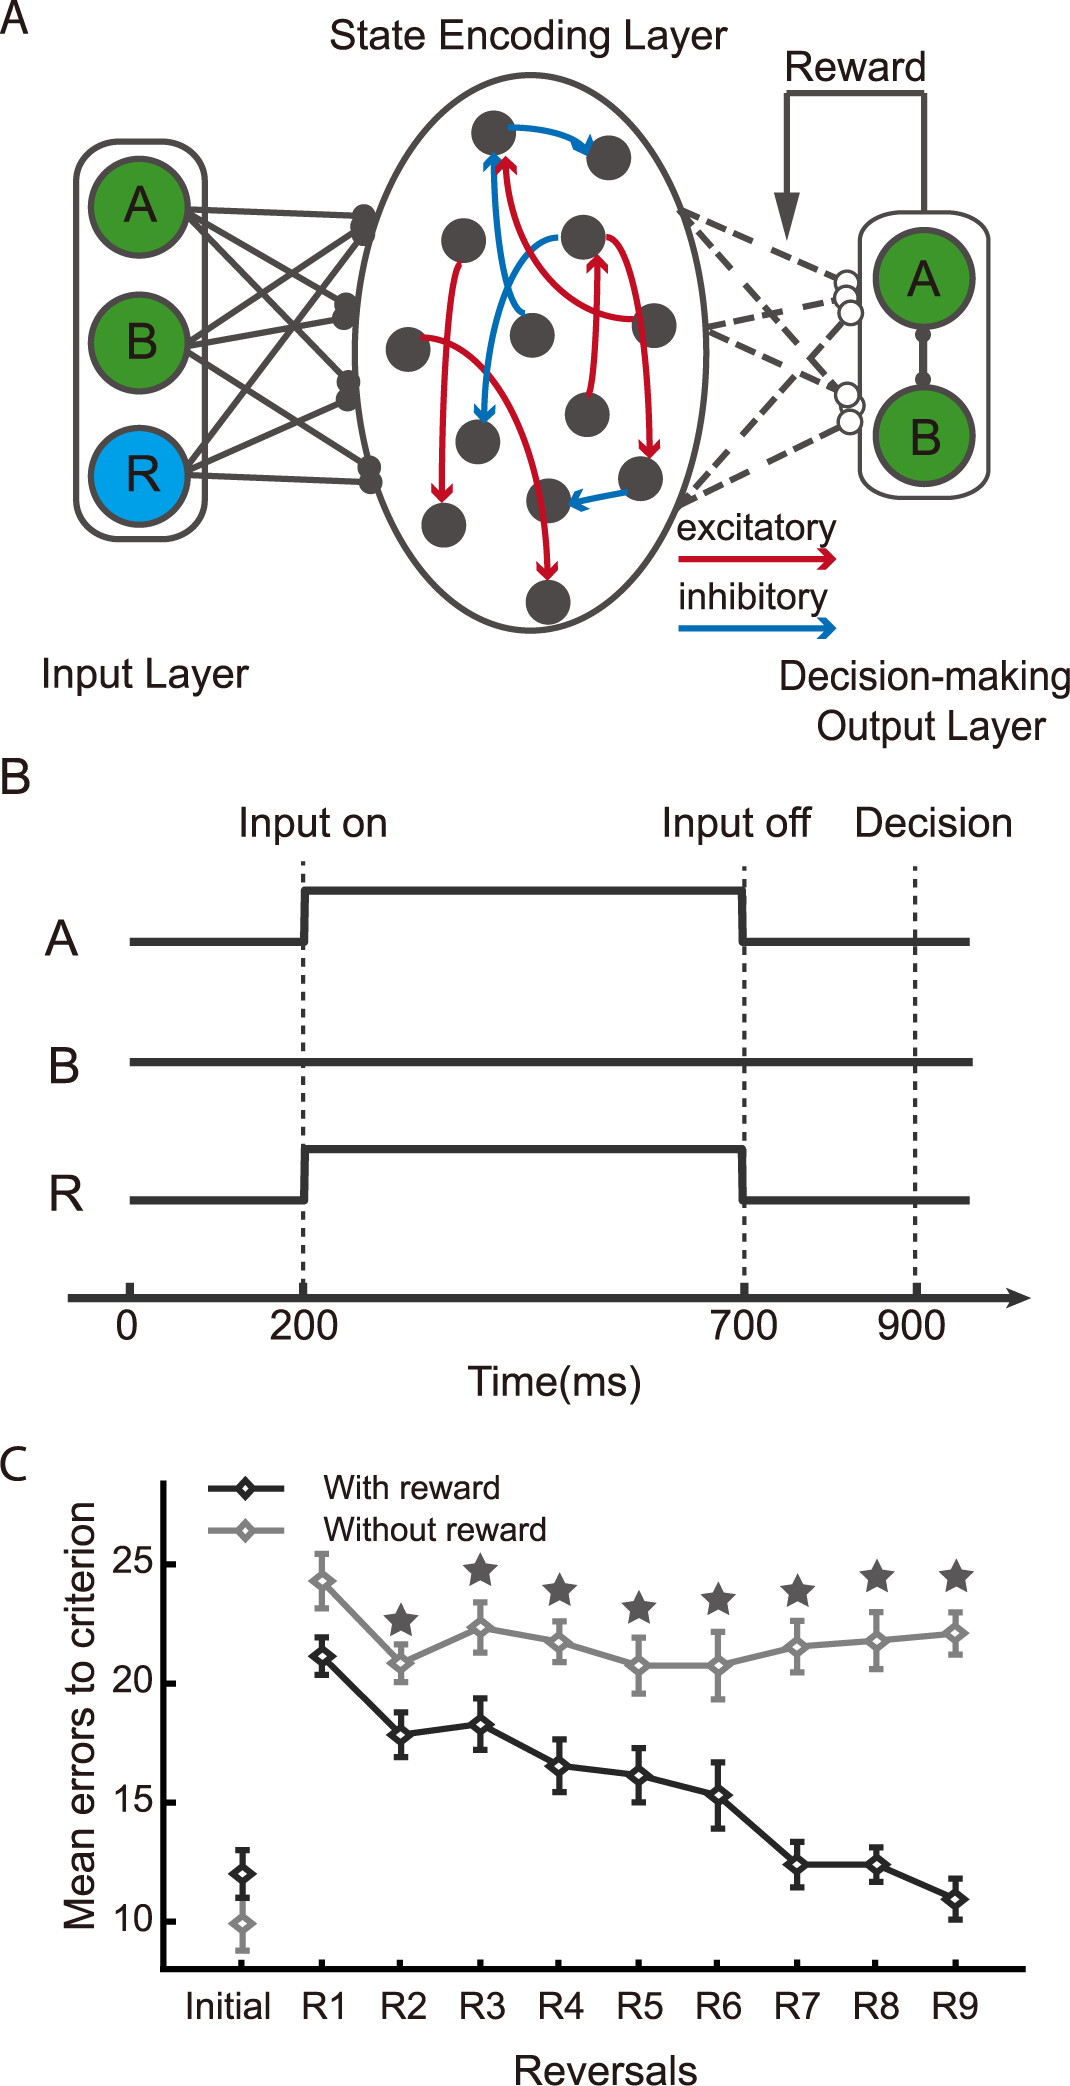
\includegraphics{journal_pcbi_1005925_g001.PNG}
\caption{A diagram of Zhang et. al's reservoir neural network architecture and experimental setup.}
\end{figure}

Their original MATLAB code is also available in the a public
\href{https://github.com/tyangLab/ReservoirNet_OFC_TaskState}{GitHub
repository}.

\hypertarget{mathematics}{%
\subsection{Mathematics}\label{mathematics}}

Below are the mathematical formulations used directly in the reservoir
neural network model. The network has N nodes whose activation value
\(x\) is represented by \begin{align}
\ \tau\frac{dx}{dt}= -x_i + g \sum_{j=1}^N w_{ij} y_j + w_i^{(i)}I + \sigma_{noise}dW_i \\
x(t + 1) = x(t) + \dot{x}(t)\Delta t
\end{align}

Where \(dW_i\) stands for white noise sampled from a uniform
distribution {[}0, 1{]} and \(\sigma_{noise}\) is its variance. \(y_i\)
is the firing rate of neuron \(i\), relative to a \(y_{min}=0\),
\(y_{max}=1\) and baseline firing rate \(y_0 = 0.1\). It is determined
by the following piecewise function: \begin{align}
y=   \left\{
\begin{array}{ll}
      y_0 + y_0 tanh(x/y_0) & x \leq 0   \\
      y_0 + (y_{max} - y_0)*tanh(\frac{x}{y_{max}- y_0}) & x > 0 \\
\end{array} 
\right.
\end{align}

The contributions of each node are then summed to \(v_k\). \(p_k\) then
is determined by performing a softmax on \(v_k\). \(p_k\) then becomes
the expected reward \(E[r_k]\) \begin{align}
v_k = \sum_{i=1}^N w_{out} * y_i \\
p_k = E[r_k] = \frac{e^{-\beta v_k}}{\sum_i e^{-\beta v_i}}
\end{align}

The final output elements \(z_k\) is either 1 with probability \(p_k\)
or 0 with probability \(1 - p_k\) The weighted random choice in this
experiment is between two actions \(a_k\): \(a_1=<0, 1>\) and
\(a_2=<1,0>\), where \(z_1 = 1\) means \(a_1\) was chose, and \(z_2=1\)
means \(a_2\) was chosen.

The weights on the output layer (\(w_{out}\)) are the only ones that are
plastic. These are only updated on the same timestep that the reward
\(r\) is administered because the mice do not receive any information
nor feedback when they refuse to lick, regardless of the texture
presented. The update is relative to the particular decision taken
\(z_k\) and whether a given neuron \(y_i\) had a firing rate greater
than the threshold \(y_{th}\). \begin{align}
\Delta w_{out} = \eta (r - E[r]) (y_i - y_{th}) z_k \\
w_{out}(n + 1) = w_{out}(n) + \Delta w_{out} \\
\end{align} Finally, the weights are normalized after each update:
\begin{align}
w_{out}(n) = \frac{w_{out}(n)}{\sqrt{\sum_{i=1}^N ||w_{out}(n)||^2}}
\end{align}

\hypertarget{implementation}{%
\subsection{Implementation}\label{implementation}}

Below I have directly implemented the formulated model as stated in the
paper and run a few trials using their parameter specifications.

    \begin{tcolorbox}[breakable, size=fbox, boxrule=1pt, pad at break*=1mm,colback=cellbackground, colframe=cellborder]
\prompt{In}{incolor}{1}{\hspace{4pt}}
\begin{Verbatim}[commandchars=\\\{\}]
\PY{c+c1}{\PYZsh{} Imports.}
\PY{o}{\PYZpc{}}\PY{k}{matplotlib} inline
\PY{k+kn}{import} \PY{n+nn}{numpy} \PY{k}{as} \PY{n+nn}{np}
\PY{k+kn}{import} \PY{n+nn}{pandas} \PY{k}{as} \PY{n+nn}{pd}
\PY{k+kn}{import} \PY{n+nn}{matplotlib}\PY{n+nn}{.}\PY{n+nn}{pyplot} \PY{k}{as} \PY{n+nn}{plt}
\PY{k+kn}{from} \PY{n+nn}{matplotlib} \PY{k}{import} \PY{n}{cm}
\PY{k+kn}{from} \PY{n+nn}{matplotlib}\PY{n+nn}{.}\PY{n+nn}{ticker} \PY{k}{import} \PY{n}{LinearLocator}\PY{p}{,} \PY{n}{FormatStrFormatter}
\PY{k+kn}{from} \PY{n+nn}{mpl\PYZus{}toolkits}\PY{n+nn}{.}\PY{n+nn}{mplot3d} \PY{k}{import} \PY{n}{Axes3D}
\PY{k+kn}{import} \PY{n+nn}{matplotlib}\PY{n+nn}{.}\PY{n+nn}{pyplot} \PY{k}{as} \PY{n+nn}{plt}
\PY{k+kn}{from} \PY{n+nn}{scipy}\PY{n+nn}{.}\PY{n+nn}{signal} \PY{k}{import} \PY{n}{butter}\PY{p}{,} \PY{n}{lfilter}\PY{p}{,} \PY{n}{freqz}
\PY{k+kn}{import} \PY{n+nn}{seaborn} \PY{k}{as} \PY{n+nn}{sns}
\PY{n}{sns}\PY{o}{.}\PY{n}{set}\PY{p}{(}\PY{p}{)}
\end{Verbatim}
\end{tcolorbox}

    \begin{tcolorbox}[breakable, size=fbox, boxrule=1pt, pad at break*=1mm,colback=cellbackground, colframe=cellborder]
\prompt{In}{incolor}{2}{\hspace{4pt}}
\begin{Verbatim}[commandchars=\\\{\}]
\PY{c+c1}{\PYZsh{} Experimental parameters.}

\PY{n}{num\PYZus{}trials} \PY{o}{=} \PY{l+m+mi}{1000} \PY{c+c1}{\PYZsh{} Original number: 1000}
\PY{n}{StopTrainingTrials} \PY{o}{=} \PY{l+m+mi}{5000}
\PY{n}{numReversed} \PY{o}{=} \PY{l+m+mi}{100}
\PY{n}{reinforcedSchedule} \PY{o}{=} \PY{l+m+mi}{1} \PY{c+c1}{\PYZsh{} determined or prob}
\PY{n}{withRF} \PY{o}{=} \PY{l+m+mi}{1}  \PY{c+c1}{\PYZsh{} reward feedback}
\PY{n}{numMod} \PY{o}{=} \PY{l+m+mi}{1}
\PY{n}{detail} \PY{o}{=} \PY{l+m+mi}{0}
\PY{n}{REinitial} \PY{o}{=} \PY{l+m+mi}{1}
\PY{n}{simutan}\PY{o}{=} \PY{l+m+mi}{1}
\PY{n}{blocking} \PY{o}{=} \PY{l+m+mi}{0} \PY{c+c1}{\PYZsh{} 0:no block, 1: random block,  2:A block,  3: AR block }

\PY{c+c1}{\PYZsh{} set the time}
\PY{n}{dt} \PY{o}{=} \PY{l+m+mf}{0.001}
\PY{n}{start} \PY{o}{=} \PY{l+m+mf}{0.2}    \PY{c+c1}{\PYZsh{} upon time of stimulus}
\PY{n}{sdur} \PY{o}{=} \PY{l+m+mf}{0.5}    \PY{c+c1}{\PYZsh{} duration of the stimulus}
\PY{n}{inter} \PY{o}{=} \PY{l+m+mi}{0}   \PY{c+c1}{\PYZsh{} interval between stimulus and reward}
\PY{n}{rdur} \PY{o}{=} \PY{l+m+mf}{0.5}    \PY{c+c1}{\PYZsh{} duration of reward input}
\PY{n}{delay} \PY{o}{=} \PY{l+m+mf}{0.2}   \PY{c+c1}{\PYZsh{} delay before decision}
\PY{n}{intertrial} \PY{o}{=} \PY{l+m+mi}{0}
\PY{n}{tau} \PY{o}{=} \PY{l+m+mf}{0.1} \PY{c+c1}{\PYZsh{} time constant }
\end{Verbatim}
\end{tcolorbox}

    \begin{tcolorbox}[breakable, size=fbox, boxrule=1pt, pad at break*=1mm,colback=cellbackground, colframe=cellborder]
\prompt{In}{incolor}{3}{\hspace{4pt}}
\begin{Verbatim}[commandchars=\\\{\}]
\PY{c+c1}{\PYZsh{} Model parameters from OFC paper for the reversal learning task}

\PY{n}{reservoir\PYZus{}network\PYZus{}params} \PY{o}{=} \PY{p}{\PYZob{}}
    \PY{l+s+s1}{\PYZsq{}}\PY{l+s+s1}{tau}\PY{l+s+s1}{\PYZsq{}}         \PY{p}{:} \PY{l+m+mf}{0.1}\PY{p}{,}         \PY{c+c1}{\PYZsh{} 100ms.}
    \PY{l+s+s1}{\PYZsq{}}\PY{l+s+s1}{dt}\PY{l+s+s1}{\PYZsq{}}          \PY{p}{:} \PY{l+m+mf}{0.001}\PY{p}{,}       \PY{c+c1}{\PYZsh{} 1ms.}
    \PY{l+s+s1}{\PYZsq{}}\PY{l+s+s1}{network gain}\PY{l+s+s1}{\PYZsq{}}\PY{p}{:} \PY{l+m+mi}{2}\PY{p}{,}           \PY{c+c1}{\PYZsh{} g}
    \PY{l+s+s1}{\PYZsq{}}\PY{l+s+s1}{training threshold}\PY{l+s+s1}{\PYZsq{}}\PY{p}{:} \PY{l+m+mf}{0.2}\PY{p}{,}   \PY{c+c1}{\PYZsh{} y\PYZus{}th}
    \PY{l+s+s1}{\PYZsq{}}\PY{l+s+s1}{temp parameter}\PY{l+s+s1}{\PYZsq{}}    \PY{p}{:} \PY{l+m+mi}{4}\PY{p}{,}     \PY{c+c1}{\PYZsh{} B (beta)}
    \PY{l+s+s1}{\PYZsq{}}\PY{l+s+s1}{learning rate}\PY{l+s+s1}{\PYZsq{}}     \PY{p}{:} \PY{l+m+mf}{0.001}\PY{p}{,} \PY{c+c1}{\PYZsh{} n (eta)}
    \PY{l+s+s1}{\PYZsq{}}\PY{l+s+s1}{max firing rate}\PY{l+s+s1}{\PYZsq{}}   \PY{p}{:} \PY{l+m+mi}{1}\PY{p}{,}     \PY{c+c1}{\PYZsh{} y\PYZus{}max}
    \PY{l+s+s1}{\PYZsq{}}\PY{l+s+s1}{base firing rate}\PY{l+s+s1}{\PYZsq{}}  \PY{p}{:} \PY{l+m+mf}{0.1}\PY{p}{,}   \PY{c+c1}{\PYZsh{} y\PYZus{}0}
    \PY{l+s+s1}{\PYZsq{}}\PY{l+s+s1}{noise gain}\PY{l+s+s1}{\PYZsq{}}  \PY{p}{:} \PY{l+m+mf}{0.01}\PY{p}{,}        \PY{c+c1}{\PYZsh{} sigma\PYZus{}noise}
    \PY{l+s+s1}{\PYZsq{}}\PY{l+s+s1}{initial noise gain}\PY{l+s+s1}{\PYZsq{}}\PY{p}{:} \PY{l+m+mf}{0.01}\PY{p}{,}  \PY{c+c1}{\PYZsh{} sigma\PYZus{}ini}
    \PY{l+s+s1}{\PYZsq{}}\PY{l+s+s1}{input gain}\PY{l+s+s1}{\PYZsq{}}  \PY{p}{:} \PY{l+m+mi}{4}\PY{p}{,}           \PY{c+c1}{\PYZsh{} g\PYZus{}IR        gain input \PYZhy{}\PYZgt{} reservoir}
    \PY{l+s+s1}{\PYZsq{}}\PY{l+s+s1}{input prob}\PY{l+s+s1}{\PYZsq{}}  \PY{p}{:} \PY{l+m+mf}{0.2}\PY{p}{,}         \PY{c+c1}{\PYZsh{} p\PYZus{}IR        prob input \PYZhy{}\PYZgt{} reservoir}
    \PY{l+s+s1}{\PYZsq{}}\PY{l+s+s1}{hidden layer prob}\PY{l+s+s1}{\PYZsq{}} \PY{p}{:} \PY{l+m+mf}{0.1}\PY{p}{,}   \PY{c+c1}{\PYZsh{} p           Probability of connection in hidden layer}
\PY{p}{\PYZcb{}}
\end{Verbatim}
\end{tcolorbox}

    \begin{tcolorbox}[breakable, size=fbox, boxrule=1pt, pad at break*=1mm,colback=cellbackground, colframe=cellborder]
\prompt{In}{incolor}{4}{\hspace{4pt}}
\begin{Verbatim}[commandchars=\\\{\}]
\PY{c+c1}{\PYZsh{} Helper functions.}

\PY{k}{def} \PY{n+nf}{sigmoid}\PY{p}{(}\PY{n}{x}\PY{p}{,} \PY{n}{x\PYZus{}0}\PY{o}{=}\PY{l+m+mi}{1}\PY{p}{)}\PY{p}{:}
    \PY{k}{return} \PY{l+m+mi}{1}\PY{o}{/}\PY{p}{(}\PY{l+m+mi}{1} \PY{o}{+} \PY{n}{np}\PY{o}{.}\PY{n}{exp}\PY{p}{(}\PY{n}{x}\PY{o}{/}\PY{n}{x\PYZus{}0}\PY{p}{)}\PY{p}{)}

\PY{k}{def} \PY{n+nf}{softmax}\PY{p}{(}\PY{n}{x}\PY{p}{,} \PY{n}{beta}\PY{p}{)}\PY{p}{:}
    \PY{n}{e} \PY{o}{=} \PY{n}{np}\PY{o}{.}\PY{n}{exp}\PY{p}{(}\PY{o}{\PYZhy{}}\PY{n}{beta} \PY{o}{*} \PY{n}{x}\PY{p}{)}
    \PY{k}{return} \PY{n}{e} \PY{o}{/} \PY{n}{e}\PY{o}{.}\PY{n}{sum}\PY{p}{(}\PY{p}{)}
  
\PY{k}{def} \PY{n+nf}{butter\PYZus{}lowpass}\PY{p}{(}\PY{n}{cutoff}\PY{p}{,} \PY{n}{fs}\PY{p}{,} \PY{n}{order}\PY{o}{=}\PY{l+m+mi}{5}\PY{p}{)}\PY{p}{:}
    \PY{n}{nyq} \PY{o}{=} \PY{l+m+mf}{0.5} \PY{o}{*} \PY{n}{fs}
    \PY{n}{normal\PYZus{}cutoff} \PY{o}{=} \PY{n}{cutoff} \PY{o}{/} \PY{n}{nyq}
    \PY{n}{b}\PY{p}{,} \PY{n}{a} \PY{o}{=} \PY{n}{butter}\PY{p}{(}\PY{n}{order}\PY{p}{,} \PY{n}{normal\PYZus{}cutoff}\PY{p}{,} \PY{n}{btype}\PY{o}{=}\PY{l+s+s1}{\PYZsq{}}\PY{l+s+s1}{low}\PY{l+s+s1}{\PYZsq{}}\PY{p}{,} \PY{n}{analog}\PY{o}{=}\PY{k+kc}{False}\PY{p}{)}
    \PY{k}{return} \PY{n}{b}\PY{p}{,} \PY{n}{a}

\PY{k}{def} \PY{n+nf}{butter\PYZus{}lowpass\PYZus{}filter}\PY{p}{(}\PY{n}{data}\PY{p}{,} \PY{n}{cutoff}\PY{p}{,} \PY{n}{fs}\PY{p}{,} \PY{n}{order}\PY{o}{=}\PY{l+m+mi}{5}\PY{p}{)}\PY{p}{:}
    \PY{n}{b}\PY{p}{,} \PY{n}{a} \PY{o}{=} \PY{n}{butter\PYZus{}lowpass}\PY{p}{(}\PY{n}{cutoff}\PY{p}{,} \PY{n}{fs}\PY{p}{,} \PY{n}{order}\PY{o}{=}\PY{n}{order}\PY{p}{)}
    \PY{n}{y} \PY{o}{=} \PY{n}{lfilter}\PY{p}{(}\PY{n}{b}\PY{p}{,} \PY{n}{a}\PY{p}{,} \PY{n}{data}\PY{p}{)}
    \PY{k}{return} \PY{n}{y}
  
\PY{k}{def} \PY{n+nf}{gaussian}\PY{p}{(}\PY{n}{mu}\PY{p}{,}\PY{n}{s2}\PY{p}{)}\PY{p}{:}
    \PY{k}{return} \PY{n}{np}\PY{o}{.}\PY{n}{exp}\PY{p}{(}\PY{o}{\PYZhy{}}\PY{n}{mu}\PY{o}{*}\PY{o}{*}\PY{l+m+mi}{2}\PY{o}{/}\PY{l+m+mi}{2}\PY{o}{/}\PY{n}{s2}\PY{p}{)} \PY{o}{/} \PY{n}{np}\PY{o}{.}\PY{n}{sqrt}\PY{p}{(}\PY{l+m+mi}{2} \PY{o}{*} \PY{n}{np}\PY{o}{.}\PY{n}{pi} \PY{o}{*} \PY{n}{s2}\PY{p}{)}

\PY{k}{def} \PY{n+nf}{smooth}\PY{p}{(}\PY{n}{x1}\PY{p}{,} \PY{n}{x2}\PY{p}{,} \PY{n}{y1}\PY{p}{,} \PY{n}{s2}\PY{p}{)}\PY{p}{:}
    \PY{n}{N2} \PY{o}{=} \PY{n+nb}{len}\PY{p}{(}\PY{n}{x2}\PY{p}{)}
    \PY{n}{y2} \PY{o}{=} \PY{n}{np}\PY{o}{.}\PY{n}{zeros}\PY{p}{(}\PY{n}{N2}\PY{p}{)}

    \PY{c+c1}{\PYZsh{} Check that the new data range does not exceed the old one}
    \PY{n}{rangeX1} \PY{o}{=} \PY{p}{[}\PY{n}{np}\PY{o}{.}\PY{n}{min}\PY{p}{(}\PY{n}{x1}\PY{p}{)}\PY{p}{,} \PY{n}{np}\PY{o}{.}\PY{n}{max}\PY{p}{(}\PY{n}{x1}\PY{p}{)}\PY{p}{]}
    \PY{n}{rangeX2} \PY{o}{=} \PY{p}{[}\PY{n}{np}\PY{o}{.}\PY{n}{min}\PY{p}{(}\PY{n}{x2}\PY{p}{)}\PY{p}{,} \PY{n}{np}\PY{o}{.}\PY{n}{max}\PY{p}{(}\PY{n}{x2}\PY{p}{)}\PY{p}{]}

    \PY{k}{for} \PY{n}{i2} \PY{o+ow}{in} \PY{n+nb}{range}\PY{p}{(}\PY{n}{x2}\PY{o}{.}\PY{n}{size}\PY{p}{)}\PY{p}{:}
        \PY{n}{w\PYZus{}ker} \PY{o}{=} \PY{n}{gaussian}\PY{p}{(}\PY{n}{x2}\PY{p}{[}\PY{n}{i2}\PY{p}{]} \PY{o}{\PYZhy{}} \PY{n}{x1}\PY{p}{,} \PY{n}{s2}\PY{p}{)}
        \PY{n}{w\PYZus{}ker} \PY{o}{/}\PY{o}{=} \PY{n}{np}\PY{o}{.}\PY{n}{sum}\PY{p}{(}\PY{n}{w\PYZus{}ker}\PY{p}{)}
        \PY{n}{y2}\PY{p}{[}\PY{n}{i2}\PY{p}{]} \PY{o}{=} \PY{n}{w\PYZus{}ker}\PY{o}{.}\PY{n}{dot}\PY{p}{(}\PY{n}{y1}\PY{p}{)}

    \PY{k}{return} \PY{n}{y2}
\end{Verbatim}
\end{tcolorbox}

    \begin{tcolorbox}[breakable, size=fbox, boxrule=1pt, pad at break*=1mm,colback=cellbackground, colframe=cellborder]
\prompt{In}{incolor}{5}{\hspace{4pt}}
\begin{Verbatim}[commandchars=\\\{\}]
\PY{c+c1}{\PYZsh{} Implementation of the OFC paper reservoir network.}

\PY{k}{class} \PY{n+nc}{OFCPaperNeuralNetwork}\PY{p}{(}\PY{n+nb}{object}\PY{p}{)}\PY{p}{:}
    \PY{k}{def} \PY{n+nf}{\PYZus{}\PYZus{}init\PYZus{}\PYZus{}}\PY{p}{(}\PY{n+nb+bp}{self}\PY{p}{,} \PY{n}{params}\PY{p}{,} \PY{n}{nodes}\PY{o}{=}\PY{l+m+mi}{500}\PY{p}{,} \PY{n}{input\PYZus{}dim}\PY{o}{=}\PY{l+m+mi}{2}\PY{p}{,} \PY{n}{output\PYZus{}dim}\PY{o}{=}\PY{l+m+mi}{2}\PY{p}{,} \PY{n}{reward\PYZus{}dim}\PY{o}{=}\PY{l+m+mi}{1}\PY{p}{)}\PY{p}{:}
        \PY{n+nb+bp}{self}\PY{o}{.}\PY{n}{output\PYZus{}dim} \PY{o}{=} \PY{n}{output\PYZus{}dim}
        \PY{n+nb+bp}{self}\PY{o}{.}\PY{n}{params} \PY{o}{=} \PY{n}{params}\PY{o}{.}\PY{n}{copy}\PY{p}{(}\PY{p}{)}
        \PY{n+nb+bp}{self}\PY{o}{.}\PY{n}{init\PYZus{}input\PYZus{}weights}\PY{p}{(}\PY{n}{input\PYZus{}dim} \PY{o}{+} \PY{n}{reward\PYZus{}dim}\PY{p}{,} \PY{n}{nodes}\PY{p}{)}
        \PY{n+nb+bp}{self}\PY{o}{.}\PY{n}{init\PYZus{}hidden\PYZus{}weights}\PY{p}{(}\PY{n}{nodes}\PY{p}{)}
        \PY{n+nb+bp}{self}\PY{o}{.}\PY{n}{init\PYZus{}neurons}\PY{p}{(}\PY{n}{nodes}\PY{p}{)}
        \PY{n+nb+bp}{self}\PY{o}{.}\PY{n}{init\PYZus{}output\PYZus{}weights}\PY{p}{(}\PY{n}{nodes}\PY{p}{,} \PY{n}{output\PYZus{}dim}\PY{p}{)}
        \PY{n+nb+bp}{self}\PY{o}{.}\PY{n}{exp\PYZus{}r} \PY{o}{=} \PY{n}{np}\PY{o}{.}\PY{n}{zeros}\PY{p}{(}\PY{n}{output\PYZus{}dim}\PY{p}{)}
        \PY{n+nb+bp}{self}\PY{o}{.}\PY{n}{z} \PY{o}{=} \PY{n}{np}\PY{o}{.}\PY{n}{zeros}\PY{p}{(}\PY{n}{output\PYZus{}dim}\PY{p}{)}

    \PY{k}{def} \PY{n+nf}{init\PYZus{}input\PYZus{}weights}\PY{p}{(}\PY{n+nb+bp}{self}\PY{p}{,} \PY{n}{input\PYZus{}dim}\PY{p}{,} \PY{n}{nodes}\PY{p}{)}\PY{p}{:}
        \PY{n}{std\PYZus{}dev} \PY{o}{=} \PY{n+nb+bp}{self}\PY{o}{.}\PY{n}{params}\PY{p}{[}\PY{l+s+s1}{\PYZsq{}}\PY{l+s+s1}{input gain}\PY{l+s+s1}{\PYZsq{}}\PY{p}{]}  \PY{c+c1}{\PYZsh{} The paper uses a variance of g\PYZus{}IR\PYZca{}2}
        \PY{n}{w\PYZus{}input} \PY{o}{=} \PY{n}{np}\PY{o}{.}\PY{n}{random}\PY{o}{.}\PY{n}{normal}\PY{p}{(}\PY{n}{loc}\PY{o}{=}\PY{l+m+mf}{0.0}\PY{p}{,} \PY{n}{scale}\PY{o}{=}\PY{n}{std\PYZus{}dev}\PY{p}{,} \PY{n}{size}\PY{o}{=}\PY{p}{(}\PY{n}{input\PYZus{}dim}\PY{p}{,} \PY{n}{nodes}\PY{p}{)}\PY{p}{)}
        \PY{n}{p\PYZus{}IR} \PY{o}{=} \PY{n+nb+bp}{self}\PY{o}{.}\PY{n}{params}\PY{p}{[}\PY{l+s+s1}{\PYZsq{}}\PY{l+s+s1}{input prob}\PY{l+s+s1}{\PYZsq{}}\PY{p}{]}
        \PY{n}{indices} \PY{o}{=} \PY{n}{np}\PY{o}{.}\PY{n}{random}\PY{o}{.}\PY{n}{choice}\PY{p}{(}\PY{p}{[}\PY{l+m+mi}{0}\PY{p}{,} \PY{l+m+mi}{1}\PY{p}{]}\PY{p}{,} \PY{n}{size}\PY{o}{=}\PY{n}{w\PYZus{}input}\PY{o}{.}\PY{n}{shape}\PY{p}{,} \PY{n}{p}\PY{o}{=}\PY{p}{[}\PY{l+m+mi}{1} \PY{o}{\PYZhy{}} \PY{n}{p\PYZus{}IR}\PY{p}{,} \PY{n}{p\PYZus{}IR}\PY{p}{]}\PY{p}{)} 
        \PY{n+nb+bp}{self}\PY{o}{.}\PY{n}{w\PYZus{}input} \PY{o}{=} \PY{n}{np}\PY{o}{.}\PY{n}{multiply}\PY{p}{(}\PY{n}{w\PYZus{}input}\PY{p}{,} \PY{n}{indices}\PY{p}{)}

    \PY{k}{def} \PY{n+nf}{init\PYZus{}hidden\PYZus{}weights}\PY{p}{(}\PY{n+nb+bp}{self}\PY{p}{,} \PY{n}{nodes}\PY{p}{)}\PY{p}{:}
        \PY{n}{g} \PY{o}{=} \PY{n+nb+bp}{self}\PY{o}{.}\PY{n}{params}\PY{p}{[}\PY{l+s+s1}{\PYZsq{}}\PY{l+s+s1}{initial noise gain}\PY{l+s+s1}{\PYZsq{}}\PY{p}{]}
        \PY{n}{p} \PY{o}{=} \PY{n+nb+bp}{self}\PY{o}{.}\PY{n}{params}\PY{p}{[}\PY{l+s+s1}{\PYZsq{}}\PY{l+s+s1}{hidden layer prob}\PY{l+s+s1}{\PYZsq{}}\PY{p}{]}
        \PY{n}{std\PYZus{}dev} \PY{o}{=} \PY{n}{g} \PY{o}{/} \PY{n}{np}\PY{o}{.}\PY{n}{sqrt}\PY{p}{(}\PY{n}{p} \PY{o}{*} \PY{n}{nodes}\PY{p}{)} \PY{c+c1}{\PYZsh{} The paper uses a variance of g\PYZca{}2/(p*N)}
        \PY{n}{W} \PY{o}{=} \PY{n}{np}\PY{o}{.}\PY{n}{random}\PY{o}{.}\PY{n}{normal}\PY{p}{(}\PY{n}{loc}\PY{o}{=}\PY{l+m+mf}{0.0}\PY{p}{,} \PY{n}{scale}\PY{o}{=}\PY{n}{std\PYZus{}dev}\PY{p}{,} \PY{n}{size}\PY{o}{=}\PY{p}{(}\PY{n}{nodes}\PY{p}{,} \PY{n}{nodes}\PY{p}{)}\PY{p}{)}
        \PY{n}{indices} \PY{o}{=} \PY{n}{np}\PY{o}{.}\PY{n}{random}\PY{o}{.}\PY{n}{choice}\PY{p}{(}\PY{p}{[}\PY{l+m+mi}{0}\PY{p}{,} \PY{l+m+mi}{1}\PY{p}{]}\PY{p}{,} \PY{n}{size}\PY{o}{=}\PY{n}{W}\PY{o}{.}\PY{n}{shape}\PY{p}{,} \PY{n}{p}\PY{o}{=}\PY{p}{[}\PY{l+m+mi}{1} \PY{o}{\PYZhy{}} \PY{n}{p}\PY{p}{,} \PY{n}{p}\PY{p}{]}\PY{p}{)} 
        \PY{n+nb+bp}{self}\PY{o}{.}\PY{n}{hidden\PYZus{}weights} \PY{o}{=} \PY{n}{np}\PY{o}{.}\PY{n}{multiply}\PY{p}{(}\PY{n}{W}\PY{p}{,} \PY{n}{indices}\PY{p}{)}

    \PY{k}{def} \PY{n+nf}{init\PYZus{}neurons}\PY{p}{(}\PY{n+nb+bp}{self}\PY{p}{,} \PY{n}{nodes}\PY{p}{)}\PY{p}{:}
        \PY{n}{std\PYZus{}dev} \PY{o}{=} \PY{n+nb+bp}{self}\PY{o}{.}\PY{n}{params}\PY{p}{[}\PY{l+s+s1}{\PYZsq{}}\PY{l+s+s1}{initial noise gain}\PY{l+s+s1}{\PYZsq{}}\PY{p}{]} \PY{c+c1}{\PYZsh{} The paper uses a variance of sigma\PYZus{}ini\PYZca{}2}
        \PY{n}{x} \PY{o}{=} \PY{n}{np}\PY{o}{.}\PY{n}{random}\PY{o}{.}\PY{n}{normal}\PY{p}{(}\PY{n}{loc}\PY{o}{=}\PY{l+m+mf}{0.0}\PY{p}{,} \PY{n}{scale}\PY{o}{=}\PY{n}{std\PYZus{}dev}\PY{p}{,} \PY{n}{size}\PY{o}{=}\PY{n}{nodes}\PY{p}{)}
        \PY{n}{y} \PY{o}{=} \PY{n}{np}\PY{o}{.}\PY{n}{ones}\PY{p}{(}\PY{n}{nodes}\PY{p}{)} \PY{o}{*} \PY{n+nb+bp}{self}\PY{o}{.}\PY{n}{params}\PY{p}{[}\PY{l+s+s1}{\PYZsq{}}\PY{l+s+s1}{base firing rate}\PY{l+s+s1}{\PYZsq{}}\PY{p}{]}
        \PY{n+nb+bp}{self}\PY{o}{.}\PY{n}{x} \PY{o}{=} \PY{n}{x}
        \PY{n+nb+bp}{self}\PY{o}{.}\PY{n}{y} \PY{o}{=} \PY{n}{y}

    \PY{k}{def} \PY{n+nf}{init\PYZus{}output\PYZus{}weights}\PY{p}{(}\PY{n+nb+bp}{self}\PY{p}{,} \PY{n}{nodes}\PY{p}{,} \PY{n}{output\PYZus{}dim}\PY{p}{)}\PY{p}{:}
        \PY{n}{W} \PY{o}{=} \PY{n}{np}\PY{o}{.}\PY{n}{random}\PY{o}{.}\PY{n}{normal}\PY{p}{(}\PY{n}{loc}\PY{o}{=}\PY{l+m+mf}{0.0}\PY{p}{,} \PY{n}{scale}\PY{o}{=}\PY{l+m+mi}{1}\PY{p}{,} \PY{n}{size}\PY{o}{=}\PY{p}{(}\PY{n}{nodes}\PY{p}{,} \PY{n}{output\PYZus{}dim}\PY{p}{)}\PY{p}{)}
        \PY{c+c1}{\PYZsh{} According to the paper: normalize according to the squared sum of the weights for each output node.}
        \PY{n}{W} \PY{o}{=} \PY{n}{W}\PY{o}{/}\PY{n}{np}\PY{o}{.}\PY{n}{sqrt}\PY{p}{(}\PY{n}{np}\PY{o}{.}\PY{n}{square}\PY{p}{(}\PY{n}{W}\PY{p}{)}\PY{o}{.}\PY{n}{sum}\PY{p}{(}\PY{n}{axis}\PY{o}{=}\PY{l+m+mi}{0}\PY{p}{)}\PY{p}{)}
        \PY{n+nb+bp}{self}\PY{o}{.}\PY{n}{output\PYZus{}weights} \PY{o}{=} \PY{n}{W}
    
    \PY{k}{def} \PY{n+nf}{step}\PY{p}{(}\PY{n+nb+bp}{self}\PY{p}{,} \PY{n}{I}\PY{o}{=}\PY{l+m+mi}{0}\PY{p}{)}\PY{p}{:}
        \PY{k}{if} \PY{n}{np}\PY{o}{.}\PY{n}{array\PYZus{}equal}\PY{p}{(}\PY{n}{I}\PY{p}{,} \PY{l+m+mi}{0}\PY{p}{)}\PY{p}{:}
            \PY{n}{I} \PY{o}{=} \PY{n}{np}\PY{o}{.}\PY{n}{zeros}\PY{p}{(}\PY{n+nb+bp}{self}\PY{o}{.}\PY{n}{w\PYZus{}input}\PY{o}{.}\PY{n}{shape}\PY{p}{[}\PY{l+m+mi}{0}\PY{p}{]}\PY{p}{)}

        \PY{n}{tau} \PY{o}{=} \PY{n+nb+bp}{self}\PY{o}{.}\PY{n}{params}\PY{p}{[}\PY{l+s+s1}{\PYZsq{}}\PY{l+s+s1}{tau}\PY{l+s+s1}{\PYZsq{}}\PY{p}{]}
        \PY{n}{dt} \PY{o}{=} \PY{n+nb+bp}{self}\PY{o}{.}\PY{n}{params}\PY{p}{[}\PY{l+s+s1}{\PYZsq{}}\PY{l+s+s1}{dt}\PY{l+s+s1}{\PYZsq{}}\PY{p}{]}
        \PY{n}{g} \PY{o}{=} \PY{n+nb+bp}{self}\PY{o}{.}\PY{n}{params}\PY{p}{[}\PY{l+s+s1}{\PYZsq{}}\PY{l+s+s1}{network gain}\PY{l+s+s1}{\PYZsq{}}\PY{p}{]}
        \PY{n}{sigma\PYZus{}noise} \PY{o}{=} \PY{n+nb+bp}{self}\PY{o}{.}\PY{n}{params}\PY{p}{[}\PY{l+s+s1}{\PYZsq{}}\PY{l+s+s1}{noise gain}\PY{l+s+s1}{\PYZsq{}}\PY{p}{]}
        \PY{n}{y\PYZus{}0} \PY{o}{=} \PY{n+nb+bp}{self}\PY{o}{.}\PY{n}{params}\PY{p}{[}\PY{l+s+s1}{\PYZsq{}}\PY{l+s+s1}{base firing rate}\PY{l+s+s1}{\PYZsq{}}\PY{p}{]}
        \PY{n}{y\PYZus{}max} \PY{o}{=} \PY{n+nb+bp}{self}\PY{o}{.}\PY{n}{params}\PY{p}{[}\PY{l+s+s1}{\PYZsq{}}\PY{l+s+s1}{max firing rate}\PY{l+s+s1}{\PYZsq{}}\PY{p}{]}
        
        \PY{n}{white\PYZus{}noise} \PY{o}{=} \PY{n}{np}\PY{o}{.}\PY{n}{random}\PY{o}{.}\PY{n}{randint}\PY{p}{(}\PY{l+m+mi}{0}\PY{p}{,} \PY{n}{high}\PY{o}{=}\PY{p}{(}\PY{l+m+mi}{1} \PY{o}{+} \PY{l+m+mi}{1}\PY{p}{)}\PY{p}{,} \PY{n}{size}\PY{o}{=}\PY{n+nb+bp}{self}\PY{o}{.}\PY{n}{x}\PY{o}{.}\PY{n}{size}\PY{p}{)}
        
        \PY{n}{dx\PYZus{}dt} \PY{o}{=} \PY{l+m+mi}{1}\PY{o}{/}\PY{n}{tau} \PY{o}{*} \PY{p}{(}\PY{o}{\PYZhy{}}\PY{n+nb+bp}{self}\PY{o}{.}\PY{n}{x} \PY{o}{+} \PY{n}{g} \PY{o}{*} \PY{n}{np}\PY{o}{.}\PY{n}{dot}\PY{p}{(}\PY{n+nb+bp}{self}\PY{o}{.}\PY{n}{hidden\PYZus{}weights}\PY{p}{,} \PY{n+nb+bp}{self}\PY{o}{.}\PY{n}{y}\PY{p}{)} 
                         \PY{o}{+} \PY{n}{np}\PY{o}{.}\PY{n}{dot}\PY{p}{(}\PY{n+nb+bp}{self}\PY{o}{.}\PY{n}{w\PYZus{}input}\PY{o}{.}\PY{n}{T}\PY{p}{,} \PY{n}{I}\PY{p}{)} 
                         \PY{o}{+} \PY{n}{sigma\PYZus{}noise} \PY{o}{*} \PY{n}{white\PYZus{}noise}\PY{p}{)}
        \PY{n+nb+bp}{self}\PY{o}{.}\PY{n}{x} \PY{o}{+}\PY{o}{=} \PY{n}{dx\PYZus{}dt} \PY{o}{*} \PY{n}{dt}
        
        \PY{n}{y\PYZus{}conditions} \PY{o}{=}\PY{p}{[}\PY{n+nb+bp}{self}\PY{o}{.}\PY{n}{x} \PY{o}{\PYZlt{}}\PY{o}{=} \PY{l+m+mi}{0}\PY{p}{,} \PY{n+nb+bp}{self}\PY{o}{.}\PY{n}{x} \PY{o}{\PYZgt{}} \PY{l+m+mi}{0}\PY{p}{]}
        \PY{n}{y\PYZus{}functions} \PY{o}{=}\PY{p}{[}
            \PY{k}{lambda} \PY{n}{x}\PY{p}{:} \PY{n}{y\PYZus{}0} \PY{o}{+} \PY{n}{y\PYZus{}0} \PY{o}{*} \PY{n}{np}\PY{o}{.}\PY{n}{tanh}\PY{p}{(}\PY{n}{x}\PY{o}{/}\PY{n}{y\PYZus{}0}\PY{p}{)}\PY{p}{,}
            \PY{k}{lambda} \PY{n}{x}\PY{p}{:} \PY{n}{y\PYZus{}0} \PY{o}{+} \PY{p}{(}\PY{n}{y\PYZus{}max} \PY{o}{\PYZhy{}} \PY{n}{y\PYZus{}0}\PY{p}{)} \PY{o}{*} \PY{n}{np}\PY{o}{.}\PY{n}{tanh}\PY{p}{(}\PY{n}{x}\PY{o}{/}\PY{p}{(}\PY{n}{y\PYZus{}max} \PY{o}{\PYZhy{}} \PY{n}{y\PYZus{}0}\PY{p}{)}\PY{p}{)}
        \PY{p}{]}
        \PY{n+nb+bp}{self}\PY{o}{.}\PY{n}{y} \PY{o}{=} \PY{n}{np}\PY{o}{.}\PY{n}{piecewise}\PY{p}{(}\PY{n+nb+bp}{self}\PY{o}{.}\PY{n}{x}\PY{p}{,} \PY{n}{y\PYZus{}conditions}\PY{p}{,} \PY{n}{y\PYZus{}functions}\PY{p}{)}
        
        \PY{n}{v\PYZus{}k} \PY{o}{=} \PY{n}{np}\PY{o}{.}\PY{n}{dot}\PY{p}{(}\PY{n+nb+bp}{self}\PY{o}{.}\PY{n}{y}\PY{p}{,} \PY{n+nb+bp}{self}\PY{o}{.}\PY{n}{output\PYZus{}weights}\PY{p}{)}
        \PY{n}{beta} \PY{o}{=} \PY{n+nb+bp}{self}\PY{o}{.}\PY{n}{params}\PY{p}{[}\PY{l+s+s1}{\PYZsq{}}\PY{l+s+s1}{temp parameter}\PY{l+s+s1}{\PYZsq{}}\PY{p}{]}
        \PY{n}{p\PYZus{}k} \PY{o}{=} \PY{n}{softmax}\PY{p}{(}\PY{n}{v\PYZus{}k}\PY{p}{,} \PY{n}{beta}\PY{p}{)}
        
        \PY{c+c1}{\PYZsh{}self.z = np.greater\PYZus{}equal(p\PYZus{}k, p\PYZus{}k.max()).astype(float)}
        \PY{n}{choice\PYZus{}idx} \PY{o}{=} \PY{n}{np}\PY{o}{.}\PY{n}{random}\PY{o}{.}\PY{n}{choice}\PY{p}{(}\PY{n}{p\PYZus{}k}\PY{o}{.}\PY{n}{shape}\PY{p}{[}\PY{l+m+mi}{0}\PY{p}{]}\PY{p}{,} \PY{n}{p}\PY{o}{=}\PY{n}{p\PYZus{}k}\PY{p}{)}
        \PY{n+nb+bp}{self}\PY{o}{.}\PY{n}{z} \PY{o}{=} \PY{n}{np}\PY{o}{.}\PY{n}{zeros}\PY{p}{(}\PY{n}{p\PYZus{}k}\PY{o}{.}\PY{n}{shape}\PY{p}{)}
        \PY{n+nb+bp}{self}\PY{o}{.}\PY{n}{z}\PY{p}{[}\PY{n}{choice\PYZus{}idx}\PY{p}{]} \PY{o}{=} \PY{l+m+mi}{1}
         
            
        \PY{n+nb+bp}{self}\PY{o}{.}\PY{n}{exp\PYZus{}r} \PY{o}{=} \PY{n}{p\PYZus{}k}
        \PY{k}{return} \PY{n+nb+bp}{self}\PY{o}{.}\PY{n}{z}

    \PY{k}{def} \PY{n+nf}{receive\PYZus{}reward}\PY{p}{(}\PY{n+nb+bp}{self}\PY{p}{,} \PY{n}{r}\PY{p}{)}\PY{p}{:}
        \PY{n+nb+bp}{self}\PY{o}{.}\PY{n}{update\PYZus{}weights}\PY{p}{(}\PY{n}{r}\PY{p}{)}

    \PY{k}{def} \PY{n+nf}{update\PYZus{}weights}\PY{p}{(}\PY{n+nb+bp}{self}\PY{p}{,} \PY{n}{r}\PY{p}{)}\PY{p}{:}
        \PY{n}{row\PYZus{}vec} \PY{o}{=} \PY{n+nb+bp}{self}\PY{o}{.}\PY{n}{y} \PY{o}{\PYZhy{}} \PY{n+nb+bp}{self}\PY{o}{.}\PY{n}{params}\PY{p}{[}\PY{l+s+s1}{\PYZsq{}}\PY{l+s+s1}{training threshold}\PY{l+s+s1}{\PYZsq{}}\PY{p}{]}
        \PY{n}{col\PYZus{}vec} \PY{o}{=} \PY{n}{np}\PY{o}{.}\PY{n}{multiply}\PY{p}{(}\PY{p}{(}\PY{n}{r} \PY{o}{\PYZhy{}} \PY{n+nb+bp}{self}\PY{o}{.}\PY{n}{exp\PYZus{}r}\PY{p}{)}\PY{p}{,} \PY{n+nb+bp}{self}\PY{o}{.}\PY{n}{z}\PY{p}{)}
        \PY{n}{delta\PYZus{}w} \PY{o}{=} \PY{n+nb+bp}{self}\PY{o}{.}\PY{n}{params}\PY{p}{[}\PY{l+s+s1}{\PYZsq{}}\PY{l+s+s1}{learning rate}\PY{l+s+s1}{\PYZsq{}}\PY{p}{]} \PY{o}{*} \PY{n}{np}\PY{o}{.}\PY{n}{outer}\PY{p}{(}\PY{n}{row\PYZus{}vec}\PY{p}{,} \PY{n}{col\PYZus{}vec}\PY{p}{)}
        \PY{n+nb+bp}{self}\PY{o}{.}\PY{n}{output\PYZus{}weights} \PY{o}{+}\PY{o}{=} \PY{n}{delta\PYZus{}w}
          
\PY{c+c1}{\PYZsh{}         delta\PYZus{}w = self.params[\PYZsq{}learning rate\PYZsq{}] * np.outer((r \PYZhy{} self.exp\PYZus{}r),}
\PY{c+c1}{\PYZsh{}           (self.y \PYZhy{} self.params[\PYZsq{}training threshold\PYZsq{}]))}
\PY{c+c1}{\PYZsh{}         delta\PYZus{}w = np.multiply(delta\PYZus{}w.T, self.z)}
\PY{c+c1}{\PYZsh{}         self.output\PYZus{}weights += delta\PYZus{}w}

        \PY{c+c1}{\PYZsh{} Normalize weights}
        \PY{n+nb+bp}{self}\PY{o}{.}\PY{n}{output\PYZus{}weights} \PY{o}{/}\PY{o}{=} \PY{n}{np}\PY{o}{.}\PY{n}{linalg}\PY{o}{.}\PY{n}{norm}\PY{p}{(}\PY{n+nb+bp}{self}\PY{o}{.}\PY{n}{output\PYZus{}weights}\PY{p}{)}

    \PY{k}{def} \PY{n+nf}{get\PYZus{}output}\PY{p}{(}\PY{n+nb+bp}{self}\PY{p}{,} \PY{n}{exp}\PY{o}{=}\PY{k+kc}{False}\PY{p}{)}\PY{p}{:}
        \PY{k}{if} \PY{n}{exp}\PY{p}{:}
            \PY{k}{return} \PY{n+nb+bp}{self}\PY{o}{.}\PY{n}{z}\PY{p}{,} \PY{n+nb+bp}{self}\PY{o}{.}\PY{n}{exp\PYZus{}r}
        \PY{k}{else}\PY{p}{:}
            \PY{k}{return} \PY{n+nb+bp}{self}\PY{o}{.}\PY{n}{z}
\end{Verbatim}
\end{tcolorbox}

    \begin{tcolorbox}[breakable, size=fbox, boxrule=1pt, pad at break*=1mm,colback=cellbackground, colframe=cellborder]
\prompt{In}{incolor}{6}{\hspace{4pt}}
\begin{Verbatim}[commandchars=\\\{\}]
\PY{c+c1}{\PYZsh{} Experiment function.}

\PY{k}{def} \PY{n+nf}{simple\PYZus{}experiment}\PY{p}{(}\PY{n}{I}\PY{p}{,} \PY{n}{T}\PY{o}{=}\PY{l+m+mi}{1000}\PY{p}{,} \PY{n}{num\PYZus{}trials}\PY{o}{=}\PY{l+m+mi}{3000}\PY{p}{,} \PY{n}{net}\PY{o}{=}\PY{k+kc}{None}\PY{p}{,} \PY{n}{contingency}\PY{o}{=}\PY{k+kc}{None}\PY{p}{,} 
                      \PY{n}{input\PYZus{}reward}\PY{o}{=}\PY{k+kc}{True}\PY{p}{)}\PY{p}{:}
    \PY{n}{r\PYZus{}hist} \PY{o}{=} \PY{p}{[}\PY{p}{]}
    \PY{n}{decision\PYZus{}hist} \PY{o}{=} \PY{p}{[}\PY{p}{]}
    \PY{n}{exp\PYZus{}hist} \PY{o}{=} \PY{p}{[}\PY{p}{]}
    \PY{n}{r} \PY{o}{=} \PY{l+m+mi}{0}

    \PY{k}{for} \PY{n}{trial} \PY{o+ow}{in} \PY{n+nb}{range}\PY{p}{(}\PY{n}{num\PYZus{}trials}\PY{p}{)}\PY{p}{:}
        \PY{n}{index} \PY{o}{=} \PY{n}{np}\PY{o}{.}\PY{n}{random}\PY{o}{.}\PY{n}{randint}\PY{p}{(}\PY{n}{I}\PY{o}{.}\PY{n}{shape}\PY{p}{[}\PY{l+m+mi}{0}\PY{p}{]}\PY{p}{)}
        \PY{n}{text\PYZus{}input} \PY{o}{=} \PY{n}{I}\PY{p}{[}\PY{n}{index}\PY{p}{]}
        \PY{n}{exp\PYZus{}output} \PY{o}{=} \PY{n}{contingency}\PY{p}{[}\PY{n}{index}\PY{p}{]}
        
        \PY{n}{decision} \PY{o}{=} \PY{l+m+mi}{0}
        \PY{n}{expectation} \PY{o}{=} \PY{l+m+mi}{0}

        \PY{k}{for} \PY{n}{ms} \PY{o+ow}{in} \PY{n+nb}{range}\PY{p}{(}\PY{n}{T}\PY{p}{)}\PY{p}{:}
            \PY{c+c1}{\PYZsh{} Initial rest period (0 \PYZhy{} 200ms) of trial}
            \PY{k}{if} \PY{n}{ms} \PY{o}{\PYZlt{}} \PY{p}{(}\PY{n}{T} \PY{o}{*} \PY{n}{delay}\PY{p}{)}\PY{p}{:}
                \PY{n}{net}\PY{o}{.}\PY{n}{step}\PY{p}{(}\PY{p}{)}
                \PY{k}{continue}

            \PY{c+c1}{\PYZsh{} Apply input for the trial (200ms \PYZhy{} 700ms)}
            \PY{k}{if} \PY{l+m+mi}{200} \PY{o}{\PYZlt{}}\PY{o}{=} \PY{n}{ms} \PY{o}{\PYZlt{}}\PY{o}{=} \PY{l+m+mi}{700}\PY{p}{:}
                \PY{k}{if} \PY{n}{input\PYZus{}reward}\PY{p}{:}
                  \PY{n}{net}\PY{o}{.}\PY{n}{step}\PY{p}{(}\PY{n}{np}\PY{o}{.}\PY{n}{append}\PY{p}{(}\PY{n}{text\PYZus{}input}\PY{p}{,} \PY{n}{r}\PY{p}{)}\PY{p}{)}
                \PY{k}{else}\PY{p}{:}
                  \PY{n}{net}\PY{o}{.}\PY{n}{step}\PY{p}{(}\PY{n}{text\PYZus{}input}\PY{p}{)}
                \PY{k}{continue}

            \PY{c+c1}{\PYZsh{} Measure output of the network (900ms)}
            \PY{k}{if} \PY{n}{ms} \PY{o}{==} \PY{l+m+mi}{900}\PY{p}{:}
                \PY{n}{net}\PY{o}{.}\PY{n}{step}\PY{p}{(}\PY{p}{)}
                \PY{n}{decision}\PY{p}{,} \PY{n}{expectation} \PY{o}{=} \PY{n}{net}\PY{o}{.}\PY{n}{get\PYZus{}output}\PY{p}{(}\PY{n}{exp}\PY{o}{=}\PY{k+kc}{True}\PY{p}{)}
                \PY{n}{r} \PY{o}{=} \PY{n+nb}{int}\PY{p}{(}\PY{n}{np}\PY{o}{.}\PY{n}{array\PYZus{}equal}\PY{p}{(}\PY{n}{decision}\PY{p}{,} \PY{n}{exp\PYZus{}output}\PY{p}{)}\PY{p}{)}
                \PY{n}{net}\PY{o}{.}\PY{n}{receive\PYZus{}reward}\PY{p}{(}\PY{n}{r}\PY{p}{)}
                \PY{c+c1}{\PYZsh{}decision\PYZus{}hist += [decision]}
                \PY{c+c1}{\PYZsh{}exp\PYZus{}hist += [expectation]}
                \PY{k}{continue}

            \PY{k}{if} \PY{n}{ms} \PY{o}{\PYZgt{}} \PY{l+m+mi}{900}\PY{p}{:}
\PY{c+c1}{\PYZsh{}               net.receive\PYZus{}reward(r)}
                \PY{n}{net}\PY{o}{.}\PY{n}{step}\PY{p}{(}\PY{p}{)}
                \PY{k}{continue}
            
            \PY{c+c1}{\PYZsh{} If nothing needs to happen, move forward a timestep.}
            \PY{n}{net}\PY{o}{.}\PY{n}{step}\PY{p}{(}\PY{p}{)}
      
        \PY{n}{r\PYZus{}hist} \PY{o}{+}\PY{o}{=} \PY{p}{[}\PY{n}{r}\PY{p}{]}
        \PY{n}{decision\PYZus{}hist} \PY{o}{+}\PY{o}{=} \PY{p}{[}\PY{n}{decision}\PY{p}{]}
        \PY{n}{exp\PYZus{}hist} \PY{o}{+}\PY{o}{=} \PY{p}{[}\PY{n}{expectation}\PY{p}{]}
    
    \PY{n}{r\PYZus{}hist} \PY{o}{=} \PY{n}{np}\PY{o}{.}\PY{n}{array}\PY{p}{(}\PY{n}{r\PYZus{}hist}\PY{p}{)}
    \PY{n}{decision\PYZus{}hist} \PY{o}{=} \PY{n}{np}\PY{o}{.}\PY{n}{array}\PY{p}{(}\PY{n}{decision\PYZus{}hist}\PY{p}{)}
    \PY{n}{exp\PYZus{}hist} \PY{o}{=} \PY{n}{np}\PY{o}{.}\PY{n}{array}\PY{p}{(}\PY{n}{exp\PYZus{}hist}\PY{p}{)}
    \PY{k}{return} \PY{n}{r\PYZus{}hist}\PY{p}{,} \PY{n}{decision\PYZus{}hist}\PY{p}{,} \PY{n}{exp\PYZus{}hist}
\end{Verbatim}
\end{tcolorbox}

    \begin{tcolorbox}[breakable, size=fbox, boxrule=1pt, pad at break*=1mm,colback=cellbackground, colframe=cellborder]
\prompt{In}{incolor}{7}{\hspace{4pt}}
\begin{Verbatim}[commandchars=\\\{\}]
\PY{c+c1}{\PYZsh{} Inputs.}
\PY{n}{I\PYZus{}1} \PY{o}{=} \PY{n}{np}\PY{o}{.}\PY{n}{array}\PY{p}{(}\PY{p}{[}\PY{l+m+mi}{1}\PY{p}{,} \PY{l+m+mi}{0}\PY{p}{]}\PY{p}{)}
\PY{n}{I\PYZus{}2} \PY{o}{=} \PY{n}{np}\PY{o}{.}\PY{n}{array}\PY{p}{(}\PY{p}{[}\PY{l+m+mi}{0}\PY{p}{,} \PY{l+m+mi}{1}\PY{p}{]}\PY{p}{)}

\PY{n}{I} \PY{o}{=} \PY{n}{np}\PY{o}{.}\PY{n}{array}\PY{p}{(}\PY{p}{[}\PY{n}{I\PYZus{}1}\PY{p}{,} \PY{n}{I\PYZus{}2}\PY{p}{]}\PY{p}{)}


\PY{c+c1}{\PYZsh{} Outpus.}
\PY{n}{A\PYZus{}1} \PY{o}{=} \PY{n}{np}\PY{o}{.}\PY{n}{array}\PY{p}{(}\PY{p}{[}\PY{l+m+mi}{1}\PY{p}{,} \PY{l+m+mi}{0}\PY{p}{]}\PY{p}{)}
\PY{n}{A\PYZus{}2} \PY{o}{=} \PY{n}{np}\PY{o}{.}\PY{n}{array}\PY{p}{(}\PY{p}{[}\PY{l+m+mi}{0}\PY{p}{,} \PY{l+m+mi}{1}\PY{p}{]}\PY{p}{)}


\PY{c+c1}{\PYZsh{} Expected outputs.}
\PY{n}{I2A\PYZus{}1} \PY{o}{=} \PY{n}{np}\PY{o}{.}\PY{n}{array}\PY{p}{(}\PY{p}{[}\PY{n}{A\PYZus{}1}\PY{p}{,} \PY{n}{A\PYZus{}2}\PY{p}{]}\PY{p}{)}
\PY{n}{I2A\PYZus{}2} \PY{o}{=} \PY{n}{np}\PY{o}{.}\PY{n}{array}\PY{p}{(}\PY{p}{[}\PY{n}{A\PYZus{}2}\PY{p}{,} \PY{n}{A\PYZus{}1}\PY{p}{]}\PY{p}{)}
\end{Verbatim}
\end{tcolorbox}

    \begin{tcolorbox}[breakable, size=fbox, boxrule=1pt, pad at break*=1mm,colback=cellbackground, colframe=cellborder]
\prompt{In}{incolor}{8}{\hspace{4pt}}
\begin{Verbatim}[commandchars=\\\{\}]
\PY{c+c1}{\PYZsh{} Initial learning experiment.}

\PY{n+nb}{print}\PY{p}{(}\PY{l+s+s2}{\PYZdq{}}\PY{l+s+s2}{Learning rate = 0.001}\PY{l+s+s2}{\PYZdq{}}\PY{p}{)}
\PY{n}{net} \PY{o}{=} \PY{n}{OFCPaperNeuralNetwork}\PY{p}{(}\PY{n}{reservoir\PYZus{}network\PYZus{}params}\PY{p}{)}

\PY{n}{r\PYZus{}hist}\PY{p}{,} \PY{n}{decision\PYZus{}hist}\PY{p}{,} \PY{n}{exp\PYZus{}hist} \PY{o}{=} \PY{n}{simple\PYZus{}experiment}\PY{p}{(}
    \PY{n}{I}\PY{p}{,} \PY{n}{T}\PY{o}{=}\PY{l+m+mi}{1000}\PY{p}{,} \PY{n}{num\PYZus{}trials}\PY{o}{=}\PY{l+m+mi}{300}\PY{p}{,} \PY{n}{net}\PY{o}{=}\PY{n}{net}\PY{p}{,} \PY{n}{contingency}\PY{o}{=}\PY{n}{I2A\PYZus{}1}\PY{p}{)}
\end{Verbatim}
\end{tcolorbox}

    \begin{Verbatim}[commandchars=\\\{\}]
Learning rate = 0.001
\end{Verbatim}

    \begin{tcolorbox}[breakable, size=fbox, boxrule=1pt, pad at break*=1mm,colback=cellbackground, colframe=cellborder]
\prompt{In}{incolor}{9}{\hspace{4pt}}
\begin{Verbatim}[commandchars=\\\{\}]
\PY{c+c1}{\PYZsh{} Post\PYZhy{}processing.}

\PY{c+c1}{\PYZsh{} Smoothen the reward history curve.}
\PY{n}{time\PYZus{}filtered} \PY{o}{=} \PY{n}{np}\PY{o}{.}\PY{n}{arange}\PY{p}{(}\PY{l+m+mi}{0}\PY{p}{,} \PY{n}{r\PYZus{}hist}\PY{o}{.}\PY{n}{size}\PY{p}{,} \PY{l+m+mi}{3}\PY{p}{)}
\PY{n}{r\PYZus{}filtered} \PY{o}{=} \PY{n}{smooth}\PY{p}{(}\PY{n}{np}\PY{o}{.}\PY{n}{arange}\PY{p}{(}\PY{n}{r\PYZus{}hist}\PY{o}{.}\PY{n}{size}\PY{p}{)}\PY{p}{,} \PY{n}{time\PYZus{}filtered}\PY{p}{,} \PY{n}{r\PYZus{}hist}\PY{p}{,} \PY{l+m+mi}{2}\PY{p}{)}

\PY{c+c1}{\PYZsh{} Calculate TD error history.}
\PY{n}{td\PYZus{}hist} \PY{o}{=} \PY{n}{r\PYZus{}hist} \PY{o}{\PYZhy{}} \PY{n}{np}\PY{o}{.}\PY{n}{multiply}\PY{p}{(}\PY{n}{exp\PYZus{}hist}\PY{p}{,} \PY{n}{decision\PYZus{}hist}\PY{p}{)}\PY{o}{.}\PY{n}{sum}\PY{p}{(}\PY{n}{axis}\PY{o}{=}\PY{l+m+mi}{1}\PY{p}{)}
\end{Verbatim}
\end{tcolorbox}

    \begin{tcolorbox}[breakable, size=fbox, boxrule=1pt, pad at break*=1mm,colback=cellbackground, colframe=cellborder]
\prompt{In}{incolor}{10}{\hspace{4pt}}
\begin{Verbatim}[commandchars=\\\{\}]
\PY{c+c1}{\PYZsh{} Plot.}
\PY{n}{fig}\PY{p}{,} \PY{n}{ax} \PY{o}{=} \PY{n}{plt}\PY{o}{.}\PY{n}{subplots}\PY{p}{(}\PY{n}{nrows} \PY{o}{=} \PY{l+m+mi}{4}\PY{p}{,} \PY{n}{figsize}\PY{o}{=}\PY{p}{(}\PY{l+m+mi}{4}\PY{o}{*}\PY{l+m+mi}{4}\PY{p}{,} \PY{l+m+mi}{8}\PY{p}{)}\PY{p}{)}
\PY{n}{ax}\PY{p}{[}\PY{l+m+mi}{0}\PY{p}{]}\PY{o}{.}\PY{n}{plot}\PY{p}{(}\PY{n}{r\PYZus{}hist}\PY{p}{)}
\PY{n}{ax}\PY{p}{[}\PY{l+m+mi}{0}\PY{p}{]}\PY{o}{.}\PY{n}{plot}\PY{p}{(}\PY{n}{time\PYZus{}filtered}\PY{p}{,} \PY{n}{r\PYZus{}filtered}\PY{p}{)}
\PY{n}{ax}\PY{p}{[}\PY{l+m+mi}{1}\PY{p}{]}\PY{o}{.}\PY{n}{plot}\PY{p}{(}\PY{n}{decision\PYZus{}hist}\PY{p}{)}
\PY{n}{ax}\PY{p}{[}\PY{l+m+mi}{2}\PY{p}{]}\PY{o}{.}\PY{n}{plot}\PY{p}{(}\PY{n}{exp\PYZus{}hist}\PY{p}{)}
\PY{n}{ax}\PY{p}{[}\PY{l+m+mi}{3}\PY{p}{]}\PY{o}{.}\PY{n}{plot}\PY{p}{(}\PY{n}{td\PYZus{}hist}\PY{p}{)}

\PY{n}{ax}\PY{p}{[}\PY{l+m+mi}{0}\PY{p}{]}\PY{o}{.}\PY{n}{set\PYZus{}title}\PY{p}{(}\PY{l+s+s2}{\PYZdq{}}\PY{l+s+s2}{reward applied (+ smoothening)}\PY{l+s+s2}{\PYZdq{}}\PY{p}{)}
\PY{n}{ax}\PY{p}{[}\PY{l+m+mi}{1}\PY{p}{]}\PY{o}{.}\PY{n}{set\PYZus{}title}\PY{p}{(}\PY{l+s+s2}{\PYZdq{}}\PY{l+s+s2}{decision history}\PY{l+s+s2}{\PYZdq{}}\PY{p}{)}
\PY{n}{ax}\PY{p}{[}\PY{l+m+mi}{2}\PY{p}{]}\PY{o}{.}\PY{n}{set\PYZus{}title}\PY{p}{(}\PY{l+s+s2}{\PYZdq{}}\PY{l+s+s2}{expectation history}\PY{l+s+s2}{\PYZdq{}}\PY{p}{)}
\PY{n}{ax}\PY{p}{[}\PY{l+m+mi}{3}\PY{p}{]}\PY{o}{.}\PY{n}{set\PYZus{}title}\PY{p}{(}\PY{l+s+s2}{\PYZdq{}}\PY{l+s+s2}{TD error history}\PY{l+s+s2}{\PYZdq{}}\PY{p}{)}
\PY{n}{plt}\PY{o}{.}\PY{n}{show}\PY{p}{(}\PY{p}{)}
\end{Verbatim}
\end{tcolorbox}

    \begin{center}
    \adjustimage{max size={0.9\linewidth}{0.9\paperheight}}{output_10_0.png}
    \end{center}
    { \hspace*{\fill} \\}
    
    \begin{tcolorbox}[breakable, size=fbox, boxrule=1pt, pad at break*=1mm,colback=cellbackground, colframe=cellborder]
\prompt{In}{incolor}{11}{\hspace{4pt}}
\begin{Verbatim}[commandchars=\\\{\}]
\PY{c+c1}{\PYZsh{} Reverse contingency.}
\PY{n}{r\PYZus{}hist}\PY{p}{,} \PY{n}{decision\PYZus{}hist}\PY{p}{,} \PY{n}{exp\PYZus{}hist} \PY{o}{=} \PY{n}{simple\PYZus{}experiment}\PY{p}{(}
    \PY{n}{I}\PY{p}{,} \PY{n}{T}\PY{o}{=}\PY{l+m+mi}{1000}\PY{p}{,} \PY{n}{num\PYZus{}trials}\PY{o}{=}\PY{l+m+mi}{300}\PY{p}{,} \PY{n}{net}\PY{o}{=}\PY{n}{net}\PY{p}{,} \PY{n}{contingency}\PY{o}{=}\PY{n}{I2A\PYZus{}2}\PY{p}{)}
\end{Verbatim}
\end{tcolorbox}

    \begin{tcolorbox}[breakable, size=fbox, boxrule=1pt, pad at break*=1mm,colback=cellbackground, colframe=cellborder]
\prompt{In}{incolor}{12}{\hspace{4pt}}
\begin{Verbatim}[commandchars=\\\{\}]
\PY{c+c1}{\PYZsh{} Post\PYZhy{}processing (reversal).}

\PY{n}{t\PYZus{}filtered} \PY{o}{=} \PY{n}{np}\PY{o}{.}\PY{n}{arange}\PY{p}{(}\PY{l+m+mi}{0}\PY{p}{,} \PY{n}{r\PYZus{}hist}\PY{o}{.}\PY{n}{size}\PY{p}{,} \PY{l+m+mi}{3}\PY{p}{)}
\PY{n}{r\PYZus{}filtered} \PY{o}{=} \PY{n}{smooth}\PY{p}{(}\PY{n}{np}\PY{o}{.}\PY{n}{arange}\PY{p}{(}\PY{n}{r\PYZus{}hist}\PY{o}{.}\PY{n}{size}\PY{p}{)}\PY{p}{,} \PY{n}{t\PYZus{}filtered}\PY{p}{,} \PY{n}{r\PYZus{}hist}\PY{p}{,} \PY{l+m+mi}{2}\PY{p}{)}

\PY{c+c1}{\PYZsh{} Calculate TD error history.}
\PY{n}{td\PYZus{}hist} \PY{o}{=} \PY{n}{r\PYZus{}hist} \PY{o}{\PYZhy{}} \PY{n}{np}\PY{o}{.}\PY{n}{multiply}\PY{p}{(}\PY{n}{exp\PYZus{}hist}\PY{p}{,} \PY{n}{decision\PYZus{}hist}\PY{p}{)}\PY{o}{.}\PY{n}{sum}\PY{p}{(}\PY{n}{axis}\PY{o}{=}\PY{l+m+mi}{1}\PY{p}{)}
\end{Verbatim}
\end{tcolorbox}

    \begin{tcolorbox}[breakable, size=fbox, boxrule=1pt, pad at break*=1mm,colback=cellbackground, colframe=cellborder]
\prompt{In}{incolor}{13}{\hspace{4pt}}
\begin{Verbatim}[commandchars=\\\{\}]
\PY{c+c1}{\PYZsh{} Plot.}
\PY{n}{fig}\PY{p}{,} \PY{n}{ax} \PY{o}{=} \PY{n}{plt}\PY{o}{.}\PY{n}{subplots}\PY{p}{(}\PY{n}{nrows} \PY{o}{=} \PY{l+m+mi}{4}\PY{p}{,} \PY{n}{figsize}\PY{o}{=}\PY{p}{(}\PY{l+m+mi}{4}\PY{o}{*}\PY{l+m+mi}{4}\PY{p}{,} \PY{l+m+mi}{8}\PY{p}{)}\PY{p}{)}
\PY{n}{ax}\PY{p}{[}\PY{l+m+mi}{0}\PY{p}{]}\PY{o}{.}\PY{n}{plot}\PY{p}{(}\PY{n}{r\PYZus{}hist}\PY{p}{)}
\PY{n}{ax}\PY{p}{[}\PY{l+m+mi}{0}\PY{p}{]}\PY{o}{.}\PY{n}{plot}\PY{p}{(}\PY{n}{t\PYZus{}filtered}\PY{p}{,} \PY{n}{r\PYZus{}filtered}\PY{p}{)}
\PY{n}{ax}\PY{p}{[}\PY{l+m+mi}{1}\PY{p}{]}\PY{o}{.}\PY{n}{plot}\PY{p}{(}\PY{n}{decision\PYZus{}hist}\PY{p}{)}
\PY{n}{ax}\PY{p}{[}\PY{l+m+mi}{2}\PY{p}{]}\PY{o}{.}\PY{n}{plot}\PY{p}{(}\PY{n}{exp\PYZus{}hist}\PY{p}{)}
\PY{n}{ax}\PY{p}{[}\PY{l+m+mi}{3}\PY{p}{]}\PY{o}{.}\PY{n}{plot}\PY{p}{(}\PY{n}{td\PYZus{}hist}\PY{p}{)}

\PY{n}{ax}\PY{p}{[}\PY{l+m+mi}{0}\PY{p}{]}\PY{o}{.}\PY{n}{set\PYZus{}title}\PY{p}{(}\PY{l+s+s2}{\PYZdq{}}\PY{l+s+s2}{reward applied (+ smoothening)}\PY{l+s+s2}{\PYZdq{}}\PY{p}{)}
\PY{n}{ax}\PY{p}{[}\PY{l+m+mi}{1}\PY{p}{]}\PY{o}{.}\PY{n}{set\PYZus{}title}\PY{p}{(}\PY{l+s+s2}{\PYZdq{}}\PY{l+s+s2}{decision history}\PY{l+s+s2}{\PYZdq{}}\PY{p}{)}
\PY{n}{ax}\PY{p}{[}\PY{l+m+mi}{2}\PY{p}{]}\PY{o}{.}\PY{n}{set\PYZus{}title}\PY{p}{(}\PY{l+s+s2}{\PYZdq{}}\PY{l+s+s2}{expectation history}\PY{l+s+s2}{\PYZdq{}}\PY{p}{)}
\PY{n}{ax}\PY{p}{[}\PY{l+m+mi}{3}\PY{p}{]}\PY{o}{.}\PY{n}{set\PYZus{}title}\PY{p}{(}\PY{l+s+s2}{\PYZdq{}}\PY{l+s+s2}{TD error history}\PY{l+s+s2}{\PYZdq{}}\PY{p}{)}
\PY{n}{plt}\PY{o}{.}\PY{n}{show}\PY{p}{(}\PY{p}{)}
\end{Verbatim}
\end{tcolorbox}

    \begin{center}
    \adjustimage{max size={0.9\linewidth}{0.9\paperheight}}{output_13_0.png}
    \end{center}
    { \hspace*{\fill} \\}
    
    \begin{tcolorbox}[breakable, size=fbox, boxrule=1pt, pad at break*=1mm,colback=cellbackground, colframe=cellborder]
\prompt{In}{incolor}{ }{\hspace{4pt}}
\begin{Verbatim}[commandchars=\\\{\}]

\end{Verbatim}
\end{tcolorbox}

    \hypertarget{qualms-with-the-model}{%
\subsection{Qualms with the model}\label{qualms-with-the-model}}

\hypertarget{weight-update}{%
\subsubsection{Weight update}\label{weight-update}}

The experiments in the original paper lasted 100 trials. I executed 300
trials in the first experiment in order to be able to observe any sort
of convergence. What is quickly very noticeable is that the model takes
much longer than 100 trials to converge\ldots{} with an accuracy of 0.
This is both good and bad; good because I just need to flip a sign,
probably in the weight update, and it will be fixed. It is bad because
it would meant there is either a very unfortunate mistype in the
publication or a very serious issue with their model. The new equation
now becomes:

\begin{align}
\Delta w_{out} = \eta (r - E[r]) (y_i - y_{th}) z_k \\
w_{out}(n + 1) = w_{out}(n) - \Delta w_{out} \\
\end{align}

I will keep the weight normalization as it was and run the initial
learning experiment with 1000 trials in order to better observe
convergence with this change:

    \begin{tcolorbox}[breakable, size=fbox, boxrule=1pt, pad at break*=1mm,colback=cellbackground, colframe=cellborder]
\prompt{In}{incolor}{14}{\hspace{4pt}}
\begin{Verbatim}[commandchars=\\\{\}]
\PY{k}{class} \PY{n+nc}{OFCPaperNeuralNetwork\PYZus{}v2}\PY{p}{(}\PY{n}{OFCPaperNeuralNetwork}\PY{p}{)}\PY{p}{:}
      \PY{k}{def} \PY{n+nf}{update\PYZus{}weights}\PY{p}{(}\PY{n+nb+bp}{self}\PY{p}{,} \PY{n}{r}\PY{p}{)}\PY{p}{:}
        \PY{n}{row\PYZus{}vec} \PY{o}{=} \PY{n+nb+bp}{self}\PY{o}{.}\PY{n}{y} \PY{o}{\PYZhy{}} \PY{n+nb+bp}{self}\PY{o}{.}\PY{n}{params}\PY{p}{[}\PY{l+s+s1}{\PYZsq{}}\PY{l+s+s1}{training threshold}\PY{l+s+s1}{\PYZsq{}}\PY{p}{]}
        \PY{n}{col\PYZus{}vec} \PY{o}{=} \PY{p}{(}\PY{n}{r} \PY{o}{\PYZhy{}} \PY{n+nb+bp}{self}\PY{o}{.}\PY{n}{exp\PYZus{}r}\PY{p}{)} \PY{o}{*} \PY{n+nb+bp}{self}\PY{o}{.}\PY{n}{z}
        \PY{n}{delta\PYZus{}w} \PY{o}{=} \PY{n+nb+bp}{self}\PY{o}{.}\PY{n}{params}\PY{p}{[}\PY{l+s+s1}{\PYZsq{}}\PY{l+s+s1}{learning rate}\PY{l+s+s1}{\PYZsq{}}\PY{p}{]} \PY{o}{*} \PY{n}{np}\PY{o}{.}\PY{n}{outer}\PY{p}{(}\PY{n}{row\PYZus{}vec}\PY{p}{,} \PY{n}{col\PYZus{}vec}\PY{p}{)}
        \PY{n+nb+bp}{self}\PY{o}{.}\PY{n}{output\PYZus{}weights} \PY{o}{\PYZhy{}}\PY{o}{=} \PY{n}{delta\PYZus{}w}
          

        \PY{c+c1}{\PYZsh{} Normalize weights}
        \PY{n+nb+bp}{self}\PY{o}{.}\PY{n}{output\PYZus{}weights} \PY{o}{/}\PY{o}{=} \PY{n}{np}\PY{o}{.}\PY{n}{linalg}\PY{o}{.}\PY{n}{norm}\PY{p}{(}\PY{n+nb+bp}{self}\PY{o}{.}\PY{n}{output\PYZus{}weights}\PY{p}{)}
\end{Verbatim}
\end{tcolorbox}

    \begin{tcolorbox}[breakable, size=fbox, boxrule=1pt, pad at break*=1mm,colback=cellbackground, colframe=cellborder]
\prompt{In}{incolor}{15}{\hspace{4pt}}
\begin{Verbatim}[commandchars=\\\{\}]
\PY{c+c1}{\PYZsh{} Initial learning experiment.}

\PY{n+nb}{print}\PY{p}{(}\PY{l+s+s2}{\PYZdq{}}\PY{l+s+s2}{Learning rate = 0.001}\PY{l+s+s2}{\PYZdq{}}\PY{p}{)}
\PY{n}{net} \PY{o}{=} \PY{n}{OFCPaperNeuralNetwork\PYZus{}v2}\PY{p}{(}\PY{n}{reservoir\PYZus{}network\PYZus{}params}\PY{p}{)}

\PY{n}{r\PYZus{}hist}\PY{p}{,} \PY{n}{decision\PYZus{}hist}\PY{p}{,} \PY{n}{exp\PYZus{}hist} \PY{o}{=} \PY{n}{simple\PYZus{}experiment}\PY{p}{(}
    \PY{n}{I}\PY{p}{,} \PY{n}{T}\PY{o}{=}\PY{l+m+mi}{1000}\PY{p}{,} \PY{n}{num\PYZus{}trials}\PY{o}{=}\PY{l+m+mi}{1000}\PY{p}{,} \PY{n}{net}\PY{o}{=}\PY{n}{net}\PY{p}{,} \PY{n}{contingency}\PY{o}{=}\PY{n}{I2A\PYZus{}1}\PY{p}{)}
\end{Verbatim}
\end{tcolorbox}

    \begin{Verbatim}[commandchars=\\\{\}]
Learning rate = 0.001
\end{Verbatim}

    \begin{tcolorbox}[breakable, size=fbox, boxrule=1pt, pad at break*=1mm,colback=cellbackground, colframe=cellborder]
\prompt{In}{incolor}{16}{\hspace{4pt}}
\begin{Verbatim}[commandchars=\\\{\}]
\PY{c+c1}{\PYZsh{} Post\PYZhy{}processing.}

\PY{c+c1}{\PYZsh{} Smoothen the reward history curve.}
\PY{n}{time\PYZus{}filtered} \PY{o}{=} \PY{n}{np}\PY{o}{.}\PY{n}{arange}\PY{p}{(}\PY{l+m+mi}{0}\PY{p}{,} \PY{n}{r\PYZus{}hist}\PY{o}{.}\PY{n}{size}\PY{p}{,} \PY{l+m+mi}{3}\PY{p}{)}
\PY{n}{r\PYZus{}filtered} \PY{o}{=} \PY{n}{smooth}\PY{p}{(}\PY{n}{np}\PY{o}{.}\PY{n}{arange}\PY{p}{(}\PY{n}{r\PYZus{}hist}\PY{o}{.}\PY{n}{size}\PY{p}{)}\PY{p}{,} \PY{n}{time\PYZus{}filtered}\PY{p}{,} \PY{n}{r\PYZus{}hist}\PY{p}{,} \PY{l+m+mi}{2}\PY{p}{)}

\PY{c+c1}{\PYZsh{} Calculate TD error history.}
\PY{n}{td\PYZus{}hist} \PY{o}{=} \PY{n}{r\PYZus{}hist} \PY{o}{\PYZhy{}} \PY{n}{np}\PY{o}{.}\PY{n}{multiply}\PY{p}{(}\PY{n}{exp\PYZus{}hist}\PY{p}{,} \PY{n}{decision\PYZus{}hist}\PY{p}{)}\PY{o}{.}\PY{n}{sum}\PY{p}{(}\PY{n}{axis}\PY{o}{=}\PY{l+m+mi}{1}\PY{p}{)}
\end{Verbatim}
\end{tcolorbox}

    \begin{tcolorbox}[breakable, size=fbox, boxrule=1pt, pad at break*=1mm,colback=cellbackground, colframe=cellborder]
\prompt{In}{incolor}{17}{\hspace{4pt}}
\begin{Verbatim}[commandchars=\\\{\}]
\PY{c+c1}{\PYZsh{} Plot.}
\PY{n}{fig}\PY{p}{,} \PY{n}{ax} \PY{o}{=} \PY{n}{plt}\PY{o}{.}\PY{n}{subplots}\PY{p}{(}\PY{n}{nrows} \PY{o}{=} \PY{l+m+mi}{4}\PY{p}{,} \PY{n}{figsize}\PY{o}{=}\PY{p}{(}\PY{l+m+mi}{4}\PY{o}{*}\PY{l+m+mi}{4}\PY{p}{,} \PY{l+m+mi}{8}\PY{p}{)}\PY{p}{)}
\PY{n}{ax}\PY{p}{[}\PY{l+m+mi}{0}\PY{p}{]}\PY{o}{.}\PY{n}{plot}\PY{p}{(}\PY{n}{r\PYZus{}hist}\PY{p}{)}
\PY{n}{ax}\PY{p}{[}\PY{l+m+mi}{0}\PY{p}{]}\PY{o}{.}\PY{n}{plot}\PY{p}{(}\PY{n}{time\PYZus{}filtered}\PY{p}{,} \PY{n}{r\PYZus{}filtered}\PY{p}{)}
\PY{n}{ax}\PY{p}{[}\PY{l+m+mi}{1}\PY{p}{]}\PY{o}{.}\PY{n}{plot}\PY{p}{(}\PY{n}{decision\PYZus{}hist}\PY{p}{)}
\PY{n}{ax}\PY{p}{[}\PY{l+m+mi}{2}\PY{p}{]}\PY{o}{.}\PY{n}{plot}\PY{p}{(}\PY{n}{exp\PYZus{}hist}\PY{p}{)}
\PY{n}{ax}\PY{p}{[}\PY{l+m+mi}{3}\PY{p}{]}\PY{o}{.}\PY{n}{plot}\PY{p}{(}\PY{n}{td\PYZus{}hist}\PY{p}{)}

\PY{n}{ax}\PY{p}{[}\PY{l+m+mi}{0}\PY{p}{]}\PY{o}{.}\PY{n}{set\PYZus{}title}\PY{p}{(}\PY{l+s+s2}{\PYZdq{}}\PY{l+s+s2}{reward applied (+ smoothening)}\PY{l+s+s2}{\PYZdq{}}\PY{p}{)}
\PY{n}{ax}\PY{p}{[}\PY{l+m+mi}{1}\PY{p}{]}\PY{o}{.}\PY{n}{set\PYZus{}title}\PY{p}{(}\PY{l+s+s2}{\PYZdq{}}\PY{l+s+s2}{decision history}\PY{l+s+s2}{\PYZdq{}}\PY{p}{)}
\PY{n}{ax}\PY{p}{[}\PY{l+m+mi}{2}\PY{p}{]}\PY{o}{.}\PY{n}{set\PYZus{}title}\PY{p}{(}\PY{l+s+s2}{\PYZdq{}}\PY{l+s+s2}{expectation history}\PY{l+s+s2}{\PYZdq{}}\PY{p}{)}
\PY{n}{ax}\PY{p}{[}\PY{l+m+mi}{3}\PY{p}{]}\PY{o}{.}\PY{n}{set\PYZus{}title}\PY{p}{(}\PY{l+s+s2}{\PYZdq{}}\PY{l+s+s2}{TD error history}\PY{l+s+s2}{\PYZdq{}}\PY{p}{)}
\PY{n}{plt}\PY{o}{.}\PY{n}{show}\PY{p}{(}\PY{p}{)}
\end{Verbatim}
\end{tcolorbox}

    \begin{center}
    \adjustimage{max size={0.9\linewidth}{0.9\paperheight}}{output_19_0.png}
    \end{center}
    { \hspace*{\fill} \\}
    
    The model performs better as expected with the flipped sign in the
weight update. Now that the model is learning, it is possible to test
the reversal learning. It is worthy to note that, because the weights
are being normalized at every update, any faster convergence in the
second or further reversals is not due to the weight matrix's magnitude
being closer to the new solution than the random initialization at the
very beginning of the experiment.

    \begin{tcolorbox}[breakable, size=fbox, boxrule=1pt, pad at break*=1mm,colback=cellbackground, colframe=cellborder]
\prompt{In}{incolor}{18}{\hspace{4pt}}
\begin{Verbatim}[commandchars=\\\{\}]
\PY{c+c1}{\PYZsh{} Reverse contingency.}
\PY{n}{r\PYZus{}hist}\PY{p}{,} \PY{n}{decision\PYZus{}hist}\PY{p}{,} \PY{n}{exp\PYZus{}hist} \PY{o}{=} \PY{n}{simple\PYZus{}experiment}\PY{p}{(}
    \PY{n}{I}\PY{p}{,} \PY{n}{T}\PY{o}{=}\PY{l+m+mi}{1000}\PY{p}{,} \PY{n}{num\PYZus{}trials}\PY{o}{=}\PY{l+m+mi}{1000}\PY{p}{,} \PY{n}{net}\PY{o}{=}\PY{n}{net}\PY{p}{,} \PY{n}{contingency}\PY{o}{=}\PY{n}{I2A\PYZus{}2}\PY{p}{)}
\end{Verbatim}
\end{tcolorbox}

    \begin{tcolorbox}[breakable, size=fbox, boxrule=1pt, pad at break*=1mm,colback=cellbackground, colframe=cellborder]
\prompt{In}{incolor}{19}{\hspace{4pt}}
\begin{Verbatim}[commandchars=\\\{\}]
\PY{c+c1}{\PYZsh{} Post\PYZhy{}processing (reversal).}

\PY{n}{t\PYZus{}filtered} \PY{o}{=} \PY{n}{np}\PY{o}{.}\PY{n}{arange}\PY{p}{(}\PY{l+m+mi}{0}\PY{p}{,} \PY{n}{r\PYZus{}hist}\PY{o}{.}\PY{n}{size}\PY{p}{,} \PY{l+m+mi}{3}\PY{p}{)}
\PY{n}{r\PYZus{}filtered} \PY{o}{=} \PY{n}{smooth}\PY{p}{(}\PY{n}{np}\PY{o}{.}\PY{n}{arange}\PY{p}{(}\PY{n}{r\PYZus{}hist}\PY{o}{.}\PY{n}{size}\PY{p}{)}\PY{p}{,} \PY{n}{t\PYZus{}filtered}\PY{p}{,} \PY{n}{r\PYZus{}hist}\PY{p}{,} \PY{l+m+mi}{2}\PY{p}{)}

\PY{c+c1}{\PYZsh{} Calculate TD error history.}
\PY{n}{td\PYZus{}hist} \PY{o}{=} \PY{n}{r\PYZus{}hist} \PY{o}{\PYZhy{}} \PY{n}{np}\PY{o}{.}\PY{n}{multiply}\PY{p}{(}\PY{n}{exp\PYZus{}hist}\PY{p}{,} \PY{n}{decision\PYZus{}hist}\PY{p}{)}\PY{o}{.}\PY{n}{sum}\PY{p}{(}\PY{n}{axis}\PY{o}{=}\PY{l+m+mi}{1}\PY{p}{)}
\end{Verbatim}
\end{tcolorbox}

    \begin{tcolorbox}[breakable, size=fbox, boxrule=1pt, pad at break*=1mm,colback=cellbackground, colframe=cellborder]
\prompt{In}{incolor}{20}{\hspace{4pt}}
\begin{Verbatim}[commandchars=\\\{\}]
\PY{c+c1}{\PYZsh{} Plot.}
\PY{n}{fig}\PY{p}{,} \PY{n}{ax} \PY{o}{=} \PY{n}{plt}\PY{o}{.}\PY{n}{subplots}\PY{p}{(}\PY{n}{nrows} \PY{o}{=} \PY{l+m+mi}{4}\PY{p}{,} \PY{n}{figsize}\PY{o}{=}\PY{p}{(}\PY{l+m+mi}{4}\PY{o}{*}\PY{l+m+mi}{4}\PY{p}{,} \PY{l+m+mi}{8}\PY{p}{)}\PY{p}{)}
\PY{n}{ax}\PY{p}{[}\PY{l+m+mi}{0}\PY{p}{]}\PY{o}{.}\PY{n}{plot}\PY{p}{(}\PY{n}{r\PYZus{}hist}\PY{p}{)}
\PY{n}{ax}\PY{p}{[}\PY{l+m+mi}{0}\PY{p}{]}\PY{o}{.}\PY{n}{plot}\PY{p}{(}\PY{n}{time\PYZus{}filtered}\PY{p}{,} \PY{n}{r\PYZus{}filtered}\PY{p}{)}
\PY{n}{ax}\PY{p}{[}\PY{l+m+mi}{1}\PY{p}{]}\PY{o}{.}\PY{n}{plot}\PY{p}{(}\PY{n}{decision\PYZus{}hist}\PY{p}{)}
\PY{n}{ax}\PY{p}{[}\PY{l+m+mi}{2}\PY{p}{]}\PY{o}{.}\PY{n}{plot}\PY{p}{(}\PY{n}{exp\PYZus{}hist}\PY{p}{)}
\PY{n}{ax}\PY{p}{[}\PY{l+m+mi}{3}\PY{p}{]}\PY{o}{.}\PY{n}{plot}\PY{p}{(}\PY{n}{td\PYZus{}hist}\PY{p}{)}

\PY{n}{ax}\PY{p}{[}\PY{l+m+mi}{0}\PY{p}{]}\PY{o}{.}\PY{n}{set\PYZus{}title}\PY{p}{(}\PY{l+s+s2}{\PYZdq{}}\PY{l+s+s2}{reward applied (+ smoothening)}\PY{l+s+s2}{\PYZdq{}}\PY{p}{)}
\PY{n}{ax}\PY{p}{[}\PY{l+m+mi}{1}\PY{p}{]}\PY{o}{.}\PY{n}{set\PYZus{}title}\PY{p}{(}\PY{l+s+s2}{\PYZdq{}}\PY{l+s+s2}{decision history}\PY{l+s+s2}{\PYZdq{}}\PY{p}{)}
\PY{n}{ax}\PY{p}{[}\PY{l+m+mi}{2}\PY{p}{]}\PY{o}{.}\PY{n}{set\PYZus{}title}\PY{p}{(}\PY{l+s+s2}{\PYZdq{}}\PY{l+s+s2}{expectation history}\PY{l+s+s2}{\PYZdq{}}\PY{p}{)}
\PY{n}{ax}\PY{p}{[}\PY{l+m+mi}{3}\PY{p}{]}\PY{o}{.}\PY{n}{set\PYZus{}title}\PY{p}{(}\PY{l+s+s2}{\PYZdq{}}\PY{l+s+s2}{TD error history}\PY{l+s+s2}{\PYZdq{}}\PY{p}{)}
\PY{n}{plt}\PY{o}{.}\PY{n}{show}\PY{p}{(}\PY{p}{)}
\end{Verbatim}
\end{tcolorbox}

    \begin{center}
    \adjustimage{max size={0.9\linewidth}{0.9\paperheight}}{output_23_0.png}
    \end{center}
    { \hspace*{\fill} \\}
    
    Here, it is very clear that the model is learning the new contingency.
However, it is noticeably slower than the initial learning, mostly due
to the remaining trace of the previous learning task. This is actually
the observed learning behavior in \textbf{mice with OFC lesions}. The
authors of the paper stated that they could reproduce such behavior by
removing the reward from the input given to the model, which means that
a change in learning behaviour should be apparent if I also make this
change.

\hypertarget{reward-input}{%
\subsubsection{Reward Input}\label{reward-input}}

The initial motivation to attempt to recreate the results of this model
was the fact that, as stated in the paper, the original reservoir model
does not acquire the task structure (i.e.~does not perform well), if the
reward is not provided as input to the reservoir, also called here the
State Encoding Layer (SEL).

The justification for such a compromise is that the OFC does indeed
eventually receive the reward perceived by the mouse and is crucial for
it to learn the task structure. However, the implementation of the
trials, as explained in the paper, is that each new trial is presented
with the reward from the previous trial. This means the input being
presented is, in fact, noisier, in a higher dimensional space, and not
more predictive of the outcome of the present trial (than if it only had
the texture as the input).

I expect to see an improvement in the learning performance of the model
without the previous reward being given along with the new texture
input.

    \begin{tcolorbox}[breakable, size=fbox, boxrule=1pt, pad at break*=1mm,colback=cellbackground, colframe=cellborder]
\prompt{In}{incolor}{21}{\hspace{4pt}}
\begin{Verbatim}[commandchars=\\\{\}]
\PY{k}{class} \PY{n+nc}{OFCPaperNeuralNetwork\PYZus{}v3}\PY{p}{(}\PY{n}{OFCPaperNeuralNetwork\PYZus{}v2}\PY{p}{)}\PY{p}{:}
    \PY{k}{def} \PY{n+nf}{\PYZus{}\PYZus{}init\PYZus{}\PYZus{}}\PY{p}{(}\PY{n+nb+bp}{self}\PY{p}{,} \PY{n}{params}\PY{p}{,} \PY{n}{nodes}\PY{o}{=}\PY{l+m+mi}{500}\PY{p}{,} \PY{n}{input\PYZus{}dim}\PY{o}{=}\PY{l+m+mi}{2}\PY{p}{,} \PY{n}{output\PYZus{}dim}\PY{o}{=}\PY{l+m+mi}{2}\PY{p}{)}\PY{p}{:}
        \PY{n+nb}{super}\PY{p}{(}\PY{p}{)}\PY{o}{.}\PY{n+nf+fm}{\PYZus{}\PYZus{}init\PYZus{}\PYZus{}}\PY{p}{(}\PY{n}{params}\PY{p}{)}
        \PY{n+nb+bp}{self}\PY{o}{.}\PY{n}{init\PYZus{}input\PYZus{}weights}\PY{p}{(}\PY{n}{input\PYZus{}dim}\PY{p}{,} \PY{n}{nodes}\PY{p}{)}
\end{Verbatim}
\end{tcolorbox}

    \begin{tcolorbox}[breakable, size=fbox, boxrule=1pt, pad at break*=1mm,colback=cellbackground, colframe=cellborder]
\prompt{In}{incolor}{22}{\hspace{4pt}}
\begin{Verbatim}[commandchars=\\\{\}]
\PY{c+c1}{\PYZsh{} Initial learning experiment.}

\PY{n+nb}{print}\PY{p}{(}\PY{l+s+s2}{\PYZdq{}}\PY{l+s+s2}{Learning rate = 0.001}\PY{l+s+s2}{\PYZdq{}}\PY{p}{)}
\PY{n}{net} \PY{o}{=} \PY{n}{OFCPaperNeuralNetwork\PYZus{}v3}\PY{p}{(}\PY{n}{reservoir\PYZus{}network\PYZus{}params}\PY{p}{)}

\PY{n}{r\PYZus{}hist}\PY{p}{,} \PY{n}{decision\PYZus{}hist}\PY{p}{,} \PY{n}{exp\PYZus{}hist} \PY{o}{=} \PY{n}{simple\PYZus{}experiment}\PY{p}{(}
    \PY{n}{I}\PY{p}{,} \PY{n}{T}\PY{o}{=}\PY{l+m+mi}{1000}\PY{p}{,} \PY{n}{num\PYZus{}trials}\PY{o}{=}\PY{l+m+mi}{1000}\PY{p}{,} \PY{n}{net}\PY{o}{=}\PY{n}{net}\PY{p}{,} \PY{n}{contingency}\PY{o}{=}\PY{n}{I2A\PYZus{}1}\PY{p}{,}
    \PY{n}{input\PYZus{}reward}\PY{o}{=}\PY{k+kc}{False}\PY{p}{)}
\end{Verbatim}
\end{tcolorbox}

    \begin{Verbatim}[commandchars=\\\{\}]
Learning rate = 0.001
\end{Verbatim}

    \begin{tcolorbox}[breakable, size=fbox, boxrule=1pt, pad at break*=1mm,colback=cellbackground, colframe=cellborder]
\prompt{In}{incolor}{23}{\hspace{4pt}}
\begin{Verbatim}[commandchars=\\\{\}]
\PY{c+c1}{\PYZsh{} Post\PYZhy{}processing.}

\PY{c+c1}{\PYZsh{} Smoothen the reward history curve.}
\PY{n}{time\PYZus{}filtered} \PY{o}{=} \PY{n}{np}\PY{o}{.}\PY{n}{arange}\PY{p}{(}\PY{l+m+mi}{0}\PY{p}{,} \PY{n}{r\PYZus{}hist}\PY{o}{.}\PY{n}{size}\PY{p}{,} \PY{l+m+mi}{3}\PY{p}{)}
\PY{n}{r\PYZus{}filtered} \PY{o}{=} \PY{n}{smooth}\PY{p}{(}\PY{n}{np}\PY{o}{.}\PY{n}{arange}\PY{p}{(}\PY{n}{r\PYZus{}hist}\PY{o}{.}\PY{n}{size}\PY{p}{)}\PY{p}{,} \PY{n}{time\PYZus{}filtered}\PY{p}{,} \PY{n}{r\PYZus{}hist}\PY{p}{,} \PY{l+m+mi}{2}\PY{p}{)}

\PY{c+c1}{\PYZsh{} Calculate TD error history.}
\PY{n}{td\PYZus{}hist} \PY{o}{=} \PY{n}{r\PYZus{}hist} \PY{o}{\PYZhy{}} \PY{n}{np}\PY{o}{.}\PY{n}{multiply}\PY{p}{(}\PY{n}{exp\PYZus{}hist}\PY{p}{,} \PY{n}{decision\PYZus{}hist}\PY{p}{)}\PY{o}{.}\PY{n}{sum}\PY{p}{(}\PY{n}{axis}\PY{o}{=}\PY{l+m+mi}{1}\PY{p}{)}
\end{Verbatim}
\end{tcolorbox}

    \begin{tcolorbox}[breakable, size=fbox, boxrule=1pt, pad at break*=1mm,colback=cellbackground, colframe=cellborder]
\prompt{In}{incolor}{24}{\hspace{4pt}}
\begin{Verbatim}[commandchars=\\\{\}]
\PY{c+c1}{\PYZsh{} Plot.}
\PY{n}{fig}\PY{p}{,} \PY{n}{ax} \PY{o}{=} \PY{n}{plt}\PY{o}{.}\PY{n}{subplots}\PY{p}{(}\PY{n}{nrows} \PY{o}{=} \PY{l+m+mi}{4}\PY{p}{,} \PY{n}{figsize}\PY{o}{=}\PY{p}{(}\PY{l+m+mi}{4}\PY{o}{*}\PY{l+m+mi}{4}\PY{p}{,} \PY{l+m+mi}{8}\PY{p}{)}\PY{p}{)}
\PY{n}{ax}\PY{p}{[}\PY{l+m+mi}{0}\PY{p}{]}\PY{o}{.}\PY{n}{plot}\PY{p}{(}\PY{n}{r\PYZus{}hist}\PY{p}{)}
\PY{n}{ax}\PY{p}{[}\PY{l+m+mi}{0}\PY{p}{]}\PY{o}{.}\PY{n}{plot}\PY{p}{(}\PY{n}{time\PYZus{}filtered}\PY{p}{,} \PY{n}{r\PYZus{}filtered}\PY{p}{)}
\PY{n}{ax}\PY{p}{[}\PY{l+m+mi}{1}\PY{p}{]}\PY{o}{.}\PY{n}{plot}\PY{p}{(}\PY{n}{decision\PYZus{}hist}\PY{p}{)}
\PY{n}{ax}\PY{p}{[}\PY{l+m+mi}{2}\PY{p}{]}\PY{o}{.}\PY{n}{plot}\PY{p}{(}\PY{n}{exp\PYZus{}hist}\PY{p}{)}
\PY{n}{ax}\PY{p}{[}\PY{l+m+mi}{3}\PY{p}{]}\PY{o}{.}\PY{n}{plot}\PY{p}{(}\PY{n}{td\PYZus{}hist}\PY{p}{)}

\PY{n}{ax}\PY{p}{[}\PY{l+m+mi}{0}\PY{p}{]}\PY{o}{.}\PY{n}{set\PYZus{}title}\PY{p}{(}\PY{l+s+s2}{\PYZdq{}}\PY{l+s+s2}{reward applied (+ smoothening)}\PY{l+s+s2}{\PYZdq{}}\PY{p}{)}
\PY{n}{ax}\PY{p}{[}\PY{l+m+mi}{1}\PY{p}{]}\PY{o}{.}\PY{n}{set\PYZus{}title}\PY{p}{(}\PY{l+s+s2}{\PYZdq{}}\PY{l+s+s2}{decision history}\PY{l+s+s2}{\PYZdq{}}\PY{p}{)}
\PY{n}{ax}\PY{p}{[}\PY{l+m+mi}{2}\PY{p}{]}\PY{o}{.}\PY{n}{set\PYZus{}title}\PY{p}{(}\PY{l+s+s2}{\PYZdq{}}\PY{l+s+s2}{expectation history}\PY{l+s+s2}{\PYZdq{}}\PY{p}{)}
\PY{n}{ax}\PY{p}{[}\PY{l+m+mi}{3}\PY{p}{]}\PY{o}{.}\PY{n}{set\PYZus{}title}\PY{p}{(}\PY{l+s+s2}{\PYZdq{}}\PY{l+s+s2}{TD error history}\PY{l+s+s2}{\PYZdq{}}\PY{p}{)}
\PY{n}{plt}\PY{o}{.}\PY{n}{show}\PY{p}{(}\PY{p}{)}
\end{Verbatim}
\end{tcolorbox}

    \begin{center}
    \adjustimage{max size={0.9\linewidth}{0.9\paperheight}}{output_28_0.png}
    \end{center}
    { \hspace*{\fill} \\}
    
    \begin{tcolorbox}[breakable, size=fbox, boxrule=1pt, pad at break*=1mm,colback=cellbackground, colframe=cellborder]
\prompt{In}{incolor}{25}{\hspace{4pt}}
\begin{Verbatim}[commandchars=\\\{\}]
\PY{c+c1}{\PYZsh{} Reverse contingency.}
\PY{n}{r\PYZus{}hist}\PY{p}{,} \PY{n}{decision\PYZus{}hist}\PY{p}{,} \PY{n}{exp\PYZus{}hist} \PY{o}{=} \PY{n}{simple\PYZus{}experiment}\PY{p}{(}
    \PY{n}{I}\PY{p}{,} \PY{n}{T}\PY{o}{=}\PY{l+m+mi}{1000}\PY{p}{,} \PY{n}{num\PYZus{}trials}\PY{o}{=}\PY{l+m+mi}{1000}\PY{p}{,} \PY{n}{net}\PY{o}{=}\PY{n}{net}\PY{p}{,} \PY{n}{contingency}\PY{o}{=}\PY{n}{I2A\PYZus{}2}\PY{p}{,}
    \PY{n}{input\PYZus{}reward}\PY{o}{=}\PY{k+kc}{False}\PY{p}{)}
\end{Verbatim}
\end{tcolorbox}

    \begin{tcolorbox}[breakable, size=fbox, boxrule=1pt, pad at break*=1mm,colback=cellbackground, colframe=cellborder]
\prompt{In}{incolor}{26}{\hspace{4pt}}
\begin{Verbatim}[commandchars=\\\{\}]
\PY{c+c1}{\PYZsh{} Post\PYZhy{}processing (reversal).}

\PY{n}{t\PYZus{}filtered} \PY{o}{=} \PY{n}{np}\PY{o}{.}\PY{n}{arange}\PY{p}{(}\PY{l+m+mi}{0}\PY{p}{,} \PY{n}{r\PYZus{}hist}\PY{o}{.}\PY{n}{size}\PY{p}{,} \PY{l+m+mi}{3}\PY{p}{)}
\PY{n}{r\PYZus{}filtered} \PY{o}{=} \PY{n}{smooth}\PY{p}{(}\PY{n}{np}\PY{o}{.}\PY{n}{arange}\PY{p}{(}\PY{n}{r\PYZus{}hist}\PY{o}{.}\PY{n}{size}\PY{p}{)}\PY{p}{,} \PY{n}{t\PYZus{}filtered}\PY{p}{,} \PY{n}{r\PYZus{}hist}\PY{p}{,} \PY{l+m+mi}{2}\PY{p}{)}

\PY{c+c1}{\PYZsh{} Calculate TD error history.}
\PY{n}{td\PYZus{}hist} \PY{o}{=} \PY{n}{r\PYZus{}hist} \PY{o}{\PYZhy{}} \PY{n}{np}\PY{o}{.}\PY{n}{multiply}\PY{p}{(}\PY{n}{exp\PYZus{}hist}\PY{p}{,} \PY{n}{decision\PYZus{}hist}\PY{p}{)}\PY{o}{.}\PY{n}{sum}\PY{p}{(}\PY{n}{axis}\PY{o}{=}\PY{l+m+mi}{1}\PY{p}{)}
\end{Verbatim}
\end{tcolorbox}

    \begin{tcolorbox}[breakable, size=fbox, boxrule=1pt, pad at break*=1mm,colback=cellbackground, colframe=cellborder]
\prompt{In}{incolor}{27}{\hspace{4pt}}
\begin{Verbatim}[commandchars=\\\{\}]
\PY{c+c1}{\PYZsh{} Plot.}
\PY{n}{fig}\PY{p}{,} \PY{n}{ax} \PY{o}{=} \PY{n}{plt}\PY{o}{.}\PY{n}{subplots}\PY{p}{(}\PY{n}{nrows} \PY{o}{=} \PY{l+m+mi}{4}\PY{p}{,} \PY{n}{figsize}\PY{o}{=}\PY{p}{(}\PY{l+m+mi}{4}\PY{o}{*}\PY{l+m+mi}{4}\PY{p}{,} \PY{l+m+mi}{8}\PY{p}{)}\PY{p}{)}
\PY{n}{ax}\PY{p}{[}\PY{l+m+mi}{0}\PY{p}{]}\PY{o}{.}\PY{n}{plot}\PY{p}{(}\PY{n}{r\PYZus{}hist}\PY{p}{)}
\PY{n}{ax}\PY{p}{[}\PY{l+m+mi}{0}\PY{p}{]}\PY{o}{.}\PY{n}{plot}\PY{p}{(}\PY{n}{time\PYZus{}filtered}\PY{p}{,} \PY{n}{r\PYZus{}filtered}\PY{p}{)}
\PY{n}{ax}\PY{p}{[}\PY{l+m+mi}{1}\PY{p}{]}\PY{o}{.}\PY{n}{plot}\PY{p}{(}\PY{n}{decision\PYZus{}hist}\PY{p}{)}
\PY{n}{ax}\PY{p}{[}\PY{l+m+mi}{2}\PY{p}{]}\PY{o}{.}\PY{n}{plot}\PY{p}{(}\PY{n}{exp\PYZus{}hist}\PY{p}{)}
\PY{n}{ax}\PY{p}{[}\PY{l+m+mi}{3}\PY{p}{]}\PY{o}{.}\PY{n}{plot}\PY{p}{(}\PY{n}{td\PYZus{}hist}\PY{p}{)}

\PY{n}{ax}\PY{p}{[}\PY{l+m+mi}{0}\PY{p}{]}\PY{o}{.}\PY{n}{set\PYZus{}title}\PY{p}{(}\PY{l+s+s2}{\PYZdq{}}\PY{l+s+s2}{reward applied (+ smoothening)}\PY{l+s+s2}{\PYZdq{}}\PY{p}{)}
\PY{n}{ax}\PY{p}{[}\PY{l+m+mi}{1}\PY{p}{]}\PY{o}{.}\PY{n}{set\PYZus{}title}\PY{p}{(}\PY{l+s+s2}{\PYZdq{}}\PY{l+s+s2}{decision history}\PY{l+s+s2}{\PYZdq{}}\PY{p}{)}
\PY{n}{ax}\PY{p}{[}\PY{l+m+mi}{2}\PY{p}{]}\PY{o}{.}\PY{n}{set\PYZus{}title}\PY{p}{(}\PY{l+s+s2}{\PYZdq{}}\PY{l+s+s2}{expectation history}\PY{l+s+s2}{\PYZdq{}}\PY{p}{)}
\PY{n}{ax}\PY{p}{[}\PY{l+m+mi}{3}\PY{p}{]}\PY{o}{.}\PY{n}{set\PYZus{}title}\PY{p}{(}\PY{l+s+s2}{\PYZdq{}}\PY{l+s+s2}{TD error history}\PY{l+s+s2}{\PYZdq{}}\PY{p}{)}
\PY{n}{plt}\PY{o}{.}\PY{n}{show}\PY{p}{(}\PY{p}{)}
\end{Verbatim}
\end{tcolorbox}

    \begin{center}
    \adjustimage{max size={0.9\linewidth}{0.9\paperheight}}{output_31_0.png}
    \end{center}
    { \hspace*{\fill} \\}
    
    \hypertarget{neuronal-decay}{%
\subsubsection{Neuronal Decay}\label{neuronal-decay}}

One of the fundamental aspects of reservoir networks is the memory that
is preserved, with a certain decay, by the dynamical activity of its
neurons; not by the neurons themselves. In the parameters specified by
the paper, the \(\tau=0.1\) of 100ms paired with a \(dt=0.001\) of 1ms
ensures that the decay of the effect of the input on the neurons is
ruled by \(x=\frac{x_0}{e}\) every 100ms. Between the removal of the
input and the application of the reward, there are exactly 200ms
according to the experimental parameters; which means that the influence
of the input will only have decayed by a factor of \(\frac{x_0}{e^2}\). 

    \begin{tcolorbox}[breakable, size=fbox, boxrule=1pt, pad at break*=1mm,colback=cellbackground, colframe=cellborder]
\prompt{In}{incolor}{28}{\hspace{4pt}}
\begin{Verbatim}[commandchars=\\\{\}]
\PY{c+c1}{\PYZsh{} Experiment function.}

\PY{k}{def} \PY{n+nf}{neuron\PYZus{}activation\PYZus{}trial}\PY{p}{(}\PY{n}{I}\PY{p}{,} \PY{n}{T}\PY{o}{=}\PY{l+m+mi}{1000}\PY{p}{,} \PY{n}{net}\PY{o}{=}\PY{k+kc}{None}\PY{p}{,} \PY{n}{contingency}\PY{o}{=}\PY{k+kc}{None}\PY{p}{,} 
                            \PY{n}{input\PYZus{}reward}\PY{o}{=}\PY{k+kc}{False}\PY{p}{)}\PY{p}{:}
    \PY{n}{x\PYZus{}hist} \PY{o}{=} \PY{p}{[}\PY{p}{]}
    \PY{n}{r} \PY{o}{=} \PY{l+m+mi}{0}

    \PY{n}{index} \PY{o}{=} \PY{n}{np}\PY{o}{.}\PY{n}{random}\PY{o}{.}\PY{n}{randint}\PY{p}{(}\PY{n}{I}\PY{o}{.}\PY{n}{shape}\PY{p}{[}\PY{l+m+mi}{0}\PY{p}{]}\PY{p}{)}
    \PY{n}{text\PYZus{}input} \PY{o}{=} \PY{n}{I}\PY{p}{[}\PY{n}{index}\PY{p}{]}
    \PY{n}{exp\PYZus{}output} \PY{o}{=} \PY{n}{contingency}\PY{p}{[}\PY{n}{index}\PY{p}{]}

    \PY{n}{decision} \PY{o}{=} \PY{l+m+mi}{0}
    \PY{n}{expectation} \PY{o}{=} \PY{l+m+mi}{0}

    \PY{k}{for} \PY{n}{ms} \PY{o+ow}{in} \PY{n+nb}{range}\PY{p}{(}\PY{n}{T}\PY{p}{)}\PY{p}{:}
        \PY{c+c1}{\PYZsh{} Record mean activity of reservoir neurons.}
        \PY{n}{x\PYZus{}hist} \PY{o}{+}\PY{o}{=} \PY{p}{[}\PY{n}{np}\PY{o}{.}\PY{n}{linalg}\PY{o}{.}\PY{n}{norm}\PY{p}{(}\PY{n}{net}\PY{o}{.}\PY{n}{x}\PY{p}{)}\PY{p}{]}
        
        \PY{c+c1}{\PYZsh{} Initial rest period (0 \PYZhy{} 200ms) of trial}
        \PY{k}{if} \PY{n}{ms} \PY{o}{\PYZlt{}} \PY{p}{(}\PY{n}{T} \PY{o}{*} \PY{n}{delay}\PY{p}{)}\PY{p}{:}
            \PY{n}{net}\PY{o}{.}\PY{n}{step}\PY{p}{(}\PY{p}{)}
            \PY{k}{continue}

        \PY{c+c1}{\PYZsh{} Apply input for the trial (200ms \PYZhy{} 700ms)}
        \PY{k}{if} \PY{l+m+mi}{200} \PY{o}{\PYZlt{}}\PY{o}{=} \PY{n}{ms} \PY{o}{\PYZlt{}}\PY{o}{=} \PY{l+m+mi}{700}\PY{p}{:}
            \PY{k}{if} \PY{n}{input\PYZus{}reward}\PY{p}{:}
              \PY{n}{net}\PY{o}{.}\PY{n}{step}\PY{p}{(}\PY{n}{np}\PY{o}{.}\PY{n}{append}\PY{p}{(}\PY{n}{text\PYZus{}input}\PY{p}{,} \PY{n}{r}\PY{p}{)}\PY{p}{)}
            \PY{k}{else}\PY{p}{:}
              \PY{n}{net}\PY{o}{.}\PY{n}{step}\PY{p}{(}\PY{n}{text\PYZus{}input}\PY{p}{)}
            \PY{k}{continue}

        \PY{c+c1}{\PYZsh{} Measure output of the network (900ms)}
        \PY{k}{if} \PY{n}{ms} \PY{o}{==} \PY{l+m+mi}{900}\PY{p}{:}
            \PY{n}{net}\PY{o}{.}\PY{n}{step}\PY{p}{(}\PY{p}{)}
            \PY{n}{decision}\PY{p}{,} \PY{n}{expectation} \PY{o}{=} \PY{n}{net}\PY{o}{.}\PY{n}{get\PYZus{}output}\PY{p}{(}\PY{n}{exp}\PY{o}{=}\PY{k+kc}{True}\PY{p}{)}
            \PY{n}{r} \PY{o}{=} \PY{n+nb}{int}\PY{p}{(}\PY{n}{np}\PY{o}{.}\PY{n}{array\PYZus{}equal}\PY{p}{(}\PY{n}{decision}\PY{p}{,} \PY{n}{exp\PYZus{}output}\PY{p}{)}\PY{p}{)}
            \PY{n}{net}\PY{o}{.}\PY{n}{receive\PYZus{}reward}\PY{p}{(}\PY{n}{r}\PY{p}{)}
            \PY{k}{continue}
            
        \PY{c+c1}{\PYZsh{} If nothing needs to happen, move forward a timestep.}
        \PY{n}{net}\PY{o}{.}\PY{n}{step}\PY{p}{(}\PY{p}{)}

    \PY{k}{return} \PY{n}{x\PYZus{}hist}
\end{Verbatim}
\end{tcolorbox}

    \begin{tcolorbox}[breakable, size=fbox, boxrule=1pt, pad at break*=1mm,colback=cellbackground, colframe=cellborder]
\prompt{In}{incolor}{29}{\hspace{4pt}}
\begin{Verbatim}[commandchars=\\\{\}]
\PY{c+c1}{\PYZsh{} Observe activation of reservoir during one trial.}
\PY{n}{net} \PY{o}{=} \PY{n}{OFCPaperNeuralNetwork\PYZus{}v3}\PY{p}{(}\PY{n}{reservoir\PYZus{}network\PYZus{}params}\PY{p}{)}

\PY{n}{x\PYZus{}hist} \PY{o}{=} \PY{n}{neuron\PYZus{}activation\PYZus{}trial}\PY{p}{(}\PY{n}{I}\PY{p}{,} \PY{n}{net}\PY{o}{=}\PY{n}{net}\PY{p}{,} \PY{n}{contingency}\PY{o}{=}\PY{n}{I2A\PYZus{}1}\PY{p}{,}
                                 \PY{n}{input\PYZus{}reward}\PY{o}{=}\PY{k+kc}{False}\PY{p}{)}
\end{Verbatim}
\end{tcolorbox}

    \begin{tcolorbox}[breakable, size=fbox, boxrule=1pt, pad at break*=1mm,colback=cellbackground, colframe=cellborder]
\prompt{In}{incolor}{30}{\hspace{4pt}}
\begin{Verbatim}[commandchars=\\\{\}]
\PY{c+c1}{\PYZsh{} Plot.}
\PY{n}{fig}\PY{p}{,} \PY{n}{ax} \PY{o}{=} \PY{n}{plt}\PY{o}{.}\PY{n}{subplots}\PY{p}{(}\PY{n}{nrows} \PY{o}{=} \PY{l+m+mi}{1}\PY{p}{,} \PY{n}{figsize}\PY{o}{=}\PY{p}{(}\PY{l+m+mi}{4}\PY{o}{*}\PY{l+m+mi}{4}\PY{p}{,} \PY{l+m+mi}{4}\PY{p}{)}\PY{p}{)}
\PY{n}{vlines} \PY{o}{=} \PY{p}{[}\PY{l+m+mi}{200}\PY{p}{,} \PY{l+m+mi}{700}\PY{p}{,} \PY{l+m+mi}{900}\PY{p}{]}

\PY{n}{ax}\PY{o}{.}\PY{n}{plot}\PY{p}{(}\PY{n}{x\PYZus{}hist}\PY{p}{)}

\PY{n}{ax}\PY{o}{.}\PY{n}{set\PYZus{}title}\PY{p}{(}\PY{l+s+s2}{\PYZdq{}}\PY{l+s+s2}{Magnitude of node (x) activity (learning naive)}\PY{l+s+s2}{\PYZdq{}}\PY{p}{)}

\PY{k}{for} \PY{n}{x} \PY{o+ow}{in} \PY{n}{vlines}\PY{p}{:}
  \PY{n}{plt}\PY{o}{.}\PY{n}{axvline}\PY{p}{(}\PY{n}{x}\PY{o}{=}\PY{n}{x}\PY{p}{,} \PY{n}{color}\PY{o}{=}\PY{l+s+s1}{\PYZsq{}}\PY{l+s+s1}{g}\PY{l+s+s1}{\PYZsq{}}\PY{p}{)}
\PY{n}{plt}\PY{o}{.}\PY{n}{show}\PY{p}{(}\PY{p}{)}
\end{Verbatim}
\end{tcolorbox}

    \begin{center}
    \adjustimage{max size={0.9\linewidth}{0.9\paperheight}}{output_35_0.png}
    \end{center}
    { \hspace*{\fill} \\}
    
    The first green line in the graph denotes the timestep in which the
input was first applied (200ms). The input continued being applied until
the second green line (700ms). What follows is the exponential decay of
the activation of the input in the reservoir nodes. The third green line
(900ms) denotes the location of where the model's decision is recorded
and the rewarded is administered. This is also the same timestep as the
weight update.

    \begin{tcolorbox}[breakable, size=fbox, boxrule=1pt, pad at break*=1mm,colback=cellbackground, colframe=cellborder]
\prompt{In}{incolor}{31}{\hspace{4pt}}
\begin{Verbatim}[commandchars=\\\{\}]
\PY{c+c1}{\PYZsh{}  Correlation test.}
\PY{n}{t\PYZus{}700} \PY{o}{=} \PY{n}{np}\PY{o}{.}\PY{n}{array}\PY{p}{(}\PY{p}{[}\PY{n}{x\PYZus{}hist}\PY{p}{[}\PY{l+m+mi}{699}\PY{p}{]}\PY{p}{]} \PY{o}{*} \PY{n+nb}{len}\PY{p}{(}\PY{n}{x\PYZus{}hist}\PY{p}{)}\PY{p}{)}
\PY{n}{corr} \PY{o}{=} \PY{n}{np}\PY{o}{.}\PY{n}{correlate}\PY{p}{(}\PY{n}{t\PYZus{}700}\PY{p}{,} \PY{n}{x\PYZus{}hist}\PY{p}{,} \PY{l+s+s2}{\PYZdq{}}\PY{l+s+s2}{same}\PY{l+s+s2}{\PYZdq{}}\PY{p}{)}
\end{Verbatim}
\end{tcolorbox}

    \begin{tcolorbox}[breakable, size=fbox, boxrule=1pt, pad at break*=1mm,colback=cellbackground, colframe=cellborder]
\prompt{In}{incolor}{32}{\hspace{4pt}}
\begin{Verbatim}[commandchars=\\\{\}]
\PY{c+c1}{\PYZsh{} Plot.}
\PY{n}{fig}\PY{p}{,} \PY{n}{ax} \PY{o}{=} \PY{n}{plt}\PY{o}{.}\PY{n}{subplots}\PY{p}{(}\PY{n}{nrows} \PY{o}{=} \PY{l+m+mi}{1}\PY{p}{,} \PY{n}{figsize}\PY{o}{=}\PY{p}{(}\PY{l+m+mi}{4}\PY{o}{*}\PY{l+m+mi}{4}\PY{p}{,} \PY{l+m+mi}{4}\PY{p}{)}\PY{p}{)}
\PY{n}{vlines} \PY{o}{=} \PY{p}{[}\PY{l+m+mi}{200}\PY{p}{,} \PY{l+m+mi}{700}\PY{p}{,} \PY{l+m+mi}{900}\PY{p}{]}

\PY{n}{ax}\PY{o}{.}\PY{n}{plot}\PY{p}{(}\PY{n}{corr}\PY{p}{)}

\PY{n}{ax}\PY{o}{.}\PY{n}{set\PYZus{}title}\PY{p}{(}\PY{l+s+s2}{\PYZdq{}}\PY{l+s+s2}{Correlation of x(t=700) with x(t) for one trial}\PY{l+s+s2}{\PYZdq{}}\PY{p}{)}

\PY{k}{for} \PY{n}{x} \PY{o+ow}{in} \PY{n}{vlines}\PY{p}{:}
  \PY{n}{plt}\PY{o}{.}\PY{n}{axvline}\PY{p}{(}\PY{n}{x}\PY{o}{=}\PY{n}{x}\PY{p}{,} \PY{n}{color}\PY{o}{=}\PY{l+s+s1}{\PYZsq{}}\PY{l+s+s1}{g}\PY{l+s+s1}{\PYZsq{}}\PY{p}{)}
\PY{n}{plt}\PY{o}{.}\PY{n}{show}\PY{p}{(}\PY{p}{)}
\end{Verbatim}
\end{tcolorbox}

    \begin{center}
    \adjustimage{max size={0.9\linewidth}{0.9\paperheight}}{output_38_0.png}
    \end{center}
    { \hspace*{\fill} \\}
    
    The correlation graph further reinforces the point that the signal
coming from the reservoir layer is still sufficiently correlated with
the input in order for it to be a relatively easy task to train a
predictor based on the input. The dynamics of the reservoir are not
responsible for any of the learning that is occuring in this
experimental setup. The dynamics of the reservoir need to be redesigned
in order for it to truly exhibit an inherent memory capacity.

    \hypertarget{debugging-the-weight-update-equation}{%
\subsection{Debugging the weight update
equation}\label{debugging-the-weight-update-equation}}

\hypertarget{mathematics}{%
\subsubsection{Mathematics}\label{mathematics}}

The weight udpate equation used by Zhang, et. al.~was previously
published by Chi-Tat Law and Joshua I Gold in 2008
(\href{http://europepmc.org/abstract/MED/19377473}{Reinforcement
learning can account for associative and perceptual learning on a
visual-decision task}). I write below the original equation as well as
Zhang, et. al.'s equation for reference:

Law \& Gold: \begin{align}
\Delta w_{out} = \alpha C(r - mE[r]) (x - nE[x]) \\
w_{out}(n + 1) = w_{out}(n) + \Delta w_{out} \\
\end{align}

Zhang et. al.: \begin{align}
\Delta w_{out} = \eta (r - E[r]) (y_i - y_{th}) z_k \\
w_{out}(n + 1) = w_{out}(n) + \Delta w_{out} \\
\end{align}

In this case, \(\alpha\) is the learning rate instead of \(\eta\). Both
\(m\) and \(n\) are binary variables \([0,1]\) used to determine the use
of the \(E[-]\) parameters. Much as in the Zhang et. al.~equation,
\((r - mE[r])\) represents the difference between the obtained reward
and the confidence with which the prediction was made. \(x\) is the
response of each neuron, while \(E[x]\) is the baseline response, in
direct correspondence with \((y - y_{th})\).

The difference lies in the \(C\) parameter, which can equal either
\(-1\) or \(1\) according to the decision output by each neuron. This
then changed the direction of the weight update according to whether
each neuron was correct or not. In the case of \(z_k\), it can only
adopt values of either \(0\) or \(1\), which means that whenever a
particular set of weights outputs a decision of 0, there will be no
update regardless of whether it was correct or not. Additionally, there
is no change of sign in the final increment equation unless it comes
from \((r - E[r])\).

\hypertarget{reformulation}{%
\subsubsection{Reformulation}\label{reformulation}}

In order to test the change caused by the \(C\) parameter in Law and
Gold's equation, I will define a new variable \(\zeta\):

\begin{align}
\zeta_k = (2z_k -1) \\
\Delta w_{out} = \eta \zeta_k(r - E[r]) (y_i - y_{th}) \\
w_{out}(n + 1) = w_{out}(n) + \Delta w_{out} \\
\end{align}

This will force \(z_k\) to behave like the original \(C\) parameter by
mapping its values to either \(-1\) or \(1\).

    \begin{tcolorbox}[breakable, size=fbox, boxrule=1pt, pad at break*=1mm,colback=cellbackground, colframe=cellborder]
\prompt{In}{incolor}{33}{\hspace{4pt}}
\begin{Verbatim}[commandchars=\\\{\}]
\PY{k}{class} \PY{n+nc}{OFCPaperNeuralNetwork\PYZus{}v4}\PY{p}{(}\PY{n}{OFCPaperNeuralNetwork}\PY{p}{)}\PY{p}{:}
    \PY{k}{def} \PY{n+nf}{update\PYZus{}weights}\PY{p}{(}\PY{n+nb+bp}{self}\PY{p}{,} \PY{n}{r}\PY{p}{)}\PY{p}{:}
        \PY{n}{zeta} \PY{o}{=} \PY{l+m+mi}{2}\PY{o}{*}\PY{n+nb+bp}{self}\PY{o}{.}\PY{n}{z} \PY{o}{\PYZhy{}} \PY{l+m+mi}{1}
        \PY{n}{row\PYZus{}vec} \PY{o}{=} \PY{n+nb+bp}{self}\PY{o}{.}\PY{n}{y} \PY{o}{\PYZhy{}} \PY{n+nb+bp}{self}\PY{o}{.}\PY{n}{params}\PY{p}{[}\PY{l+s+s1}{\PYZsq{}}\PY{l+s+s1}{training threshold}\PY{l+s+s1}{\PYZsq{}}\PY{p}{]}
        \PY{n}{col\PYZus{}vec} \PY{o}{=} \PY{p}{(}\PY{n}{r} \PY{o}{\PYZhy{}} \PY{n+nb+bp}{self}\PY{o}{.}\PY{n}{exp\PYZus{}r}\PY{p}{)} \PY{o}{*} \PY{n}{zeta}
        \PY{n}{delta\PYZus{}w} \PY{o}{=} \PY{n+nb+bp}{self}\PY{o}{.}\PY{n}{params}\PY{p}{[}\PY{l+s+s1}{\PYZsq{}}\PY{l+s+s1}{learning rate}\PY{l+s+s1}{\PYZsq{}}\PY{p}{]} \PY{o}{*} \PY{n}{np}\PY{o}{.}\PY{n}{outer}\PY{p}{(}\PY{n}{row\PYZus{}vec}\PY{p}{,} \PY{n}{col\PYZus{}vec}\PY{p}{)}
        \PY{n+nb+bp}{self}\PY{o}{.}\PY{n}{output\PYZus{}weights} \PY{o}{+}\PY{o}{=} \PY{n}{delta\PYZus{}w}

        \PY{c+c1}{\PYZsh{} Normalize weights}
        \PY{n+nb+bp}{self}\PY{o}{.}\PY{n}{output\PYZus{}weights} \PY{o}{/}\PY{o}{=} \PY{n}{np}\PY{o}{.}\PY{n}{linalg}\PY{o}{.}\PY{n}{norm}\PY{p}{(}\PY{n+nb+bp}{self}\PY{o}{.}\PY{n}{output\PYZus{}weights}\PY{p}{)}
\end{Verbatim}
\end{tcolorbox}

    \begin{tcolorbox}[breakable, size=fbox, boxrule=1pt, pad at break*=1mm,colback=cellbackground, colframe=cellborder]
\prompt{In}{incolor}{34}{\hspace{4pt}}
\begin{Verbatim}[commandchars=\\\{\}]
\PY{c+c1}{\PYZsh{} Initial learning experiment.}

\PY{n+nb}{print}\PY{p}{(}\PY{l+s+s2}{\PYZdq{}}\PY{l+s+s2}{Learning rate = 0.001}\PY{l+s+s2}{\PYZdq{}}\PY{p}{)}
\PY{n}{net} \PY{o}{=} \PY{n}{OFCPaperNeuralNetwork\PYZus{}v4}\PY{p}{(}\PY{n}{reservoir\PYZus{}network\PYZus{}params}\PY{p}{)}

\PY{n}{r\PYZus{}hist}\PY{p}{,} \PY{n}{decision\PYZus{}hist}\PY{p}{,} \PY{n}{exp\PYZus{}hist} \PY{o}{=} \PY{n}{simple\PYZus{}experiment}\PY{p}{(}
    \PY{n}{I}\PY{p}{,} \PY{n}{T}\PY{o}{=}\PY{l+m+mi}{1000}\PY{p}{,} \PY{n}{num\PYZus{}trials}\PY{o}{=}\PY{l+m+mi}{300}\PY{p}{,} \PY{n}{net}\PY{o}{=}\PY{n}{net}\PY{p}{,} \PY{n}{contingency}\PY{o}{=}\PY{n}{I2A\PYZus{}1}\PY{p}{)}
\end{Verbatim}
\end{tcolorbox}

    \begin{Verbatim}[commandchars=\\\{\}]
Learning rate = 0.001
\end{Verbatim}

    \begin{tcolorbox}[breakable, size=fbox, boxrule=1pt, pad at break*=1mm,colback=cellbackground, colframe=cellborder]
\prompt{In}{incolor}{35}{\hspace{4pt}}
\begin{Verbatim}[commandchars=\\\{\}]
\PY{c+c1}{\PYZsh{} Post\PYZhy{}processing.}

\PY{c+c1}{\PYZsh{} Smoothen the reward history curve.}
\PY{n}{time\PYZus{}filtered} \PY{o}{=} \PY{n}{np}\PY{o}{.}\PY{n}{arange}\PY{p}{(}\PY{l+m+mi}{0}\PY{p}{,} \PY{n}{r\PYZus{}hist}\PY{o}{.}\PY{n}{size}\PY{p}{,} \PY{l+m+mi}{3}\PY{p}{)}
\PY{n}{r\PYZus{}filtered} \PY{o}{=} \PY{n}{smooth}\PY{p}{(}\PY{n}{np}\PY{o}{.}\PY{n}{arange}\PY{p}{(}\PY{n}{r\PYZus{}hist}\PY{o}{.}\PY{n}{size}\PY{p}{)}\PY{p}{,} \PY{n}{time\PYZus{}filtered}\PY{p}{,} \PY{n}{r\PYZus{}hist}\PY{p}{,} \PY{l+m+mi}{2}\PY{p}{)}

\PY{c+c1}{\PYZsh{} Calculate TD error history.}
\PY{n}{td\PYZus{}hist} \PY{o}{=} \PY{n}{r\PYZus{}hist} \PY{o}{\PYZhy{}} \PY{n}{np}\PY{o}{.}\PY{n}{multiply}\PY{p}{(}\PY{n}{exp\PYZus{}hist}\PY{p}{,} \PY{n}{decision\PYZus{}hist}\PY{p}{)}\PY{o}{.}\PY{n}{sum}\PY{p}{(}\PY{n}{axis}\PY{o}{=}\PY{l+m+mi}{1}\PY{p}{)}
\end{Verbatim}
\end{tcolorbox}

    \begin{tcolorbox}[breakable, size=fbox, boxrule=1pt, pad at break*=1mm,colback=cellbackground, colframe=cellborder]
\prompt{In}{incolor}{36}{\hspace{4pt}}
\begin{Verbatim}[commandchars=\\\{\}]
\PY{c+c1}{\PYZsh{} Plot.}
\PY{n}{fig}\PY{p}{,} \PY{n}{ax} \PY{o}{=} \PY{n}{plt}\PY{o}{.}\PY{n}{subplots}\PY{p}{(}\PY{n}{nrows} \PY{o}{=} \PY{l+m+mi}{4}\PY{p}{,} \PY{n}{figsize}\PY{o}{=}\PY{p}{(}\PY{l+m+mi}{4}\PY{o}{*}\PY{l+m+mi}{4}\PY{p}{,} \PY{l+m+mi}{8}\PY{p}{)}\PY{p}{)}
\PY{n}{ax}\PY{p}{[}\PY{l+m+mi}{0}\PY{p}{]}\PY{o}{.}\PY{n}{plot}\PY{p}{(}\PY{n}{r\PYZus{}hist}\PY{p}{)}
\PY{n}{ax}\PY{p}{[}\PY{l+m+mi}{0}\PY{p}{]}\PY{o}{.}\PY{n}{plot}\PY{p}{(}\PY{n}{time\PYZus{}filtered}\PY{p}{,} \PY{n}{r\PYZus{}filtered}\PY{p}{)}
\PY{n}{ax}\PY{p}{[}\PY{l+m+mi}{1}\PY{p}{]}\PY{o}{.}\PY{n}{plot}\PY{p}{(}\PY{n}{decision\PYZus{}hist}\PY{p}{)}
\PY{n}{ax}\PY{p}{[}\PY{l+m+mi}{2}\PY{p}{]}\PY{o}{.}\PY{n}{plot}\PY{p}{(}\PY{n}{exp\PYZus{}hist}\PY{p}{)}
\PY{n}{ax}\PY{p}{[}\PY{l+m+mi}{3}\PY{p}{]}\PY{o}{.}\PY{n}{plot}\PY{p}{(}\PY{n}{td\PYZus{}hist}\PY{p}{)}

\PY{n}{ax}\PY{p}{[}\PY{l+m+mi}{0}\PY{p}{]}\PY{o}{.}\PY{n}{set\PYZus{}title}\PY{p}{(}\PY{l+s+s2}{\PYZdq{}}\PY{l+s+s2}{reward applied (+ smoothening)}\PY{l+s+s2}{\PYZdq{}}\PY{p}{)}
\PY{n}{ax}\PY{p}{[}\PY{l+m+mi}{1}\PY{p}{]}\PY{o}{.}\PY{n}{set\PYZus{}title}\PY{p}{(}\PY{l+s+s2}{\PYZdq{}}\PY{l+s+s2}{decision history}\PY{l+s+s2}{\PYZdq{}}\PY{p}{)}
\PY{n}{ax}\PY{p}{[}\PY{l+m+mi}{2}\PY{p}{]}\PY{o}{.}\PY{n}{set\PYZus{}title}\PY{p}{(}\PY{l+s+s2}{\PYZdq{}}\PY{l+s+s2}{expectation history}\PY{l+s+s2}{\PYZdq{}}\PY{p}{)}
\PY{n}{ax}\PY{p}{[}\PY{l+m+mi}{3}\PY{p}{]}\PY{o}{.}\PY{n}{set\PYZus{}title}\PY{p}{(}\PY{l+s+s2}{\PYZdq{}}\PY{l+s+s2}{TD error history}\PY{l+s+s2}{\PYZdq{}}\PY{p}{)}
\PY{n}{plt}\PY{o}{.}\PY{n}{show}\PY{p}{(}\PY{p}{)}
\end{Verbatim}
\end{tcolorbox}

    \begin{center}
    \adjustimage{max size={0.9\linewidth}{0.9\paperheight}}{output_44_0.png}
    \end{center}
    { \hspace*{\fill} \\}
    
    \hypertarget{deeper-inspection}{%
\subsubsection{Deeper inspection}\label{deeper-inspection}}

It seems changing the update rule to reflect the previously published
equation did not solve the problem. This raises the suspicion that
another part of the equation may be contributing an unexpected negative
sign where it should not be. Examining the parts individually:

\begin{itemize}
\tightlist
\item
  \(\eta\) is a constant, positive quantity
\item
  \(\zeta\) is either \(1\) or \(-1\). This should be the main source of
  any change of signs.
\item
  \((r - E[r])\) in both publications has a lower bound of \(0\) and an
  upper bound of \(1\), so this quantity will always be positive
\item
  \((y - y_{th})\) will need to be explored. \(y\) is constrained to
  always be positive, however, I have not yet explored what values this
  variable is producing. The current threshold \(y_{th}\) from the
  original paper is 0.2
\end{itemize}

I will proceed by mapping the mean magnitude of the neuron firing rates
over the course of a single trial and compare this to the threshold
being subtracted.

    \begin{tcolorbox}[breakable, size=fbox, boxrule=1pt, pad at break*=1mm,colback=cellbackground, colframe=cellborder]
\prompt{In}{incolor}{37}{\hspace{4pt}}
\begin{Verbatim}[commandchars=\\\{\}]
\PY{c+c1}{\PYZsh{} Experiment function.}

\PY{k}{def} \PY{n+nf}{neuron\PYZus{}firing\PYZus{}trial}\PY{p}{(}\PY{n}{I}\PY{p}{,} \PY{n}{T}\PY{o}{=}\PY{l+m+mi}{1000}\PY{p}{,} \PY{n}{net}\PY{o}{=}\PY{k+kc}{None}\PY{p}{,} \PY{n}{contingency}\PY{o}{=}\PY{k+kc}{None}\PY{p}{,} 
                            \PY{n}{input\PYZus{}reward}\PY{o}{=}\PY{k+kc}{False}\PY{p}{)}\PY{p}{:}
    \PY{n}{y\PYZus{}mean} \PY{o}{=} \PY{p}{[}\PY{p}{]}
    \PY{n}{y\PYZus{}norm} \PY{o}{=} \PY{p}{[}\PY{p}{]}
    \PY{n}{r} \PY{o}{=} \PY{l+m+mi}{0}

    \PY{n}{index} \PY{o}{=} \PY{n}{np}\PY{o}{.}\PY{n}{random}\PY{o}{.}\PY{n}{randint}\PY{p}{(}\PY{n}{I}\PY{o}{.}\PY{n}{shape}\PY{p}{[}\PY{l+m+mi}{0}\PY{p}{]}\PY{p}{)}
    \PY{n}{text\PYZus{}input} \PY{o}{=} \PY{n}{I}\PY{p}{[}\PY{n}{index}\PY{p}{]}
    \PY{n}{exp\PYZus{}output} \PY{o}{=} \PY{n}{contingency}\PY{p}{[}\PY{n}{index}\PY{p}{]}

    \PY{n}{decision} \PY{o}{=} \PY{l+m+mi}{0}
    \PY{n}{expectation} \PY{o}{=} \PY{l+m+mi}{0}

    \PY{k}{for} \PY{n}{ms} \PY{o+ow}{in} \PY{n+nb}{range}\PY{p}{(}\PY{n}{T}\PY{p}{)}\PY{p}{:}
        \PY{c+c1}{\PYZsh{} Record activity of reservoir neurons.}
        \PY{n}{y\PYZus{}mean} \PY{o}{+}\PY{o}{=} \PY{p}{[}\PY{n}{np}\PY{o}{.}\PY{n}{mean}\PY{p}{(}\PY{n}{net}\PY{o}{.}\PY{n}{y}\PY{p}{)}\PY{p}{]}
        \PY{n}{y\PYZus{}norm} \PY{o}{+}\PY{o}{=} \PY{p}{[}\PY{n}{np}\PY{o}{.}\PY{n}{linalg}\PY{o}{.}\PY{n}{norm}\PY{p}{(}\PY{n}{net}\PY{o}{.}\PY{n}{y}\PY{p}{)}\PY{p}{]}
        
        \PY{c+c1}{\PYZsh{} Initial rest period (0 \PYZhy{} 200ms) of trial}
        \PY{k}{if} \PY{n}{ms} \PY{o}{\PYZlt{}} \PY{p}{(}\PY{n}{T} \PY{o}{*} \PY{n}{delay}\PY{p}{)}\PY{p}{:}
            \PY{n}{net}\PY{o}{.}\PY{n}{step}\PY{p}{(}\PY{p}{)}
            \PY{k}{continue}

        \PY{c+c1}{\PYZsh{} Apply input for the trial (200ms \PYZhy{} 700ms)}
        \PY{k}{if} \PY{l+m+mi}{200} \PY{o}{\PYZlt{}}\PY{o}{=} \PY{n}{ms} \PY{o}{\PYZlt{}}\PY{o}{=} \PY{l+m+mi}{700}\PY{p}{:}
            \PY{k}{if} \PY{n}{input\PYZus{}reward}\PY{p}{:}
              \PY{n}{net}\PY{o}{.}\PY{n}{step}\PY{p}{(}\PY{n}{np}\PY{o}{.}\PY{n}{append}\PY{p}{(}\PY{n}{text\PYZus{}input}\PY{p}{,} \PY{n}{r}\PY{p}{)}\PY{p}{)}
            \PY{k}{else}\PY{p}{:}
              \PY{n}{net}\PY{o}{.}\PY{n}{step}\PY{p}{(}\PY{n}{text\PYZus{}input}\PY{p}{)}
            \PY{k}{continue}

        \PY{c+c1}{\PYZsh{} Measure output of the network (900ms)}
        \PY{k}{if} \PY{n}{ms} \PY{o}{==} \PY{l+m+mi}{900}\PY{p}{:}
            \PY{n}{net}\PY{o}{.}\PY{n}{step}\PY{p}{(}\PY{p}{)}
            \PY{n}{decision}\PY{p}{,} \PY{n}{expectation} \PY{o}{=} \PY{n}{net}\PY{o}{.}\PY{n}{get\PYZus{}output}\PY{p}{(}\PY{n}{exp}\PY{o}{=}\PY{k+kc}{True}\PY{p}{)}
            \PY{n}{r} \PY{o}{=} \PY{n+nb}{int}\PY{p}{(}\PY{n}{np}\PY{o}{.}\PY{n}{array\PYZus{}equal}\PY{p}{(}\PY{n}{decision}\PY{p}{,} \PY{n}{exp\PYZus{}output}\PY{p}{)}\PY{p}{)}
            \PY{n}{net}\PY{o}{.}\PY{n}{receive\PYZus{}reward}\PY{p}{(}\PY{n}{r}\PY{p}{)}
            \PY{k}{continue}
            
        \PY{c+c1}{\PYZsh{} If nothing needs to happen, move forward a timestep.}
        \PY{n}{net}\PY{o}{.}\PY{n}{step}\PY{p}{(}\PY{p}{)}

    \PY{k}{return} \PY{n}{y\PYZus{}mean}\PY{p}{,} \PY{n}{y\PYZus{}norm}
\end{Verbatim}
\end{tcolorbox}

    \begin{tcolorbox}[breakable, size=fbox, boxrule=1pt, pad at break*=1mm,colback=cellbackground, colframe=cellborder]
\prompt{In}{incolor}{38}{\hspace{4pt}}
\begin{Verbatim}[commandchars=\\\{\}]
\PY{c+c1}{\PYZsh{} Observe activation of reservoir during one trial.}
\PY{n}{net} \PY{o}{=} \PY{n}{OFCPaperNeuralNetwork\PYZus{}v4}\PY{p}{(}\PY{n}{reservoir\PYZus{}network\PYZus{}params}\PY{p}{)}

\PY{n}{y\PYZus{}mean}\PY{p}{,} \PY{n}{y\PYZus{}norm} \PY{o}{=} \PY{n}{neuron\PYZus{}firing\PYZus{}trial}\PY{p}{(}\PY{n}{I}\PY{p}{,} \PY{n}{net}\PY{o}{=}\PY{n}{net}\PY{p}{,}
                                         \PY{n}{contingency}\PY{o}{=}\PY{n}{I2A\PYZus{}1}\PY{p}{,}
                                         \PY{n}{input\PYZus{}reward}\PY{o}{=}\PY{k+kc}{True}\PY{p}{)}
\end{Verbatim}
\end{tcolorbox}

    \begin{tcolorbox}[breakable, size=fbox, boxrule=1pt, pad at break*=1mm,colback=cellbackground, colframe=cellborder]
\prompt{In}{incolor}{39}{\hspace{4pt}}
\begin{Verbatim}[commandchars=\\\{\}]
\PY{c+c1}{\PYZsh{} Plot.}
\PY{n}{fig}\PY{p}{,} \PY{n}{ax} \PY{o}{=} \PY{n}{plt}\PY{o}{.}\PY{n}{subplots}\PY{p}{(}\PY{n}{nrows} \PY{o}{=} \PY{l+m+mi}{2}\PY{p}{,} \PY{n}{figsize}\PY{o}{=}\PY{p}{(}\PY{l+m+mi}{4}\PY{o}{*}\PY{l+m+mi}{4}\PY{p}{,} \PY{l+m+mi}{6}\PY{p}{)}\PY{p}{)}
\PY{n}{vlines} \PY{o}{=} \PY{p}{[}\PY{l+m+mi}{200}\PY{p}{,} \PY{l+m+mi}{700}\PY{p}{,} \PY{l+m+mi}{900}\PY{p}{]}

\PY{n}{y\PYZus{}th} \PY{o}{=} \PY{n}{net}\PY{o}{.}\PY{n}{params}\PY{p}{[}\PY{l+s+s1}{\PYZsq{}}\PY{l+s+s1}{training threshold}\PY{l+s+s1}{\PYZsq{}}\PY{p}{]}
\PY{n}{ax}\PY{p}{[}\PY{l+m+mi}{0}\PY{p}{]}\PY{o}{.}\PY{n}{plot}\PY{p}{(}\PY{n}{y\PYZus{}norm}\PY{p}{)}
\PY{n}{ax}\PY{p}{[}\PY{l+m+mi}{1}\PY{p}{]}\PY{o}{.}\PY{n}{plot}\PY{p}{(}\PY{n}{y\PYZus{}mean}\PY{p}{)}

\PY{n}{ax}\PY{p}{[}\PY{l+m+mi}{0}\PY{p}{]}\PY{o}{.}\PY{n}{set\PYZus{}title}\PY{p}{(}\PY{l+s+s2}{\PYZdq{}}\PY{l+s+s2}{Norm of firing rate (y) of neurons in reservoir}\PY{l+s+s2}{\PYZdq{}}\PY{p}{)}
\PY{n}{ax}\PY{p}{[}\PY{l+m+mi}{1}\PY{p}{]}\PY{o}{.}\PY{n}{set\PYZus{}title}\PY{p}{(}\PY{l+s+s2}{\PYZdq{}}\PY{l+s+s2}{Mean of firing rate (y) of neurons in reservoir}\PY{l+s+s2}{\PYZdq{}}\PY{p}{)}

\PY{k}{for} \PY{n}{axis} \PY{o+ow}{in} \PY{n}{ax}\PY{p}{:}
  \PY{n}{axis}\PY{o}{.}\PY{n}{axhline}\PY{p}{(}\PY{n}{y}\PY{o}{=}\PY{n}{y\PYZus{}th}\PY{p}{,} \PY{n}{color}\PY{o}{=}\PY{l+s+s1}{\PYZsq{}}\PY{l+s+s1}{r}\PY{l+s+s1}{\PYZsq{}}\PY{p}{)}
  \PY{k}{for} \PY{n}{x} \PY{o+ow}{in} \PY{n}{vlines}\PY{p}{:}
    \PY{n}{axis}\PY{o}{.}\PY{n}{axvline}\PY{p}{(}\PY{n}{x}\PY{o}{=}\PY{n}{x}\PY{p}{,} \PY{n}{color}\PY{o}{=}\PY{l+s+s1}{\PYZsq{}}\PY{l+s+s1}{g}\PY{l+s+s1}{\PYZsq{}}\PY{p}{)}
\PY{n}{plt}\PY{o}{.}\PY{n}{show}\PY{p}{(}\PY{p}{)}
\end{Verbatim}
\end{tcolorbox}

    \begin{center}
    \adjustimage{max size={0.9\linewidth}{0.9\paperheight}}{output_48_0.png}
    \end{center}
    { \hspace*{\fill} \\}
    
    It seems that the function used to calculate the firing rate \(y\) for
each neuron is only producing very small values in spite of the large
norm. In order to dilucidate what may be happening, I will plot the last
values of the reservoir network's firing rate.

    \begin{tcolorbox}[breakable, size=fbox, boxrule=1pt, pad at break*=1mm,colback=cellbackground, colframe=cellborder]
\prompt{In}{incolor}{40}{\hspace{4pt}}
\begin{Verbatim}[commandchars=\\\{\}]
\PY{c+c1}{\PYZsh{} Plot.}
\PY{n}{fig}\PY{p}{,} \PY{n}{ax} \PY{o}{=} \PY{n}{plt}\PY{o}{.}\PY{n}{subplots}\PY{p}{(}\PY{n}{nrows} \PY{o}{=} \PY{l+m+mi}{1}\PY{p}{,} \PY{n}{figsize}\PY{o}{=}\PY{p}{(}\PY{l+m+mi}{4}\PY{o}{*}\PY{l+m+mi}{4}\PY{p}{,} \PY{l+m+mi}{6}\PY{p}{)}\PY{p}{)}

\PY{n}{ax}\PY{o}{.}\PY{n}{plot}\PY{p}{(}\PY{n}{net}\PY{o}{.}\PY{n}{y}\PY{p}{)}

\PY{n}{ax}\PY{o}{.}\PY{n}{set\PYZus{}title}\PY{p}{(}\PY{l+s+s2}{\PYZdq{}}\PY{l+s+s2}{Last recorded firing rate (y) for each neuron in the reservoir (x)}\PY{l+s+s2}{\PYZdq{}}\PY{p}{)}

\PY{n}{ax}\PY{o}{.}\PY{n}{axhline}\PY{p}{(}\PY{n}{y}\PY{o}{=}\PY{n}{y\PYZus{}th}\PY{p}{,} \PY{n}{color}\PY{o}{=}\PY{l+s+s1}{\PYZsq{}}\PY{l+s+s1}{r}\PY{l+s+s1}{\PYZsq{}}\PY{p}{)}
\PY{n}{plt}\PY{o}{.}\PY{n}{show}\PY{p}{(}\PY{p}{)}
\end{Verbatim}
\end{tcolorbox}

    \begin{center}
    \adjustimage{max size={0.9\linewidth}{0.9\paperheight}}{output_50_0.png}
    \end{center}
    { \hspace*{\fill} \\}
    
    The training threshold \(y_{th}=0.2\) may be too large for the current
values being produced. Perhaps setting the threshold equal to the base
firing rate \(y_{th}=y_0=0.1\) or even \(0\) will change the learning
curve.

    \begin{tcolorbox}[breakable, size=fbox, boxrule=1pt, pad at break*=1mm,colback=cellbackground, colframe=cellborder]
\prompt{In}{incolor}{41}{\hspace{4pt}}
\begin{Verbatim}[commandchars=\\\{\}]
\PY{c+c1}{\PYZsh{} Reservoir with y\PYZus{}th = y\PYZus{}0.}
\PY{n}{net} \PY{o}{=} \PY{n}{OFCPaperNeuralNetwork\PYZus{}v4}\PY{p}{(}\PY{n}{reservoir\PYZus{}network\PYZus{}params}\PY{p}{)}
\PY{n}{net}\PY{o}{.}\PY{n}{params}\PY{p}{[}\PY{l+s+s1}{\PYZsq{}}\PY{l+s+s1}{training threshold}\PY{l+s+s1}{\PYZsq{}}\PY{p}{]} \PY{o}{=} \PY{n}{reservoir\PYZus{}network\PYZus{}params}\PY{p}{[}\PY{l+s+s1}{\PYZsq{}}\PY{l+s+s1}{base firing rate}\PY{l+s+s1}{\PYZsq{}}\PY{p}{]}

\PY{n}{r\PYZus{}hist}\PY{p}{,} \PY{n}{decision\PYZus{}hist}\PY{p}{,} \PY{n}{exp\PYZus{}hist} \PY{o}{=} \PY{n}{simple\PYZus{}experiment}\PY{p}{(}
    \PY{n}{I}\PY{p}{,} \PY{n}{T}\PY{o}{=}\PY{l+m+mi}{1000}\PY{p}{,} \PY{n}{num\PYZus{}trials}\PY{o}{=}\PY{l+m+mi}{300}\PY{p}{,} \PY{n}{net}\PY{o}{=}\PY{n}{net}\PY{p}{,} \PY{n}{contingency}\PY{o}{=}\PY{n}{I2A\PYZus{}1}\PY{p}{)}
\end{Verbatim}
\end{tcolorbox}

    \begin{tcolorbox}[breakable, size=fbox, boxrule=1pt, pad at break*=1mm,colback=cellbackground, colframe=cellborder]
\prompt{In}{incolor}{42}{\hspace{4pt}}
\begin{Verbatim}[commandchars=\\\{\}]
\PY{c+c1}{\PYZsh{} Post\PYZhy{}processing.}

\PY{c+c1}{\PYZsh{} Smoothen the reward history curve.}
\PY{n}{time\PYZus{}filtered} \PY{o}{=} \PY{n}{np}\PY{o}{.}\PY{n}{arange}\PY{p}{(}\PY{l+m+mi}{0}\PY{p}{,} \PY{n}{r\PYZus{}hist}\PY{o}{.}\PY{n}{size}\PY{p}{,} \PY{l+m+mi}{3}\PY{p}{)}
\PY{n}{r\PYZus{}filtered} \PY{o}{=} \PY{n}{smooth}\PY{p}{(}\PY{n}{np}\PY{o}{.}\PY{n}{arange}\PY{p}{(}\PY{n}{r\PYZus{}hist}\PY{o}{.}\PY{n}{size}\PY{p}{)}\PY{p}{,} \PY{n}{time\PYZus{}filtered}\PY{p}{,} \PY{n}{r\PYZus{}hist}\PY{p}{,} \PY{l+m+mi}{2}\PY{p}{)}

\PY{c+c1}{\PYZsh{} Calculate TD error history.}
\PY{n}{td\PYZus{}hist} \PY{o}{=} \PY{n}{r\PYZus{}hist} \PY{o}{\PYZhy{}} \PY{n}{np}\PY{o}{.}\PY{n}{multiply}\PY{p}{(}\PY{n}{exp\PYZus{}hist}\PY{p}{,} \PY{n}{decision\PYZus{}hist}\PY{p}{)}\PY{o}{.}\PY{n}{sum}\PY{p}{(}\PY{n}{axis}\PY{o}{=}\PY{l+m+mi}{1}\PY{p}{)}
\end{Verbatim}
\end{tcolorbox}

    \begin{tcolorbox}[breakable, size=fbox, boxrule=1pt, pad at break*=1mm,colback=cellbackground, colframe=cellborder]
\prompt{In}{incolor}{43}{\hspace{4pt}}
\begin{Verbatim}[commandchars=\\\{\}]
\PY{c+c1}{\PYZsh{} Plot.}
\PY{n}{fig}\PY{p}{,} \PY{n}{ax} \PY{o}{=} \PY{n}{plt}\PY{o}{.}\PY{n}{subplots}\PY{p}{(}\PY{n}{nrows} \PY{o}{=} \PY{l+m+mi}{4}\PY{p}{,} \PY{n}{figsize}\PY{o}{=}\PY{p}{(}\PY{l+m+mi}{4}\PY{o}{*}\PY{l+m+mi}{4}\PY{p}{,} \PY{l+m+mi}{8}\PY{p}{)}\PY{p}{)}
\PY{n}{ax}\PY{p}{[}\PY{l+m+mi}{0}\PY{p}{]}\PY{o}{.}\PY{n}{plot}\PY{p}{(}\PY{n}{r\PYZus{}hist}\PY{p}{)}
\PY{n}{ax}\PY{p}{[}\PY{l+m+mi}{0}\PY{p}{]}\PY{o}{.}\PY{n}{plot}\PY{p}{(}\PY{n}{time\PYZus{}filtered}\PY{p}{,} \PY{n}{r\PYZus{}filtered}\PY{p}{)}
\PY{n}{ax}\PY{p}{[}\PY{l+m+mi}{1}\PY{p}{]}\PY{o}{.}\PY{n}{plot}\PY{p}{(}\PY{n}{decision\PYZus{}hist}\PY{p}{)}
\PY{n}{ax}\PY{p}{[}\PY{l+m+mi}{2}\PY{p}{]}\PY{o}{.}\PY{n}{plot}\PY{p}{(}\PY{n}{exp\PYZus{}hist}\PY{p}{)}
\PY{n}{ax}\PY{p}{[}\PY{l+m+mi}{3}\PY{p}{]}\PY{o}{.}\PY{n}{plot}\PY{p}{(}\PY{n}{td\PYZus{}hist}\PY{p}{)}

\PY{n}{ax}\PY{p}{[}\PY{l+m+mi}{0}\PY{p}{]}\PY{o}{.}\PY{n}{set\PYZus{}title}\PY{p}{(}\PY{l+s+s2}{\PYZdq{}}\PY{l+s+s2}{reward applied (+ smoothening)}\PY{l+s+s2}{\PYZdq{}}\PY{p}{)}
\PY{n}{ax}\PY{p}{[}\PY{l+m+mi}{1}\PY{p}{]}\PY{o}{.}\PY{n}{set\PYZus{}title}\PY{p}{(}\PY{l+s+s2}{\PYZdq{}}\PY{l+s+s2}{decision history}\PY{l+s+s2}{\PYZdq{}}\PY{p}{)}
\PY{n}{ax}\PY{p}{[}\PY{l+m+mi}{2}\PY{p}{]}\PY{o}{.}\PY{n}{set\PYZus{}title}\PY{p}{(}\PY{l+s+s2}{\PYZdq{}}\PY{l+s+s2}{expectation history}\PY{l+s+s2}{\PYZdq{}}\PY{p}{)}
\PY{n}{ax}\PY{p}{[}\PY{l+m+mi}{3}\PY{p}{]}\PY{o}{.}\PY{n}{set\PYZus{}title}\PY{p}{(}\PY{l+s+s2}{\PYZdq{}}\PY{l+s+s2}{TD error history}\PY{l+s+s2}{\PYZdq{}}\PY{p}{)}
\PY{n}{plt}\PY{o}{.}\PY{n}{show}\PY{p}{(}\PY{p}{)}
\end{Verbatim}
\end{tcolorbox}

    \begin{center}
    \adjustimage{max size={0.9\linewidth}{0.9\paperheight}}{output_54_0.png}
    \end{center}
    { \hspace*{\fill} \\}
    
    \begin{tcolorbox}[breakable, size=fbox, boxrule=1pt, pad at break*=1mm,colback=cellbackground, colframe=cellborder]
\prompt{In}{incolor}{44}{\hspace{4pt}}
\begin{Verbatim}[commandchars=\\\{\}]
\PY{c+c1}{\PYZsh{} Reservoir with y\PYZus{}th = 0.}
\PY{n}{net} \PY{o}{=} \PY{n}{OFCPaperNeuralNetwork\PYZus{}v4}\PY{p}{(}\PY{n}{reservoir\PYZus{}network\PYZus{}params}\PY{p}{)}
\PY{n}{net}\PY{o}{.}\PY{n}{params}\PY{p}{[}\PY{l+s+s1}{\PYZsq{}}\PY{l+s+s1}{training threshold}\PY{l+s+s1}{\PYZsq{}}\PY{p}{]} \PY{o}{=} \PY{l+m+mi}{0}

\PY{n}{r\PYZus{}hist}\PY{p}{,} \PY{n}{decision\PYZus{}hist}\PY{p}{,} \PY{n}{exp\PYZus{}hist} \PY{o}{=} \PY{n}{simple\PYZus{}experiment}\PY{p}{(}
    \PY{n}{I}\PY{p}{,} \PY{n}{T}\PY{o}{=}\PY{l+m+mi}{1000}\PY{p}{,} \PY{n}{num\PYZus{}trials}\PY{o}{=}\PY{l+m+mi}{300}\PY{p}{,} \PY{n}{net}\PY{o}{=}\PY{n}{net}\PY{p}{,} \PY{n}{contingency}\PY{o}{=}\PY{n}{I2A\PYZus{}1}\PY{p}{)}
\end{Verbatim}
\end{tcolorbox}

    \begin{tcolorbox}[breakable, size=fbox, boxrule=1pt, pad at break*=1mm,colback=cellbackground, colframe=cellborder]
\prompt{In}{incolor}{45}{\hspace{4pt}}
\begin{Verbatim}[commandchars=\\\{\}]
\PY{c+c1}{\PYZsh{} Post\PYZhy{}processing.}

\PY{c+c1}{\PYZsh{} Smoothen the reward history curve.}
\PY{n}{time\PYZus{}filtered} \PY{o}{=} \PY{n}{np}\PY{o}{.}\PY{n}{arange}\PY{p}{(}\PY{l+m+mi}{0}\PY{p}{,} \PY{n}{r\PYZus{}hist}\PY{o}{.}\PY{n}{size}\PY{p}{,} \PY{l+m+mi}{3}\PY{p}{)}
\PY{n}{r\PYZus{}filtered} \PY{o}{=} \PY{n}{smooth}\PY{p}{(}\PY{n}{np}\PY{o}{.}\PY{n}{arange}\PY{p}{(}\PY{n}{r\PYZus{}hist}\PY{o}{.}\PY{n}{size}\PY{p}{)}\PY{p}{,} \PY{n}{time\PYZus{}filtered}\PY{p}{,} \PY{n}{r\PYZus{}hist}\PY{p}{,} \PY{l+m+mi}{2}\PY{p}{)}

\PY{c+c1}{\PYZsh{} Calculate TD error history.}
\PY{n}{td\PYZus{}hist} \PY{o}{=} \PY{n}{r\PYZus{}hist} \PY{o}{\PYZhy{}} \PY{n}{np}\PY{o}{.}\PY{n}{multiply}\PY{p}{(}\PY{n}{exp\PYZus{}hist}\PY{p}{,} \PY{n}{decision\PYZus{}hist}\PY{p}{)}\PY{o}{.}\PY{n}{sum}\PY{p}{(}\PY{n}{axis}\PY{o}{=}\PY{l+m+mi}{1}\PY{p}{)}
\end{Verbatim}
\end{tcolorbox}

    \begin{tcolorbox}[breakable, size=fbox, boxrule=1pt, pad at break*=1mm,colback=cellbackground, colframe=cellborder]
\prompt{In}{incolor}{46}{\hspace{4pt}}
\begin{Verbatim}[commandchars=\\\{\}]
\PY{c+c1}{\PYZsh{} Plot.}
\PY{n}{fig}\PY{p}{,} \PY{n}{ax} \PY{o}{=} \PY{n}{plt}\PY{o}{.}\PY{n}{subplots}\PY{p}{(}\PY{n}{nrows} \PY{o}{=} \PY{l+m+mi}{4}\PY{p}{,} \PY{n}{figsize}\PY{o}{=}\PY{p}{(}\PY{l+m+mi}{4}\PY{o}{*}\PY{l+m+mi}{4}\PY{p}{,} \PY{l+m+mi}{8}\PY{p}{)}\PY{p}{)}
\PY{n}{ax}\PY{p}{[}\PY{l+m+mi}{0}\PY{p}{]}\PY{o}{.}\PY{n}{plot}\PY{p}{(}\PY{n}{r\PYZus{}hist}\PY{p}{)}
\PY{n}{ax}\PY{p}{[}\PY{l+m+mi}{0}\PY{p}{]}\PY{o}{.}\PY{n}{plot}\PY{p}{(}\PY{n}{time\PYZus{}filtered}\PY{p}{,} \PY{n}{r\PYZus{}filtered}\PY{p}{)}
\PY{n}{ax}\PY{p}{[}\PY{l+m+mi}{1}\PY{p}{]}\PY{o}{.}\PY{n}{plot}\PY{p}{(}\PY{n}{decision\PYZus{}hist}\PY{p}{)}
\PY{n}{ax}\PY{p}{[}\PY{l+m+mi}{2}\PY{p}{]}\PY{o}{.}\PY{n}{plot}\PY{p}{(}\PY{n}{exp\PYZus{}hist}\PY{p}{)}
\PY{n}{ax}\PY{p}{[}\PY{l+m+mi}{3}\PY{p}{]}\PY{o}{.}\PY{n}{plot}\PY{p}{(}\PY{n}{td\PYZus{}hist}\PY{p}{)}

\PY{n}{ax}\PY{p}{[}\PY{l+m+mi}{0}\PY{p}{]}\PY{o}{.}\PY{n}{set\PYZus{}title}\PY{p}{(}\PY{l+s+s2}{\PYZdq{}}\PY{l+s+s2}{reward applied (+ smoothening)}\PY{l+s+s2}{\PYZdq{}}\PY{p}{)}
\PY{n}{ax}\PY{p}{[}\PY{l+m+mi}{1}\PY{p}{]}\PY{o}{.}\PY{n}{set\PYZus{}title}\PY{p}{(}\PY{l+s+s2}{\PYZdq{}}\PY{l+s+s2}{decision history}\PY{l+s+s2}{\PYZdq{}}\PY{p}{)}
\PY{n}{ax}\PY{p}{[}\PY{l+m+mi}{2}\PY{p}{]}\PY{o}{.}\PY{n}{set\PYZus{}title}\PY{p}{(}\PY{l+s+s2}{\PYZdq{}}\PY{l+s+s2}{expectation history}\PY{l+s+s2}{\PYZdq{}}\PY{p}{)}
\PY{n}{ax}\PY{p}{[}\PY{l+m+mi}{3}\PY{p}{]}\PY{o}{.}\PY{n}{set\PYZus{}title}\PY{p}{(}\PY{l+s+s2}{\PYZdq{}}\PY{l+s+s2}{TD error history}\PY{l+s+s2}{\PYZdq{}}\PY{p}{)}
\PY{n}{plt}\PY{o}{.}\PY{n}{show}\PY{p}{(}\PY{p}{)}
\end{Verbatim}
\end{tcolorbox}

    \begin{center}
    \adjustimage{max size={0.9\linewidth}{0.9\paperheight}}{output_57_0.png}
    \end{center}
    { \hspace*{\fill} \\}
    
    \hypertarget{the-problem-is-not-delta-w}{%
\subsubsection{\texorpdfstring{The problem is not
\(\Delta w\)}{The problem is not \textbackslash{}Delta w}}\label{the-problem-is-not-delta-w}}

The more general equation and its corredsponding reformulation did not
solve the sign issue. This also is not an issue with the threshold
firing rate \(y_{th}\). This leads me to think the problem does not lie
in the weight update equation, but rather in how the \texttt{step()}
function is being computed.

\hypertarget{debugging-the-step-function}{%
\subsection{\texorpdfstring{Debugging the \texttt{step()}
function}{Debugging the step() function}}\label{debugging-the-step-function}}

A closer inspection of the origina

\hypertarget{implement-a-slow-version-of-the-weight-update}{%
\subsubsection{Implement a slow version of the weight
update}\label{implement-a-slow-version-of-the-weight-update}}

When referencing
\href{https://github.com/tyangLab/ReservoirNet_OFC_TaskState}{the
original MATLAB code} to determine whether my \texttt{step()} function
had been implemented following their original mathematical formulations,
I came accross
\href{https://github.com/tyangLab/ReservoirNet_OFC_TaskState/blob/master/task1/actRNL.m}{the
following code (lines 60-66)}:

\begin{Shaded}
\begin{Highlighting}[]
        \CommentTok{%         v1 = weightSet.wDR1'*r_rec;}
        \CommentTok{%         v2 = weightSet.wDR2'*r_rec;}
\NormalTok{        pa = }\FloatTok{1}\NormalTok{./(}\FloatTok{1}\NormalTok{+exp(network.delta*(v2-v1)));}
\NormalTok{        a = rand < pa;  }\CommentTok{%v1>v2;}
\NormalTok{        aind = }\FloatTok{2}\NormalTok{-a;}
\NormalTok{        action = zeros(}\FloatTok{2}\NormalTok{,}\FloatTok{1}\NormalTok{);}
\NormalTok{        action(aind) = }\FloatTok{1}\NormalTok{;}
\end{Highlighting}
\end{Shaded}

\hypertarget{mathematics-of-the-original-code}{%
\subsubsection{Mathematics of the original
code}\label{mathematics-of-the-original-code}}

Here I will explicitly write the equations being evaluated by the above
code in their \texttt{step()} functions. The calculation of \(x\) and
\(y\) hare consistent with the equations presented and my code.

\begin{align}
\ \tau\frac{dx}{dt}= -x_i + g \sum_{j=1}^N w_{ij} y_j + w_i^{(i)}I + \sigma_{noise}dW_i \\
x(t + 1) = x(t) + \dot{x}(t)\Delta t
\end{align}

\begin{align}
y=   \left\{
\begin{array}{ll}
      y_0 + y_0 tanh(x/y_0) & x \leq 0   \\
      y_0 + (y_{max} - y_0)*tanh(\frac{x}{y_{max}- y_0}) & x > 0 \\
\end{array} 
\right.
\end{align}

There is, however, a divergence in the calculation of the final
probabilites \(p_k\) and expected reward \(E[r]\): \begin{align}
v_k = \sum_{i=1}^N w^{out}_{ik} * y_i \\
p = E[r] = \frac{1}{1 + e^{\beta (v_2 - v_1)}}
\end{align}

The equation they have implemented for the probability \(p\) is a
sigmoid of the difference between the 2 \(v_k\). This means that \(p\)
is now a scalar, with the expected reward being the 2D vector:
\(E[r]=[p, 1-p]\). The chosen action \(a_k\), is still a weighted random
draw, and is represented by the binary 2D vector \(z_k\), whose index
encodes the chosen action.

\hypertarget{reimplementation}{%
\subsubsection{Reimplementation}\label{reimplementation}}

I will now implement the newly formulated \texttt{step()} function as
described by their code and observe the learning and reversal learning
behavior.

    \begin{tcolorbox}[breakable, size=fbox, boxrule=1pt, pad at break*=1mm,colback=cellbackground, colframe=cellborder]
\prompt{In}{incolor}{47}{\hspace{4pt}}
\begin{Verbatim}[commandchars=\\\{\}]
\PY{c+c1}{\PYZsh{} Reservoir network class with reformulated step() function.}
\PY{c+c1}{\PYZsh{} It is subclassed directly from the first OFCPaperNeuralNetwork}
\PY{c+c1}{\PYZsh{} class I implemented at the beginning of this notebook.}
\PY{k}{class} \PY{n+nc}{OFCPaperNeuralNetwork\PYZus{}v5}\PY{p}{(}\PY{n}{OFCPaperNeuralNetwork}\PY{p}{)}\PY{p}{:}
       
    \PY{k}{def} \PY{n+nf}{step}\PY{p}{(}\PY{n+nb+bp}{self}\PY{p}{,} \PY{n}{I}\PY{o}{=}\PY{l+m+mi}{0}\PY{p}{)}\PY{p}{:}
        \PY{k}{if} \PY{n}{np}\PY{o}{.}\PY{n}{array\PYZus{}equal}\PY{p}{(}\PY{n}{I}\PY{p}{,} \PY{l+m+mi}{0}\PY{p}{)}\PY{p}{:}
            \PY{n}{I} \PY{o}{=} \PY{n}{np}\PY{o}{.}\PY{n}{zeros}\PY{p}{(}\PY{n+nb+bp}{self}\PY{o}{.}\PY{n}{w\PYZus{}input}\PY{o}{.}\PY{n}{shape}\PY{p}{[}\PY{l+m+mi}{0}\PY{p}{]}\PY{p}{)}

        \PY{n}{tau} \PY{o}{=} \PY{n+nb+bp}{self}\PY{o}{.}\PY{n}{params}\PY{p}{[}\PY{l+s+s1}{\PYZsq{}}\PY{l+s+s1}{tau}\PY{l+s+s1}{\PYZsq{}}\PY{p}{]}
        \PY{n}{dt} \PY{o}{=} \PY{n+nb+bp}{self}\PY{o}{.}\PY{n}{params}\PY{p}{[}\PY{l+s+s1}{\PYZsq{}}\PY{l+s+s1}{dt}\PY{l+s+s1}{\PYZsq{}}\PY{p}{]}
        \PY{n}{g} \PY{o}{=} \PY{n+nb+bp}{self}\PY{o}{.}\PY{n}{params}\PY{p}{[}\PY{l+s+s1}{\PYZsq{}}\PY{l+s+s1}{network gain}\PY{l+s+s1}{\PYZsq{}}\PY{p}{]}
        \PY{n}{sigma\PYZus{}noise} \PY{o}{=} \PY{n+nb+bp}{self}\PY{o}{.}\PY{n}{params}\PY{p}{[}\PY{l+s+s1}{\PYZsq{}}\PY{l+s+s1}{noise gain}\PY{l+s+s1}{\PYZsq{}}\PY{p}{]}
        \PY{n}{y\PYZus{}0} \PY{o}{=} \PY{n+nb+bp}{self}\PY{o}{.}\PY{n}{params}\PY{p}{[}\PY{l+s+s1}{\PYZsq{}}\PY{l+s+s1}{base firing rate}\PY{l+s+s1}{\PYZsq{}}\PY{p}{]}
        \PY{n}{y\PYZus{}max} \PY{o}{=} \PY{n+nb+bp}{self}\PY{o}{.}\PY{n}{params}\PY{p}{[}\PY{l+s+s1}{\PYZsq{}}\PY{l+s+s1}{max firing rate}\PY{l+s+s1}{\PYZsq{}}\PY{p}{]}
        
        \PY{n}{white\PYZus{}noise} \PY{o}{=} \PY{n}{np}\PY{o}{.}\PY{n}{random}\PY{o}{.}\PY{n}{randint}\PY{p}{(}\PY{l+m+mi}{0}\PY{p}{,} \PY{n}{high}\PY{o}{=}\PY{p}{(}\PY{l+m+mi}{1} \PY{o}{+} \PY{l+m+mi}{1}\PY{p}{)}\PY{p}{,} \PY{n}{size}\PY{o}{=}\PY{n+nb+bp}{self}\PY{o}{.}\PY{n}{x}\PY{o}{.}\PY{n}{size}\PY{p}{)}
        
        \PY{n}{dx\PYZus{}dt} \PY{o}{=} \PY{l+m+mi}{1}\PY{o}{/}\PY{n}{tau} \PY{o}{*} \PY{p}{(}\PY{o}{\PYZhy{}}\PY{n+nb+bp}{self}\PY{o}{.}\PY{n}{x} \PY{o}{+} \PY{n}{g} \PY{o}{*} \PY{n}{np}\PY{o}{.}\PY{n}{dot}\PY{p}{(}\PY{n+nb+bp}{self}\PY{o}{.}\PY{n}{hidden\PYZus{}weights}\PY{p}{,} \PY{n+nb+bp}{self}\PY{o}{.}\PY{n}{y}\PY{p}{)} 
                         \PY{o}{+} \PY{n}{np}\PY{o}{.}\PY{n}{dot}\PY{p}{(}\PY{n+nb+bp}{self}\PY{o}{.}\PY{n}{w\PYZus{}input}\PY{o}{.}\PY{n}{T}\PY{p}{,} \PY{n}{I}\PY{p}{)} 
                         \PY{o}{+} \PY{n}{sigma\PYZus{}noise} \PY{o}{*} \PY{n}{white\PYZus{}noise}\PY{p}{)}
        \PY{n+nb+bp}{self}\PY{o}{.}\PY{n}{x} \PY{o}{+}\PY{o}{=} \PY{n}{dx\PYZus{}dt} \PY{o}{*} \PY{n}{dt}
        
        \PY{n}{y\PYZus{}conditions} \PY{o}{=}\PY{p}{[}\PY{n+nb+bp}{self}\PY{o}{.}\PY{n}{x} \PY{o}{\PYZlt{}}\PY{o}{=} \PY{l+m+mi}{0}\PY{p}{,} \PY{n+nb+bp}{self}\PY{o}{.}\PY{n}{x} \PY{o}{\PYZgt{}} \PY{l+m+mi}{0}\PY{p}{]}
        \PY{n}{y\PYZus{}functions} \PY{o}{=}\PY{p}{[}
            \PY{k}{lambda} \PY{n}{x}\PY{p}{:} \PY{n}{y\PYZus{}0} \PY{o}{+} \PY{n}{y\PYZus{}0} \PY{o}{*} \PY{n}{np}\PY{o}{.}\PY{n}{tanh}\PY{p}{(}\PY{n}{x}\PY{o}{/}\PY{n}{y\PYZus{}0}\PY{p}{)}\PY{p}{,}
            \PY{k}{lambda} \PY{n}{x}\PY{p}{:} \PY{n}{y\PYZus{}0} \PY{o}{+} \PY{p}{(}\PY{n}{y\PYZus{}max} \PY{o}{\PYZhy{}} \PY{n}{y\PYZus{}0}\PY{p}{)} \PY{o}{*} \PY{n}{np}\PY{o}{.}\PY{n}{tanh}\PY{p}{(}\PY{n}{x}\PY{o}{/}\PY{p}{(}\PY{n}{y\PYZus{}max} \PY{o}{\PYZhy{}} \PY{n}{y\PYZus{}0}\PY{p}{)}\PY{p}{)}
        \PY{p}{]}
        \PY{n+nb+bp}{self}\PY{o}{.}\PY{n}{y} \PY{o}{=} \PY{n}{np}\PY{o}{.}\PY{n}{piecewise}\PY{p}{(}\PY{n+nb+bp}{self}\PY{o}{.}\PY{n}{x}\PY{p}{,} \PY{n}{y\PYZus{}conditions}\PY{p}{,} \PY{n}{y\PYZus{}functions}\PY{p}{)}
        
        \PY{n}{v} \PY{o}{=} \PY{n}{np}\PY{o}{.}\PY{n}{dot}\PY{p}{(}\PY{n+nb+bp}{self}\PY{o}{.}\PY{n}{y}\PY{p}{,} \PY{n+nb+bp}{self}\PY{o}{.}\PY{n}{output\PYZus{}weights}\PY{p}{)}
        \PY{n}{beta} \PY{o}{=} \PY{n+nb+bp}{self}\PY{o}{.}\PY{n}{params}\PY{p}{[}\PY{l+s+s1}{\PYZsq{}}\PY{l+s+s1}{temp parameter}\PY{l+s+s1}{\PYZsq{}}\PY{p}{]}
        \PY{n}{p} \PY{o}{=} \PY{l+m+mi}{1}\PY{o}{/}\PY{p}{(}\PY{l+m+mi}{1} \PY{o}{+} \PY{n}{np}\PY{o}{.}\PY{n}{exp}\PY{p}{(}\PY{n}{beta}\PY{o}{*}\PY{p}{(}\PY{n}{v}\PY{p}{[}\PY{l+m+mi}{1}\PY{p}{]}\PY{o}{\PYZhy{}}\PY{n}{v}\PY{p}{[}\PY{l+m+mi}{0}\PY{p}{]}\PY{p}{)}\PY{p}{)}\PY{p}{)}
        \PY{c+c1}{\PYZsh{}p = softmax(v[1] \PYZhy{} v[0], beta)}
        \PY{c+c1}{\PYZsh{}print(p)}
        
        \PY{n}{a} \PY{o}{=} \PY{n}{np}\PY{o}{.}\PY{n}{random}\PY{o}{.}\PY{n}{uniform}\PY{p}{(}\PY{p}{)} \PY{o}{\PYZlt{}} \PY{n}{p}
        \PY{n}{a\PYZus{}idx} \PY{o}{=} \PY{l+m+mi}{1} \PY{o}{\PYZhy{}} \PY{n}{a}
        
        \PY{n+nb+bp}{self}\PY{o}{.}\PY{n}{z} \PY{o}{=} \PY{n}{np}\PY{o}{.}\PY{n}{zeros}\PY{p}{(}\PY{l+m+mi}{2}\PY{p}{)}
        \PY{n+nb+bp}{self}\PY{o}{.}\PY{n}{z}\PY{p}{[}\PY{n}{a\PYZus{}idx}\PY{p}{]} \PY{o}{=} \PY{l+m+mi}{1}
         
            
        \PY{n+nb+bp}{self}\PY{o}{.}\PY{n}{exp\PYZus{}r} \PY{o}{=} \PY{n}{np}\PY{o}{.}\PY{n}{array}\PY{p}{(}\PY{p}{[}\PY{n}{p}\PY{p}{,} \PY{l+m+mi}{1}\PY{o}{\PYZhy{}}\PY{n}{p}\PY{p}{]}\PY{p}{)}
        \PY{k}{return} \PY{n+nb+bp}{self}\PY{o}{.}\PY{n}{z}
\end{Verbatim}
\end{tcolorbox}

    \begin{tcolorbox}[breakable, size=fbox, boxrule=1pt, pad at break*=1mm,colback=cellbackground, colframe=cellborder]
\prompt{In}{incolor}{48}{\hspace{4pt}}
\begin{Verbatim}[commandchars=\\\{\}]
\PY{c+c1}{\PYZsh{} Initial learning experiment.}

\PY{n+nb}{print}\PY{p}{(}\PY{l+s+s2}{\PYZdq{}}\PY{l+s+s2}{Learning rate = 0.001}\PY{l+s+s2}{\PYZdq{}}\PY{p}{)}
\PY{n}{net} \PY{o}{=} \PY{n}{OFCPaperNeuralNetwork\PYZus{}v5}\PY{p}{(}\PY{n}{reservoir\PYZus{}network\PYZus{}params}\PY{p}{)}

\PY{n}{r\PYZus{}hist}\PY{p}{,} \PY{n}{decision\PYZus{}hist}\PY{p}{,} \PY{n}{exp\PYZus{}hist} \PY{o}{=} \PY{n}{simple\PYZus{}experiment}\PY{p}{(}
    \PY{n}{I}\PY{p}{,} \PY{n}{T}\PY{o}{=}\PY{l+m+mi}{1000}\PY{p}{,} \PY{n}{num\PYZus{}trials}\PY{o}{=}\PY{l+m+mi}{1000}\PY{p}{,} \PY{n}{net}\PY{o}{=}\PY{n}{net}\PY{p}{,} \PY{n}{contingency}\PY{o}{=}\PY{n}{I2A\PYZus{}1}\PY{p}{)}
\end{Verbatim}
\end{tcolorbox}

    \begin{Verbatim}[commandchars=\\\{\}]
Learning rate = 0.001
\end{Verbatim}

    \begin{tcolorbox}[breakable, size=fbox, boxrule=1pt, pad at break*=1mm,colback=cellbackground, colframe=cellborder]
\prompt{In}{incolor}{49}{\hspace{4pt}}
\begin{Verbatim}[commandchars=\\\{\}]
\PY{c+c1}{\PYZsh{} Post\PYZhy{}processing.}

\PY{c+c1}{\PYZsh{} Smoothen the reward history curve.}
\PY{n}{time\PYZus{}filtered} \PY{o}{=} \PY{n}{np}\PY{o}{.}\PY{n}{arange}\PY{p}{(}\PY{l+m+mi}{0}\PY{p}{,} \PY{n}{r\PYZus{}hist}\PY{o}{.}\PY{n}{size}\PY{p}{,} \PY{l+m+mi}{3}\PY{p}{)}
\PY{n}{r\PYZus{}filtered} \PY{o}{=} \PY{n}{smooth}\PY{p}{(}\PY{n}{np}\PY{o}{.}\PY{n}{arange}\PY{p}{(}\PY{n}{r\PYZus{}hist}\PY{o}{.}\PY{n}{size}\PY{p}{)}\PY{p}{,} \PY{n}{time\PYZus{}filtered}\PY{p}{,} \PY{n}{r\PYZus{}hist}\PY{p}{,} \PY{l+m+mi}{2}\PY{p}{)}

\PY{c+c1}{\PYZsh{} Calculate TD error history.}
\PY{n}{td\PYZus{}hist} \PY{o}{=} \PY{n}{r\PYZus{}hist} \PY{o}{\PYZhy{}} \PY{n}{np}\PY{o}{.}\PY{n}{multiply}\PY{p}{(}\PY{n}{exp\PYZus{}hist}\PY{p}{,} \PY{n}{decision\PYZus{}hist}\PY{p}{)}\PY{o}{.}\PY{n}{sum}\PY{p}{(}\PY{n}{axis}\PY{o}{=}\PY{l+m+mi}{1}\PY{p}{)}
\end{Verbatim}
\end{tcolorbox}

    \begin{tcolorbox}[breakable, size=fbox, boxrule=1pt, pad at break*=1mm,colback=cellbackground, colframe=cellborder]
\prompt{In}{incolor}{50}{\hspace{4pt}}
\begin{Verbatim}[commandchars=\\\{\}]
\PY{c+c1}{\PYZsh{} Plot.}
\PY{n}{fig}\PY{p}{,} \PY{n}{ax} \PY{o}{=} \PY{n}{plt}\PY{o}{.}\PY{n}{subplots}\PY{p}{(}\PY{n}{nrows} \PY{o}{=} \PY{l+m+mi}{4}\PY{p}{,} \PY{n}{figsize}\PY{o}{=}\PY{p}{(}\PY{l+m+mi}{4}\PY{o}{*}\PY{l+m+mi}{4}\PY{p}{,} \PY{l+m+mi}{8}\PY{p}{)}\PY{p}{)}
\PY{n}{ax}\PY{p}{[}\PY{l+m+mi}{0}\PY{p}{]}\PY{o}{.}\PY{n}{plot}\PY{p}{(}\PY{n}{r\PYZus{}hist}\PY{p}{)}
\PY{n}{ax}\PY{p}{[}\PY{l+m+mi}{0}\PY{p}{]}\PY{o}{.}\PY{n}{plot}\PY{p}{(}\PY{n}{time\PYZus{}filtered}\PY{p}{,} \PY{n}{r\PYZus{}filtered}\PY{p}{)}
\PY{n}{ax}\PY{p}{[}\PY{l+m+mi}{1}\PY{p}{]}\PY{o}{.}\PY{n}{plot}\PY{p}{(}\PY{n}{decision\PYZus{}hist}\PY{p}{)}
\PY{n}{ax}\PY{p}{[}\PY{l+m+mi}{2}\PY{p}{]}\PY{o}{.}\PY{n}{plot}\PY{p}{(}\PY{n}{exp\PYZus{}hist}\PY{p}{)}
\PY{n}{ax}\PY{p}{[}\PY{l+m+mi}{3}\PY{p}{]}\PY{o}{.}\PY{n}{plot}\PY{p}{(}\PY{n}{td\PYZus{}hist}\PY{p}{)}

\PY{n}{ax}\PY{p}{[}\PY{l+m+mi}{0}\PY{p}{]}\PY{o}{.}\PY{n}{set\PYZus{}title}\PY{p}{(}\PY{l+s+s2}{\PYZdq{}}\PY{l+s+s2}{reward applied (+ smoothening)}\PY{l+s+s2}{\PYZdq{}}\PY{p}{)}
\PY{n}{ax}\PY{p}{[}\PY{l+m+mi}{1}\PY{p}{]}\PY{o}{.}\PY{n}{set\PYZus{}title}\PY{p}{(}\PY{l+s+s2}{\PYZdq{}}\PY{l+s+s2}{decision history}\PY{l+s+s2}{\PYZdq{}}\PY{p}{)}
\PY{n}{ax}\PY{p}{[}\PY{l+m+mi}{2}\PY{p}{]}\PY{o}{.}\PY{n}{set\PYZus{}title}\PY{p}{(}\PY{l+s+s2}{\PYZdq{}}\PY{l+s+s2}{expectation history}\PY{l+s+s2}{\PYZdq{}}\PY{p}{)}
\PY{n}{ax}\PY{p}{[}\PY{l+m+mi}{3}\PY{p}{]}\PY{o}{.}\PY{n}{set\PYZus{}title}\PY{p}{(}\PY{l+s+s2}{\PYZdq{}}\PY{l+s+s2}{TD error history}\PY{l+s+s2}{\PYZdq{}}\PY{p}{)}
\PY{n}{plt}\PY{o}{.}\PY{n}{show}\PY{p}{(}\PY{p}{)}
\end{Verbatim}
\end{tcolorbox}

    \begin{center}
    \adjustimage{max size={0.9\linewidth}{0.9\paperheight}}{output_62_0.png}
    \end{center}
    { \hspace*{\fill} \\}
    
    \begin{tcolorbox}[breakable, size=fbox, boxrule=1pt, pad at break*=1mm,colback=cellbackground, colframe=cellborder]
\prompt{In}{incolor}{51}{\hspace{4pt}}
\begin{Verbatim}[commandchars=\\\{\}]
\PY{c+c1}{\PYZsh{} Reversal learning.}
\PY{n}{r\PYZus{}hist}\PY{p}{,} \PY{n}{decision\PYZus{}hist}\PY{p}{,} \PY{n}{exp\PYZus{}hist} \PY{o}{=} \PY{n}{simple\PYZus{}experiment}\PY{p}{(}
    \PY{n}{I}\PY{p}{,} \PY{n}{T}\PY{o}{=}\PY{l+m+mi}{1000}\PY{p}{,} \PY{n}{num\PYZus{}trials}\PY{o}{=}\PY{l+m+mi}{1000}\PY{p}{,} \PY{n}{net}\PY{o}{=}\PY{n}{net}\PY{p}{,} \PY{n}{contingency}\PY{o}{=}\PY{n}{I2A\PYZus{}2}\PY{p}{)}
\end{Verbatim}
\end{tcolorbox}

    \begin{tcolorbox}[breakable, size=fbox, boxrule=1pt, pad at break*=1mm,colback=cellbackground, colframe=cellborder]
\prompt{In}{incolor}{52}{\hspace{4pt}}
\begin{Verbatim}[commandchars=\\\{\}]
\PY{c+c1}{\PYZsh{} Post\PYZhy{}processing.}

\PY{c+c1}{\PYZsh{} Smoothen the reward history curve.}
\PY{n}{time\PYZus{}filtered} \PY{o}{=} \PY{n}{np}\PY{o}{.}\PY{n}{arange}\PY{p}{(}\PY{l+m+mi}{0}\PY{p}{,} \PY{n}{r\PYZus{}hist}\PY{o}{.}\PY{n}{size}\PY{p}{,} \PY{l+m+mi}{3}\PY{p}{)}
\PY{n}{r\PYZus{}filtered} \PY{o}{=} \PY{n}{smooth}\PY{p}{(}\PY{n}{np}\PY{o}{.}\PY{n}{arange}\PY{p}{(}\PY{n}{r\PYZus{}hist}\PY{o}{.}\PY{n}{size}\PY{p}{)}\PY{p}{,} \PY{n}{time\PYZus{}filtered}\PY{p}{,} \PY{n}{r\PYZus{}hist}\PY{p}{,} \PY{l+m+mi}{2}\PY{p}{)}

\PY{c+c1}{\PYZsh{} Calculate TD error history.}
\PY{n}{td\PYZus{}hist} \PY{o}{=} \PY{n}{r\PYZus{}hist} \PY{o}{\PYZhy{}} \PY{n}{np}\PY{o}{.}\PY{n}{multiply}\PY{p}{(}\PY{n}{exp\PYZus{}hist}\PY{p}{,} \PY{n}{decision\PYZus{}hist}\PY{p}{)}\PY{o}{.}\PY{n}{sum}\PY{p}{(}\PY{n}{axis}\PY{o}{=}\PY{l+m+mi}{1}\PY{p}{)}
\end{Verbatim}
\end{tcolorbox}

    \begin{tcolorbox}[breakable, size=fbox, boxrule=1pt, pad at break*=1mm,colback=cellbackground, colframe=cellborder]
\prompt{In}{incolor}{53}{\hspace{4pt}}
\begin{Verbatim}[commandchars=\\\{\}]
\PY{c+c1}{\PYZsh{} Plot.}
\PY{n}{fig}\PY{p}{,} \PY{n}{ax} \PY{o}{=} \PY{n}{plt}\PY{o}{.}\PY{n}{subplots}\PY{p}{(}\PY{n}{nrows} \PY{o}{=} \PY{l+m+mi}{4}\PY{p}{,} \PY{n}{figsize}\PY{o}{=}\PY{p}{(}\PY{l+m+mi}{4}\PY{o}{*}\PY{l+m+mi}{4}\PY{p}{,} \PY{l+m+mi}{8}\PY{p}{)}\PY{p}{)}
\PY{n}{ax}\PY{p}{[}\PY{l+m+mi}{0}\PY{p}{]}\PY{o}{.}\PY{n}{plot}\PY{p}{(}\PY{n}{r\PYZus{}hist}\PY{p}{)}
\PY{n}{ax}\PY{p}{[}\PY{l+m+mi}{0}\PY{p}{]}\PY{o}{.}\PY{n}{plot}\PY{p}{(}\PY{n}{time\PYZus{}filtered}\PY{p}{,} \PY{n}{r\PYZus{}filtered}\PY{p}{)}
\PY{n}{ax}\PY{p}{[}\PY{l+m+mi}{1}\PY{p}{]}\PY{o}{.}\PY{n}{plot}\PY{p}{(}\PY{n}{decision\PYZus{}hist}\PY{p}{)}
\PY{n}{ax}\PY{p}{[}\PY{l+m+mi}{2}\PY{p}{]}\PY{o}{.}\PY{n}{plot}\PY{p}{(}\PY{n}{exp\PYZus{}hist}\PY{p}{)}
\PY{n}{ax}\PY{p}{[}\PY{l+m+mi}{3}\PY{p}{]}\PY{o}{.}\PY{n}{plot}\PY{p}{(}\PY{n}{td\PYZus{}hist}\PY{p}{)}

\PY{n}{ax}\PY{p}{[}\PY{l+m+mi}{0}\PY{p}{]}\PY{o}{.}\PY{n}{set\PYZus{}title}\PY{p}{(}\PY{l+s+s2}{\PYZdq{}}\PY{l+s+s2}{reward applied (+ smoothening)}\PY{l+s+s2}{\PYZdq{}}\PY{p}{)}
\PY{n}{ax}\PY{p}{[}\PY{l+m+mi}{1}\PY{p}{]}\PY{o}{.}\PY{n}{set\PYZus{}title}\PY{p}{(}\PY{l+s+s2}{\PYZdq{}}\PY{l+s+s2}{decision history}\PY{l+s+s2}{\PYZdq{}}\PY{p}{)}
\PY{n}{ax}\PY{p}{[}\PY{l+m+mi}{2}\PY{p}{]}\PY{o}{.}\PY{n}{set\PYZus{}title}\PY{p}{(}\PY{l+s+s2}{\PYZdq{}}\PY{l+s+s2}{expectation history}\PY{l+s+s2}{\PYZdq{}}\PY{p}{)}
\PY{n}{ax}\PY{p}{[}\PY{l+m+mi}{3}\PY{p}{]}\PY{o}{.}\PY{n}{set\PYZus{}title}\PY{p}{(}\PY{l+s+s2}{\PYZdq{}}\PY{l+s+s2}{TD error history}\PY{l+s+s2}{\PYZdq{}}\PY{p}{)}
\PY{n}{plt}\PY{o}{.}\PY{n}{show}\PY{p}{(}\PY{p}{)}
\end{Verbatim}
\end{tcolorbox}

    \begin{center}
    \adjustimage{max size={0.9\linewidth}{0.9\paperheight}}{output_65_0.png}
    \end{center}
    { \hspace*{\fill} \\}
    
    \hypertarget{understanding-the-difference}{%
\subsection{Understanding the
difference}\label{understanding-the-difference}}

I will now plot both the sigmoid function that is implemented in the
original authors' code, as well as the softmax described in their
written publication.

\hypertarget{sigmabetav_2-v_1}{%
\subsection{\texorpdfstring{\[\sigma(\beta(v_2-v_1))\]}{\textbackslash{}sigma(\textbackslash{}beta(v\_2-v\_1))}}\label{sigmabetav_2-v_1}}

    \begin{tcolorbox}[breakable, size=fbox, boxrule=1pt, pad at break*=1mm,colback=cellbackground, colframe=cellborder]
\prompt{In}{incolor}{104}{\hspace{4pt}}
\begin{Verbatim}[commandchars=\\\{\}]
\PY{c+c1}{\PYZsh{} Main axis variables.}
\PY{n}{v\PYZus{}1} \PY{o}{=} \PY{n}{np}\PY{o}{.}\PY{n}{linspace}\PY{p}{(}\PY{o}{\PYZhy{}}\PY{l+m+mi}{1}\PY{p}{,} \PY{l+m+mi}{1}\PY{p}{,} \PY{l+m+mi}{100}\PY{p}{)}
\PY{n}{v\PYZus{}2} \PY{o}{=} \PY{n}{np}\PY{o}{.}\PY{n}{linspace}\PY{p}{(}\PY{o}{\PYZhy{}}\PY{l+m+mi}{1}\PY{p}{,} \PY{l+m+mi}{1}\PY{p}{,} \PY{l+m+mi}{100}\PY{p}{)}

\PY{n}{X}\PY{p}{,} \PY{n}{Y} \PY{o}{=} \PY{n}{np}\PY{o}{.}\PY{n}{meshgrid}\PY{p}{(}\PY{n}{v\PYZus{}1}\PY{p}{,} \PY{n}{v\PYZus{}2}\PY{p}{)}

\PY{c+c1}{\PYZsh{} Sample beta parameter.}
\PY{n}{beta} \PY{o}{=} \PY{l+m+mi}{1}

\PY{c+c1}{\PYZsh{} Wrapper sigmoid function (for plotting).}
\PY{k}{def} \PY{n+nf}{multi\PYZus{}sigmoid}\PY{p}{(}\PY{n}{v\PYZus{}1}\PY{p}{,} \PY{n}{v\PYZus{}2}\PY{p}{,} \PY{n}{beta}\PY{o}{=}\PY{l+m+mi}{4}\PY{p}{)}\PY{p}{:}
    \PY{n}{x} \PY{o}{=} \PY{n}{beta}\PY{o}{*}\PY{p}{(}\PY{n}{v\PYZus{}2} \PY{o}{\PYZhy{}} \PY{n}{v\PYZus{}1}\PY{p}{)}
    \PY{k}{return} \PY{n}{sigmoid}\PY{p}{(}\PY{n}{x}\PY{p}{)}

\PY{n}{Z} \PY{o}{=} \PY{n}{multi\PYZus{}sigmoid}\PY{p}{(}\PY{n}{X}\PY{p}{,} \PY{n}{Y}\PY{p}{)}

\PY{n}{fig} \PY{o}{=} \PY{n}{plt}\PY{o}{.}\PY{n}{figure}\PY{p}{(}\PY{n}{figsize}\PY{o}{=}\PY{p}{(}\PY{l+m+mi}{10}\PY{p}{,} \PY{l+m+mi}{8}\PY{p}{)}\PY{p}{)}
\PY{n}{ax} \PY{o}{=} \PY{n}{fig}\PY{o}{.}\PY{n}{add\PYZus{}subplot}\PY{p}{(}\PY{l+m+mi}{111}\PY{p}{,} \PY{n}{projection}\PY{o}{=}\PY{l+s+s1}{\PYZsq{}}\PY{l+s+s1}{3d}\PY{l+s+s1}{\PYZsq{}}\PY{p}{)}

\PY{n}{surf} \PY{o}{=} \PY{n}{ax}\PY{o}{.}\PY{n}{plot\PYZus{}surface}\PY{p}{(}\PY{n}{X}\PY{p}{,} \PY{n}{Y}\PY{p}{,} \PY{n}{Z}\PY{p}{,} \PY{n}{rstride}\PY{o}{=}\PY{l+m+mi}{1}\PY{p}{,} \PY{n}{cstride}\PY{o}{=}\PY{l+m+mi}{1}\PY{p}{,} 
                      \PY{n}{cmap}\PY{o}{=}\PY{n}{cm}\PY{o}{.}\PY{n}{RdBu}\PY{p}{,}\PY{n}{linewidth}\PY{o}{=}\PY{l+m+mi}{0}\PY{p}{,} \PY{n}{antialiased}\PY{o}{=}\PY{k+kc}{False}\PY{p}{)}
\PY{n}{ax}\PY{o}{.}\PY{n}{zaxis}\PY{o}{.}\PY{n}{set\PYZus{}major\PYZus{}locator}\PY{p}{(}\PY{n}{LinearLocator}\PY{p}{(}\PY{l+m+mi}{10}\PY{p}{)}\PY{p}{)}
\PY{n}{ax}\PY{o}{.}\PY{n}{zaxis}\PY{o}{.}\PY{n}{set\PYZus{}major\PYZus{}formatter}\PY{p}{(}\PY{n}{FormatStrFormatter}\PY{p}{(}\PY{l+s+s1}{\PYZsq{}}\PY{l+s+si}{\PYZpc{}.02f}\PY{l+s+s1}{\PYZsq{}}\PY{p}{)}\PY{p}{)}

\PY{n}{fig}\PY{o}{.}\PY{n}{colorbar}\PY{p}{(}\PY{n}{surf}\PY{p}{,} \PY{n}{shrink}\PY{o}{=}\PY{l+m+mf}{0.5}\PY{p}{,} \PY{n}{aspect}\PY{o}{=}\PY{l+m+mi}{5}\PY{p}{)}

\PY{n}{plt}\PY{o}{.}\PY{n}{show}\PY{p}{(}\PY{p}{)}
\end{Verbatim}
\end{tcolorbox}

    \begin{center}
    \adjustimage{max size={0.9\linewidth}{0.9\paperheight}}{output_67_0.png}
    \end{center}
    { \hspace*{\fill} \\}
    
    \begin{align}
\frac{e^{-\beta v_k}}{\sum_i e^{-\beta v_i}}
\end{align} ---

    \begin{tcolorbox}[breakable, size=fbox, boxrule=1pt, pad at break*=1mm,colback=cellbackground, colframe=cellborder]
\prompt{In}{incolor}{ }{\hspace{4pt}}
\begin{Verbatim}[commandchars=\\\{\}]
\PY{c+c1}{\PYZsh{} Main axis variables.}
\PY{n}{v\PYZus{}1} \PY{o}{=} \PY{n}{np}\PY{o}{.}\PY{n}{linspace}\PY{p}{(}\PY{o}{\PYZhy{}}\PY{l+m+mi}{1}\PY{p}{,} \PY{l+m+mi}{1}\PY{p}{,} \PY{l+m+mi}{100}\PY{p}{)}
\PY{n}{v\PYZus{}2} \PY{o}{=} \PY{n}{np}\PY{o}{.}\PY{n}{linspace}\PY{p}{(}\PY{o}{\PYZhy{}}\PY{l+m+mi}{1}\PY{p}{,} \PY{l+m+mi}{1}\PY{p}{,} \PY{l+m+mi}{100}\PY{p}{)}

\PY{n}{X}\PY{p}{,} \PY{n}{Y} \PY{o}{=} \PY{n}{np}\PY{o}{.}\PY{n}{meshgrid}\PY{p}{(}\PY{n}{v\PYZus{}1}\PY{p}{,} \PY{n}{v\PYZus{}2}\PY{p}{)}

\PY{c+c1}{\PYZsh{} Sample beta parameter.}
\PY{n}{beta} \PY{o}{=} \PY{l+m+mi}{1}

\PY{c+c1}{\PYZsh{} Wrapper sigmoid function (for plotting).}
\PY{k}{def} \PY{n+nf}{multi\PYZus{}softmax}\PY{p}{(}\PY{n}{v\PYZus{}1}\PY{p}{,} \PY{n}{v\PYZus{}2}\PY{p}{,} \PY{n}{beta}\PY{o}{=}\PY{l+m+mi}{4}\PY{p}{)}\PY{p}{:}
    \PY{n}{x} \PY{o}{=} \PY{n}{np}\PY{o}{.}\PY{n}{vstack}\PY{p}{(}\PY{p}{(}\PY{n}{v\PYZus{}1}\PY{p}{,} \PY{n}{v\PYZus{}2}\PY{p}{)}\PY{p}{)}
    \PY{n+nb}{print}\PY{p}{(}\PY{n}{x}\PY{o}{.}\PY{n}{shape}\PY{p}{)}
    \PY{n}{e} \PY{o}{=} \PY{n}{np}\PY{o}{.}\PY{n}{exp}\PY{p}{(}\PY{o}{\PYZhy{}}\PY{n}{beta} \PY{o}{*} \PY{n}{x}\PY{p}{)}
    \PY{k}{return}

\PY{n}{Z} \PY{o}{=} \PY{n}{multi\PYZus{}softmax}\PY{p}{(}\PY{n}{v\PYZus{}1}\PY{p}{,} \PY{n}{v\PYZus{}2}\PY{p}{)}
\PY{n+nb}{print}\PY{p}{(}\PY{n}{Z}\PY{p}{)}
\PY{n}{fig} \PY{o}{=} \PY{n}{plt}\PY{o}{.}\PY{n}{figure}\PY{p}{(}\PY{n}{figsize}\PY{o}{=}\PY{p}{(}\PY{l+m+mi}{10}\PY{p}{,} \PY{l+m+mi}{8}\PY{p}{)}\PY{p}{)}
\PY{n}{ax} \PY{o}{=} \PY{n}{fig}\PY{o}{.}\PY{n}{add\PYZus{}subplot}\PY{p}{(}\PY{l+m+mi}{111}\PY{p}{,} \PY{n}{projection}\PY{o}{=}\PY{l+s+s1}{\PYZsq{}}\PY{l+s+s1}{3d}\PY{l+s+s1}{\PYZsq{}}\PY{p}{)}
\PY{n}{surf} \PY{o}{=} \PY{n}{ax}\PY{o}{.}\PY{n}{plot\PYZus{}surface}\PY{p}{(}\PY{n}{X}\PY{p}{,} \PY{n}{Y}\PY{p}{,} \PY{n}{Z}\PY{p}{[}\PY{l+m+mi}{0}\PY{p}{]}\PY{p}{,} \PY{n}{rstride}\PY{o}{=}\PY{l+m+mi}{1}\PY{p}{,} \PY{n}{cstride}\PY{o}{=}\PY{l+m+mi}{1}\PY{p}{,} 
                      \PY{n}{cmap}\PY{o}{=}\PY{n}{cm}\PY{o}{.}\PY{n}{RdBu}\PY{p}{,}\PY{n}{linewidth}\PY{o}{=}\PY{l+m+mi}{0}\PY{p}{,} \PY{n}{antialiased}\PY{o}{=}\PY{k+kc}{False}\PY{p}{)}
\PY{n}{ax}\PY{o}{.}\PY{n}{zaxis}\PY{o}{.}\PY{n}{set\PYZus{}major\PYZus{}locator}\PY{p}{(}\PY{n}{LinearLocator}\PY{p}{(}\PY{l+m+mi}{10}\PY{p}{)}\PY{p}{)}
\PY{n}{ax}\PY{o}{.}\PY{n}{zaxis}\PY{o}{.}\PY{n}{set\PYZus{}major\PYZus{}formatter}\PY{p}{(}\PY{n}{FormatStrFormatter}\PY{p}{(}\PY{l+s+s1}{\PYZsq{}}\PY{l+s+si}{\PYZpc{}.02f}\PY{l+s+s1}{\PYZsq{}}\PY{p}{)}\PY{p}{)}
\PY{n}{ax}\PY{o}{.}\PY{n}{set\PYZus{}title}\PY{p}{(}\PY{l+s+s1}{\PYZsq{}}\PY{l+s+s1}{Softmax with respect to v\PYZus{}1}\PY{l+s+s1}{\PYZsq{}}\PY{p}{)}

\PY{n}{fig}\PY{o}{.}\PY{n}{colorbar}\PY{p}{(}\PY{n}{surf}\PY{p}{,} \PY{n}{shrink}\PY{o}{=}\PY{l+m+mf}{0.5}\PY{p}{,} \PY{n}{aspect}\PY{o}{=}\PY{l+m+mi}{5}\PY{p}{)}


\PY{n}{fig} \PY{o}{=} \PY{n}{plt}\PY{o}{.}\PY{n}{figure}\PY{p}{(}\PY{n}{figsize}\PY{o}{=}\PY{p}{(}\PY{l+m+mi}{10}\PY{p}{,} \PY{l+m+mi}{8}\PY{p}{)}\PY{p}{)}
\PY{n}{ax} \PY{o}{=} \PY{n}{fig}\PY{o}{.}\PY{n}{add\PYZus{}subplot}\PY{p}{(}\PY{l+m+mi}{111}\PY{p}{,} \PY{n}{projection}\PY{o}{=}\PY{l+s+s1}{\PYZsq{}}\PY{l+s+s1}{3d}\PY{l+s+s1}{\PYZsq{}}\PY{p}{)}
\PY{n}{surf} \PY{o}{=} \PY{n}{ax}\PY{o}{.}\PY{n}{plot\PYZus{}surface}\PY{p}{(}\PY{n}{X}\PY{p}{,} \PY{n}{Y}\PY{p}{,} \PY{n}{Z}\PY{p}{[}\PY{l+m+mi}{1}\PY{p}{]}\PY{p}{,} \PY{n}{rstride}\PY{o}{=}\PY{l+m+mi}{1}\PY{p}{,} \PY{n}{cstride}\PY{o}{=}\PY{l+m+mi}{1}\PY{p}{,} 
                      \PY{n}{cmap}\PY{o}{=}\PY{n}{cm}\PY{o}{.}\PY{n}{RdBu}\PY{p}{,}\PY{n}{linewidth}\PY{o}{=}\PY{l+m+mi}{0}\PY{p}{,} \PY{n}{antialiased}\PY{o}{=}\PY{k+kc}{False}\PY{p}{)}
\PY{n}{ax}\PY{o}{.}\PY{n}{zaxis}\PY{o}{.}\PY{n}{set\PYZus{}major\PYZus{}locator}\PY{p}{(}\PY{n}{LinearLocator}\PY{p}{(}\PY{l+m+mi}{10}\PY{p}{)}\PY{p}{)}
\PY{n}{ax}\PY{o}{.}\PY{n}{zaxis}\PY{o}{.}\PY{n}{set\PYZus{}major\PYZus{}formatter}\PY{p}{(}\PY{n}{FormatStrFormatter}\PY{p}{(}\PY{l+s+s1}{\PYZsq{}}\PY{l+s+si}{\PYZpc{}.02f}\PY{l+s+s1}{\PYZsq{}}\PY{p}{)}\PY{p}{)}
\PY{n}{ax}\PY{o}{.}\PY{n}{set\PYZus{}title}\PY{p}{(}\PY{l+s+s1}{\PYZsq{}}\PY{l+s+s1}{Softmax with respect to v\PYZus{}2}\PY{l+s+s1}{\PYZsq{}}\PY{p}{)}


\PY{n}{plt}\PY{o}{.}\PY{n}{show}\PY{p}{(}\PY{p}{)}
\end{Verbatim}
\end{tcolorbox}

    \begin{tcolorbox}[breakable, size=fbox, boxrule=1pt, pad at break*=1mm,colback=cellbackground, colframe=cellborder]
\prompt{In}{incolor}{ }{\hspace{4pt}}
\begin{Verbatim}[commandchars=\\\{\}]

\end{Verbatim}
\end{tcolorbox}

    \begin{tcolorbox}[breakable, size=fbox, boxrule=1pt, pad at break*=1mm,colback=cellbackground, colframe=cellborder]
\prompt{In}{incolor}{ }{\hspace{4pt}}
\begin{Verbatim}[commandchars=\\\{\}]

\end{Verbatim}
\end{tcolorbox}

    \begin{tcolorbox}[breakable, size=fbox, boxrule=1pt, pad at break*=1mm,colback=cellbackground, colframe=cellborder]
\prompt{In}{incolor}{ }{\hspace{4pt}}
\begin{Verbatim}[commandchars=\\\{\}]

\end{Verbatim}
\end{tcolorbox}


    % Add a bibliography block to the postdoc
    
    
    
    \end{document}


    




    
\documentclass[11pt]{article}

    
    \usepackage[breakable]{tcolorbox}
    \tcbset{nobeforeafter} % prevents tcolorboxes being placing in paragraphs
    \usepackage{float}
    \floatplacement{figure}{H} % forces figures to be placed at the correct location
    
    \usepackage[T1]{fontenc}
    % Nicer default font (+ math font) than Computer Modern for most use cases
    \usepackage{mathpazo}

    % Basic figure setup, for now with no caption control since it's done
    % automatically by Pandoc (which extracts ![](path) syntax from Markdown).
    \usepackage{graphicx}
    % We will generate all images so they have a width \maxwidth. This means
    % that they will get their normal width if they fit onto the page, but
    % are scaled down if they would overflow the margins.
    \makeatletter
    \def\maxwidth{\ifdim\Gin@nat@width>\linewidth\linewidth
    \else\Gin@nat@width\fi}
    \makeatother
    \let\Oldincludegraphics\includegraphics
    % Set max figure width to be 80% of text width, for now hardcoded.
    \renewcommand{\includegraphics}[1]{\Oldincludegraphics[width=.8\maxwidth]{#1}}
    % Ensure that by default, figures have no caption (until we provide a
    % proper Figure object with a Caption API and a way to capture that
    % in the conversion process - todo).
    \usepackage{caption}
    \DeclareCaptionLabelFormat{nolabel}{}
    \captionsetup{labelformat=nolabel}

    \usepackage{adjustbox} % Used to constrain images to a maximum size 
    \usepackage{xcolor} % Allow colors to be defined
    \usepackage{enumerate} % Needed for markdown enumerations to work
    \usepackage{geometry} % Used to adjust the document margins
    \usepackage{amsmath} % Equations
    \usepackage{amssymb} % Equations
    \usepackage{textcomp} % defines textquotesingle
    % Hack from http://tex.stackexchange.com/a/47451/13684:
    \AtBeginDocument{%
        \def\PYZsq{\textquotesingle}% Upright quotes in Pygmentized code
    }
    \usepackage{upquote} % Upright quotes for verbatim code
    \usepackage{eurosym} % defines \euro
    \usepackage[mathletters]{ucs} % Extended unicode (utf-8) support
    \usepackage[utf8x]{inputenc} % Allow utf-8 characters in the tex document
    \usepackage{fancyvrb} % verbatim replacement that allows latex
    \usepackage{grffile} % extends the file name processing of package graphics 
                         % to support a larger range 
    % The hyperref package gives us a pdf with properly built
    % internal navigation ('pdf bookmarks' for the table of contents,
    % internal cross-reference links, web links for URLs, etc.)
    \usepackage{hyperref}
    \usepackage{longtable} % longtable support required by pandoc >1.10
    \usepackage{booktabs}  % table support for pandoc > 1.12.2
    \usepackage[inline]{enumitem} % IRkernel/repr support (it uses the enumerate* environment)
    \usepackage[normalem]{ulem} % ulem is needed to support strikethroughs (\sout)
                                % normalem makes italics be italics, not underlines
    \usepackage{mathrsfs}
    

    
    % Colors for the hyperref package
    \definecolor{urlcolor}{rgb}{0,.145,.698}
    \definecolor{linkcolor}{rgb}{.71,0.21,0.01}
    \definecolor{citecolor}{rgb}{.12,.54,.11}

    % ANSI colors
    \definecolor{ansi-black}{HTML}{3E424D}
    \definecolor{ansi-black-intense}{HTML}{282C36}
    \definecolor{ansi-red}{HTML}{E75C58}
    \definecolor{ansi-red-intense}{HTML}{B22B31}
    \definecolor{ansi-green}{HTML}{00A250}
    \definecolor{ansi-green-intense}{HTML}{007427}
    \definecolor{ansi-yellow}{HTML}{DDB62B}
    \definecolor{ansi-yellow-intense}{HTML}{B27D12}
    \definecolor{ansi-blue}{HTML}{208FFB}
    \definecolor{ansi-blue-intense}{HTML}{0065CA}
    \definecolor{ansi-magenta}{HTML}{D160C4}
    \definecolor{ansi-magenta-intense}{HTML}{A03196}
    \definecolor{ansi-cyan}{HTML}{60C6C8}
    \definecolor{ansi-cyan-intense}{HTML}{258F8F}
    \definecolor{ansi-white}{HTML}{C5C1B4}
    \definecolor{ansi-white-intense}{HTML}{A1A6B2}
    \definecolor{ansi-default-inverse-fg}{HTML}{FFFFFF}
    \definecolor{ansi-default-inverse-bg}{HTML}{000000}

    % commands and environments needed by pandoc snippets
    % extracted from the output of `pandoc -s`
    \providecommand{\tightlist}{%
      \setlength{\itemsep}{0pt}\setlength{\parskip}{0pt}}
    \DefineVerbatimEnvironment{Highlighting}{Verbatim}{commandchars=\\\{\}}
    % Add ',fontsize=\small' for more characters per line
    \newenvironment{Shaded}{}{}
    \newcommand{\KeywordTok}[1]{\textcolor[rgb]{0.00,0.44,0.13}{\textbf{{#1}}}}
    \newcommand{\DataTypeTok}[1]{\textcolor[rgb]{0.56,0.13,0.00}{{#1}}}
    \newcommand{\DecValTok}[1]{\textcolor[rgb]{0.25,0.63,0.44}{{#1}}}
    \newcommand{\BaseNTok}[1]{\textcolor[rgb]{0.25,0.63,0.44}{{#1}}}
    \newcommand{\FloatTok}[1]{\textcolor[rgb]{0.25,0.63,0.44}{{#1}}}
    \newcommand{\CharTok}[1]{\textcolor[rgb]{0.25,0.44,0.63}{{#1}}}
    \newcommand{\StringTok}[1]{\textcolor[rgb]{0.25,0.44,0.63}{{#1}}}
    \newcommand{\CommentTok}[1]{\textcolor[rgb]{0.38,0.63,0.69}{\textit{{#1}}}}
    \newcommand{\OtherTok}[1]{\textcolor[rgb]{0.00,0.44,0.13}{{#1}}}
    \newcommand{\AlertTok}[1]{\textcolor[rgb]{1.00,0.00,0.00}{\textbf{{#1}}}}
    \newcommand{\FunctionTok}[1]{\textcolor[rgb]{0.02,0.16,0.49}{{#1}}}
    \newcommand{\RegionMarkerTok}[1]{{#1}}
    \newcommand{\ErrorTok}[1]{\textcolor[rgb]{1.00,0.00,0.00}{\textbf{{#1}}}}
    \newcommand{\NormalTok}[1]{{#1}}
    
    % Additional commands for more recent versions of Pandoc
    \newcommand{\ConstantTok}[1]{\textcolor[rgb]{0.53,0.00,0.00}{{#1}}}
    \newcommand{\SpecialCharTok}[1]{\textcolor[rgb]{0.25,0.44,0.63}{{#1}}}
    \newcommand{\VerbatimStringTok}[1]{\textcolor[rgb]{0.25,0.44,0.63}{{#1}}}
    \newcommand{\SpecialStringTok}[1]{\textcolor[rgb]{0.73,0.40,0.53}{{#1}}}
    \newcommand{\ImportTok}[1]{{#1}}
    \newcommand{\DocumentationTok}[1]{\textcolor[rgb]{0.73,0.13,0.13}{\textit{{#1}}}}
    \newcommand{\AnnotationTok}[1]{\textcolor[rgb]{0.38,0.63,0.69}{\textbf{\textit{{#1}}}}}
    \newcommand{\CommentVarTok}[1]{\textcolor[rgb]{0.38,0.63,0.69}{\textbf{\textit{{#1}}}}}
    \newcommand{\VariableTok}[1]{\textcolor[rgb]{0.10,0.09,0.49}{{#1}}}
    \newcommand{\ControlFlowTok}[1]{\textcolor[rgb]{0.00,0.44,0.13}{\textbf{{#1}}}}
    \newcommand{\OperatorTok}[1]{\textcolor[rgb]{0.40,0.40,0.40}{{#1}}}
    \newcommand{\BuiltInTok}[1]{{#1}}
    \newcommand{\ExtensionTok}[1]{{#1}}
    \newcommand{\PreprocessorTok}[1]{\textcolor[rgb]{0.74,0.48,0.00}{{#1}}}
    \newcommand{\AttributeTok}[1]{\textcolor[rgb]{0.49,0.56,0.16}{{#1}}}
    \newcommand{\InformationTok}[1]{\textcolor[rgb]{0.38,0.63,0.69}{\textbf{\textit{{#1}}}}}
    \newcommand{\WarningTok}[1]{\textcolor[rgb]{0.38,0.63,0.69}{\textbf{\textit{{#1}}}}}
    
    
    % Define a nice break command that doesn't care if a line doesn't already
    % exist.
    \def\br{\hspace*{\fill} \\* }
    % Math Jax compatibility definitions
    \def\gt{>}
    \def\lt{<}
    \let\Oldtex\TeX
    \let\Oldlatex\LaTeX
    \renewcommand{\TeX}{\textrm{\Oldtex}}
    \renewcommand{\LaTeX}{\textrm{\Oldlatex}}
    % Document parameters
    % Document title
    \title{Single Layer Feedforward Neural Network Implementation \\ Supplementary Material 2}
    
    
    
    
    
% Pygments definitions
\makeatletter
\def\PY@reset{\let\PY@it=\relax \let\PY@bf=\relax%
    \let\PY@ul=\relax \let\PY@tc=\relax%
    \let\PY@bc=\relax \let\PY@ff=\relax}
\def\PY@tok#1{\csname PY@tok@#1\endcsname}
\def\PY@toks#1+{\ifx\relax#1\empty\else%
    \PY@tok{#1}\expandafter\PY@toks\fi}
\def\PY@do#1{\PY@bc{\PY@tc{\PY@ul{%
    \PY@it{\PY@bf{\PY@ff{#1}}}}}}}
\def\PY#1#2{\PY@reset\PY@toks#1+\relax+\PY@do{#2}}

\expandafter\def\csname PY@tok@w\endcsname{\def\PY@tc##1{\textcolor[rgb]{0.73,0.73,0.73}{##1}}}
\expandafter\def\csname PY@tok@c\endcsname{\let\PY@it=\textit\def\PY@tc##1{\textcolor[rgb]{0.25,0.50,0.50}{##1}}}
\expandafter\def\csname PY@tok@cp\endcsname{\def\PY@tc##1{\textcolor[rgb]{0.74,0.48,0.00}{##1}}}
\expandafter\def\csname PY@tok@k\endcsname{\let\PY@bf=\textbf\def\PY@tc##1{\textcolor[rgb]{0.00,0.50,0.00}{##1}}}
\expandafter\def\csname PY@tok@kp\endcsname{\def\PY@tc##1{\textcolor[rgb]{0.00,0.50,0.00}{##1}}}
\expandafter\def\csname PY@tok@kt\endcsname{\def\PY@tc##1{\textcolor[rgb]{0.69,0.00,0.25}{##1}}}
\expandafter\def\csname PY@tok@o\endcsname{\def\PY@tc##1{\textcolor[rgb]{0.40,0.40,0.40}{##1}}}
\expandafter\def\csname PY@tok@ow\endcsname{\let\PY@bf=\textbf\def\PY@tc##1{\textcolor[rgb]{0.67,0.13,1.00}{##1}}}
\expandafter\def\csname PY@tok@nb\endcsname{\def\PY@tc##1{\textcolor[rgb]{0.00,0.50,0.00}{##1}}}
\expandafter\def\csname PY@tok@nf\endcsname{\def\PY@tc##1{\textcolor[rgb]{0.00,0.00,1.00}{##1}}}
\expandafter\def\csname PY@tok@nc\endcsname{\let\PY@bf=\textbf\def\PY@tc##1{\textcolor[rgb]{0.00,0.00,1.00}{##1}}}
\expandafter\def\csname PY@tok@nn\endcsname{\let\PY@bf=\textbf\def\PY@tc##1{\textcolor[rgb]{0.00,0.00,1.00}{##1}}}
\expandafter\def\csname PY@tok@ne\endcsname{\let\PY@bf=\textbf\def\PY@tc##1{\textcolor[rgb]{0.82,0.25,0.23}{##1}}}
\expandafter\def\csname PY@tok@nv\endcsname{\def\PY@tc##1{\textcolor[rgb]{0.10,0.09,0.49}{##1}}}
\expandafter\def\csname PY@tok@no\endcsname{\def\PY@tc##1{\textcolor[rgb]{0.53,0.00,0.00}{##1}}}
\expandafter\def\csname PY@tok@nl\endcsname{\def\PY@tc##1{\textcolor[rgb]{0.63,0.63,0.00}{##1}}}
\expandafter\def\csname PY@tok@ni\endcsname{\let\PY@bf=\textbf\def\PY@tc##1{\textcolor[rgb]{0.60,0.60,0.60}{##1}}}
\expandafter\def\csname PY@tok@na\endcsname{\def\PY@tc##1{\textcolor[rgb]{0.49,0.56,0.16}{##1}}}
\expandafter\def\csname PY@tok@nt\endcsname{\let\PY@bf=\textbf\def\PY@tc##1{\textcolor[rgb]{0.00,0.50,0.00}{##1}}}
\expandafter\def\csname PY@tok@nd\endcsname{\def\PY@tc##1{\textcolor[rgb]{0.67,0.13,1.00}{##1}}}
\expandafter\def\csname PY@tok@s\endcsname{\def\PY@tc##1{\textcolor[rgb]{0.73,0.13,0.13}{##1}}}
\expandafter\def\csname PY@tok@sd\endcsname{\let\PY@it=\textit\def\PY@tc##1{\textcolor[rgb]{0.73,0.13,0.13}{##1}}}
\expandafter\def\csname PY@tok@si\endcsname{\let\PY@bf=\textbf\def\PY@tc##1{\textcolor[rgb]{0.73,0.40,0.53}{##1}}}
\expandafter\def\csname PY@tok@se\endcsname{\let\PY@bf=\textbf\def\PY@tc##1{\textcolor[rgb]{0.73,0.40,0.13}{##1}}}
\expandafter\def\csname PY@tok@sr\endcsname{\def\PY@tc##1{\textcolor[rgb]{0.73,0.40,0.53}{##1}}}
\expandafter\def\csname PY@tok@ss\endcsname{\def\PY@tc##1{\textcolor[rgb]{0.10,0.09,0.49}{##1}}}
\expandafter\def\csname PY@tok@sx\endcsname{\def\PY@tc##1{\textcolor[rgb]{0.00,0.50,0.00}{##1}}}
\expandafter\def\csname PY@tok@m\endcsname{\def\PY@tc##1{\textcolor[rgb]{0.40,0.40,0.40}{##1}}}
\expandafter\def\csname PY@tok@gh\endcsname{\let\PY@bf=\textbf\def\PY@tc##1{\textcolor[rgb]{0.00,0.00,0.50}{##1}}}
\expandafter\def\csname PY@tok@gu\endcsname{\let\PY@bf=\textbf\def\PY@tc##1{\textcolor[rgb]{0.50,0.00,0.50}{##1}}}
\expandafter\def\csname PY@tok@gd\endcsname{\def\PY@tc##1{\textcolor[rgb]{0.63,0.00,0.00}{##1}}}
\expandafter\def\csname PY@tok@gi\endcsname{\def\PY@tc##1{\textcolor[rgb]{0.00,0.63,0.00}{##1}}}
\expandafter\def\csname PY@tok@gr\endcsname{\def\PY@tc##1{\textcolor[rgb]{1.00,0.00,0.00}{##1}}}
\expandafter\def\csname PY@tok@ge\endcsname{\let\PY@it=\textit}
\expandafter\def\csname PY@tok@gs\endcsname{\let\PY@bf=\textbf}
\expandafter\def\csname PY@tok@gp\endcsname{\let\PY@bf=\textbf\def\PY@tc##1{\textcolor[rgb]{0.00,0.00,0.50}{##1}}}
\expandafter\def\csname PY@tok@go\endcsname{\def\PY@tc##1{\textcolor[rgb]{0.53,0.53,0.53}{##1}}}
\expandafter\def\csname PY@tok@gt\endcsname{\def\PY@tc##1{\textcolor[rgb]{0.00,0.27,0.87}{##1}}}
\expandafter\def\csname PY@tok@err\endcsname{\def\PY@bc##1{\setlength{\fboxsep}{0pt}\fcolorbox[rgb]{1.00,0.00,0.00}{1,1,1}{\strut ##1}}}
\expandafter\def\csname PY@tok@kc\endcsname{\let\PY@bf=\textbf\def\PY@tc##1{\textcolor[rgb]{0.00,0.50,0.00}{##1}}}
\expandafter\def\csname PY@tok@kd\endcsname{\let\PY@bf=\textbf\def\PY@tc##1{\textcolor[rgb]{0.00,0.50,0.00}{##1}}}
\expandafter\def\csname PY@tok@kn\endcsname{\let\PY@bf=\textbf\def\PY@tc##1{\textcolor[rgb]{0.00,0.50,0.00}{##1}}}
\expandafter\def\csname PY@tok@kr\endcsname{\let\PY@bf=\textbf\def\PY@tc##1{\textcolor[rgb]{0.00,0.50,0.00}{##1}}}
\expandafter\def\csname PY@tok@bp\endcsname{\def\PY@tc##1{\textcolor[rgb]{0.00,0.50,0.00}{##1}}}
\expandafter\def\csname PY@tok@fm\endcsname{\def\PY@tc##1{\textcolor[rgb]{0.00,0.00,1.00}{##1}}}
\expandafter\def\csname PY@tok@vc\endcsname{\def\PY@tc##1{\textcolor[rgb]{0.10,0.09,0.49}{##1}}}
\expandafter\def\csname PY@tok@vg\endcsname{\def\PY@tc##1{\textcolor[rgb]{0.10,0.09,0.49}{##1}}}
\expandafter\def\csname PY@tok@vi\endcsname{\def\PY@tc##1{\textcolor[rgb]{0.10,0.09,0.49}{##1}}}
\expandafter\def\csname PY@tok@vm\endcsname{\def\PY@tc##1{\textcolor[rgb]{0.10,0.09,0.49}{##1}}}
\expandafter\def\csname PY@tok@sa\endcsname{\def\PY@tc##1{\textcolor[rgb]{0.73,0.13,0.13}{##1}}}
\expandafter\def\csname PY@tok@sb\endcsname{\def\PY@tc##1{\textcolor[rgb]{0.73,0.13,0.13}{##1}}}
\expandafter\def\csname PY@tok@sc\endcsname{\def\PY@tc##1{\textcolor[rgb]{0.73,0.13,0.13}{##1}}}
\expandafter\def\csname PY@tok@dl\endcsname{\def\PY@tc##1{\textcolor[rgb]{0.73,0.13,0.13}{##1}}}
\expandafter\def\csname PY@tok@s2\endcsname{\def\PY@tc##1{\textcolor[rgb]{0.73,0.13,0.13}{##1}}}
\expandafter\def\csname PY@tok@sh\endcsname{\def\PY@tc##1{\textcolor[rgb]{0.73,0.13,0.13}{##1}}}
\expandafter\def\csname PY@tok@s1\endcsname{\def\PY@tc##1{\textcolor[rgb]{0.73,0.13,0.13}{##1}}}
\expandafter\def\csname PY@tok@mb\endcsname{\def\PY@tc##1{\textcolor[rgb]{0.40,0.40,0.40}{##1}}}
\expandafter\def\csname PY@tok@mf\endcsname{\def\PY@tc##1{\textcolor[rgb]{0.40,0.40,0.40}{##1}}}
\expandafter\def\csname PY@tok@mh\endcsname{\def\PY@tc##1{\textcolor[rgb]{0.40,0.40,0.40}{##1}}}
\expandafter\def\csname PY@tok@mi\endcsname{\def\PY@tc##1{\textcolor[rgb]{0.40,0.40,0.40}{##1}}}
\expandafter\def\csname PY@tok@il\endcsname{\def\PY@tc##1{\textcolor[rgb]{0.40,0.40,0.40}{##1}}}
\expandafter\def\csname PY@tok@mo\endcsname{\def\PY@tc##1{\textcolor[rgb]{0.40,0.40,0.40}{##1}}}
\expandafter\def\csname PY@tok@ch\endcsname{\let\PY@it=\textit\def\PY@tc##1{\textcolor[rgb]{0.25,0.50,0.50}{##1}}}
\expandafter\def\csname PY@tok@cm\endcsname{\let\PY@it=\textit\def\PY@tc##1{\textcolor[rgb]{0.25,0.50,0.50}{##1}}}
\expandafter\def\csname PY@tok@cpf\endcsname{\let\PY@it=\textit\def\PY@tc##1{\textcolor[rgb]{0.25,0.50,0.50}{##1}}}
\expandafter\def\csname PY@tok@c1\endcsname{\let\PY@it=\textit\def\PY@tc##1{\textcolor[rgb]{0.25,0.50,0.50}{##1}}}
\expandafter\def\csname PY@tok@cs\endcsname{\let\PY@it=\textit\def\PY@tc##1{\textcolor[rgb]{0.25,0.50,0.50}{##1}}}

\def\PYZbs{\char`\\}
\def\PYZus{\char`\_}
\def\PYZob{\char`\{}
\def\PYZcb{\char`\}}
\def\PYZca{\char`\^}
\def\PYZam{\char`\&}
\def\PYZlt{\char`\<}
\def\PYZgt{\char`\>}
\def\PYZsh{\char`\#}
\def\PYZpc{\char`\%}
\def\PYZdl{\char`\$}
\def\PYZhy{\char`\-}
\def\PYZsq{\char`\'}
\def\PYZdq{\char`\"}
\def\PYZti{\char`\~}
% for compatibility with earlier versions
\def\PYZat{@}
\def\PYZlb{[}
\def\PYZrb{]}
\makeatother


    % For linebreaks inside Verbatim environment from package fancyvrb. 
    \makeatletter
        \newbox\Wrappedcontinuationbox 
        \newbox\Wrappedvisiblespacebox 
        \newcommand*\Wrappedvisiblespace {\textcolor{red}{\textvisiblespace}} 
        \newcommand*\Wrappedcontinuationsymbol {\textcolor{red}{\llap{\tiny$\m@th\hookrightarrow$}}} 
        \newcommand*\Wrappedcontinuationindent {3ex } 
        \newcommand*\Wrappedafterbreak {\kern\Wrappedcontinuationindent\copy\Wrappedcontinuationbox} 
        % Take advantage of the already applied Pygments mark-up to insert 
        % potential linebreaks for TeX processing. 
        %        {, <, #, %, $, ' and ": go to next line. 
        %        _, }, ^, &, >, - and ~: stay at end of broken line. 
        % Use of \textquotesingle for straight quote. 
        \newcommand*\Wrappedbreaksatspecials {% 
            \def\PYGZus{\discretionary{\char`\_}{\Wrappedafterbreak}{\char`\_}}% 
            \def\PYGZob{\discretionary{}{\Wrappedafterbreak\char`\{}{\char`\{}}% 
            \def\PYGZcb{\discretionary{\char`\}}{\Wrappedafterbreak}{\char`\}}}% 
            \def\PYGZca{\discretionary{\char`\^}{\Wrappedafterbreak}{\char`\^}}% 
            \def\PYGZam{\discretionary{\char`\&}{\Wrappedafterbreak}{\char`\&}}% 
            \def\PYGZlt{\discretionary{}{\Wrappedafterbreak\char`\<}{\char`\<}}% 
            \def\PYGZgt{\discretionary{\char`\>}{\Wrappedafterbreak}{\char`\>}}% 
            \def\PYGZsh{\discretionary{}{\Wrappedafterbreak\char`\#}{\char`\#}}% 
            \def\PYGZpc{\discretionary{}{\Wrappedafterbreak\char`\%}{\char`\%}}% 
            \def\PYGZdl{\discretionary{}{\Wrappedafterbreak\char`\$}{\char`\$}}% 
            \def\PYGZhy{\discretionary{\char`\-}{\Wrappedafterbreak}{\char`\-}}% 
            \def\PYGZsq{\discretionary{}{\Wrappedafterbreak\textquotesingle}{\textquotesingle}}% 
            \def\PYGZdq{\discretionary{}{\Wrappedafterbreak\char`\"}{\char`\"}}% 
            \def\PYGZti{\discretionary{\char`\~}{\Wrappedafterbreak}{\char`\~}}% 
        } 
        % Some characters . , ; ? ! / are not pygmentized. 
        % This macro makes them "active" and they will insert potential linebreaks 
        \newcommand*\Wrappedbreaksatpunct {% 
            \lccode`\~`\.\lowercase{\def~}{\discretionary{\hbox{\char`\.}}{\Wrappedafterbreak}{\hbox{\char`\.}}}% 
            \lccode`\~`\,\lowercase{\def~}{\discretionary{\hbox{\char`\,}}{\Wrappedafterbreak}{\hbox{\char`\,}}}% 
            \lccode`\~`\;\lowercase{\def~}{\discretionary{\hbox{\char`\;}}{\Wrappedafterbreak}{\hbox{\char`\;}}}% 
            \lccode`\~`\:\lowercase{\def~}{\discretionary{\hbox{\char`\:}}{\Wrappedafterbreak}{\hbox{\char`\:}}}% 
            \lccode`\~`\?\lowercase{\def~}{\discretionary{\hbox{\char`\?}}{\Wrappedafterbreak}{\hbox{\char`\?}}}% 
            \lccode`\~`\!\lowercase{\def~}{\discretionary{\hbox{\char`\!}}{\Wrappedafterbreak}{\hbox{\char`\!}}}% 
            \lccode`\~`\/\lowercase{\def~}{\discretionary{\hbox{\char`\/}}{\Wrappedafterbreak}{\hbox{\char`\/}}}% 
            \catcode`\.\active
            \catcode`\,\active 
            \catcode`\;\active
            \catcode`\:\active
            \catcode`\?\active
            \catcode`\!\active
            \catcode`\/\active 
            \lccode`\~`\~ 	
        }
    \makeatother

    \let\OriginalVerbatim=\Verbatim
    \makeatletter
    \renewcommand{\Verbatim}[1][1]{%
        %\parskip\z@skip
        \sbox\Wrappedcontinuationbox {\Wrappedcontinuationsymbol}%
        \sbox\Wrappedvisiblespacebox {\FV@SetupFont\Wrappedvisiblespace}%
        \def\FancyVerbFormatLine ##1{\hsize\linewidth
            \vtop{\raggedright\hyphenpenalty\z@\exhyphenpenalty\z@
                \doublehyphendemerits\z@\finalhyphendemerits\z@
                \strut ##1\strut}%
        }%
        % If the linebreak is at a space, the latter will be displayed as visible
        % space at end of first line, and a continuation symbol starts next line.
        % Stretch/shrink are however usually zero for typewriter font.
        \def\FV@Space {%
            \nobreak\hskip\z@ plus\fontdimen3\font minus\fontdimen4\font
            \discretionary{\copy\Wrappedvisiblespacebox}{\Wrappedafterbreak}
            {\kern\fontdimen2\font}%
        }%
        
        % Allow breaks at special characters using \PYG... macros.
        \Wrappedbreaksatspecials
        % Breaks at punctuation characters . , ; ? ! and / need catcode=\active 	
        \OriginalVerbatim[#1,codes*=\Wrappedbreaksatpunct]%
    }
    \makeatother

    % Exact colors from NB
    \definecolor{incolor}{HTML}{303F9F}
    \definecolor{outcolor}{HTML}{D84315}
    \definecolor{cellborder}{HTML}{CFCFCF}
    \definecolor{cellbackground}{HTML}{F7F7F7}
    
    % prompt
    \newcommand{\prompt}[4]{
        \llap{{\color{#2}[#3]: #4}}\vspace{-1.25em}
    }
    

    
    % Prevent overflowing lines due to hard-to-break entities
    \sloppy 
    % Setup hyperref package
    \hypersetup{
      breaklinks=true,  % so long urls are correctly broken across lines
      colorlinks=true,
      urlcolor=urlcolor,
      linkcolor=linkcolor,
      citecolor=citecolor,
      }
    % Slightly bigger margins than the latex defaults
    
    \geometry{verbose,tmargin=1in,bmargin=1in,lmargin=1in,rmargin=1in}
    
    

    \begin{document}
    
    
    \maketitle
    
    

    
    \hypertarget{simple-mouse-model}{%
\section{Simple Mouse Model}\label{simple-mouse-model}}

\hypertarget{goal}{%
\subsection{Goal}\label{goal}}

This is a 1 hidden layer neural network that uses a form of Hebbian
learning on the final set of weights between the hidden layer and the
output in order to recreate the initial learning behaviour of mice
during tactile discrimination. This implementation is meant to test the
weight update equation used by Zhang, et. al.~in their work published in
early 2018
\href{https://journals.plos.org/ploscompbiol/article/file?id=10.1371/journal.pcbi.1005925\&type=printable}{A
neural network model for the orbitofrontal cortex and task space
acquisition during reinforcement learning}.

\hypertarget{mathematics}{%
\subsection{Mathematics}\label{mathematics}}

Below are the mathematical formulations from Zhang, et. al.~With the
exception of the weight update equation, the other equations have been
simplified as much as possible in order to fit a single layer feed
forward neural network.

The network has N nodes whose activation value \(x\) is represented by
\begin{align}
\frac{1}{\tau} \frac{dx}{dt}= -x_i + w_i^{(input)}I + \sigma_{noise}dW_i \\
x(t + 1) = x(t) + \dot{x}(t)\Delta t
\end{align}

Where \(dW_i\) stands for white noise sampled from a uniform
distribution {[}0, 1{]} and \(\sigma_{noise}\) is its variance. The
output of each neuron \(i\), however, will be determined by its firing
rate \(y_i\), relative to a \(y_{min}=0\), \(y_{max}=1\) and baseline
firing rate \(y_0 = 0.1\). It is determined by the following piecewise
function: \begin{align}
y=   \left\{
\begin{array}{ll}
      y_0 + y_0 tanh(x/y_0) & x \leq 0   \\
      y_0 + (y_{max} - y_0)*tanh(\frac{x}{y_{max}- y_0}) & x > 0 \\
\end{array} 
\right.
\end{align}

The contributions of each node are then summed to \(v_k\). \(p_k\) is
then determined by applying the sigmoid function on \(v_k\). \(p_k\) is
the expected reward \(E[r_k]\) from taking action \(a_k\) \begin{align}
v_k = \sum_{i=1}^N w_{ik}^{(out)} * y_i \\
p_k = E[r_k] = \frac{e^{-\beta v_k}}{\sum_i e^{-\beta v_i}}
\end{align}

The final output elements \(z_k\) is either 1 with probability \(p_k\)
or 0 with probability \(1 - p_k\) The weighted random choice in this
experiment is between two actions \(a_k\): \(a_1=<0, 1>\) and
\(a_2=<1,0>\), where \(z_1 = 1\) means \(a_1\) was chose, and \(z_2=1\)
means \(a_2\) was chosen.

The weights on the output layer (\(w_{out}\)) are the only ones that are
plastic. These are only updated on the same timestep that the reward
\(r\) is administered because the mice do not receive any information
nor feedback when they refuse to lick, regardless of the texture
presented. The update is relative to the particular decision taken
\(z_k\) and whether a given neuron \(y_i\) had a firing rate greater
than the threshold \(y_{th}\). \begin{align}
\Delta w^{(out)} = \eta (r - E[r]) (y_i - y_{th}) z_k \\
w^{(out)}(n + 1) = w^{(out)}(n) + \Delta w^{(out)} \\
\end{align} Finally, the weights are normalized after each update:
\begin{align}
w^{(out)}(n) = \frac{w^{(out)}(n)}{\sqrt{\sum_{i=1}^N ||w^{(out)}(n)||^2}}
\end{align}

    \begin{tcolorbox}[breakable, size=fbox, boxrule=1pt, pad at break*=1mm,colback=cellbackground, colframe=cellborder]
\prompt{In}{incolor}{402}{\hspace{4pt}}
\begin{Verbatim}[commandchars=\\\{\}]
\PY{c+c1}{\PYZsh{} Imports.}
\PY{o}{\PYZpc{}}\PY{k}{matplotlib} inline
\PY{k+kn}{import} \PY{n+nn}{numpy} \PY{k}{as} \PY{n+nn}{np}
\PY{k+kn}{import} \PY{n+nn}{pandas} \PY{k}{as} \PY{n+nn}{pd}
\PY{k+kn}{import} \PY{n+nn}{matplotlib}\PY{n+nn}{.}\PY{n+nn}{pyplot} \PY{k}{as} \PY{n+nn}{plt} 
\PY{k+kn}{from} \PY{n+nn}{scipy}\PY{n+nn}{.}\PY{n+nn}{signal} \PY{k}{import} \PY{n}{butter}\PY{p}{,} \PY{n}{lfilter}\PY{p}{,} \PY{n}{freqz}
\PY{k+kn}{import} \PY{n+nn}{seaborn} \PY{k}{as} \PY{n+nn}{sns}
\PY{n}{sns}\PY{o}{.}\PY{n}{set}\PY{p}{(}\PY{p}{)}
\end{Verbatim}
\end{tcolorbox}

    \begin{tcolorbox}[breakable, size=fbox, boxrule=1pt, pad at break*=1mm,colback=cellbackground, colframe=cellborder]
\prompt{In}{incolor}{403}{\hspace{4pt}}
\begin{Verbatim}[commandchars=\\\{\}]
\PY{c+c1}{\PYZsh{} Experimental parameters.}

\PY{n}{num\PYZus{}trials} \PY{o}{=} \PY{l+m+mi}{500} \PY{c+c1}{\PYZsh{} Original number: 1000}
\PY{n}{StopTrainingTrials} \PY{o}{=} \PY{l+m+mi}{5000}
\PY{n}{numReversed} \PY{o}{=} \PY{l+m+mi}{100}
\PY{n}{reinforcedSchedule} \PY{o}{=} \PY{l+m+mi}{1} \PY{c+c1}{\PYZsh{} determined or prob}
\PY{n}{withRF} \PY{o}{=} \PY{l+m+mi}{1}  \PY{c+c1}{\PYZsh{} reward feedback}
\PY{n}{numMod} \PY{o}{=} \PY{l+m+mi}{1}
\PY{n}{detail} \PY{o}{=} \PY{l+m+mi}{0}
\PY{n}{REinitial} \PY{o}{=} \PY{l+m+mi}{1}
\PY{n}{simutan}\PY{o}{=} \PY{l+m+mi}{1}
\PY{n}{blocking} \PY{o}{=} \PY{l+m+mi}{0} \PY{c+c1}{\PYZsh{} 0:no block, 1: random block,  2:A block,  3: AR block }

\PY{c+c1}{\PYZsh{} set the time}
\PY{n}{dt} \PY{o}{=} \PY{l+m+mf}{0.001}
\PY{n}{start} \PY{o}{=} \PY{l+m+mf}{0.2}    \PY{c+c1}{\PYZsh{} upon time of stimulus}
\PY{n}{sdur} \PY{o}{=} \PY{l+m+mf}{0.5}    \PY{c+c1}{\PYZsh{} duration of the stimulus}
\PY{n}{inter} \PY{o}{=} \PY{l+m+mi}{0}   \PY{c+c1}{\PYZsh{} interval between stimulus and reward}
\PY{n}{rdur} \PY{o}{=} \PY{l+m+mf}{0.5}    \PY{c+c1}{\PYZsh{} duration of reward input}
\PY{n}{delay} \PY{o}{=} \PY{l+m+mf}{0.2}   \PY{c+c1}{\PYZsh{} delay before decision}
\PY{n}{intertrial} \PY{o}{=} \PY{l+m+mi}{0}
\PY{n}{tau} \PY{o}{=} \PY{l+m+mf}{0.1} \PY{c+c1}{\PYZsh{} time constant }
\end{Verbatim}
\end{tcolorbox}

    \begin{tcolorbox}[breakable, size=fbox, boxrule=1pt, pad at break*=1mm,colback=cellbackground, colframe=cellborder]
\prompt{In}{incolor}{404}{\hspace{4pt}}
\begin{Verbatim}[commandchars=\\\{\}]
\PY{c+c1}{\PYZsh{} Model parameters from OFC paper for the reversal learning task}

\PY{n}{reservoir\PYZus{}network\PYZus{}params} \PY{o}{=} \PY{p}{\PYZob{}}
    \PY{l+s+s1}{\PYZsq{}}\PY{l+s+s1}{tau}\PY{l+s+s1}{\PYZsq{}}         \PY{p}{:} \PY{l+m+mf}{0.1}\PY{p}{,}         \PY{c+c1}{\PYZsh{} 100ms.}
    \PY{l+s+s1}{\PYZsq{}}\PY{l+s+s1}{dt}\PY{l+s+s1}{\PYZsq{}}          \PY{p}{:} \PY{l+m+mf}{0.001}\PY{p}{,}       \PY{c+c1}{\PYZsh{} 1ms.}
    \PY{l+s+s1}{\PYZsq{}}\PY{l+s+s1}{network gain}\PY{l+s+s1}{\PYZsq{}}\PY{p}{:} \PY{l+m+mi}{2}\PY{p}{,}           \PY{c+c1}{\PYZsh{} g}
    \PY{l+s+s1}{\PYZsq{}}\PY{l+s+s1}{training threshold}\PY{l+s+s1}{\PYZsq{}}\PY{p}{:} \PY{l+m+mf}{0.2}\PY{p}{,}   \PY{c+c1}{\PYZsh{} y\PYZus{}th}
    \PY{l+s+s1}{\PYZsq{}}\PY{l+s+s1}{temp parameter}\PY{l+s+s1}{\PYZsq{}}    \PY{p}{:} \PY{l+m+mi}{4}\PY{p}{,}     \PY{c+c1}{\PYZsh{} B (beta)}
    \PY{l+s+s1}{\PYZsq{}}\PY{l+s+s1}{learning rate}\PY{l+s+s1}{\PYZsq{}}     \PY{p}{:} \PY{l+m+mf}{0.001}\PY{p}{,} \PY{c+c1}{\PYZsh{} n (eta)}
    \PY{l+s+s1}{\PYZsq{}}\PY{l+s+s1}{max firing rate}\PY{l+s+s1}{\PYZsq{}}   \PY{p}{:} \PY{l+m+mi}{1}\PY{p}{,}     \PY{c+c1}{\PYZsh{} y\PYZus{}max}
    \PY{l+s+s1}{\PYZsq{}}\PY{l+s+s1}{base firing rate}\PY{l+s+s1}{\PYZsq{}}  \PY{p}{:} \PY{l+m+mf}{0.1}\PY{p}{,}   \PY{c+c1}{\PYZsh{} y\PYZus{}0}
    \PY{l+s+s1}{\PYZsq{}}\PY{l+s+s1}{noise gain}\PY{l+s+s1}{\PYZsq{}}  \PY{p}{:} \PY{l+m+mf}{0.01}\PY{p}{,}        \PY{c+c1}{\PYZsh{} sigma\PYZus{}noise}
    \PY{l+s+s1}{\PYZsq{}}\PY{l+s+s1}{initial noise gain}\PY{l+s+s1}{\PYZsq{}}\PY{p}{:} \PY{l+m+mf}{0.01}\PY{p}{,}  \PY{c+c1}{\PYZsh{} sigma\PYZus{}ini}
    \PY{l+s+s1}{\PYZsq{}}\PY{l+s+s1}{input gain}\PY{l+s+s1}{\PYZsq{}}  \PY{p}{:} \PY{l+m+mi}{4}\PY{p}{,}           \PY{c+c1}{\PYZsh{} g\PYZus{}IR        gain input \PYZhy{}\PYZgt{} reservoir}
    \PY{l+s+s1}{\PYZsq{}}\PY{l+s+s1}{input prob}\PY{l+s+s1}{\PYZsq{}}  \PY{p}{:} \PY{l+m+mf}{0.2}\PY{p}{,}         \PY{c+c1}{\PYZsh{} p\PYZus{}IR        prob input \PYZhy{}\PYZgt{} reservoir}
    \PY{l+s+s1}{\PYZsq{}}\PY{l+s+s1}{hidden layer prob}\PY{l+s+s1}{\PYZsq{}} \PY{p}{:} \PY{l+m+mf}{0.1}\PY{p}{,}   \PY{c+c1}{\PYZsh{} p           Probability of connection in hidden layer}
\PY{p}{\PYZcb{}}
\end{Verbatim}
\end{tcolorbox}

    \begin{tcolorbox}[breakable, size=fbox, boxrule=1pt, pad at break*=1mm,colback=cellbackground, colframe=cellborder]
\prompt{In}{incolor}{405}{\hspace{4pt}}
\begin{Verbatim}[commandchars=\\\{\}]
\PY{c+c1}{\PYZsh{} Helper functions.}

\PY{k}{def} \PY{n+nf}{softmax}\PY{p}{(}\PY{n}{x}\PY{p}{,} \PY{n}{beta}\PY{p}{)}\PY{p}{:}
    \PY{n}{e} \PY{o}{=} \PY{n}{np}\PY{o}{.}\PY{n}{exp}\PY{p}{(}\PY{o}{\PYZhy{}}\PY{n}{beta} \PY{o}{*} \PY{n}{x}\PY{p}{)}
    \PY{k}{return} \PY{n}{e} \PY{o}{/} \PY{n}{e}\PY{o}{.}\PY{n}{sum}\PY{p}{(}\PY{p}{)}
  
\PY{k}{def} \PY{n+nf}{butter\PYZus{}lowpass}\PY{p}{(}\PY{n}{cutoff}\PY{p}{,} \PY{n}{fs}\PY{p}{,} \PY{n}{order}\PY{o}{=}\PY{l+m+mi}{5}\PY{p}{)}\PY{p}{:}
    \PY{n}{nyq} \PY{o}{=} \PY{l+m+mf}{0.5} \PY{o}{*} \PY{n}{fs}
    \PY{n}{normal\PYZus{}cutoff} \PY{o}{=} \PY{n}{cutoff} \PY{o}{/} \PY{n}{nyq}
    \PY{n}{b}\PY{p}{,} \PY{n}{a} \PY{o}{=} \PY{n}{butter}\PY{p}{(}\PY{n}{order}\PY{p}{,} \PY{n}{normal\PYZus{}cutoff}\PY{p}{,} \PY{n}{btype}\PY{o}{=}\PY{l+s+s1}{\PYZsq{}}\PY{l+s+s1}{low}\PY{l+s+s1}{\PYZsq{}}\PY{p}{,} \PY{n}{analog}\PY{o}{=}\PY{k+kc}{False}\PY{p}{)}
    \PY{k}{return} \PY{n}{b}\PY{p}{,} \PY{n}{a}

\PY{k}{def} \PY{n+nf}{butter\PYZus{}lowpass\PYZus{}filter}\PY{p}{(}\PY{n}{data}\PY{p}{,} \PY{n}{cutoff}\PY{p}{,} \PY{n}{fs}\PY{p}{,} \PY{n}{order}\PY{o}{=}\PY{l+m+mi}{5}\PY{p}{)}\PY{p}{:}
    \PY{n}{b}\PY{p}{,} \PY{n}{a} \PY{o}{=} \PY{n}{butter\PYZus{}lowpass}\PY{p}{(}\PY{n}{cutoff}\PY{p}{,} \PY{n}{fs}\PY{p}{,} \PY{n}{order}\PY{o}{=}\PY{n}{order}\PY{p}{)}
    \PY{n}{y} \PY{o}{=} \PY{n}{lfilter}\PY{p}{(}\PY{n}{b}\PY{p}{,} \PY{n}{a}\PY{p}{,} \PY{n}{data}\PY{p}{)}
    \PY{k}{return} \PY{n}{y}
  
\PY{k}{def} \PY{n+nf}{gaussian}\PY{p}{(}\PY{n}{mu}\PY{p}{,}\PY{n}{s2}\PY{p}{)}\PY{p}{:}
    \PY{k}{return} \PY{n}{np}\PY{o}{.}\PY{n}{exp}\PY{p}{(}\PY{o}{\PYZhy{}}\PY{n}{mu}\PY{o}{*}\PY{o}{*}\PY{l+m+mi}{2}\PY{o}{/}\PY{l+m+mi}{2}\PY{o}{/}\PY{n}{s2}\PY{p}{)} \PY{o}{/} \PY{n}{np}\PY{o}{.}\PY{n}{sqrt}\PY{p}{(}\PY{l+m+mi}{2} \PY{o}{*} \PY{n}{np}\PY{o}{.}\PY{n}{pi} \PY{o}{*} \PY{n}{s2}\PY{p}{)}

\PY{k}{def} \PY{n+nf}{smooth}\PY{p}{(}\PY{n}{x1}\PY{p}{,} \PY{n}{x2}\PY{p}{,} \PY{n}{y1}\PY{p}{,} \PY{n}{s2}\PY{p}{)}\PY{p}{:}
    \PY{n}{N2} \PY{o}{=} \PY{n+nb}{len}\PY{p}{(}\PY{n}{x2}\PY{p}{)}
    \PY{n}{y2} \PY{o}{=} \PY{n}{np}\PY{o}{.}\PY{n}{zeros}\PY{p}{(}\PY{n}{N2}\PY{p}{)}

    \PY{c+c1}{\PYZsh{} Check that the new data range does not exceed the old one}
    \PY{n}{rangeX1} \PY{o}{=} \PY{p}{[}\PY{n}{np}\PY{o}{.}\PY{n}{min}\PY{p}{(}\PY{n}{x1}\PY{p}{)}\PY{p}{,} \PY{n}{np}\PY{o}{.}\PY{n}{max}\PY{p}{(}\PY{n}{x1}\PY{p}{)}\PY{p}{]}
    \PY{n}{rangeX2} \PY{o}{=} \PY{p}{[}\PY{n}{np}\PY{o}{.}\PY{n}{min}\PY{p}{(}\PY{n}{x2}\PY{p}{)}\PY{p}{,} \PY{n}{np}\PY{o}{.}\PY{n}{max}\PY{p}{(}\PY{n}{x2}\PY{p}{)}\PY{p}{]}

    \PY{k}{for} \PY{n}{i2} \PY{o+ow}{in} \PY{n+nb}{range}\PY{p}{(}\PY{n}{x2}\PY{o}{.}\PY{n}{size}\PY{p}{)}\PY{p}{:}
        \PY{n}{w\PYZus{}ker} \PY{o}{=} \PY{n}{gaussian}\PY{p}{(}\PY{n}{x2}\PY{p}{[}\PY{n}{i2}\PY{p}{]} \PY{o}{\PYZhy{}} \PY{n}{x1}\PY{p}{,} \PY{n}{s2}\PY{p}{)}
        \PY{n}{w\PYZus{}ker} \PY{o}{/}\PY{o}{=} \PY{n}{np}\PY{o}{.}\PY{n}{sum}\PY{p}{(}\PY{n}{w\PYZus{}ker}\PY{p}{)}
        \PY{n}{y2}\PY{p}{[}\PY{n}{i2}\PY{p}{]} \PY{o}{=} \PY{n}{w\PYZus{}ker}\PY{o}{.}\PY{n}{dot}\PY{p}{(}\PY{n}{y1}\PY{p}{)}

    \PY{k}{return} \PY{n}{y2}
\end{Verbatim}
\end{tcolorbox}

    \begin{tcolorbox}[breakable, size=fbox, boxrule=1pt, pad at break*=1mm,colback=cellbackground, colframe=cellborder]
\prompt{In}{incolor}{406}{\hspace{4pt}}
\begin{Verbatim}[commandchars=\\\{\}]
\PY{c+c1}{\PYZsh{} Single layer feedforward neural network using OFC paper\PYZsq{}s equations.}
\PY{k}{class} \PY{n+nc}{SingleLayerFeedforwardNet\PYZus{}v1}\PY{p}{(}\PY{n+nb}{object}\PY{p}{)}\PY{p}{:}
    \PY{k}{def} \PY{n+nf}{\PYZus{}\PYZus{}init\PYZus{}\PYZus{}}\PY{p}{(}\PY{n+nb+bp}{self}\PY{p}{,} \PY{n}{params}\PY{p}{,} \PY{n}{nodes}\PY{o}{=}\PY{l+m+mi}{500}\PY{p}{,} \PY{n}{input\PYZus{}dim}\PY{o}{=}\PY{l+m+mi}{2}\PY{p}{,} \PY{n}{output\PYZus{}dim}\PY{o}{=}\PY{l+m+mi}{2}\PY{p}{,} \PY{n}{reward\PYZus{}dim}\PY{o}{=}\PY{l+m+mi}{1}\PY{p}{)}\PY{p}{:}
        \PY{n+nb+bp}{self}\PY{o}{.}\PY{n}{output\PYZus{}dim} \PY{o}{=} \PY{n}{output\PYZus{}dim}
        \PY{n+nb+bp}{self}\PY{o}{.}\PY{n}{params} \PY{o}{=} \PY{n}{params}
        \PY{n+nb+bp}{self}\PY{o}{.}\PY{n}{init\PYZus{}input\PYZus{}weights}\PY{p}{(}\PY{n}{input\PYZus{}dim}\PY{p}{,} \PY{n}{nodes}\PY{p}{)}
        \PY{n+nb+bp}{self}\PY{o}{.}\PY{n}{init\PYZus{}neurons}\PY{p}{(}\PY{n}{nodes}\PY{p}{)}
        \PY{n+nb+bp}{self}\PY{o}{.}\PY{n}{init\PYZus{}output\PYZus{}weights}\PY{p}{(}\PY{n}{nodes}\PY{p}{,} \PY{n}{output\PYZus{}dim}\PY{p}{)}
        \PY{n+nb+bp}{self}\PY{o}{.}\PY{n}{exp\PYZus{}r} \PY{o}{=} \PY{n}{np}\PY{o}{.}\PY{n}{zeros}\PY{p}{(}\PY{n}{output\PYZus{}dim}\PY{p}{)}
        \PY{n+nb+bp}{self}\PY{o}{.}\PY{n}{z} \PY{o}{=} \PY{n}{np}\PY{o}{.}\PY{n}{zeros}\PY{p}{(}\PY{n}{output\PYZus{}dim}\PY{p}{)}

    \PY{k}{def} \PY{n+nf}{init\PYZus{}input\PYZus{}weights}\PY{p}{(}\PY{n+nb+bp}{self}\PY{p}{,} \PY{n}{input\PYZus{}dim}\PY{p}{,} \PY{n}{nodes}\PY{p}{)}\PY{p}{:}
        \PY{n}{std\PYZus{}dev} \PY{o}{=} \PY{n+nb+bp}{self}\PY{o}{.}\PY{n}{params}\PY{p}{[}\PY{l+s+s1}{\PYZsq{}}\PY{l+s+s1}{input gain}\PY{l+s+s1}{\PYZsq{}}\PY{p}{]}  \PY{c+c1}{\PYZsh{} The paper uses a variance of g\PYZus{}IR\PYZca{}2}
        \PY{n}{w\PYZus{}input} \PY{o}{=} \PY{n}{np}\PY{o}{.}\PY{n}{random}\PY{o}{.}\PY{n}{normal}\PY{p}{(}\PY{n}{loc}\PY{o}{=}\PY{l+m+mf}{0.0}\PY{p}{,} \PY{n}{scale}\PY{o}{=}\PY{n}{std\PYZus{}dev}\PY{p}{,} \PY{n}{size}\PY{o}{=}\PY{p}{(}\PY{n}{input\PYZus{}dim}\PY{p}{,} \PY{n}{nodes}\PY{p}{)}\PY{p}{)}
        \PY{n}{p\PYZus{}IR} \PY{o}{=} \PY{n+nb+bp}{self}\PY{o}{.}\PY{n}{params}\PY{p}{[}\PY{l+s+s1}{\PYZsq{}}\PY{l+s+s1}{input prob}\PY{l+s+s1}{\PYZsq{}}\PY{p}{]}
        \PY{n}{indices} \PY{o}{=} \PY{n}{np}\PY{o}{.}\PY{n}{random}\PY{o}{.}\PY{n}{choice}\PY{p}{(}\PY{p}{[}\PY{l+m+mi}{0}\PY{p}{,} \PY{l+m+mi}{1}\PY{p}{]}\PY{p}{,} \PY{n}{size}\PY{o}{=}\PY{n}{w\PYZus{}input}\PY{o}{.}\PY{n}{shape}\PY{p}{,} \PY{n}{p}\PY{o}{=}\PY{p}{[}\PY{l+m+mi}{1} \PY{o}{\PYZhy{}} \PY{n}{p\PYZus{}IR}\PY{p}{,} \PY{n}{p\PYZus{}IR}\PY{p}{]}\PY{p}{)} 
        \PY{n+nb+bp}{self}\PY{o}{.}\PY{n}{w\PYZus{}input} \PY{o}{=} \PY{n}{np}\PY{o}{.}\PY{n}{multiply}\PY{p}{(}\PY{n}{w\PYZus{}input}\PY{p}{,} \PY{n}{indices}\PY{p}{)}

    \PY{k}{def} \PY{n+nf}{init\PYZus{}neurons}\PY{p}{(}\PY{n+nb+bp}{self}\PY{p}{,} \PY{n}{nodes}\PY{p}{)}\PY{p}{:}
        \PY{n}{std\PYZus{}dev} \PY{o}{=} \PY{n+nb+bp}{self}\PY{o}{.}\PY{n}{params}\PY{p}{[}\PY{l+s+s1}{\PYZsq{}}\PY{l+s+s1}{initial noise gain}\PY{l+s+s1}{\PYZsq{}}\PY{p}{]} \PY{c+c1}{\PYZsh{} The paper uses a variance of sigma\PYZus{}ini\PYZca{}2}
        \PY{n}{x} \PY{o}{=} \PY{n}{np}\PY{o}{.}\PY{n}{random}\PY{o}{.}\PY{n}{normal}\PY{p}{(}\PY{n}{loc}\PY{o}{=}\PY{l+m+mf}{0.0}\PY{p}{,} \PY{n}{scale}\PY{o}{=}\PY{n}{std\PYZus{}dev}\PY{p}{,} \PY{n}{size}\PY{o}{=}\PY{n}{nodes}\PY{p}{)}
        \PY{n}{y} \PY{o}{=} \PY{n}{np}\PY{o}{.}\PY{n}{ones}\PY{p}{(}\PY{n}{nodes}\PY{p}{)} \PY{o}{*} \PY{n+nb+bp}{self}\PY{o}{.}\PY{n}{params}\PY{p}{[}\PY{l+s+s1}{\PYZsq{}}\PY{l+s+s1}{base firing rate}\PY{l+s+s1}{\PYZsq{}}\PY{p}{]}
        \PY{n+nb+bp}{self}\PY{o}{.}\PY{n}{x} \PY{o}{=} \PY{n}{x}
        \PY{n+nb+bp}{self}\PY{o}{.}\PY{n}{y} \PY{o}{=} \PY{n}{y}

    \PY{k}{def} \PY{n+nf}{init\PYZus{}output\PYZus{}weights}\PY{p}{(}\PY{n+nb+bp}{self}\PY{p}{,} \PY{n}{nodes}\PY{p}{,} \PY{n}{output\PYZus{}dim}\PY{p}{)}\PY{p}{:}
        \PY{n}{W} \PY{o}{=} \PY{n}{np}\PY{o}{.}\PY{n}{random}\PY{o}{.}\PY{n}{normal}\PY{p}{(}\PY{n}{loc}\PY{o}{=}\PY{l+m+mf}{0.0}\PY{p}{,} \PY{n}{scale}\PY{o}{=}\PY{l+m+mi}{1}\PY{p}{,} \PY{n}{size}\PY{o}{=}\PY{p}{(}\PY{n}{nodes}\PY{p}{,} \PY{n}{output\PYZus{}dim}\PY{p}{)}\PY{p}{)}
        \PY{c+c1}{\PYZsh{} According to the paper: normalize according to the squared sum of the weights for each output node.}
        \PY{n}{W} \PY{o}{=} \PY{n}{W}\PY{o}{/}\PY{n}{np}\PY{o}{.}\PY{n}{sqrt}\PY{p}{(}\PY{n}{np}\PY{o}{.}\PY{n}{square}\PY{p}{(}\PY{n}{W}\PY{p}{)}\PY{o}{.}\PY{n}{sum}\PY{p}{(}\PY{n}{axis}\PY{o}{=}\PY{l+m+mi}{0}\PY{p}{)}\PY{p}{)}
        \PY{n+nb+bp}{self}\PY{o}{.}\PY{n}{output\PYZus{}weights} \PY{o}{=} \PY{n}{W}
    
    \PY{k}{def} \PY{n+nf}{step}\PY{p}{(}\PY{n+nb+bp}{self}\PY{p}{,} \PY{n}{I}\PY{o}{=}\PY{l+m+mi}{0}\PY{p}{)}\PY{p}{:}
        \PY{k}{if} \PY{n}{np}\PY{o}{.}\PY{n}{array\PYZus{}equal}\PY{p}{(}\PY{n}{I}\PY{p}{,} \PY{l+m+mi}{0}\PY{p}{)}\PY{p}{:}
            \PY{n}{I} \PY{o}{=} \PY{n}{np}\PY{o}{.}\PY{n}{zeros}\PY{p}{(}\PY{n+nb+bp}{self}\PY{o}{.}\PY{n}{w\PYZus{}input}\PY{o}{.}\PY{n}{shape}\PY{p}{[}\PY{l+m+mi}{0}\PY{p}{]}\PY{p}{)}

        \PY{n}{tau} \PY{o}{=} \PY{n+nb+bp}{self}\PY{o}{.}\PY{n}{params}\PY{p}{[}\PY{l+s+s1}{\PYZsq{}}\PY{l+s+s1}{tau}\PY{l+s+s1}{\PYZsq{}}\PY{p}{]}
        \PY{n}{dt} \PY{o}{=} \PY{n+nb+bp}{self}\PY{o}{.}\PY{n}{params}\PY{p}{[}\PY{l+s+s1}{\PYZsq{}}\PY{l+s+s1}{dt}\PY{l+s+s1}{\PYZsq{}}\PY{p}{]}
        \PY{n}{g} \PY{o}{=} \PY{n+nb+bp}{self}\PY{o}{.}\PY{n}{params}\PY{p}{[}\PY{l+s+s1}{\PYZsq{}}\PY{l+s+s1}{network gain}\PY{l+s+s1}{\PYZsq{}}\PY{p}{]}
        \PY{n}{sigma\PYZus{}noise} \PY{o}{=} \PY{n+nb+bp}{self}\PY{o}{.}\PY{n}{params}\PY{p}{[}\PY{l+s+s1}{\PYZsq{}}\PY{l+s+s1}{noise gain}\PY{l+s+s1}{\PYZsq{}}\PY{p}{]}
        \PY{n}{y\PYZus{}0} \PY{o}{=} \PY{n+nb+bp}{self}\PY{o}{.}\PY{n}{params}\PY{p}{[}\PY{l+s+s1}{\PYZsq{}}\PY{l+s+s1}{base firing rate}\PY{l+s+s1}{\PYZsq{}}\PY{p}{]}
        \PY{n}{y\PYZus{}max} \PY{o}{=} \PY{n+nb+bp}{self}\PY{o}{.}\PY{n}{params}\PY{p}{[}\PY{l+s+s1}{\PYZsq{}}\PY{l+s+s1}{max firing rate}\PY{l+s+s1}{\PYZsq{}}\PY{p}{]}
        
        \PY{n}{white\PYZus{}noise} \PY{o}{=} \PY{n}{np}\PY{o}{.}\PY{n}{random}\PY{o}{.}\PY{n}{randint}\PY{p}{(}\PY{l+m+mi}{0}\PY{p}{,} \PY{n}{high}\PY{o}{=}\PY{p}{(}\PY{l+m+mi}{1} \PY{o}{+} \PY{l+m+mi}{1}\PY{p}{)}\PY{p}{,} \PY{n}{size}\PY{o}{=}\PY{n+nb+bp}{self}\PY{o}{.}\PY{n}{x}\PY{o}{.}\PY{n}{size}\PY{p}{)}
        
        \PY{n}{dx\PYZus{}dt} \PY{o}{=} \PY{l+m+mi}{1}\PY{o}{/}\PY{n}{tau} \PY{o}{*} \PY{p}{(}\PY{o}{\PYZhy{}}\PY{n+nb+bp}{self}\PY{o}{.}\PY{n}{x} \PY{o}{+} \PY{n}{np}\PY{o}{.}\PY{n}{dot}\PY{p}{(}\PY{n+nb+bp}{self}\PY{o}{.}\PY{n}{w\PYZus{}input}\PY{o}{.}\PY{n}{T}\PY{p}{,} \PY{n}{I}\PY{p}{)} 
                         \PY{o}{+} \PY{n}{sigma\PYZus{}noise} \PY{o}{*} \PY{n}{white\PYZus{}noise}\PY{p}{)}
        \PY{n+nb+bp}{self}\PY{o}{.}\PY{n}{x} \PY{o}{+}\PY{o}{=} \PY{n}{dx\PYZus{}dt} \PY{o}{*} \PY{n}{dt}
        
        \PY{n}{y\PYZus{}conditions} \PY{o}{=}\PY{p}{[}\PY{n+nb+bp}{self}\PY{o}{.}\PY{n}{x} \PY{o}{\PYZlt{}}\PY{o}{=} \PY{l+m+mi}{0}\PY{p}{,} \PY{n+nb+bp}{self}\PY{o}{.}\PY{n}{x} \PY{o}{\PYZgt{}} \PY{l+m+mi}{0}\PY{p}{]}
        \PY{n}{y\PYZus{}functions} \PY{o}{=}\PY{p}{[}
            \PY{k}{lambda} \PY{n}{x}\PY{p}{:} \PY{n}{y\PYZus{}0} \PY{o}{+} \PY{n}{y\PYZus{}0} \PY{o}{*} \PY{n}{np}\PY{o}{.}\PY{n}{tanh}\PY{p}{(}\PY{n}{x}\PY{o}{/}\PY{n}{y\PYZus{}0}\PY{p}{)}\PY{p}{,}
            \PY{k}{lambda} \PY{n}{x}\PY{p}{:} \PY{n}{y\PYZus{}0} \PY{o}{+} \PY{p}{(}\PY{n}{y\PYZus{}max} \PY{o}{\PYZhy{}} \PY{n}{y\PYZus{}0}\PY{p}{)} \PY{o}{*} \PY{n}{np}\PY{o}{.}\PY{n}{tanh}\PY{p}{(}\PY{n}{x}\PY{o}{/}\PY{p}{(}\PY{n}{y\PYZus{}max} \PY{o}{\PYZhy{}} \PY{n}{y\PYZus{}0}\PY{p}{)}\PY{p}{)}
        \PY{p}{]}
        \PY{n+nb+bp}{self}\PY{o}{.}\PY{n}{y} \PY{o}{=} \PY{n}{np}\PY{o}{.}\PY{n}{piecewise}\PY{p}{(}\PY{n+nb+bp}{self}\PY{o}{.}\PY{n}{x}\PY{p}{,} \PY{n}{y\PYZus{}conditions}\PY{p}{,} \PY{n}{y\PYZus{}functions}\PY{p}{)}
        
        \PY{n}{v\PYZus{}k} \PY{o}{=} \PY{n}{np}\PY{o}{.}\PY{n}{dot}\PY{p}{(}\PY{n+nb+bp}{self}\PY{o}{.}\PY{n}{y}\PY{p}{,} \PY{n+nb+bp}{self}\PY{o}{.}\PY{n}{output\PYZus{}weights}\PY{p}{)}
        \PY{n}{beta} \PY{o}{=} \PY{n+nb+bp}{self}\PY{o}{.}\PY{n}{params}\PY{p}{[}\PY{l+s+s1}{\PYZsq{}}\PY{l+s+s1}{temp parameter}\PY{l+s+s1}{\PYZsq{}}\PY{p}{]}
        \PY{n}{p\PYZus{}k} \PY{o}{=} \PY{n}{softmax}\PY{p}{(}\PY{n}{v\PYZus{}k}\PY{p}{,} \PY{n}{beta}\PY{p}{)}
        
        \PY{c+c1}{\PYZsh{}self.z = np.greater\PYZus{}equal(p\PYZus{}k, p\PYZus{}k.max()).astype(float)}
        \PY{n}{choice\PYZus{}idx} \PY{o}{=} \PY{n}{np}\PY{o}{.}\PY{n}{random}\PY{o}{.}\PY{n}{choice}\PY{p}{(}\PY{n}{p\PYZus{}k}\PY{o}{.}\PY{n}{shape}\PY{p}{[}\PY{l+m+mi}{0}\PY{p}{]}\PY{p}{,} \PY{n}{p}\PY{o}{=}\PY{n}{p\PYZus{}k}\PY{p}{)}
        \PY{n+nb+bp}{self}\PY{o}{.}\PY{n}{z} \PY{o}{=} \PY{n}{np}\PY{o}{.}\PY{n}{zeros}\PY{p}{(}\PY{n}{p\PYZus{}k}\PY{o}{.}\PY{n}{shape}\PY{p}{)}
        \PY{n+nb+bp}{self}\PY{o}{.}\PY{n}{z}\PY{p}{[}\PY{n}{choice\PYZus{}idx}\PY{p}{]} \PY{o}{=} \PY{l+m+mi}{1}
         
            
        \PY{n+nb+bp}{self}\PY{o}{.}\PY{n}{exp\PYZus{}r} \PY{o}{=} \PY{n}{p\PYZus{}k}
        \PY{k}{return} \PY{n+nb+bp}{self}\PY{o}{.}\PY{n}{z}

    \PY{k}{def} \PY{n+nf}{receive\PYZus{}reward}\PY{p}{(}\PY{n+nb+bp}{self}\PY{p}{,} \PY{n}{r}\PY{p}{)}\PY{p}{:}
        \PY{n+nb+bp}{self}\PY{o}{.}\PY{n}{update\PYZus{}weights}\PY{p}{(}\PY{n}{r}\PY{p}{)}

    \PY{k}{def} \PY{n+nf}{update\PYZus{}weights}\PY{p}{(}\PY{n+nb+bp}{self}\PY{p}{,} \PY{n}{r}\PY{p}{)}\PY{p}{:}
        \PY{n}{row\PYZus{}vec} \PY{o}{=} \PY{n+nb+bp}{self}\PY{o}{.}\PY{n}{y} \PY{o}{\PYZhy{}} \PY{n+nb+bp}{self}\PY{o}{.}\PY{n}{params}\PY{p}{[}\PY{l+s+s1}{\PYZsq{}}\PY{l+s+s1}{training threshold}\PY{l+s+s1}{\PYZsq{}}\PY{p}{]}
        \PY{n}{col\PYZus{}vec} \PY{o}{=} \PY{p}{(}\PY{n}{r} \PY{o}{\PYZhy{}} \PY{n+nb+bp}{self}\PY{o}{.}\PY{n}{exp\PYZus{}r}\PY{p}{)} \PY{o}{*} \PY{n+nb+bp}{self}\PY{o}{.}\PY{n}{z}
        \PY{n}{delta\PYZus{}w} \PY{o}{=} \PY{n+nb+bp}{self}\PY{o}{.}\PY{n}{params}\PY{p}{[}\PY{l+s+s1}{\PYZsq{}}\PY{l+s+s1}{learning rate}\PY{l+s+s1}{\PYZsq{}}\PY{p}{]} \PY{o}{*} \PY{n}{np}\PY{o}{.}\PY{n}{outer}\PY{p}{(}\PY{n}{row\PYZus{}vec}\PY{p}{,} \PY{n}{col\PYZus{}vec}\PY{p}{)}
        \PY{n+nb+bp}{self}\PY{o}{.}\PY{n}{output\PYZus{}weights} \PY{o}{+}\PY{o}{=} \PY{n}{delta\PYZus{}w}

        \PY{c+c1}{\PYZsh{} Normalize weights}
        \PY{n+nb+bp}{self}\PY{o}{.}\PY{n}{output\PYZus{}weights} \PY{o}{/}\PY{o}{=} \PY{n}{np}\PY{o}{.}\PY{n}{linalg}\PY{o}{.}\PY{n}{norm}\PY{p}{(}\PY{n+nb+bp}{self}\PY{o}{.}\PY{n}{output\PYZus{}weights}\PY{p}{)}

    \PY{k}{def} \PY{n+nf}{get\PYZus{}output}\PY{p}{(}\PY{n+nb+bp}{self}\PY{p}{,} \PY{n}{exp}\PY{o}{=}\PY{k+kc}{False}\PY{p}{)}\PY{p}{:}
        \PY{k}{if} \PY{n}{exp}\PY{p}{:}
            \PY{k}{return} \PY{n+nb+bp}{self}\PY{o}{.}\PY{n}{z}\PY{p}{,} \PY{n+nb+bp}{self}\PY{o}{.}\PY{n}{exp\PYZus{}r}
        \PY{k}{else}\PY{p}{:}
            \PY{k}{return} \PY{n+nb+bp}{self}\PY{o}{.}\PY{n}{z}
\end{Verbatim}
\end{tcolorbox}

    \begin{tcolorbox}[breakable, size=fbox, boxrule=1pt, pad at break*=1mm,colback=cellbackground, colframe=cellborder]
\prompt{In}{incolor}{407}{\hspace{4pt}}
\begin{Verbatim}[commandchars=\\\{\}]
\PY{c+c1}{\PYZsh{} Experiment function.}

\PY{k}{def} \PY{n+nf}{simple\PYZus{}experiment}\PY{p}{(}\PY{n}{I}\PY{p}{,} \PY{n}{T}\PY{o}{=}\PY{l+m+mi}{1000}\PY{p}{,} \PY{n}{num\PYZus{}trials}\PY{o}{=}\PY{l+m+mi}{3000}\PY{p}{,} \PY{n}{net}\PY{o}{=}\PY{k+kc}{None}\PY{p}{,} \PY{n}{contingency}\PY{o}{=}\PY{k+kc}{None}\PY{p}{)}\PY{p}{:}
    \PY{n}{r\PYZus{}hist} \PY{o}{=} \PY{p}{[}\PY{p}{]}
    \PY{n}{decision\PYZus{}hist} \PY{o}{=} \PY{p}{[}\PY{p}{]}
    \PY{n}{exp\PYZus{}hist} \PY{o}{=} \PY{p}{[}\PY{p}{]}
    \PY{n}{r} \PY{o}{=} \PY{l+m+mi}{0}

    \PY{k}{for} \PY{n}{trial} \PY{o+ow}{in} \PY{n+nb}{range}\PY{p}{(}\PY{n}{num\PYZus{}trials}\PY{p}{)}\PY{p}{:}
        \PY{n}{index} \PY{o}{=} \PY{n}{np}\PY{o}{.}\PY{n}{random}\PY{o}{.}\PY{n}{randint}\PY{p}{(}\PY{n}{I}\PY{o}{.}\PY{n}{shape}\PY{p}{[}\PY{l+m+mi}{0}\PY{p}{]}\PY{p}{)}
        \PY{n}{text\PYZus{}input} \PY{o}{=} \PY{n}{I}\PY{p}{[}\PY{n}{index}\PY{p}{]}
        \PY{n}{exp\PYZus{}output} \PY{o}{=} \PY{n}{contingency}\PY{p}{[}\PY{n}{index}\PY{p}{]}
        
        \PY{n}{decision} \PY{o}{=} \PY{l+m+mi}{0}
        \PY{n}{expectation} \PY{o}{=} \PY{l+m+mi}{0}

        \PY{k}{for} \PY{n}{ms} \PY{o+ow}{in} \PY{n+nb}{range}\PY{p}{(}\PY{n}{T}\PY{p}{)}\PY{p}{:}
            \PY{c+c1}{\PYZsh{} Initial rest period (0 \PYZhy{} 200ms) of trial}
            \PY{k}{if} \PY{n}{ms} \PY{o}{\PYZlt{}} \PY{p}{(}\PY{n}{T} \PY{o}{*} \PY{n}{delay}\PY{p}{)}\PY{p}{:}
                \PY{n}{net}\PY{o}{.}\PY{n}{step}\PY{p}{(}\PY{p}{)}
                \PY{k}{continue}

            \PY{c+c1}{\PYZsh{} Apply input for the trial (200ms \PYZhy{} 700ms)}
            \PY{k}{if} \PY{l+m+mi}{200} \PY{o}{\PYZlt{}}\PY{o}{=} \PY{n}{ms} \PY{o}{\PYZlt{}}\PY{o}{=} \PY{l+m+mi}{700}\PY{p}{:}
                \PY{n}{net}\PY{o}{.}\PY{n}{step}\PY{p}{(}\PY{n}{text\PYZus{}input}\PY{p}{)}
                \PY{k}{continue}

            \PY{c+c1}{\PYZsh{} Measure output of the network (900ms)}
            \PY{k}{if} \PY{n}{ms} \PY{o}{==} \PY{l+m+mi}{900}\PY{p}{:}
                \PY{n}{net}\PY{o}{.}\PY{n}{step}\PY{p}{(}\PY{p}{)}
                \PY{n}{decision}\PY{p}{,} \PY{n}{expectation} \PY{o}{=} \PY{n}{net}\PY{o}{.}\PY{n}{get\PYZus{}output}\PY{p}{(}\PY{n}{exp}\PY{o}{=}\PY{k+kc}{True}\PY{p}{)}
                \PY{n}{r} \PY{o}{=} \PY{n+nb}{int}\PY{p}{(}\PY{n}{np}\PY{o}{.}\PY{n}{array\PYZus{}equal}\PY{p}{(}\PY{n}{decision}\PY{p}{,} \PY{n}{exp\PYZus{}output}\PY{p}{)}\PY{p}{)}
                \PY{n}{net}\PY{o}{.}\PY{n}{receive\PYZus{}reward}\PY{p}{(}\PY{n}{r}\PY{p}{)}
                \PY{c+c1}{\PYZsh{}decision\PYZus{}hist += [decision]}
                \PY{c+c1}{\PYZsh{}exp\PYZus{}hist += [expectation]}
                \PY{k}{continue}

            \PY{k}{if} \PY{n}{ms} \PY{o}{\PYZgt{}} \PY{l+m+mi}{900}\PY{p}{:}
\PY{c+c1}{\PYZsh{}               net.receive\PYZus{}reward(r)}
                \PY{n}{net}\PY{o}{.}\PY{n}{step}\PY{p}{(}\PY{p}{)}
                \PY{k}{continue}
            
            \PY{c+c1}{\PYZsh{} If nothing needs to happen, move forward a timestep.}
            \PY{n}{net}\PY{o}{.}\PY{n}{step}\PY{p}{(}\PY{p}{)}
      
        \PY{n}{r\PYZus{}hist} \PY{o}{+}\PY{o}{=} \PY{p}{[}\PY{n}{r}\PY{p}{]}
        \PY{n}{decision\PYZus{}hist} \PY{o}{+}\PY{o}{=} \PY{p}{[}\PY{n}{decision}\PY{p}{]}
        \PY{n}{exp\PYZus{}hist} \PY{o}{+}\PY{o}{=} \PY{p}{[}\PY{n}{expectation}\PY{p}{]}
    
    \PY{n}{r\PYZus{}hist} \PY{o}{=} \PY{n}{np}\PY{o}{.}\PY{n}{array}\PY{p}{(}\PY{n}{r\PYZus{}hist}\PY{p}{)}
    \PY{n}{decision\PYZus{}hist} \PY{o}{=} \PY{n}{np}\PY{o}{.}\PY{n}{array}\PY{p}{(}\PY{n}{decision\PYZus{}hist}\PY{p}{)}
    \PY{n}{exp\PYZus{}hist} \PY{o}{=} \PY{n}{np}\PY{o}{.}\PY{n}{array}\PY{p}{(}\PY{n}{exp\PYZus{}hist}\PY{p}{)}
    \PY{k}{return} \PY{n}{r\PYZus{}hist}\PY{p}{,} \PY{n}{decision\PYZus{}hist}\PY{p}{,} \PY{n}{exp\PYZus{}hist}
\end{Verbatim}
\end{tcolorbox}

    \begin{tcolorbox}[breakable, size=fbox, boxrule=1pt, pad at break*=1mm,colback=cellbackground, colframe=cellborder]
\prompt{In}{incolor}{408}{\hspace{4pt}}
\begin{Verbatim}[commandchars=\\\{\}]
\PY{c+c1}{\PYZsh{} Inputs.}
\PY{n}{I\PYZus{}1} \PY{o}{=} \PY{n}{np}\PY{o}{.}\PY{n}{array}\PY{p}{(}\PY{p}{[}\PY{l+m+mi}{1}\PY{p}{,} \PY{l+m+mi}{0}\PY{p}{]}\PY{p}{)}
\PY{n}{I\PYZus{}2} \PY{o}{=} \PY{n}{np}\PY{o}{.}\PY{n}{array}\PY{p}{(}\PY{p}{[}\PY{l+m+mi}{0}\PY{p}{,} \PY{l+m+mi}{1}\PY{p}{]}\PY{p}{)}

\PY{n}{I} \PY{o}{=} \PY{n}{np}\PY{o}{.}\PY{n}{array}\PY{p}{(}\PY{p}{[}\PY{n}{I\PYZus{}1}\PY{p}{,} \PY{n}{I\PYZus{}2}\PY{p}{]}\PY{p}{)}


\PY{c+c1}{\PYZsh{} Outpus.}
\PY{n}{A\PYZus{}1} \PY{o}{=} \PY{n}{np}\PY{o}{.}\PY{n}{array}\PY{p}{(}\PY{p}{[}\PY{l+m+mi}{1}\PY{p}{,} \PY{l+m+mi}{0}\PY{p}{]}\PY{p}{)}
\PY{n}{A\PYZus{}2} \PY{o}{=} \PY{n}{np}\PY{o}{.}\PY{n}{array}\PY{p}{(}\PY{p}{[}\PY{l+m+mi}{0}\PY{p}{,} \PY{l+m+mi}{1}\PY{p}{]}\PY{p}{)}


\PY{c+c1}{\PYZsh{} Expected outputs.}
\PY{n}{I2A\PYZus{}1} \PY{o}{=} \PY{n}{np}\PY{o}{.}\PY{n}{array}\PY{p}{(}\PY{p}{[}\PY{n}{A\PYZus{}1}\PY{p}{,} \PY{n}{A\PYZus{}2}\PY{p}{]}\PY{p}{)}
\PY{n}{I2A\PYZus{}2} \PY{o}{=} \PY{n}{np}\PY{o}{.}\PY{n}{array}\PY{p}{(}\PY{p}{[}\PY{n}{A\PYZus{}2}\PY{p}{,} \PY{n}{A\PYZus{}1}\PY{p}{]}\PY{p}{)}
\end{Verbatim}
\end{tcolorbox}

    \begin{tcolorbox}[breakable, size=fbox, boxrule=1pt, pad at break*=1mm,colback=cellbackground, colframe=cellborder]
\prompt{In}{incolor}{409}{\hspace{4pt}}
\begin{Verbatim}[commandchars=\\\{\}]
\PY{c+c1}{\PYZsh{} Initial learning experiment.}

\PY{n+nb}{print}\PY{p}{(}\PY{l+s+s2}{\PYZdq{}}\PY{l+s+s2}{Learning rate = 0.001}\PY{l+s+s2}{\PYZdq{}}\PY{p}{)}
\PY{n}{net} \PY{o}{=} \PY{n}{SingleLayerFeedforwardNet\PYZus{}v1}\PY{p}{(}\PY{n}{reservoir\PYZus{}network\PYZus{}params}\PY{p}{)}

\PY{n}{r\PYZus{}hist}\PY{p}{,} \PY{n}{decision\PYZus{}hist}\PY{p}{,} \PY{n}{exp\PYZus{}hist} \PY{o}{=} \PY{n}{simple\PYZus{}experiment}\PY{p}{(}
    \PY{n}{I}\PY{p}{,} \PY{n}{T}\PY{o}{=}\PY{l+m+mi}{1000}\PY{p}{,} \PY{n}{num\PYZus{}trials}\PY{o}{=}\PY{n}{num\PYZus{}trials}\PY{p}{,} \PY{n}{net}\PY{o}{=}\PY{n}{net}\PY{p}{,} \PY{n}{contingency}\PY{o}{=}\PY{n}{I2A\PYZus{}1}\PY{p}{)}
\end{Verbatim}
\end{tcolorbox}

    \begin{Verbatim}[commandchars=\\\{\}]
Learning rate = 0.001
\end{Verbatim}

    \begin{tcolorbox}[breakable, size=fbox, boxrule=1pt, pad at break*=1mm,colback=cellbackground, colframe=cellborder]
\prompt{In}{incolor}{410}{\hspace{4pt}}
\begin{Verbatim}[commandchars=\\\{\}]
\PY{c+c1}{\PYZsh{} Post\PYZhy{}processing.}

\PY{c+c1}{\PYZsh{} Smoothen the reward history curve.}
\PY{n}{time\PYZus{}filtered} \PY{o}{=} \PY{n}{np}\PY{o}{.}\PY{n}{arange}\PY{p}{(}\PY{l+m+mi}{0}\PY{p}{,} \PY{n}{r\PYZus{}hist}\PY{o}{.}\PY{n}{size}\PY{p}{,} \PY{l+m+mi}{3}\PY{p}{)}
\PY{n}{r\PYZus{}filtered} \PY{o}{=} \PY{n}{smooth}\PY{p}{(}\PY{n}{np}\PY{o}{.}\PY{n}{arange}\PY{p}{(}\PY{n}{r\PYZus{}hist}\PY{o}{.}\PY{n}{size}\PY{p}{)}\PY{p}{,} \PY{n}{time\PYZus{}filtered}\PY{p}{,} \PY{n}{r\PYZus{}hist}\PY{p}{,} \PY{l+m+mi}{2}\PY{p}{)}

\PY{c+c1}{\PYZsh{} Calculate TD error history.}
\PY{n}{td\PYZus{}hist} \PY{o}{=} \PY{n}{r\PYZus{}hist} \PY{o}{\PYZhy{}} \PY{n}{np}\PY{o}{.}\PY{n}{multiply}\PY{p}{(}\PY{n}{exp\PYZus{}hist}\PY{p}{,} \PY{n}{decision\PYZus{}hist}\PY{p}{)}\PY{o}{.}\PY{n}{sum}\PY{p}{(}\PY{n}{axis}\PY{o}{=}\PY{l+m+mi}{1}\PY{p}{)}
\end{Verbatim}
\end{tcolorbox}

    \begin{tcolorbox}[breakable, size=fbox, boxrule=1pt, pad at break*=1mm,colback=cellbackground, colframe=cellborder]
\prompt{In}{incolor}{411}{\hspace{4pt}}
\begin{Verbatim}[commandchars=\\\{\}]
\PY{c+c1}{\PYZsh{} Plot.}
\PY{n}{fig}\PY{p}{,} \PY{n}{ax} \PY{o}{=} \PY{n}{plt}\PY{o}{.}\PY{n}{subplots}\PY{p}{(}\PY{n}{nrows} \PY{o}{=} \PY{l+m+mi}{4}\PY{p}{,} \PY{n}{figsize}\PY{o}{=}\PY{p}{(}\PY{l+m+mi}{4}\PY{o}{*}\PY{l+m+mi}{4}\PY{p}{,} \PY{l+m+mi}{8}\PY{p}{)}\PY{p}{)}
\PY{n}{ax}\PY{p}{[}\PY{l+m+mi}{0}\PY{p}{]}\PY{o}{.}\PY{n}{plot}\PY{p}{(}\PY{n}{r\PYZus{}hist}\PY{p}{)}
\PY{n}{ax}\PY{p}{[}\PY{l+m+mi}{0}\PY{p}{]}\PY{o}{.}\PY{n}{plot}\PY{p}{(}\PY{n}{time\PYZus{}filtered}\PY{p}{,} \PY{n}{r\PYZus{}filtered}\PY{p}{)}
\PY{n}{ax}\PY{p}{[}\PY{l+m+mi}{1}\PY{p}{]}\PY{o}{.}\PY{n}{plot}\PY{p}{(}\PY{n}{decision\PYZus{}hist}\PY{p}{)}
\PY{n}{ax}\PY{p}{[}\PY{l+m+mi}{2}\PY{p}{]}\PY{o}{.}\PY{n}{plot}\PY{p}{(}\PY{n}{exp\PYZus{}hist}\PY{p}{)}
\PY{n}{ax}\PY{p}{[}\PY{l+m+mi}{3}\PY{p}{]}\PY{o}{.}\PY{n}{plot}\PY{p}{(}\PY{n}{td\PYZus{}hist}\PY{p}{)}

\PY{n}{ax}\PY{p}{[}\PY{l+m+mi}{0}\PY{p}{]}\PY{o}{.}\PY{n}{set\PYZus{}title}\PY{p}{(}\PY{l+s+s2}{\PYZdq{}}\PY{l+s+s2}{reward applied (+ smoothening)}\PY{l+s+s2}{\PYZdq{}}\PY{p}{)}
\PY{n}{ax}\PY{p}{[}\PY{l+m+mi}{1}\PY{p}{]}\PY{o}{.}\PY{n}{set\PYZus{}title}\PY{p}{(}\PY{l+s+s2}{\PYZdq{}}\PY{l+s+s2}{decision history}\PY{l+s+s2}{\PYZdq{}}\PY{p}{)}
\PY{n}{ax}\PY{p}{[}\PY{l+m+mi}{2}\PY{p}{]}\PY{o}{.}\PY{n}{set\PYZus{}title}\PY{p}{(}\PY{l+s+s2}{\PYZdq{}}\PY{l+s+s2}{expectation history}\PY{l+s+s2}{\PYZdq{}}\PY{p}{)}
\PY{n}{ax}\PY{p}{[}\PY{l+m+mi}{3}\PY{p}{]}\PY{o}{.}\PY{n}{set\PYZus{}title}\PY{p}{(}\PY{l+s+s2}{\PYZdq{}}\PY{l+s+s2}{TD error history}\PY{l+s+s2}{\PYZdq{}}\PY{p}{)}
\PY{n}{plt}\PY{o}{.}\PY{n}{show}\PY{p}{(}\PY{p}{)}
\end{Verbatim}
\end{tcolorbox}

    \begin{center}
    \adjustimage{max size={0.9\linewidth}{0.9\paperheight}}{output_10_0.png}
    \end{center}
    { \hspace*{\fill} \\}
    
    \begin{tcolorbox}[breakable, size=fbox, boxrule=1pt, pad at break*=1mm,colback=cellbackground, colframe=cellborder]
\prompt{In}{incolor}{412}{\hspace{4pt}}
\begin{Verbatim}[commandchars=\\\{\}]
\PY{c+c1}{\PYZsh{} Reverse contingency.}
\PY{n}{r\PYZus{}hist}\PY{p}{,} \PY{n}{decision\PYZus{}hist}\PY{p}{,} \PY{n}{exp\PYZus{}hist} \PY{o}{=} \PY{n}{simple\PYZus{}experiment}\PY{p}{(}
    \PY{n}{I}\PY{p}{,} \PY{n}{T}\PY{o}{=}\PY{l+m+mi}{1000}\PY{p}{,} \PY{n}{num\PYZus{}trials}\PY{o}{=}\PY{n}{num\PYZus{}trials}\PY{p}{,} \PY{n}{net}\PY{o}{=}\PY{n}{net}\PY{p}{,} \PY{n}{contingency}\PY{o}{=}\PY{n}{I2A\PYZus{}2}\PY{p}{)}
\end{Verbatim}
\end{tcolorbox}

    \begin{tcolorbox}[breakable, size=fbox, boxrule=1pt, pad at break*=1mm,colback=cellbackground, colframe=cellborder]
\prompt{In}{incolor}{413}{\hspace{4pt}}
\begin{Verbatim}[commandchars=\\\{\}]
\PY{c+c1}{\PYZsh{} Post\PYZhy{}processing (reversal).}

\PY{n}{t\PYZus{}filtered} \PY{o}{=} \PY{n}{np}\PY{o}{.}\PY{n}{arange}\PY{p}{(}\PY{l+m+mi}{0}\PY{p}{,} \PY{n}{r\PYZus{}hist}\PY{o}{.}\PY{n}{size}\PY{p}{,} \PY{l+m+mi}{3}\PY{p}{)}
\PY{n}{r\PYZus{}filtered} \PY{o}{=} \PY{n}{smooth}\PY{p}{(}\PY{n}{np}\PY{o}{.}\PY{n}{arange}\PY{p}{(}\PY{n}{r\PYZus{}hist}\PY{o}{.}\PY{n}{size}\PY{p}{)}\PY{p}{,} \PY{n}{t\PYZus{}filtered}\PY{p}{,} \PY{n}{r\PYZus{}hist}\PY{p}{,} \PY{l+m+mi}{2}\PY{p}{)}

\PY{c+c1}{\PYZsh{} Calculate TD error history.}
\PY{n}{td\PYZus{}hist} \PY{o}{=} \PY{n}{r\PYZus{}hist} \PY{o}{\PYZhy{}} \PY{n}{np}\PY{o}{.}\PY{n}{multiply}\PY{p}{(}\PY{n}{exp\PYZus{}hist}\PY{p}{,} \PY{n}{decision\PYZus{}hist}\PY{p}{)}\PY{o}{.}\PY{n}{sum}\PY{p}{(}\PY{n}{axis}\PY{o}{=}\PY{l+m+mi}{1}\PY{p}{)}
\end{Verbatim}
\end{tcolorbox}

    \begin{tcolorbox}[breakable, size=fbox, boxrule=1pt, pad at break*=1mm,colback=cellbackground, colframe=cellborder]
\prompt{In}{incolor}{414}{\hspace{4pt}}
\begin{Verbatim}[commandchars=\\\{\}]
\PY{c+c1}{\PYZsh{} Plot.}
\PY{n}{fig}\PY{p}{,} \PY{n}{ax} \PY{o}{=} \PY{n}{plt}\PY{o}{.}\PY{n}{subplots}\PY{p}{(}\PY{n}{nrows} \PY{o}{=} \PY{l+m+mi}{4}\PY{p}{,} \PY{n}{figsize}\PY{o}{=}\PY{p}{(}\PY{l+m+mi}{4}\PY{o}{*}\PY{l+m+mi}{4}\PY{p}{,} \PY{l+m+mi}{8}\PY{p}{)}\PY{p}{)}
\PY{n}{ax}\PY{p}{[}\PY{l+m+mi}{0}\PY{p}{]}\PY{o}{.}\PY{n}{plot}\PY{p}{(}\PY{n}{r\PYZus{}hist}\PY{p}{)}
\PY{n}{ax}\PY{p}{[}\PY{l+m+mi}{0}\PY{p}{]}\PY{o}{.}\PY{n}{plot}\PY{p}{(}\PY{n}{t\PYZus{}filtered}\PY{p}{,} \PY{n}{r\PYZus{}filtered}\PY{p}{)}
\PY{n}{ax}\PY{p}{[}\PY{l+m+mi}{1}\PY{p}{]}\PY{o}{.}\PY{n}{plot}\PY{p}{(}\PY{n}{decision\PYZus{}hist}\PY{p}{)}
\PY{n}{ax}\PY{p}{[}\PY{l+m+mi}{2}\PY{p}{]}\PY{o}{.}\PY{n}{plot}\PY{p}{(}\PY{n}{exp\PYZus{}hist}\PY{p}{)}
\PY{n}{ax}\PY{p}{[}\PY{l+m+mi}{3}\PY{p}{]}\PY{o}{.}\PY{n}{plot}\PY{p}{(}\PY{n}{td\PYZus{}hist}\PY{p}{)}

\PY{n}{ax}\PY{p}{[}\PY{l+m+mi}{0}\PY{p}{]}\PY{o}{.}\PY{n}{set\PYZus{}title}\PY{p}{(}\PY{l+s+s2}{\PYZdq{}}\PY{l+s+s2}{reward applied (+ smoothening)}\PY{l+s+s2}{\PYZdq{}}\PY{p}{)}
\PY{n}{ax}\PY{p}{[}\PY{l+m+mi}{1}\PY{p}{]}\PY{o}{.}\PY{n}{set\PYZus{}title}\PY{p}{(}\PY{l+s+s2}{\PYZdq{}}\PY{l+s+s2}{decision history}\PY{l+s+s2}{\PYZdq{}}\PY{p}{)}
\PY{n}{ax}\PY{p}{[}\PY{l+m+mi}{2}\PY{p}{]}\PY{o}{.}\PY{n}{set\PYZus{}title}\PY{p}{(}\PY{l+s+s2}{\PYZdq{}}\PY{l+s+s2}{expectation history}\PY{l+s+s2}{\PYZdq{}}\PY{p}{)}
\PY{n}{ax}\PY{p}{[}\PY{l+m+mi}{3}\PY{p}{]}\PY{o}{.}\PY{n}{set\PYZus{}title}\PY{p}{(}\PY{l+s+s2}{\PYZdq{}}\PY{l+s+s2}{TD error history}\PY{l+s+s2}{\PYZdq{}}\PY{p}{)}
\PY{n}{plt}\PY{o}{.}\PY{n}{show}\PY{p}{(}\PY{p}{)}
\end{Verbatim}
\end{tcolorbox}

    \begin{center}
    \adjustimage{max size={0.9\linewidth}{0.9\paperheight}}{output_13_0.png}
    \end{center}
    { \hspace*{\fill} \\}
    
    \hypertarget{further-simplifications}{%
\subsection{Further Simplifications}\label{further-simplifications}}

\hypertarget{no-spiking-neurons}{%
\subsubsection{No spiking neurons}\label{no-spiking-neurons}}

Instead of calculating a firing rate, I will use the value of each node
\(x\) directly in the calculation of \(v_k\). The equations describing
this are as follow:

\begin{align}
\frac{1}{\tau} \frac{dx}{dt}= -x_i + w_i^{(input)}I + \sigma_{noise}dW_i \\
x(t + 1) = x(t) + \dot{x}(t)\Delta t
\end{align}

\begin{center}\rule{0.5\linewidth}{\linethickness}\end{center}

\begin{align}
v_k = \sum_{i=1}^N w_{ik}^{(out)} * x_i \\
p_k = E[r_k] = \frac{e^{-\beta v_k}}{\sum_i e^{-\beta v_i}}
\end{align}

\begin{center}\rule{0.5\linewidth}{\linethickness}\end{center}

\begin{align}
z_k=   \left\{
\begin{array}{ll}
      Pr(z_k=1) = p_k   \\
      Pr(z_k=0) = 1-p_k  \\
\end{array} 
\right.
\end{align}

\begin{center}\rule{0.5\linewidth}{\linethickness}\end{center}

In the case of the weight update, a new value \(x_{th}\) will likely
need to be calculated. For the moment, I will stick to the original
threshold \(y_{th}\). \begin{align}
\Delta w^{(out)} = \eta (r - E[r]) (x_i - y_{th}) z_k \\
w^{(out)}(n + 1) = w^{(out)}(n) + \Delta w^{(out)} \\
\end{align}

\begin{align}
w^{(out)}(n) = \frac{w^{(out)}(n)}{\sqrt{\sum_{i=1}^N ||w^{(out)}(n)||^2}}
\end{align}

    \begin{tcolorbox}[breakable, size=fbox, boxrule=1pt, pad at break*=1mm,colback=cellbackground, colframe=cellborder]
\prompt{In}{incolor}{415}{\hspace{4pt}}
\begin{Verbatim}[commandchars=\\\{\}]
\PY{c+c1}{\PYZsh{} Feedforward network without spiking neurons.}
\PY{k}{class} \PY{n+nc}{SingleLayerFeedforwardNet\PYZus{}v2}\PY{p}{(}\PY{n}{SingleLayerFeedforwardNet\PYZus{}v1}\PY{p}{)}\PY{p}{:}

    \PY{k}{def} \PY{n+nf}{step}\PY{p}{(}\PY{n+nb+bp}{self}\PY{p}{,} \PY{n}{I}\PY{o}{=}\PY{l+m+mi}{0}\PY{p}{)}\PY{p}{:}
        \PY{k}{if} \PY{n}{np}\PY{o}{.}\PY{n}{array\PYZus{}equal}\PY{p}{(}\PY{n}{I}\PY{p}{,} \PY{l+m+mi}{0}\PY{p}{)}\PY{p}{:}
            \PY{n}{I} \PY{o}{=} \PY{n}{np}\PY{o}{.}\PY{n}{zeros}\PY{p}{(}\PY{n+nb+bp}{self}\PY{o}{.}\PY{n}{w\PYZus{}input}\PY{o}{.}\PY{n}{shape}\PY{p}{[}\PY{l+m+mi}{0}\PY{p}{]}\PY{p}{)}

        \PY{n}{tau} \PY{o}{=} \PY{n+nb+bp}{self}\PY{o}{.}\PY{n}{params}\PY{p}{[}\PY{l+s+s1}{\PYZsq{}}\PY{l+s+s1}{tau}\PY{l+s+s1}{\PYZsq{}}\PY{p}{]}
        \PY{n}{dt} \PY{o}{=} \PY{n+nb+bp}{self}\PY{o}{.}\PY{n}{params}\PY{p}{[}\PY{l+s+s1}{\PYZsq{}}\PY{l+s+s1}{dt}\PY{l+s+s1}{\PYZsq{}}\PY{p}{]}
        \PY{n}{g} \PY{o}{=} \PY{n+nb+bp}{self}\PY{o}{.}\PY{n}{params}\PY{p}{[}\PY{l+s+s1}{\PYZsq{}}\PY{l+s+s1}{network gain}\PY{l+s+s1}{\PYZsq{}}\PY{p}{]}
        \PY{n}{sigma\PYZus{}noise} \PY{o}{=} \PY{n+nb+bp}{self}\PY{o}{.}\PY{n}{params}\PY{p}{[}\PY{l+s+s1}{\PYZsq{}}\PY{l+s+s1}{noise gain}\PY{l+s+s1}{\PYZsq{}}\PY{p}{]}
        \PY{n}{y\PYZus{}0} \PY{o}{=} \PY{n+nb+bp}{self}\PY{o}{.}\PY{n}{params}\PY{p}{[}\PY{l+s+s1}{\PYZsq{}}\PY{l+s+s1}{base firing rate}\PY{l+s+s1}{\PYZsq{}}\PY{p}{]}
        \PY{n}{y\PYZus{}max} \PY{o}{=} \PY{n+nb+bp}{self}\PY{o}{.}\PY{n}{params}\PY{p}{[}\PY{l+s+s1}{\PYZsq{}}\PY{l+s+s1}{max firing rate}\PY{l+s+s1}{\PYZsq{}}\PY{p}{]}
        
        \PY{n}{white\PYZus{}noise} \PY{o}{=} \PY{n}{np}\PY{o}{.}\PY{n}{random}\PY{o}{.}\PY{n}{randint}\PY{p}{(}\PY{l+m+mi}{0}\PY{p}{,} \PY{n}{high}\PY{o}{=}\PY{p}{(}\PY{l+m+mi}{1} \PY{o}{+} \PY{l+m+mi}{1}\PY{p}{)}\PY{p}{,} \PY{n}{size}\PY{o}{=}\PY{n+nb+bp}{self}\PY{o}{.}\PY{n}{x}\PY{o}{.}\PY{n}{size}\PY{p}{)}
        
        \PY{n}{dx\PYZus{}dt} \PY{o}{=} \PY{l+m+mi}{1}\PY{o}{/}\PY{n}{tau} \PY{o}{*} \PY{p}{(}\PY{o}{\PYZhy{}}\PY{n+nb+bp}{self}\PY{o}{.}\PY{n}{x} \PY{o}{+} \PY{n}{np}\PY{o}{.}\PY{n}{dot}\PY{p}{(}\PY{n+nb+bp}{self}\PY{o}{.}\PY{n}{w\PYZus{}input}\PY{o}{.}\PY{n}{T}\PY{p}{,} \PY{n}{I}\PY{p}{)} 
                         \PY{o}{+} \PY{n}{sigma\PYZus{}noise} \PY{o}{*} \PY{n}{white\PYZus{}noise}\PY{p}{)}
        \PY{n+nb+bp}{self}\PY{o}{.}\PY{n}{x} \PY{o}{+}\PY{o}{=} \PY{n}{dx\PYZus{}dt} \PY{o}{*} \PY{n}{dt}
                
        \PY{n}{v\PYZus{}k} \PY{o}{=} \PY{n}{np}\PY{o}{.}\PY{n}{dot}\PY{p}{(}\PY{n+nb+bp}{self}\PY{o}{.}\PY{n}{x}\PY{p}{,} \PY{n+nb+bp}{self}\PY{o}{.}\PY{n}{output\PYZus{}weights}\PY{p}{)}
        \PY{n}{beta} \PY{o}{=} \PY{n+nb+bp}{self}\PY{o}{.}\PY{n}{params}\PY{p}{[}\PY{l+s+s1}{\PYZsq{}}\PY{l+s+s1}{temp parameter}\PY{l+s+s1}{\PYZsq{}}\PY{p}{]}
        \PY{n}{p\PYZus{}k} \PY{o}{=} \PY{n}{softmax}\PY{p}{(}\PY{n}{v\PYZus{}k}\PY{p}{,} \PY{n}{beta}\PY{p}{)}
        
        \PY{c+c1}{\PYZsh{}self.z = np.greater\PYZus{}equal(p\PYZus{}k, p\PYZus{}k.max()).astype(float)}
        \PY{n}{choice\PYZus{}idx} \PY{o}{=} \PY{n}{np}\PY{o}{.}\PY{n}{random}\PY{o}{.}\PY{n}{choice}\PY{p}{(}\PY{n}{p\PYZus{}k}\PY{o}{.}\PY{n}{shape}\PY{p}{[}\PY{l+m+mi}{0}\PY{p}{]}\PY{p}{,} \PY{n}{p}\PY{o}{=}\PY{n}{p\PYZus{}k}\PY{p}{)}
        \PY{n+nb+bp}{self}\PY{o}{.}\PY{n}{z} \PY{o}{=} \PY{n}{np}\PY{o}{.}\PY{n}{zeros}\PY{p}{(}\PY{n}{p\PYZus{}k}\PY{o}{.}\PY{n}{shape}\PY{p}{)}
        \PY{n+nb+bp}{self}\PY{o}{.}\PY{n}{z}\PY{p}{[}\PY{n}{choice\PYZus{}idx}\PY{p}{]} \PY{o}{=} \PY{l+m+mi}{1}
         
            
        \PY{n+nb+bp}{self}\PY{o}{.}\PY{n}{exp\PYZus{}r} \PY{o}{=} \PY{n}{p\PYZus{}k}
        \PY{k}{return} \PY{n+nb+bp}{self}\PY{o}{.}\PY{n}{z}

    \PY{k}{def} \PY{n+nf}{update\PYZus{}weights}\PY{p}{(}\PY{n+nb+bp}{self}\PY{p}{,} \PY{n}{r}\PY{p}{)}\PY{p}{:}
        \PY{n}{row\PYZus{}vec} \PY{o}{=} \PY{n+nb+bp}{self}\PY{o}{.}\PY{n}{x} \PY{o}{\PYZhy{}} \PY{n+nb+bp}{self}\PY{o}{.}\PY{n}{params}\PY{p}{[}\PY{l+s+s1}{\PYZsq{}}\PY{l+s+s1}{training threshold}\PY{l+s+s1}{\PYZsq{}}\PY{p}{]}
        \PY{n}{col\PYZus{}vec} \PY{o}{=} \PY{p}{(}\PY{n}{r} \PY{o}{\PYZhy{}} \PY{n+nb+bp}{self}\PY{o}{.}\PY{n}{exp\PYZus{}r}\PY{p}{)} \PY{o}{*} \PY{n+nb+bp}{self}\PY{o}{.}\PY{n}{z}
        \PY{n}{delta\PYZus{}w} \PY{o}{=} \PY{n+nb+bp}{self}\PY{o}{.}\PY{n}{params}\PY{p}{[}\PY{l+s+s1}{\PYZsq{}}\PY{l+s+s1}{learning rate}\PY{l+s+s1}{\PYZsq{}}\PY{p}{]} \PY{o}{*} \PY{n}{np}\PY{o}{.}\PY{n}{outer}\PY{p}{(}\PY{n}{row\PYZus{}vec}\PY{p}{,} \PY{n}{col\PYZus{}vec}\PY{p}{)}
        \PY{n+nb+bp}{self}\PY{o}{.}\PY{n}{output\PYZus{}weights} \PY{o}{+}\PY{o}{=} \PY{n}{delta\PYZus{}w}
          
        \PY{c+c1}{\PYZsh{} Normalize weights}
        \PY{n+nb+bp}{self}\PY{o}{.}\PY{n}{output\PYZus{}weights} \PY{o}{/}\PY{o}{=} \PY{n}{np}\PY{o}{.}\PY{n}{linalg}\PY{o}{.}\PY{n}{norm}\PY{p}{(}\PY{n+nb+bp}{self}\PY{o}{.}\PY{n}{output\PYZus{}weights}\PY{p}{)}
\end{Verbatim}
\end{tcolorbox}

    \begin{tcolorbox}[breakable, size=fbox, boxrule=1pt, pad at break*=1mm,colback=cellbackground, colframe=cellborder]
\prompt{In}{incolor}{416}{\hspace{4pt}}
\begin{Verbatim}[commandchars=\\\{\}]
\PY{c+c1}{\PYZsh{} Initial learning experiment.}

\PY{n+nb}{print}\PY{p}{(}\PY{l+s+s2}{\PYZdq{}}\PY{l+s+s2}{Learning rate = 0.001}\PY{l+s+s2}{\PYZdq{}}\PY{p}{)}
\PY{n}{net} \PY{o}{=} \PY{n}{SingleLayerFeedforwardNet\PYZus{}v2}\PY{p}{(}\PY{n}{reservoir\PYZus{}network\PYZus{}params}\PY{p}{)}

\PY{n}{r\PYZus{}hist}\PY{p}{,} \PY{n}{decision\PYZus{}hist}\PY{p}{,} \PY{n}{exp\PYZus{}hist} \PY{o}{=} \PY{n}{simple\PYZus{}experiment}\PY{p}{(}
    \PY{n}{I}\PY{p}{,} \PY{n}{T}\PY{o}{=}\PY{l+m+mi}{1000}\PY{p}{,} \PY{n}{num\PYZus{}trials}\PY{o}{=}\PY{n}{num\PYZus{}trials}\PY{p}{,} \PY{n}{net}\PY{o}{=}\PY{n}{net}\PY{p}{,} \PY{n}{contingency}\PY{o}{=}\PY{n}{I2A\PYZus{}1}\PY{p}{)}
\end{Verbatim}
\end{tcolorbox}

    \begin{Verbatim}[commandchars=\\\{\}]
Learning rate = 0.001
\end{Verbatim}

    \begin{tcolorbox}[breakable, size=fbox, boxrule=1pt, pad at break*=1mm,colback=cellbackground, colframe=cellborder]
\prompt{In}{incolor}{417}{\hspace{4pt}}
\begin{Verbatim}[commandchars=\\\{\}]
\PY{c+c1}{\PYZsh{} Post\PYZhy{}processing.}

\PY{c+c1}{\PYZsh{} Smoothen the reward history curve.}
\PY{n}{time\PYZus{}filtered} \PY{o}{=} \PY{n}{np}\PY{o}{.}\PY{n}{arange}\PY{p}{(}\PY{l+m+mi}{0}\PY{p}{,} \PY{n}{r\PYZus{}hist}\PY{o}{.}\PY{n}{size}\PY{p}{,} \PY{l+m+mi}{3}\PY{p}{)}
\PY{n}{r\PYZus{}filtered} \PY{o}{=} \PY{n}{smooth}\PY{p}{(}\PY{n}{np}\PY{o}{.}\PY{n}{arange}\PY{p}{(}\PY{n}{r\PYZus{}hist}\PY{o}{.}\PY{n}{size}\PY{p}{)}\PY{p}{,} \PY{n}{time\PYZus{}filtered}\PY{p}{,} \PY{n}{r\PYZus{}hist}\PY{p}{,} \PY{l+m+mi}{2}\PY{p}{)}

\PY{c+c1}{\PYZsh{} Calculate TD error history.}
\PY{n}{td\PYZus{}hist} \PY{o}{=} \PY{n}{r\PYZus{}hist} \PY{o}{\PYZhy{}} \PY{n}{np}\PY{o}{.}\PY{n}{multiply}\PY{p}{(}\PY{n}{exp\PYZus{}hist}\PY{p}{,} \PY{n}{decision\PYZus{}hist}\PY{p}{)}\PY{o}{.}\PY{n}{sum}\PY{p}{(}\PY{n}{axis}\PY{o}{=}\PY{l+m+mi}{1}\PY{p}{)}
\end{Verbatim}
\end{tcolorbox}

    \begin{tcolorbox}[breakable, size=fbox, boxrule=1pt, pad at break*=1mm,colback=cellbackground, colframe=cellborder]
\prompt{In}{incolor}{418}{\hspace{4pt}}
\begin{Verbatim}[commandchars=\\\{\}]
\PY{c+c1}{\PYZsh{} Plot.}
\PY{n}{fig}\PY{p}{,} \PY{n}{ax} \PY{o}{=} \PY{n}{plt}\PY{o}{.}\PY{n}{subplots}\PY{p}{(}\PY{n}{nrows} \PY{o}{=} \PY{l+m+mi}{4}\PY{p}{,} \PY{n}{figsize}\PY{o}{=}\PY{p}{(}\PY{l+m+mi}{4}\PY{o}{*}\PY{l+m+mi}{4}\PY{p}{,} \PY{l+m+mi}{8}\PY{p}{)}\PY{p}{)}
\PY{n}{ax}\PY{p}{[}\PY{l+m+mi}{0}\PY{p}{]}\PY{o}{.}\PY{n}{plot}\PY{p}{(}\PY{n}{r\PYZus{}hist}\PY{p}{)}
\PY{n}{ax}\PY{p}{[}\PY{l+m+mi}{0}\PY{p}{]}\PY{o}{.}\PY{n}{plot}\PY{p}{(}\PY{n}{t\PYZus{}filtered}\PY{p}{,} \PY{n}{r\PYZus{}filtered}\PY{p}{)}
\PY{n}{ax}\PY{p}{[}\PY{l+m+mi}{1}\PY{p}{]}\PY{o}{.}\PY{n}{plot}\PY{p}{(}\PY{n}{decision\PYZus{}hist}\PY{p}{)}
\PY{n}{ax}\PY{p}{[}\PY{l+m+mi}{2}\PY{p}{]}\PY{o}{.}\PY{n}{plot}\PY{p}{(}\PY{n}{exp\PYZus{}hist}\PY{p}{)}
\PY{n}{ax}\PY{p}{[}\PY{l+m+mi}{3}\PY{p}{]}\PY{o}{.}\PY{n}{plot}\PY{p}{(}\PY{n}{td\PYZus{}hist}\PY{p}{)}

\PY{n}{ax}\PY{p}{[}\PY{l+m+mi}{0}\PY{p}{]}\PY{o}{.}\PY{n}{set\PYZus{}title}\PY{p}{(}\PY{l+s+s2}{\PYZdq{}}\PY{l+s+s2}{reward applied (+ smoothening)}\PY{l+s+s2}{\PYZdq{}}\PY{p}{)}
\PY{n}{ax}\PY{p}{[}\PY{l+m+mi}{1}\PY{p}{]}\PY{o}{.}\PY{n}{set\PYZus{}title}\PY{p}{(}\PY{l+s+s2}{\PYZdq{}}\PY{l+s+s2}{decision history}\PY{l+s+s2}{\PYZdq{}}\PY{p}{)}
\PY{n}{ax}\PY{p}{[}\PY{l+m+mi}{2}\PY{p}{]}\PY{o}{.}\PY{n}{set\PYZus{}title}\PY{p}{(}\PY{l+s+s2}{\PYZdq{}}\PY{l+s+s2}{expectation history}\PY{l+s+s2}{\PYZdq{}}\PY{p}{)}
\PY{n}{ax}\PY{p}{[}\PY{l+m+mi}{3}\PY{p}{]}\PY{o}{.}\PY{n}{set\PYZus{}title}\PY{p}{(}\PY{l+s+s2}{\PYZdq{}}\PY{l+s+s2}{TD error history}\PY{l+s+s2}{\PYZdq{}}\PY{p}{)}
\PY{n}{plt}\PY{o}{.}\PY{n}{show}\PY{p}{(}\PY{p}{)}
\end{Verbatim}
\end{tcolorbox}

    \begin{center}
    \adjustimage{max size={0.9\linewidth}{0.9\paperheight}}{output_18_0.png}
    \end{center}
    { \hspace*{\fill} \\}
    
    \begin{tcolorbox}[breakable, size=fbox, boxrule=1pt, pad at break*=1mm,colback=cellbackground, colframe=cellborder]
\prompt{In}{incolor}{419}{\hspace{4pt}}
\begin{Verbatim}[commandchars=\\\{\}]
\PY{c+c1}{\PYZsh{} Reverse contingency.}
\PY{n}{r\PYZus{}hist}\PY{p}{,} \PY{n}{decision\PYZus{}hist}\PY{p}{,} \PY{n}{exp\PYZus{}hist} \PY{o}{=} \PY{n}{simple\PYZus{}experiment}\PY{p}{(}
    \PY{n}{I}\PY{p}{,} \PY{n}{T}\PY{o}{=}\PY{l+m+mi}{1000}\PY{p}{,} \PY{n}{num\PYZus{}trials}\PY{o}{=}\PY{n}{num\PYZus{}trials}\PY{p}{,} \PY{n}{net}\PY{o}{=}\PY{n}{net}\PY{p}{,} \PY{n}{contingency}\PY{o}{=}\PY{n}{I2A\PYZus{}2}\PY{p}{)}
\end{Verbatim}
\end{tcolorbox}

    \begin{tcolorbox}[breakable, size=fbox, boxrule=1pt, pad at break*=1mm,colback=cellbackground, colframe=cellborder]
\prompt{In}{incolor}{420}{\hspace{4pt}}
\begin{Verbatim}[commandchars=\\\{\}]
\PY{c+c1}{\PYZsh{} Post\PYZhy{}processing (reversal).}

\PY{n}{t\PYZus{}filtered} \PY{o}{=} \PY{n}{np}\PY{o}{.}\PY{n}{arange}\PY{p}{(}\PY{l+m+mi}{0}\PY{p}{,} \PY{n}{r\PYZus{}hist}\PY{o}{.}\PY{n}{size}\PY{p}{,} \PY{l+m+mi}{3}\PY{p}{)}
\PY{n}{r\PYZus{}filtered} \PY{o}{=} \PY{n}{smooth}\PY{p}{(}\PY{n}{np}\PY{o}{.}\PY{n}{arange}\PY{p}{(}\PY{n}{r\PYZus{}hist}\PY{o}{.}\PY{n}{size}\PY{p}{)}\PY{p}{,} \PY{n}{t\PYZus{}filtered}\PY{p}{,} \PY{n}{r\PYZus{}hist}\PY{p}{,} \PY{l+m+mi}{2}\PY{p}{)}

\PY{c+c1}{\PYZsh{} Calculate TD error history.}
\PY{n}{td\PYZus{}hist} \PY{o}{=} \PY{n}{r\PYZus{}hist} \PY{o}{\PYZhy{}} \PY{n}{np}\PY{o}{.}\PY{n}{multiply}\PY{p}{(}\PY{n}{exp\PYZus{}hist}\PY{p}{,} \PY{n}{decision\PYZus{}hist}\PY{p}{)}\PY{o}{.}\PY{n}{sum}\PY{p}{(}\PY{n}{axis}\PY{o}{=}\PY{l+m+mi}{1}\PY{p}{)}
\end{Verbatim}
\end{tcolorbox}

    \begin{tcolorbox}[breakable, size=fbox, boxrule=1pt, pad at break*=1mm,colback=cellbackground, colframe=cellborder]
\prompt{In}{incolor}{421}{\hspace{4pt}}
\begin{Verbatim}[commandchars=\\\{\}]
\PY{c+c1}{\PYZsh{} Plot.}
\PY{n}{fig}\PY{p}{,} \PY{n}{ax} \PY{o}{=} \PY{n}{plt}\PY{o}{.}\PY{n}{subplots}\PY{p}{(}\PY{n}{nrows} \PY{o}{=} \PY{l+m+mi}{4}\PY{p}{,} \PY{n}{figsize}\PY{o}{=}\PY{p}{(}\PY{l+m+mi}{4}\PY{o}{*}\PY{l+m+mi}{4}\PY{p}{,} \PY{l+m+mi}{8}\PY{p}{)}\PY{p}{)}
\PY{n}{ax}\PY{p}{[}\PY{l+m+mi}{0}\PY{p}{]}\PY{o}{.}\PY{n}{plot}\PY{p}{(}\PY{n}{r\PYZus{}hist}\PY{p}{)}
\PY{n}{ax}\PY{p}{[}\PY{l+m+mi}{0}\PY{p}{]}\PY{o}{.}\PY{n}{plot}\PY{p}{(}\PY{n}{t\PYZus{}filtered}\PY{p}{,} \PY{n}{r\PYZus{}filtered}\PY{p}{)}
\PY{n}{ax}\PY{p}{[}\PY{l+m+mi}{1}\PY{p}{]}\PY{o}{.}\PY{n}{plot}\PY{p}{(}\PY{n}{decision\PYZus{}hist}\PY{p}{)}
\PY{n}{ax}\PY{p}{[}\PY{l+m+mi}{2}\PY{p}{]}\PY{o}{.}\PY{n}{plot}\PY{p}{(}\PY{n}{exp\PYZus{}hist}\PY{p}{)}
\PY{n}{ax}\PY{p}{[}\PY{l+m+mi}{3}\PY{p}{]}\PY{o}{.}\PY{n}{plot}\PY{p}{(}\PY{n}{td\PYZus{}hist}\PY{p}{)}

\PY{n}{ax}\PY{p}{[}\PY{l+m+mi}{0}\PY{p}{]}\PY{o}{.}\PY{n}{set\PYZus{}title}\PY{p}{(}\PY{l+s+s2}{\PYZdq{}}\PY{l+s+s2}{reward applied (+ smoothening)}\PY{l+s+s2}{\PYZdq{}}\PY{p}{)}
\PY{n}{ax}\PY{p}{[}\PY{l+m+mi}{1}\PY{p}{]}\PY{o}{.}\PY{n}{set\PYZus{}title}\PY{p}{(}\PY{l+s+s2}{\PYZdq{}}\PY{l+s+s2}{decision history}\PY{l+s+s2}{\PYZdq{}}\PY{p}{)}
\PY{n}{ax}\PY{p}{[}\PY{l+m+mi}{2}\PY{p}{]}\PY{o}{.}\PY{n}{set\PYZus{}title}\PY{p}{(}\PY{l+s+s2}{\PYZdq{}}\PY{l+s+s2}{expectation history}\PY{l+s+s2}{\PYZdq{}}\PY{p}{)}
\PY{n}{ax}\PY{p}{[}\PY{l+m+mi}{3}\PY{p}{]}\PY{o}{.}\PY{n}{set\PYZus{}title}\PY{p}{(}\PY{l+s+s2}{\PYZdq{}}\PY{l+s+s2}{TD error history}\PY{l+s+s2}{\PYZdq{}}\PY{p}{)}
\PY{n}{plt}\PY{o}{.}\PY{n}{show}\PY{p}{(}\PY{p}{)}
\end{Verbatim}
\end{tcolorbox}

    \begin{center}
    \adjustimage{max size={0.9\linewidth}{0.9\paperheight}}{output_21_0.png}
    \end{center}
    { \hspace*{\fill} \\}
    
    \hypertarget{no-temporal-dynamics}{%
\subsection{No temporal dynamics}\label{no-temporal-dynamics}}

I will drop the differential equation describing \(\frac{dx}{dt}\) and
make \(x\) purely a feedforward function of the input without the white
noise term.

\begin{align}
x_i = w_i^{(input)}I
\end{align}

\begin{center}\rule{0.5\linewidth}{\linethickness}\end{center}

\begin{align}
v_k = \sum_{i=1}^N w_{ik}^{(out)} * x_i \\
p_k = E[r_k] = \frac{e^{-\beta v_k}}{\sum_i e^{-\beta v_i}}
\end{align}

\begin{center}\rule{0.5\linewidth}{\linethickness}\end{center}

\begin{align}
z_k=   \left\{
\begin{array}{ll}
      Pr(z_k=1) = p_k   \\
      Pr(z_k=0) = 1-p_k  \\
\end{array} 
\right.
\end{align}

\begin{center}\rule{0.5\linewidth}{\linethickness}\end{center}

In the case of the weight update, a new value \(x_{th}\) will likely
need to be calculated. For the moment, I will stick to the original
threshold \(y_{th}\). \begin{align}
\Delta w^{(out)} = \eta (r - E[r]) (x_i - y_{th}) z_k \\
w^{(out)}(n + 1) = w^{(out)}(n) - \Delta w^{(out)} \\
\end{align}

\begin{align}
w^{(out)}(n) = \frac{w^{(out)}(n)}{\sqrt{\sum_{i=1}^N ||w^{(out)}(n)||^2}}
\end{align}

    \begin{tcolorbox}[breakable, size=fbox, boxrule=1pt, pad at break*=1mm,colback=cellbackground, colframe=cellborder]
\prompt{In}{incolor}{422}{\hspace{4pt}}
\begin{Verbatim}[commandchars=\\\{\}]
\PY{c+c1}{\PYZsh{} Feedforward network without temporal dynamics.}
\PY{k}{class} \PY{n+nc}{SingleLayerFeedforwardNet\PYZus{}v3}\PY{p}{(}\PY{n}{SingleLayerFeedforwardNet\PYZus{}v2}\PY{p}{)}\PY{p}{:}

    \PY{k}{def} \PY{n+nf}{step}\PY{p}{(}\PY{n+nb+bp}{self}\PY{p}{,} \PY{n}{I}\PY{o}{=}\PY{l+m+mi}{0}\PY{p}{)}\PY{p}{:}
        \PY{k}{if} \PY{n}{np}\PY{o}{.}\PY{n}{array\PYZus{}equal}\PY{p}{(}\PY{n}{I}\PY{p}{,} \PY{l+m+mi}{0}\PY{p}{)}\PY{p}{:}
            \PY{n}{I} \PY{o}{=} \PY{n}{np}\PY{o}{.}\PY{n}{zeros}\PY{p}{(}\PY{n+nb+bp}{self}\PY{o}{.}\PY{n}{w\PYZus{}input}\PY{o}{.}\PY{n}{shape}\PY{p}{[}\PY{l+m+mi}{0}\PY{p}{]}\PY{p}{)}

        \PY{n}{tau} \PY{o}{=} \PY{n+nb+bp}{self}\PY{o}{.}\PY{n}{params}\PY{p}{[}\PY{l+s+s1}{\PYZsq{}}\PY{l+s+s1}{tau}\PY{l+s+s1}{\PYZsq{}}\PY{p}{]}
        \PY{n}{dt} \PY{o}{=} \PY{n+nb+bp}{self}\PY{o}{.}\PY{n}{params}\PY{p}{[}\PY{l+s+s1}{\PYZsq{}}\PY{l+s+s1}{dt}\PY{l+s+s1}{\PYZsq{}}\PY{p}{]}
        \PY{n}{g} \PY{o}{=} \PY{n+nb+bp}{self}\PY{o}{.}\PY{n}{params}\PY{p}{[}\PY{l+s+s1}{\PYZsq{}}\PY{l+s+s1}{network gain}\PY{l+s+s1}{\PYZsq{}}\PY{p}{]}
        \PY{n}{sigma\PYZus{}noise} \PY{o}{=} \PY{n+nb+bp}{self}\PY{o}{.}\PY{n}{params}\PY{p}{[}\PY{l+s+s1}{\PYZsq{}}\PY{l+s+s1}{noise gain}\PY{l+s+s1}{\PYZsq{}}\PY{p}{]}
        \PY{n}{y\PYZus{}0} \PY{o}{=} \PY{n+nb+bp}{self}\PY{o}{.}\PY{n}{params}\PY{p}{[}\PY{l+s+s1}{\PYZsq{}}\PY{l+s+s1}{base firing rate}\PY{l+s+s1}{\PYZsq{}}\PY{p}{]}
        \PY{n}{y\PYZus{}max} \PY{o}{=} \PY{n+nb+bp}{self}\PY{o}{.}\PY{n}{params}\PY{p}{[}\PY{l+s+s1}{\PYZsq{}}\PY{l+s+s1}{max firing rate}\PY{l+s+s1}{\PYZsq{}}\PY{p}{]}
        
        \PY{n}{white\PYZus{}noise} \PY{o}{=} \PY{n}{np}\PY{o}{.}\PY{n}{random}\PY{o}{.}\PY{n}{randint}\PY{p}{(}\PY{l+m+mi}{0}\PY{p}{,} \PY{n}{high}\PY{o}{=}\PY{p}{(}\PY{l+m+mi}{1} \PY{o}{+} \PY{l+m+mi}{1}\PY{p}{)}\PY{p}{,} \PY{n}{size}\PY{o}{=}\PY{n+nb+bp}{self}\PY{o}{.}\PY{n}{x}\PY{o}{.}\PY{n}{size}\PY{p}{)}
        
        \PY{n+nb+bp}{self}\PY{o}{.}\PY{n}{x} \PY{o}{=} \PY{n}{np}\PY{o}{.}\PY{n}{dot}\PY{p}{(}\PY{n+nb+bp}{self}\PY{o}{.}\PY{n}{w\PYZus{}input}\PY{o}{.}\PY{n}{T}\PY{p}{,} \PY{n}{I}\PY{p}{)}
                
        \PY{n}{v\PYZus{}k} \PY{o}{=} \PY{n}{np}\PY{o}{.}\PY{n}{dot}\PY{p}{(}\PY{n+nb+bp}{self}\PY{o}{.}\PY{n}{x}\PY{p}{,} \PY{n+nb+bp}{self}\PY{o}{.}\PY{n}{output\PYZus{}weights}\PY{p}{)}
        \PY{n}{beta} \PY{o}{=} \PY{n+nb+bp}{self}\PY{o}{.}\PY{n}{params}\PY{p}{[}\PY{l+s+s1}{\PYZsq{}}\PY{l+s+s1}{temp parameter}\PY{l+s+s1}{\PYZsq{}}\PY{p}{]}
        \PY{n}{p\PYZus{}k} \PY{o}{=} \PY{n}{softmax}\PY{p}{(}\PY{n}{v\PYZus{}k}\PY{p}{,} \PY{n}{beta}\PY{p}{)}
        
        \PY{c+c1}{\PYZsh{}self.z = np.greater\PYZus{}equal(p\PYZus{}k, p\PYZus{}k.max()).astype(float)}
        \PY{n}{choice\PYZus{}idx} \PY{o}{=} \PY{n}{np}\PY{o}{.}\PY{n}{random}\PY{o}{.}\PY{n}{choice}\PY{p}{(}\PY{n}{p\PYZus{}k}\PY{o}{.}\PY{n}{shape}\PY{p}{[}\PY{l+m+mi}{0}\PY{p}{]}\PY{p}{,} \PY{n}{p}\PY{o}{=}\PY{n}{p\PYZus{}k}\PY{p}{)}
        \PY{n+nb+bp}{self}\PY{o}{.}\PY{n}{z} \PY{o}{=} \PY{n}{np}\PY{o}{.}\PY{n}{zeros}\PY{p}{(}\PY{n}{p\PYZus{}k}\PY{o}{.}\PY{n}{shape}\PY{p}{)}
        \PY{n+nb+bp}{self}\PY{o}{.}\PY{n}{z}\PY{p}{[}\PY{n}{choice\PYZus{}idx}\PY{p}{]} \PY{o}{=} \PY{l+m+mi}{1}
         
            
        \PY{n+nb+bp}{self}\PY{o}{.}\PY{n}{exp\PYZus{}r} \PY{o}{=} \PY{n}{p\PYZus{}k}
        \PY{k}{return} \PY{n+nb+bp}{self}\PY{o}{.}\PY{n}{z}
\end{Verbatim}
\end{tcolorbox}

    \begin{tcolorbox}[breakable, size=fbox, boxrule=1pt, pad at break*=1mm,colback=cellbackground, colframe=cellborder]
\prompt{In}{incolor}{423}{\hspace{4pt}}
\begin{Verbatim}[commandchars=\\\{\}]
\PY{c+c1}{\PYZsh{} Experiment function without temporal dynamics.}

\PY{k}{def} \PY{n+nf}{discrete\PYZus{}experiment}\PY{p}{(}\PY{n}{I}\PY{p}{,} \PY{n}{num\PYZus{}trials}\PY{o}{=}\PY{l+m+mi}{3000}\PY{p}{,} \PY{n}{net}\PY{o}{=}\PY{k+kc}{None}\PY{p}{,} \PY{n}{contingency}\PY{o}{=}\PY{k+kc}{None}\PY{p}{)}\PY{p}{:}
    \PY{n}{r\PYZus{}hist} \PY{o}{=} \PY{p}{[}\PY{p}{]}
    \PY{n}{decision\PYZus{}hist} \PY{o}{=} \PY{p}{[}\PY{p}{]}
    \PY{n}{exp\PYZus{}hist} \PY{o}{=} \PY{p}{[}\PY{p}{]}
    \PY{n}{r} \PY{o}{=} \PY{l+m+mi}{0}

    \PY{k}{for} \PY{n}{trial} \PY{o+ow}{in} \PY{n+nb}{range}\PY{p}{(}\PY{n}{num\PYZus{}trials}\PY{p}{)}\PY{p}{:}
        \PY{n}{index} \PY{o}{=} \PY{n}{np}\PY{o}{.}\PY{n}{random}\PY{o}{.}\PY{n}{randint}\PY{p}{(}\PY{n}{I}\PY{o}{.}\PY{n}{shape}\PY{p}{[}\PY{l+m+mi}{0}\PY{p}{]}\PY{p}{)}
        \PY{n}{text\PYZus{}input} \PY{o}{=} \PY{n}{I}\PY{p}{[}\PY{n}{index}\PY{p}{]}
        \PY{n}{exp\PYZus{}output} \PY{o}{=} \PY{n}{contingency}\PY{p}{[}\PY{n}{index}\PY{p}{]}
        
        \PY{n}{decision} \PY{o}{=} \PY{l+m+mi}{0}
        \PY{n}{expectation} \PY{o}{=} \PY{l+m+mi}{0}

        \PY{c+c1}{\PYZsh{} Provide input.}
        \PY{n}{net}\PY{o}{.}\PY{n}{step}\PY{p}{(}\PY{n}{text\PYZus{}input}\PY{p}{)}
        
        \PY{c+c1}{\PYZsh{} Measure output of the network}
        \PY{n}{decision}\PY{p}{,} \PY{n}{expectation} \PY{o}{=} \PY{n}{net}\PY{o}{.}\PY{n}{get\PYZus{}output}\PY{p}{(}\PY{n}{exp}\PY{o}{=}\PY{k+kc}{True}\PY{p}{)}
        \PY{n}{r} \PY{o}{=} \PY{n+nb}{int}\PY{p}{(}\PY{n}{np}\PY{o}{.}\PY{n}{array\PYZus{}equal}\PY{p}{(}\PY{n}{decision}\PY{p}{,} \PY{n}{exp\PYZus{}output}\PY{p}{)}\PY{p}{)}
        \PY{n}{net}\PY{o}{.}\PY{n}{receive\PYZus{}reward}\PY{p}{(}\PY{n}{r}\PY{p}{)}

        \PY{c+c1}{\PYZsh{} Record activity.}
        \PY{n}{r\PYZus{}hist} \PY{o}{+}\PY{o}{=} \PY{p}{[}\PY{n}{r}\PY{p}{]}
        \PY{n}{decision\PYZus{}hist} \PY{o}{+}\PY{o}{=} \PY{p}{[}\PY{n}{decision}\PY{p}{]}
        \PY{n}{exp\PYZus{}hist} \PY{o}{+}\PY{o}{=} \PY{p}{[}\PY{n}{expectation}\PY{p}{]}
    
    \PY{n}{r\PYZus{}hist} \PY{o}{=} \PY{n}{np}\PY{o}{.}\PY{n}{array}\PY{p}{(}\PY{n}{r\PYZus{}hist}\PY{p}{)}
    \PY{n}{decision\PYZus{}hist} \PY{o}{=} \PY{n}{np}\PY{o}{.}\PY{n}{array}\PY{p}{(}\PY{n}{decision\PYZus{}hist}\PY{p}{)}
    \PY{n}{exp\PYZus{}hist} \PY{o}{=} \PY{n}{np}\PY{o}{.}\PY{n}{array}\PY{p}{(}\PY{n}{exp\PYZus{}hist}\PY{p}{)}
    \PY{k}{return} \PY{n}{r\PYZus{}hist}\PY{p}{,} \PY{n}{decision\PYZus{}hist}\PY{p}{,} \PY{n}{exp\PYZus{}hist}
\end{Verbatim}
\end{tcolorbox}

    \begin{tcolorbox}[breakable, size=fbox, boxrule=1pt, pad at break*=1mm,colback=cellbackground, colframe=cellborder]
\prompt{In}{incolor}{424}{\hspace{4pt}}
\begin{Verbatim}[commandchars=\\\{\}]
\PY{c+c1}{\PYZsh{} Initial learning experiment.}

\PY{n+nb}{print}\PY{p}{(}\PY{l+s+s2}{\PYZdq{}}\PY{l+s+s2}{Learning rate = 0.001}\PY{l+s+s2}{\PYZdq{}}\PY{p}{)}
\PY{n}{net} \PY{o}{=} \PY{n}{SingleLayerFeedforwardNet\PYZus{}v3}\PY{p}{(}\PY{n}{reservoir\PYZus{}network\PYZus{}params}\PY{p}{)}

\PY{n}{r\PYZus{}hist}\PY{p}{,} \PY{n}{decision\PYZus{}hist}\PY{p}{,} \PY{n}{exp\PYZus{}hist} \PY{o}{=} \PY{n}{discrete\PYZus{}experiment}\PY{p}{(}
    \PY{n}{I}\PY{p}{,} \PY{n}{num\PYZus{}trials}\PY{o}{=}\PY{n}{num\PYZus{}trials}\PY{p}{,} \PY{n}{net}\PY{o}{=}\PY{n}{net}\PY{p}{,} \PY{n}{contingency}\PY{o}{=}\PY{n}{I2A\PYZus{}1}\PY{p}{)}
\end{Verbatim}
\end{tcolorbox}

    \begin{Verbatim}[commandchars=\\\{\}]
Learning rate = 0.001
\end{Verbatim}

    \begin{tcolorbox}[breakable, size=fbox, boxrule=1pt, pad at break*=1mm,colback=cellbackground, colframe=cellborder]
\prompt{In}{incolor}{425}{\hspace{4pt}}
\begin{Verbatim}[commandchars=\\\{\}]
\PY{c+c1}{\PYZsh{} Post\PYZhy{}processing.}

\PY{c+c1}{\PYZsh{} Smoothen the reward history curve.}
\PY{n}{time\PYZus{}filtered} \PY{o}{=} \PY{n}{np}\PY{o}{.}\PY{n}{arange}\PY{p}{(}\PY{l+m+mi}{0}\PY{p}{,} \PY{n}{r\PYZus{}hist}\PY{o}{.}\PY{n}{size}\PY{p}{,} \PY{l+m+mi}{3}\PY{p}{)}
\PY{n}{r\PYZus{}filtered} \PY{o}{=} \PY{n}{smooth}\PY{p}{(}\PY{n}{np}\PY{o}{.}\PY{n}{arange}\PY{p}{(}\PY{n}{r\PYZus{}hist}\PY{o}{.}\PY{n}{size}\PY{p}{)}\PY{p}{,} \PY{n}{time\PYZus{}filtered}\PY{p}{,} \PY{n}{r\PYZus{}hist}\PY{p}{,} \PY{l+m+mi}{2}\PY{p}{)}

\PY{c+c1}{\PYZsh{} Calculate TD error history.}
\PY{n}{td\PYZus{}hist} \PY{o}{=} \PY{n}{r\PYZus{}hist} \PY{o}{\PYZhy{}} \PY{n}{np}\PY{o}{.}\PY{n}{multiply}\PY{p}{(}\PY{n}{exp\PYZus{}hist}\PY{p}{,} \PY{n}{decision\PYZus{}hist}\PY{p}{)}\PY{o}{.}\PY{n}{sum}\PY{p}{(}\PY{n}{axis}\PY{o}{=}\PY{l+m+mi}{1}\PY{p}{)}
\end{Verbatim}
\end{tcolorbox}

    \begin{tcolorbox}[breakable, size=fbox, boxrule=1pt, pad at break*=1mm,colback=cellbackground, colframe=cellborder]
\prompt{In}{incolor}{426}{\hspace{4pt}}
\begin{Verbatim}[commandchars=\\\{\}]
\PY{c+c1}{\PYZsh{} Plot.}
\PY{n}{fig}\PY{p}{,} \PY{n}{ax} \PY{o}{=} \PY{n}{plt}\PY{o}{.}\PY{n}{subplots}\PY{p}{(}\PY{n}{nrows} \PY{o}{=} \PY{l+m+mi}{4}\PY{p}{,} \PY{n}{figsize}\PY{o}{=}\PY{p}{(}\PY{l+m+mi}{4}\PY{o}{*}\PY{l+m+mi}{4}\PY{p}{,} \PY{l+m+mi}{8}\PY{p}{)}\PY{p}{)}
\PY{n}{ax}\PY{p}{[}\PY{l+m+mi}{0}\PY{p}{]}\PY{o}{.}\PY{n}{plot}\PY{p}{(}\PY{n}{r\PYZus{}hist}\PY{p}{)}
\PY{n}{ax}\PY{p}{[}\PY{l+m+mi}{0}\PY{p}{]}\PY{o}{.}\PY{n}{plot}\PY{p}{(}\PY{n}{t\PYZus{}filtered}\PY{p}{,} \PY{n}{r\PYZus{}filtered}\PY{p}{)}
\PY{n}{ax}\PY{p}{[}\PY{l+m+mi}{1}\PY{p}{]}\PY{o}{.}\PY{n}{plot}\PY{p}{(}\PY{n}{decision\PYZus{}hist}\PY{p}{)}
\PY{n}{ax}\PY{p}{[}\PY{l+m+mi}{2}\PY{p}{]}\PY{o}{.}\PY{n}{plot}\PY{p}{(}\PY{n}{exp\PYZus{}hist}\PY{p}{)}
\PY{n}{ax}\PY{p}{[}\PY{l+m+mi}{3}\PY{p}{]}\PY{o}{.}\PY{n}{plot}\PY{p}{(}\PY{n}{td\PYZus{}hist}\PY{p}{)}

\PY{n}{ax}\PY{p}{[}\PY{l+m+mi}{0}\PY{p}{]}\PY{o}{.}\PY{n}{set\PYZus{}title}\PY{p}{(}\PY{l+s+s2}{\PYZdq{}}\PY{l+s+s2}{reward applied (+ smoothening)}\PY{l+s+s2}{\PYZdq{}}\PY{p}{)}
\PY{n}{ax}\PY{p}{[}\PY{l+m+mi}{1}\PY{p}{]}\PY{o}{.}\PY{n}{set\PYZus{}title}\PY{p}{(}\PY{l+s+s2}{\PYZdq{}}\PY{l+s+s2}{decision history}\PY{l+s+s2}{\PYZdq{}}\PY{p}{)}
\PY{n}{ax}\PY{p}{[}\PY{l+m+mi}{2}\PY{p}{]}\PY{o}{.}\PY{n}{set\PYZus{}title}\PY{p}{(}\PY{l+s+s2}{\PYZdq{}}\PY{l+s+s2}{expectation history}\PY{l+s+s2}{\PYZdq{}}\PY{p}{)}
\PY{n}{ax}\PY{p}{[}\PY{l+m+mi}{3}\PY{p}{]}\PY{o}{.}\PY{n}{set\PYZus{}title}\PY{p}{(}\PY{l+s+s2}{\PYZdq{}}\PY{l+s+s2}{TD error history}\PY{l+s+s2}{\PYZdq{}}\PY{p}{)}
\PY{n}{plt}\PY{o}{.}\PY{n}{show}\PY{p}{(}\PY{p}{)}
\end{Verbatim}
\end{tcolorbox}

    \begin{center}
    \adjustimage{max size={0.9\linewidth}{0.9\paperheight}}{output_27_0.png}
    \end{center}
    { \hspace*{\fill} \\}
    
    \begin{tcolorbox}[breakable, size=fbox, boxrule=1pt, pad at break*=1mm,colback=cellbackground, colframe=cellborder]
\prompt{In}{incolor}{427}{\hspace{4pt}}
\begin{Verbatim}[commandchars=\\\{\}]
\PY{c+c1}{\PYZsh{} Reverse contingency.}
\PY{n}{r\PYZus{}hist}\PY{p}{,} \PY{n}{decision\PYZus{}hist}\PY{p}{,} \PY{n}{exp\PYZus{}hist} \PY{o}{=} \PY{n}{discrete\PYZus{}experiment}\PY{p}{(}
    \PY{n}{I}\PY{p}{,} \PY{n}{num\PYZus{}trials}\PY{o}{=}\PY{n}{num\PYZus{}trials}\PY{p}{,} \PY{n}{net}\PY{o}{=}\PY{n}{net}\PY{p}{,} \PY{n}{contingency}\PY{o}{=}\PY{n}{I2A\PYZus{}2}\PY{p}{)}
\end{Verbatim}
\end{tcolorbox}

    \begin{tcolorbox}[breakable, size=fbox, boxrule=1pt, pad at break*=1mm,colback=cellbackground, colframe=cellborder]
\prompt{In}{incolor}{428}{\hspace{4pt}}
\begin{Verbatim}[commandchars=\\\{\}]
\PY{c+c1}{\PYZsh{} Post\PYZhy{}processing (reversal).}

\PY{n}{t\PYZus{}filtered} \PY{o}{=} \PY{n}{np}\PY{o}{.}\PY{n}{arange}\PY{p}{(}\PY{l+m+mi}{0}\PY{p}{,} \PY{n}{r\PYZus{}hist}\PY{o}{.}\PY{n}{size}\PY{p}{,} \PY{l+m+mi}{3}\PY{p}{)}
\PY{n}{r\PYZus{}filtered} \PY{o}{=} \PY{n}{smooth}\PY{p}{(}\PY{n}{np}\PY{o}{.}\PY{n}{arange}\PY{p}{(}\PY{n}{r\PYZus{}hist}\PY{o}{.}\PY{n}{size}\PY{p}{)}\PY{p}{,} \PY{n}{t\PYZus{}filtered}\PY{p}{,} \PY{n}{r\PYZus{}hist}\PY{p}{,} \PY{l+m+mi}{2}\PY{p}{)}

\PY{c+c1}{\PYZsh{} Calculate TD error history.}
\PY{n}{td\PYZus{}hist} \PY{o}{=} \PY{n}{r\PYZus{}hist} \PY{o}{\PYZhy{}} \PY{n}{np}\PY{o}{.}\PY{n}{multiply}\PY{p}{(}\PY{n}{exp\PYZus{}hist}\PY{p}{,} \PY{n}{decision\PYZus{}hist}\PY{p}{)}\PY{o}{.}\PY{n}{sum}\PY{p}{(}\PY{n}{axis}\PY{o}{=}\PY{l+m+mi}{1}\PY{p}{)}
\end{Verbatim}
\end{tcolorbox}

    \begin{tcolorbox}[breakable, size=fbox, boxrule=1pt, pad at break*=1mm,colback=cellbackground, colframe=cellborder]
\prompt{In}{incolor}{429}{\hspace{4pt}}
\begin{Verbatim}[commandchars=\\\{\}]
\PY{c+c1}{\PYZsh{} Plot.}
\PY{n}{fig}\PY{p}{,} \PY{n}{ax} \PY{o}{=} \PY{n}{plt}\PY{o}{.}\PY{n}{subplots}\PY{p}{(}\PY{n}{nrows} \PY{o}{=} \PY{l+m+mi}{4}\PY{p}{,} \PY{n}{figsize}\PY{o}{=}\PY{p}{(}\PY{l+m+mi}{4}\PY{o}{*}\PY{l+m+mi}{4}\PY{p}{,} \PY{l+m+mi}{8}\PY{p}{)}\PY{p}{)}
\PY{n}{ax}\PY{p}{[}\PY{l+m+mi}{0}\PY{p}{]}\PY{o}{.}\PY{n}{plot}\PY{p}{(}\PY{n}{r\PYZus{}hist}\PY{p}{)}
\PY{n}{ax}\PY{p}{[}\PY{l+m+mi}{0}\PY{p}{]}\PY{o}{.}\PY{n}{plot}\PY{p}{(}\PY{n}{t\PYZus{}filtered}\PY{p}{,} \PY{n}{r\PYZus{}filtered}\PY{p}{)}
\PY{n}{ax}\PY{p}{[}\PY{l+m+mi}{1}\PY{p}{]}\PY{o}{.}\PY{n}{plot}\PY{p}{(}\PY{n}{decision\PYZus{}hist}\PY{p}{)}
\PY{n}{ax}\PY{p}{[}\PY{l+m+mi}{2}\PY{p}{]}\PY{o}{.}\PY{n}{plot}\PY{p}{(}\PY{n}{exp\PYZus{}hist}\PY{p}{)}
\PY{n}{ax}\PY{p}{[}\PY{l+m+mi}{3}\PY{p}{]}\PY{o}{.}\PY{n}{plot}\PY{p}{(}\PY{n}{td\PYZus{}hist}\PY{p}{)}

\PY{n}{ax}\PY{p}{[}\PY{l+m+mi}{0}\PY{p}{]}\PY{o}{.}\PY{n}{set\PYZus{}title}\PY{p}{(}\PY{l+s+s2}{\PYZdq{}}\PY{l+s+s2}{reward applied (+ smoothening)}\PY{l+s+s2}{\PYZdq{}}\PY{p}{)}
\PY{n}{ax}\PY{p}{[}\PY{l+m+mi}{1}\PY{p}{]}\PY{o}{.}\PY{n}{set\PYZus{}title}\PY{p}{(}\PY{l+s+s2}{\PYZdq{}}\PY{l+s+s2}{decision history}\PY{l+s+s2}{\PYZdq{}}\PY{p}{)}
\PY{n}{ax}\PY{p}{[}\PY{l+m+mi}{2}\PY{p}{]}\PY{o}{.}\PY{n}{set\PYZus{}title}\PY{p}{(}\PY{l+s+s2}{\PYZdq{}}\PY{l+s+s2}{expectation history}\PY{l+s+s2}{\PYZdq{}}\PY{p}{)}
\PY{n}{ax}\PY{p}{[}\PY{l+m+mi}{3}\PY{p}{]}\PY{o}{.}\PY{n}{set\PYZus{}title}\PY{p}{(}\PY{l+s+s2}{\PYZdq{}}\PY{l+s+s2}{TD error history}\PY{l+s+s2}{\PYZdq{}}\PY{p}{)}
\PY{n}{plt}\PY{o}{.}\PY{n}{show}\PY{p}{(}\PY{p}{)}
\end{Verbatim}
\end{tcolorbox}

    \begin{center}
    \adjustimage{max size={0.9\linewidth}{0.9\paperheight}}{output_30_0.png}
    \end{center}
    { \hspace*{\fill} \\}
    
    \hypertarget{slower-learning-rate}{%
\subsection{Slower learning rate}\label{slower-learning-rate}}

It seems the weights may be updating too harshly for the model to
exhibit a learning curve over the course of many trials. I will
drastically reduce the learning rate as an attempt at provoking such a
curve.

    \begin{tcolorbox}[breakable, size=fbox, boxrule=1pt, pad at break*=1mm,colback=cellbackground, colframe=cellborder]
\prompt{In}{incolor}{430}{\hspace{4pt}}
\begin{Verbatim}[commandchars=\\\{\}]
\PY{c+c1}{\PYZsh{} Initial learning experiment.}

\PY{n+nb}{print}\PY{p}{(}\PY{l+s+s2}{\PYZdq{}}\PY{l+s+s2}{Learning rate = 0.00001}\PY{l+s+s2}{\PYZdq{}}\PY{p}{)}
\PY{n}{net} \PY{o}{=} \PY{n}{SingleLayerFeedforwardNet\PYZus{}v3}\PY{p}{(}\PY{n}{reservoir\PYZus{}network\PYZus{}params}\PY{p}{)}
\PY{n}{net}\PY{o}{.}\PY{n}{params}\PY{p}{[}\PY{l+s+s1}{\PYZsq{}}\PY{l+s+s1}{learning rate}\PY{l+s+s1}{\PYZsq{}}\PY{p}{]} \PY{o}{=} \PY{l+m+mf}{0.00001}

\PY{n}{r\PYZus{}hist}\PY{p}{,} \PY{n}{decision\PYZus{}hist}\PY{p}{,} \PY{n}{exp\PYZus{}hist} \PY{o}{=} \PY{n}{discrete\PYZus{}experiment}\PY{p}{(}
    \PY{n}{I}\PY{p}{,} \PY{n}{num\PYZus{}trials}\PY{o}{=}\PY{n}{num\PYZus{}trials}\PY{o}{*}\PY{l+m+mi}{2}\PY{p}{,} \PY{n}{net}\PY{o}{=}\PY{n}{net}\PY{p}{,} \PY{n}{contingency}\PY{o}{=}\PY{n}{I2A\PYZus{}1}\PY{p}{)}
\end{Verbatim}
\end{tcolorbox}

    \begin{Verbatim}[commandchars=\\\{\}]
Learning rate = 0.00001
\end{Verbatim}

    \begin{tcolorbox}[breakable, size=fbox, boxrule=1pt, pad at break*=1mm,colback=cellbackground, colframe=cellborder]
\prompt{In}{incolor}{431}{\hspace{4pt}}
\begin{Verbatim}[commandchars=\\\{\}]
\PY{c+c1}{\PYZsh{} Post\PYZhy{}processing.}

\PY{c+c1}{\PYZsh{} Smoothen the reward history curve.}
\PY{n}{time\PYZus{}filtered} \PY{o}{=} \PY{n}{np}\PY{o}{.}\PY{n}{arange}\PY{p}{(}\PY{l+m+mi}{0}\PY{p}{,} \PY{n}{r\PYZus{}hist}\PY{o}{.}\PY{n}{size}\PY{p}{,} \PY{l+m+mi}{3}\PY{p}{)}
\PY{n}{r\PYZus{}filtered} \PY{o}{=} \PY{n}{smooth}\PY{p}{(}\PY{n}{np}\PY{o}{.}\PY{n}{arange}\PY{p}{(}\PY{n}{r\PYZus{}hist}\PY{o}{.}\PY{n}{size}\PY{p}{)}\PY{p}{,} \PY{n}{time\PYZus{}filtered}\PY{p}{,} \PY{n}{r\PYZus{}hist}\PY{p}{,} \PY{l+m+mi}{2}\PY{p}{)}

\PY{c+c1}{\PYZsh{} Calculate TD error history.}
\PY{n}{td\PYZus{}hist} \PY{o}{=} \PY{n}{r\PYZus{}hist} \PY{o}{\PYZhy{}} \PY{n}{np}\PY{o}{.}\PY{n}{multiply}\PY{p}{(}\PY{n}{exp\PYZus{}hist}\PY{p}{,} \PY{n}{decision\PYZus{}hist}\PY{p}{)}\PY{o}{.}\PY{n}{sum}\PY{p}{(}\PY{n}{axis}\PY{o}{=}\PY{l+m+mi}{1}\PY{p}{)}
\end{Verbatim}
\end{tcolorbox}

    \begin{tcolorbox}[breakable, size=fbox, boxrule=1pt, pad at break*=1mm,colback=cellbackground, colframe=cellborder]
\prompt{In}{incolor}{432}{\hspace{4pt}}
\begin{Verbatim}[commandchars=\\\{\}]
\PY{c+c1}{\PYZsh{} Plot.}
\PY{n}{fig}\PY{p}{,} \PY{n}{ax} \PY{o}{=} \PY{n}{plt}\PY{o}{.}\PY{n}{subplots}\PY{p}{(}\PY{n}{nrows} \PY{o}{=} \PY{l+m+mi}{4}\PY{p}{,} \PY{n}{figsize}\PY{o}{=}\PY{p}{(}\PY{l+m+mi}{4}\PY{o}{*}\PY{l+m+mi}{4}\PY{p}{,} \PY{l+m+mi}{8}\PY{p}{)}\PY{p}{)}
\PY{n}{ax}\PY{p}{[}\PY{l+m+mi}{0}\PY{p}{]}\PY{o}{.}\PY{n}{plot}\PY{p}{(}\PY{n}{r\PYZus{}hist}\PY{p}{)}
\PY{n}{ax}\PY{p}{[}\PY{l+m+mi}{0}\PY{p}{]}\PY{o}{.}\PY{n}{plot}\PY{p}{(}\PY{n}{time\PYZus{}filtered}\PY{p}{,} \PY{n}{r\PYZus{}filtered}\PY{p}{)}
\PY{n}{ax}\PY{p}{[}\PY{l+m+mi}{1}\PY{p}{]}\PY{o}{.}\PY{n}{plot}\PY{p}{(}\PY{n}{decision\PYZus{}hist}\PY{p}{)}
\PY{n}{ax}\PY{p}{[}\PY{l+m+mi}{2}\PY{p}{]}\PY{o}{.}\PY{n}{plot}\PY{p}{(}\PY{n}{exp\PYZus{}hist}\PY{p}{)}
\PY{n}{ax}\PY{p}{[}\PY{l+m+mi}{3}\PY{p}{]}\PY{o}{.}\PY{n}{plot}\PY{p}{(}\PY{n}{td\PYZus{}hist}\PY{p}{)}

\PY{n}{ax}\PY{p}{[}\PY{l+m+mi}{0}\PY{p}{]}\PY{o}{.}\PY{n}{set\PYZus{}title}\PY{p}{(}\PY{l+s+s2}{\PYZdq{}}\PY{l+s+s2}{reward applied (+ smoothening)}\PY{l+s+s2}{\PYZdq{}}\PY{p}{)}
\PY{n}{ax}\PY{p}{[}\PY{l+m+mi}{1}\PY{p}{]}\PY{o}{.}\PY{n}{set\PYZus{}title}\PY{p}{(}\PY{l+s+s2}{\PYZdq{}}\PY{l+s+s2}{decision history}\PY{l+s+s2}{\PYZdq{}}\PY{p}{)}
\PY{n}{ax}\PY{p}{[}\PY{l+m+mi}{2}\PY{p}{]}\PY{o}{.}\PY{n}{set\PYZus{}title}\PY{p}{(}\PY{l+s+s2}{\PYZdq{}}\PY{l+s+s2}{expectation history}\PY{l+s+s2}{\PYZdq{}}\PY{p}{)}
\PY{n}{ax}\PY{p}{[}\PY{l+m+mi}{3}\PY{p}{]}\PY{o}{.}\PY{n}{set\PYZus{}title}\PY{p}{(}\PY{l+s+s2}{\PYZdq{}}\PY{l+s+s2}{TD error history}\PY{l+s+s2}{\PYZdq{}}\PY{p}{)}
\PY{n}{plt}\PY{o}{.}\PY{n}{show}\PY{p}{(}\PY{p}{)}
\end{Verbatim}
\end{tcolorbox}

    \begin{center}
    \adjustimage{max size={0.9\linewidth}{0.9\paperheight}}{output_34_0.png}
    \end{center}
    { \hspace*{\fill} \\}
    
    \begin{tcolorbox}[breakable, size=fbox, boxrule=1pt, pad at break*=1mm,colback=cellbackground, colframe=cellborder]
\prompt{In}{incolor}{433}{\hspace{4pt}}
\begin{Verbatim}[commandchars=\\\{\}]
\PY{c+c1}{\PYZsh{} Reverse contingency.}
\PY{n}{r\PYZus{}hist}\PY{p}{,} \PY{n}{decision\PYZus{}hist}\PY{p}{,} \PY{n}{exp\PYZus{}hist} \PY{o}{=} \PY{n}{discrete\PYZus{}experiment}\PY{p}{(}
    \PY{n}{I}\PY{p}{,} \PY{n}{num\PYZus{}trials}\PY{o}{=}\PY{n}{num\PYZus{}trials}\PY{o}{*}\PY{l+m+mi}{2}\PY{p}{,} \PY{n}{net}\PY{o}{=}\PY{n}{net}\PY{p}{,} \PY{n}{contingency}\PY{o}{=}\PY{n}{I2A\PYZus{}2}\PY{p}{)}
\end{Verbatim}
\end{tcolorbox}

    \begin{tcolorbox}[breakable, size=fbox, boxrule=1pt, pad at break*=1mm,colback=cellbackground, colframe=cellborder]
\prompt{In}{incolor}{434}{\hspace{4pt}}
\begin{Verbatim}[commandchars=\\\{\}]
\PY{c+c1}{\PYZsh{} Post\PYZhy{}processing (reversal).}

\PY{n}{time\PYZus{}filtered} \PY{o}{=} \PY{n}{np}\PY{o}{.}\PY{n}{arange}\PY{p}{(}\PY{l+m+mi}{0}\PY{p}{,} \PY{n}{r\PYZus{}hist}\PY{o}{.}\PY{n}{size}\PY{p}{,} \PY{l+m+mi}{3}\PY{p}{)}
\PY{n}{r\PYZus{}filtered} \PY{o}{=} \PY{n}{smooth}\PY{p}{(}\PY{n}{np}\PY{o}{.}\PY{n}{arange}\PY{p}{(}\PY{n}{r\PYZus{}hist}\PY{o}{.}\PY{n}{size}\PY{p}{)}\PY{p}{,} \PY{n}{time\PYZus{}filtered}\PY{p}{,} \PY{n}{r\PYZus{}hist}\PY{p}{,} \PY{l+m+mi}{2}\PY{p}{)}

\PY{c+c1}{\PYZsh{} Calculate TD error history.}
\PY{n}{td\PYZus{}hist} \PY{o}{=} \PY{n}{r\PYZus{}hist} \PY{o}{\PYZhy{}} \PY{n}{np}\PY{o}{.}\PY{n}{multiply}\PY{p}{(}\PY{n}{exp\PYZus{}hist}\PY{p}{,} \PY{n}{decision\PYZus{}hist}\PY{p}{)}\PY{o}{.}\PY{n}{sum}\PY{p}{(}\PY{n}{axis}\PY{o}{=}\PY{l+m+mi}{1}\PY{p}{)}
\end{Verbatim}
\end{tcolorbox}

    \begin{tcolorbox}[breakable, size=fbox, boxrule=1pt, pad at break*=1mm,colback=cellbackground, colframe=cellborder]
\prompt{In}{incolor}{435}{\hspace{4pt}}
\begin{Verbatim}[commandchars=\\\{\}]
\PY{c+c1}{\PYZsh{} Plot.}
\PY{n}{fig}\PY{p}{,} \PY{n}{ax} \PY{o}{=} \PY{n}{plt}\PY{o}{.}\PY{n}{subplots}\PY{p}{(}\PY{n}{nrows} \PY{o}{=} \PY{l+m+mi}{4}\PY{p}{,} \PY{n}{figsize}\PY{o}{=}\PY{p}{(}\PY{l+m+mi}{4}\PY{o}{*}\PY{l+m+mi}{4}\PY{p}{,} \PY{l+m+mi}{8}\PY{p}{)}\PY{p}{)}
\PY{n}{ax}\PY{p}{[}\PY{l+m+mi}{0}\PY{p}{]}\PY{o}{.}\PY{n}{plot}\PY{p}{(}\PY{n}{r\PYZus{}hist}\PY{p}{)}
\PY{n}{ax}\PY{p}{[}\PY{l+m+mi}{0}\PY{p}{]}\PY{o}{.}\PY{n}{plot}\PY{p}{(}\PY{n}{time\PYZus{}filtered}\PY{p}{,} \PY{n}{r\PYZus{}filtered}\PY{p}{)}
\PY{n}{ax}\PY{p}{[}\PY{l+m+mi}{1}\PY{p}{]}\PY{o}{.}\PY{n}{plot}\PY{p}{(}\PY{n}{decision\PYZus{}hist}\PY{p}{)}
\PY{n}{ax}\PY{p}{[}\PY{l+m+mi}{2}\PY{p}{]}\PY{o}{.}\PY{n}{plot}\PY{p}{(}\PY{n}{exp\PYZus{}hist}\PY{p}{)}
\PY{n}{ax}\PY{p}{[}\PY{l+m+mi}{3}\PY{p}{]}\PY{o}{.}\PY{n}{plot}\PY{p}{(}\PY{n}{td\PYZus{}hist}\PY{p}{)}

\PY{n}{ax}\PY{p}{[}\PY{l+m+mi}{0}\PY{p}{]}\PY{o}{.}\PY{n}{set\PYZus{}title}\PY{p}{(}\PY{l+s+s2}{\PYZdq{}}\PY{l+s+s2}{reward applied (+ smoothening)}\PY{l+s+s2}{\PYZdq{}}\PY{p}{)}
\PY{n}{ax}\PY{p}{[}\PY{l+m+mi}{1}\PY{p}{]}\PY{o}{.}\PY{n}{set\PYZus{}title}\PY{p}{(}\PY{l+s+s2}{\PYZdq{}}\PY{l+s+s2}{decision history}\PY{l+s+s2}{\PYZdq{}}\PY{p}{)}
\PY{n}{ax}\PY{p}{[}\PY{l+m+mi}{2}\PY{p}{]}\PY{o}{.}\PY{n}{set\PYZus{}title}\PY{p}{(}\PY{l+s+s2}{\PYZdq{}}\PY{l+s+s2}{expectation history}\PY{l+s+s2}{\PYZdq{}}\PY{p}{)}
\PY{n}{ax}\PY{p}{[}\PY{l+m+mi}{3}\PY{p}{]}\PY{o}{.}\PY{n}{set\PYZus{}title}\PY{p}{(}\PY{l+s+s2}{\PYZdq{}}\PY{l+s+s2}{TD error history}\PY{l+s+s2}{\PYZdq{}}\PY{p}{)}
\PY{n}{plt}\PY{o}{.}\PY{n}{show}\PY{p}{(}\PY{p}{)}
\end{Verbatim}
\end{tcolorbox}

    \begin{center}
    \adjustimage{max size={0.9\linewidth}{0.9\paperheight}}{output_37_0.png}
    \end{center}
    { \hspace*{\fill} \\}
    
    \hypertarget{no-weight-normalization}{%
\subsection{No weight normalization}\label{no-weight-normalization}}

    \begin{tcolorbox}[breakable, size=fbox, boxrule=1pt, pad at break*=1mm,colback=cellbackground, colframe=cellborder]
\prompt{In}{incolor}{439}{\hspace{4pt}}
\begin{Verbatim}[commandchars=\\\{\}]
\PY{c+c1}{\PYZsh{} Feedforward network without weight normalization.}
\PY{k}{class} \PY{n+nc}{SingleLayerFeedforwardNet\PYZus{}v4}\PY{p}{(}\PY{n}{SingleLayerFeedforwardNet\PYZus{}v3}\PY{p}{)}\PY{p}{:}    

    \PY{k}{def} \PY{n+nf}{init\PYZus{}output\PYZus{}weights}\PY{p}{(}\PY{n+nb+bp}{self}\PY{p}{,} \PY{n}{nodes}\PY{p}{,} \PY{n}{output\PYZus{}dim}\PY{p}{)}\PY{p}{:}
        \PY{n}{W} \PY{o}{=} \PY{n}{np}\PY{o}{.}\PY{n}{random}\PY{o}{.}\PY{n}{normal}\PY{p}{(}\PY{n}{loc}\PY{o}{=}\PY{l+m+mf}{0.0}\PY{p}{,} \PY{n}{scale}\PY{o}{=}\PY{l+m+mi}{1}\PY{p}{,} \PY{n}{size}\PY{o}{=}\PY{p}{(}\PY{n}{nodes}\PY{p}{,} \PY{n}{output\PYZus{}dim}\PY{p}{)}\PY{p}{)}
        \PY{n+nb+bp}{self}\PY{o}{.}\PY{n}{output\PYZus{}weights} \PY{o}{=} \PY{n}{W}
        
    \PY{k}{def} \PY{n+nf}{update\PYZus{}weights}\PY{p}{(}\PY{n+nb+bp}{self}\PY{p}{,} \PY{n}{r}\PY{p}{)}\PY{p}{:}
        \PY{n}{row\PYZus{}vec} \PY{o}{=} \PY{n+nb+bp}{self}\PY{o}{.}\PY{n}{x} \PY{o}{\PYZhy{}} \PY{n+nb+bp}{self}\PY{o}{.}\PY{n}{params}\PY{p}{[}\PY{l+s+s1}{\PYZsq{}}\PY{l+s+s1}{training threshold}\PY{l+s+s1}{\PYZsq{}}\PY{p}{]}
        \PY{n}{col\PYZus{}vec} \PY{o}{=} \PY{p}{(}\PY{n}{r} \PY{o}{\PYZhy{}} \PY{n+nb+bp}{self}\PY{o}{.}\PY{n}{exp\PYZus{}r}\PY{p}{)} \PY{o}{*} \PY{n+nb+bp}{self}\PY{o}{.}\PY{n}{z}
        \PY{n}{delta\PYZus{}w} \PY{o}{=} \PY{n+nb+bp}{self}\PY{o}{.}\PY{n}{params}\PY{p}{[}\PY{l+s+s1}{\PYZsq{}}\PY{l+s+s1}{learning rate}\PY{l+s+s1}{\PYZsq{}}\PY{p}{]} \PY{o}{*} \PY{n}{np}\PY{o}{.}\PY{n}{outer}\PY{p}{(}\PY{n}{row\PYZus{}vec}\PY{p}{,} \PY{n}{col\PYZus{}vec}\PY{p}{)}
        \PY{n+nb+bp}{self}\PY{o}{.}\PY{n}{output\PYZus{}weights} \PY{o}{+}\PY{o}{=} \PY{n}{delta\PYZus{}w}
          
\end{Verbatim}
\end{tcolorbox}

    \begin{tcolorbox}[breakable, size=fbox, boxrule=1pt, pad at break*=1mm,colback=cellbackground, colframe=cellborder]
\prompt{In}{incolor}{440}{\hspace{4pt}}
\begin{Verbatim}[commandchars=\\\{\}]
\PY{k}{def} \PY{n+nf}{discrete\PYZus{}experiment\PYZus{}v2}\PY{p}{(}\PY{n}{I}\PY{p}{,} \PY{n}{num\PYZus{}trials}\PY{o}{=}\PY{l+m+mi}{3000}\PY{p}{,} \PY{n}{net}\PY{o}{=}\PY{k+kc}{None}\PY{p}{,} \PY{n}{contingency}\PY{o}{=}\PY{k+kc}{None}\PY{p}{)}\PY{p}{:}
    \PY{n}{r\PYZus{}hist} \PY{o}{=} \PY{p}{[}\PY{p}{]}
    \PY{n}{decision\PYZus{}hist} \PY{o}{=} \PY{p}{[}\PY{p}{]}
    \PY{n}{exp\PYZus{}hist} \PY{o}{=} \PY{p}{[}\PY{p}{]}
    \PY{n}{w\PYZus{}hist} \PY{o}{=} \PY{p}{[}\PY{n}{np}\PY{o}{.}\PY{n}{linalg}\PY{o}{.}\PY{n}{norm}\PY{p}{(}\PY{n}{net}\PY{o}{.}\PY{n}{output\PYZus{}weights}\PY{p}{)}\PY{p}{]}
    \PY{n}{r} \PY{o}{=} \PY{l+m+mi}{0}

    \PY{k}{for} \PY{n}{trial} \PY{o+ow}{in} \PY{n+nb}{range}\PY{p}{(}\PY{n}{num\PYZus{}trials}\PY{p}{)}\PY{p}{:}
        \PY{n}{index} \PY{o}{=} \PY{n}{np}\PY{o}{.}\PY{n}{random}\PY{o}{.}\PY{n}{randint}\PY{p}{(}\PY{n}{I}\PY{o}{.}\PY{n}{shape}\PY{p}{[}\PY{l+m+mi}{0}\PY{p}{]}\PY{p}{)}
        \PY{n}{text\PYZus{}input} \PY{o}{=} \PY{n}{I}\PY{p}{[}\PY{n}{index}\PY{p}{]}
        \PY{n}{exp\PYZus{}output} \PY{o}{=} \PY{n}{contingency}\PY{p}{[}\PY{n}{index}\PY{p}{]}
        
        \PY{n}{decision} \PY{o}{=} \PY{l+m+mi}{0}
        \PY{n}{expectation} \PY{o}{=} \PY{l+m+mi}{0}

        \PY{c+c1}{\PYZsh{} Provide input.}
        \PY{n}{net}\PY{o}{.}\PY{n}{step}\PY{p}{(}\PY{n}{text\PYZus{}input}\PY{p}{)}
        
        \PY{c+c1}{\PYZsh{} Measure output of the network}
        \PY{n}{decision}\PY{p}{,} \PY{n}{expectation} \PY{o}{=} \PY{n}{net}\PY{o}{.}\PY{n}{get\PYZus{}output}\PY{p}{(}\PY{n}{exp}\PY{o}{=}\PY{k+kc}{True}\PY{p}{)}
        \PY{n}{r} \PY{o}{=} \PY{n+nb}{int}\PY{p}{(}\PY{n}{np}\PY{o}{.}\PY{n}{array\PYZus{}equal}\PY{p}{(}\PY{n}{decision}\PY{p}{,} \PY{n}{exp\PYZus{}output}\PY{p}{)}\PY{p}{)}
        \PY{n}{net}\PY{o}{.}\PY{n}{receive\PYZus{}reward}\PY{p}{(}\PY{n}{r}\PY{p}{)}

        \PY{c+c1}{\PYZsh{} Record activity.}
        \PY{n}{r\PYZus{}hist} \PY{o}{+}\PY{o}{=} \PY{p}{[}\PY{n}{r}\PY{p}{]}
        \PY{n}{decision\PYZus{}hist} \PY{o}{+}\PY{o}{=} \PY{p}{[}\PY{n}{decision}\PY{p}{]}
        \PY{n}{exp\PYZus{}hist} \PY{o}{+}\PY{o}{=} \PY{p}{[}\PY{n}{expectation}\PY{p}{]}
        \PY{n}{w\PYZus{}hist} \PY{o}{+}\PY{o}{=} \PY{p}{[}\PY{n}{np}\PY{o}{.}\PY{n}{linalg}\PY{o}{.}\PY{n}{norm}\PY{p}{(}\PY{n}{net}\PY{o}{.}\PY{n}{output\PYZus{}weights}\PY{p}{)}\PY{p}{]}
    
    \PY{n}{r\PYZus{}hist} \PY{o}{=} \PY{n}{np}\PY{o}{.}\PY{n}{array}\PY{p}{(}\PY{n}{r\PYZus{}hist}\PY{p}{)}
    \PY{n}{decision\PYZus{}hist} \PY{o}{=} \PY{n}{np}\PY{o}{.}\PY{n}{array}\PY{p}{(}\PY{n}{decision\PYZus{}hist}\PY{p}{)}
    \PY{n}{exp\PYZus{}hist} \PY{o}{=} \PY{n}{np}\PY{o}{.}\PY{n}{array}\PY{p}{(}\PY{n}{exp\PYZus{}hist}\PY{p}{)}
    \PY{n}{w\PYZus{}hist} \PY{o}{=} \PY{n}{np}\PY{o}{.}\PY{n}{array}\PY{p}{(}\PY{n}{w\PYZus{}hist}\PY{p}{)}
    \PY{k}{return} \PY{n}{r\PYZus{}hist}\PY{p}{,} \PY{n}{decision\PYZus{}hist}\PY{p}{,} \PY{n}{exp\PYZus{}hist}\PY{p}{,} \PY{n}{w\PYZus{}hist}
\end{Verbatim}
\end{tcolorbox}

    \begin{tcolorbox}[breakable, size=fbox, boxrule=1pt, pad at break*=1mm,colback=cellbackground, colframe=cellborder]
\prompt{In}{incolor}{451}{\hspace{4pt}}
\begin{Verbatim}[commandchars=\\\{\}]
\PY{c+c1}{\PYZsh{} Initial learning experiment.}

\PY{n+nb}{print}\PY{p}{(}\PY{l+s+s2}{\PYZdq{}}\PY{l+s+s2}{Learning rate = 0.00001}\PY{l+s+s2}{\PYZdq{}}\PY{p}{)}
\PY{n}{net} \PY{o}{=} \PY{n}{SingleLayerFeedforwardNet\PYZus{}v4}\PY{p}{(}\PY{n}{reservoir\PYZus{}network\PYZus{}params}\PY{p}{)}
\PY{n}{net}\PY{o}{.}\PY{n}{params}\PY{p}{[}\PY{l+s+s1}{\PYZsq{}}\PY{l+s+s1}{learning rate}\PY{l+s+s1}{\PYZsq{}}\PY{p}{]} \PY{o}{=} \PY{l+m+mf}{0.00001}

\PY{n}{r\PYZus{}hist}\PY{p}{,} \PY{n}{decision\PYZus{}hist}\PY{p}{,} \PY{n}{exp\PYZus{}hist}\PY{p}{,} \PY{n}{w\PYZus{}hist} \PY{o}{=} \PY{n}{discrete\PYZus{}experiment\PYZus{}v2}\PY{p}{(}
    \PY{n}{I}\PY{p}{,} \PY{n}{num\PYZus{}trials}\PY{o}{=}\PY{n}{num\PYZus{}trials}\PY{o}{*}\PY{l+m+mi}{4}\PY{p}{,} \PY{n}{net}\PY{o}{=}\PY{n}{net}\PY{p}{,} \PY{n}{contingency}\PY{o}{=}\PY{n}{I2A\PYZus{}1}\PY{p}{)}
\end{Verbatim}
\end{tcolorbox}

    \begin{Verbatim}[commandchars=\\\{\}]
Learning rate = 0.00001
\end{Verbatim}

    \begin{tcolorbox}[breakable, size=fbox, boxrule=1pt, pad at break*=1mm,colback=cellbackground, colframe=cellborder]
\prompt{In}{incolor}{452}{\hspace{4pt}}
\begin{Verbatim}[commandchars=\\\{\}]
\PY{c+c1}{\PYZsh{} Post\PYZhy{}processing.}

\PY{c+c1}{\PYZsh{} Smoothen the reward history curve.}
\PY{n}{time\PYZus{}filtered} \PY{o}{=} \PY{n}{np}\PY{o}{.}\PY{n}{arange}\PY{p}{(}\PY{l+m+mi}{0}\PY{p}{,} \PY{n}{r\PYZus{}hist}\PY{o}{.}\PY{n}{size}\PY{p}{,} \PY{l+m+mi}{3}\PY{p}{)}
\PY{n}{r\PYZus{}filtered} \PY{o}{=} \PY{n}{smooth}\PY{p}{(}\PY{n}{np}\PY{o}{.}\PY{n}{arange}\PY{p}{(}\PY{n}{r\PYZus{}hist}\PY{o}{.}\PY{n}{size}\PY{p}{)}\PY{p}{,} \PY{n}{time\PYZus{}filtered}\PY{p}{,} \PY{n}{r\PYZus{}hist}\PY{p}{,} \PY{l+m+mi}{2}\PY{p}{)}

\PY{c+c1}{\PYZsh{} Calculate TD error history.}
\PY{n}{td\PYZus{}hist} \PY{o}{=} \PY{n}{r\PYZus{}hist} \PY{o}{\PYZhy{}} \PY{n}{np}\PY{o}{.}\PY{n}{multiply}\PY{p}{(}\PY{n}{exp\PYZus{}hist}\PY{p}{,} \PY{n}{decision\PYZus{}hist}\PY{p}{)}\PY{o}{.}\PY{n}{sum}\PY{p}{(}\PY{n}{axis}\PY{o}{=}\PY{l+m+mi}{1}\PY{p}{)}
\end{Verbatim}
\end{tcolorbox}

    \begin{tcolorbox}[breakable, size=fbox, boxrule=1pt, pad at break*=1mm,colback=cellbackground, colframe=cellborder]
\prompt{In}{incolor}{453}{\hspace{4pt}}
\begin{Verbatim}[commandchars=\\\{\}]
\PY{c+c1}{\PYZsh{} Plot.}
\PY{n}{fig}\PY{p}{,} \PY{n}{ax} \PY{o}{=} \PY{n}{plt}\PY{o}{.}\PY{n}{subplots}\PY{p}{(}\PY{n}{nrows} \PY{o}{=} \PY{l+m+mi}{5}\PY{p}{,} \PY{n}{figsize}\PY{o}{=}\PY{p}{(}\PY{l+m+mi}{4}\PY{o}{*}\PY{l+m+mi}{4}\PY{p}{,} \PY{l+m+mi}{10}\PY{p}{)}\PY{p}{)}
\PY{n}{ax}\PY{p}{[}\PY{l+m+mi}{0}\PY{p}{]}\PY{o}{.}\PY{n}{plot}\PY{p}{(}\PY{n}{r\PYZus{}hist}\PY{p}{)}
\PY{n}{ax}\PY{p}{[}\PY{l+m+mi}{0}\PY{p}{]}\PY{o}{.}\PY{n}{plot}\PY{p}{(}\PY{n}{time\PYZus{}filtered}\PY{p}{,} \PY{n}{r\PYZus{}filtered}\PY{p}{)}
\PY{n}{ax}\PY{p}{[}\PY{l+m+mi}{1}\PY{p}{]}\PY{o}{.}\PY{n}{plot}\PY{p}{(}\PY{n}{decision\PYZus{}hist}\PY{p}{)}
\PY{n}{ax}\PY{p}{[}\PY{l+m+mi}{2}\PY{p}{]}\PY{o}{.}\PY{n}{plot}\PY{p}{(}\PY{n}{exp\PYZus{}hist}\PY{p}{)}
\PY{n}{ax}\PY{p}{[}\PY{l+m+mi}{3}\PY{p}{]}\PY{o}{.}\PY{n}{plot}\PY{p}{(}\PY{n}{td\PYZus{}hist}\PY{p}{)}
\PY{n}{ax}\PY{p}{[}\PY{l+m+mi}{4}\PY{p}{]}\PY{o}{.}\PY{n}{plot}\PY{p}{(}\PY{n}{w\PYZus{}hist}\PY{p}{)}

\PY{n}{ax}\PY{p}{[}\PY{l+m+mi}{0}\PY{p}{]}\PY{o}{.}\PY{n}{set\PYZus{}title}\PY{p}{(}\PY{l+s+s2}{\PYZdq{}}\PY{l+s+s2}{reward applied (+ smoothening)}\PY{l+s+s2}{\PYZdq{}}\PY{p}{)}
\PY{n}{ax}\PY{p}{[}\PY{l+m+mi}{1}\PY{p}{]}\PY{o}{.}\PY{n}{set\PYZus{}title}\PY{p}{(}\PY{l+s+s2}{\PYZdq{}}\PY{l+s+s2}{decision history}\PY{l+s+s2}{\PYZdq{}}\PY{p}{)}
\PY{n}{ax}\PY{p}{[}\PY{l+m+mi}{2}\PY{p}{]}\PY{o}{.}\PY{n}{set\PYZus{}title}\PY{p}{(}\PY{l+s+s2}{\PYZdq{}}\PY{l+s+s2}{expectation history}\PY{l+s+s2}{\PYZdq{}}\PY{p}{)}
\PY{n}{ax}\PY{p}{[}\PY{l+m+mi}{3}\PY{p}{]}\PY{o}{.}\PY{n}{set\PYZus{}title}\PY{p}{(}\PY{l+s+s2}{\PYZdq{}}\PY{l+s+s2}{TD error history}\PY{l+s+s2}{\PYZdq{}}\PY{p}{)}
\PY{n}{ax}\PY{p}{[}\PY{l+m+mi}{4}\PY{p}{]}\PY{o}{.}\PY{n}{set\PYZus{}title}\PY{p}{(}\PY{l+s+s1}{\PYZsq{}}\PY{l+s+s1}{Magnitude of output weights}\PY{l+s+s1}{\PYZsq{}}\PY{p}{)}
\PY{n}{plt}\PY{o}{.}\PY{n}{show}\PY{p}{(}\PY{p}{)}
\end{Verbatim}
\end{tcolorbox}

    \begin{center}
    \adjustimage{max size={0.9\linewidth}{0.9\paperheight}}{output_43_0.png}
    \end{center}
    { \hspace*{\fill} \\}
    
    \begin{tcolorbox}[breakable, size=fbox, boxrule=1pt, pad at break*=1mm,colback=cellbackground, colframe=cellborder]
\prompt{In}{incolor}{454}{\hspace{4pt}}
\begin{Verbatim}[commandchars=\\\{\}]
\PY{c+c1}{\PYZsh{} Reverse contingency.}
\PY{n}{r\PYZus{}hist}\PY{p}{,} \PY{n}{decision\PYZus{}hist}\PY{p}{,} \PY{n}{exp\PYZus{}hist}\PY{p}{,} \PY{n}{w\PYZus{}hist} \PY{o}{=} \PY{n}{discrete\PYZus{}experiment\PYZus{}v2}\PY{p}{(}
    \PY{n}{I}\PY{p}{,} \PY{n}{num\PYZus{}trials}\PY{o}{=}\PY{n}{num\PYZus{}trials}\PY{o}{*}\PY{l+m+mi}{4}\PY{p}{,} \PY{n}{net}\PY{o}{=}\PY{n}{net}\PY{p}{,} \PY{n}{contingency}\PY{o}{=}\PY{n}{I2A\PYZus{}2}\PY{p}{)}
\end{Verbatim}
\end{tcolorbox}

    \begin{tcolorbox}[breakable, size=fbox, boxrule=1pt, pad at break*=1mm,colback=cellbackground, colframe=cellborder]
\prompt{In}{incolor}{455}{\hspace{4pt}}
\begin{Verbatim}[commandchars=\\\{\}]
\PY{c+c1}{\PYZsh{} Post\PYZhy{}processing (reversal).}

\PY{n}{time\PYZus{}filtered} \PY{o}{=} \PY{n}{np}\PY{o}{.}\PY{n}{arange}\PY{p}{(}\PY{l+m+mi}{0}\PY{p}{,} \PY{n}{r\PYZus{}hist}\PY{o}{.}\PY{n}{size}\PY{p}{,} \PY{l+m+mi}{3}\PY{p}{)}
\PY{n}{r\PYZus{}filtered} \PY{o}{=} \PY{n}{smooth}\PY{p}{(}\PY{n}{np}\PY{o}{.}\PY{n}{arange}\PY{p}{(}\PY{n}{r\PYZus{}hist}\PY{o}{.}\PY{n}{size}\PY{p}{)}\PY{p}{,} \PY{n}{time\PYZus{}filtered}\PY{p}{,} \PY{n}{r\PYZus{}hist}\PY{p}{,} \PY{l+m+mi}{2}\PY{p}{)}

\PY{c+c1}{\PYZsh{} Calculate TD error history.}
\PY{n}{td\PYZus{}hist} \PY{o}{=} \PY{n}{r\PYZus{}hist} \PY{o}{\PYZhy{}} \PY{n}{np}\PY{o}{.}\PY{n}{multiply}\PY{p}{(}\PY{n}{exp\PYZus{}hist}\PY{p}{,} \PY{n}{decision\PYZus{}hist}\PY{p}{)}\PY{o}{.}\PY{n}{sum}\PY{p}{(}\PY{n}{axis}\PY{o}{=}\PY{l+m+mi}{1}\PY{p}{)}
\end{Verbatim}
\end{tcolorbox}

    \begin{tcolorbox}[breakable, size=fbox, boxrule=1pt, pad at break*=1mm,colback=cellbackground, colframe=cellborder]
\prompt{In}{incolor}{456}{\hspace{4pt}}
\begin{Verbatim}[commandchars=\\\{\}]
\PY{c+c1}{\PYZsh{} Plot.}
\PY{n}{fig}\PY{p}{,} \PY{n}{ax} \PY{o}{=} \PY{n}{plt}\PY{o}{.}\PY{n}{subplots}\PY{p}{(}\PY{n}{nrows} \PY{o}{=} \PY{l+m+mi}{5}\PY{p}{,} \PY{n}{figsize}\PY{o}{=}\PY{p}{(}\PY{l+m+mi}{4}\PY{o}{*}\PY{l+m+mi}{4}\PY{p}{,} \PY{l+m+mi}{10}\PY{p}{)}\PY{p}{)}
\PY{n}{ax}\PY{p}{[}\PY{l+m+mi}{0}\PY{p}{]}\PY{o}{.}\PY{n}{plot}\PY{p}{(}\PY{n}{r\PYZus{}hist}\PY{p}{)}
\PY{n}{ax}\PY{p}{[}\PY{l+m+mi}{0}\PY{p}{]}\PY{o}{.}\PY{n}{plot}\PY{p}{(}\PY{n}{time\PYZus{}filtered}\PY{p}{,} \PY{n}{r\PYZus{}filtered}\PY{p}{)}
\PY{n}{ax}\PY{p}{[}\PY{l+m+mi}{1}\PY{p}{]}\PY{o}{.}\PY{n}{plot}\PY{p}{(}\PY{n}{decision\PYZus{}hist}\PY{p}{)}
\PY{n}{ax}\PY{p}{[}\PY{l+m+mi}{2}\PY{p}{]}\PY{o}{.}\PY{n}{plot}\PY{p}{(}\PY{n}{exp\PYZus{}hist}\PY{p}{)}
\PY{n}{ax}\PY{p}{[}\PY{l+m+mi}{3}\PY{p}{]}\PY{o}{.}\PY{n}{plot}\PY{p}{(}\PY{n}{td\PYZus{}hist}\PY{p}{)}
\PY{n}{ax}\PY{p}{[}\PY{l+m+mi}{4}\PY{p}{]}\PY{o}{.}\PY{n}{plot}\PY{p}{(}\PY{n}{w\PYZus{}hist}\PY{p}{)}

\PY{n}{ax}\PY{p}{[}\PY{l+m+mi}{0}\PY{p}{]}\PY{o}{.}\PY{n}{set\PYZus{}title}\PY{p}{(}\PY{l+s+s2}{\PYZdq{}}\PY{l+s+s2}{reward applied (+ smoothening)}\PY{l+s+s2}{\PYZdq{}}\PY{p}{)}
\PY{n}{ax}\PY{p}{[}\PY{l+m+mi}{1}\PY{p}{]}\PY{o}{.}\PY{n}{set\PYZus{}title}\PY{p}{(}\PY{l+s+s2}{\PYZdq{}}\PY{l+s+s2}{decision history}\PY{l+s+s2}{\PYZdq{}}\PY{p}{)}
\PY{n}{ax}\PY{p}{[}\PY{l+m+mi}{2}\PY{p}{]}\PY{o}{.}\PY{n}{set\PYZus{}title}\PY{p}{(}\PY{l+s+s2}{\PYZdq{}}\PY{l+s+s2}{expectation history}\PY{l+s+s2}{\PYZdq{}}\PY{p}{)}
\PY{n}{ax}\PY{p}{[}\PY{l+m+mi}{3}\PY{p}{]}\PY{o}{.}\PY{n}{set\PYZus{}title}\PY{p}{(}\PY{l+s+s2}{\PYZdq{}}\PY{l+s+s2}{TD error history}\PY{l+s+s2}{\PYZdq{}}\PY{p}{)}
\PY{n}{ax}\PY{p}{[}\PY{l+m+mi}{4}\PY{p}{]}\PY{o}{.}\PY{n}{set\PYZus{}title}\PY{p}{(}\PY{l+s+s1}{\PYZsq{}}\PY{l+s+s1}{Magnitude of output weights}\PY{l+s+s1}{\PYZsq{}}\PY{p}{)}
\PY{n}{plt}\PY{o}{.}\PY{n}{show}\PY{p}{(}\PY{p}{)}
\end{Verbatim}
\end{tcolorbox}

    \begin{center}
    \adjustimage{max size={0.9\linewidth}{0.9\paperheight}}{output_46_0.png}
    \end{center}
    { \hspace*{\fill} \\}
    
    \hypertarget{why-does-the-network-keep-getting-stuck-at-0}{%
\subsection{Why does the network keep getting stuck at
0?}\label{why-does-the-network-keep-getting-stuck-at-0}}

    \begin{tcolorbox}[breakable, size=fbox, boxrule=1pt, pad at break*=1mm,colback=cellbackground, colframe=cellborder]
\prompt{In}{incolor}{457}{\hspace{4pt}}
\begin{Verbatim}[commandchars=\\\{\}]
\PY{c+c1}{\PYZsh{} Single layer feedforward neural network using OFC paper\PYZsq{}s equations.}
\PY{k}{class} \PY{n+nc}{SingleLayerFeedforwardNet\PYZus{}v1\PYZus{}verbose}\PY{p}{(}\PY{n}{SingleLayerFeedforwardNet\PYZus{}v1}\PY{p}{)}\PY{p}{:}
    
    \PY{k}{def} \PY{n+nf}{update\PYZus{}weights}\PY{p}{(}\PY{n+nb+bp}{self}\PY{p}{,} \PY{n}{r}\PY{p}{,} \PY{n}{verbose}\PY{o}{=}\PY{k+kc}{False}\PY{p}{)}\PY{p}{:}
        \PY{n}{row\PYZus{}vec} \PY{o}{=} \PY{n+nb+bp}{self}\PY{o}{.}\PY{n}{y} \PY{o}{\PYZhy{}} \PY{n+nb+bp}{self}\PY{o}{.}\PY{n}{params}\PY{p}{[}\PY{l+s+s1}{\PYZsq{}}\PY{l+s+s1}{training threshold}\PY{l+s+s1}{\PYZsq{}}\PY{p}{]}
        \PY{n}{col\PYZus{}vec} \PY{o}{=} \PY{p}{(}\PY{n}{r} \PY{o}{\PYZhy{}} \PY{n+nb+bp}{self}\PY{o}{.}\PY{n}{exp\PYZus{}r}\PY{p}{)} \PY{o}{*} \PY{n+nb+bp}{self}\PY{o}{.}\PY{n}{z}
        \PY{n}{delta\PYZus{}w} \PY{o}{=} \PY{n+nb+bp}{self}\PY{o}{.}\PY{n}{params}\PY{p}{[}\PY{l+s+s1}{\PYZsq{}}\PY{l+s+s1}{learning rate}\PY{l+s+s1}{\PYZsq{}}\PY{p}{]} \PY{o}{*} \PY{n}{np}\PY{o}{.}\PY{n}{outer}\PY{p}{(}\PY{n}{row\PYZus{}vec}\PY{p}{,} \PY{n}{col\PYZus{}vec}\PY{p}{)}
        \PY{n+nb+bp}{self}\PY{o}{.}\PY{n}{output\PYZus{}weights} \PY{o}{+}\PY{o}{=} \PY{n}{delta\PYZus{}w}

        \PY{c+c1}{\PYZsh{} Normalize weights}
        \PY{n+nb+bp}{self}\PY{o}{.}\PY{n}{output\PYZus{}weights} \PY{o}{/}\PY{o}{=} \PY{n}{np}\PY{o}{.}\PY{n}{linalg}\PY{o}{.}\PY{n}{norm}\PY{p}{(}\PY{n+nb+bp}{self}\PY{o}{.}\PY{n}{output\PYZus{}weights}\PY{p}{)}
        \PY{k}{if} \PY{n}{verbose}\PY{p}{:}
            \PY{n+nb}{print}\PY{p}{(}\PY{l+s+s1}{\PYZsq{}}\PY{l+s+s1}{reward:}\PY{l+s+s1}{\PYZsq{}}\PY{p}{,} \PY{n}{r}\PY{p}{)}
            \PY{n+nb}{print}\PY{p}{(}\PY{l+s+s1}{\PYZsq{}}\PY{l+s+s1}{expectation:}\PY{l+s+s1}{\PYZsq{}}\PY{p}{,} \PY{n+nb+bp}{self}\PY{o}{.}\PY{n}{exp\PYZus{}r}\PY{p}{)}
            \PY{n+nb}{print}\PY{p}{(}\PY{l+s+s1}{\PYZsq{}}\PY{l+s+s1}{decision:}\PY{l+s+s1}{\PYZsq{}}\PY{p}{,} \PY{n+nb+bp}{self}\PY{o}{.}\PY{n}{z}\PY{p}{)}
            \PY{n+nb}{print}\PY{p}{(}\PY{l+s+s1}{\PYZsq{}}\PY{l+s+s1}{delta w magnitude}\PY{l+s+s1}{\PYZsq{}}\PY{p}{,} \PY{n}{np}\PY{o}{.}\PY{n}{linalg}\PY{o}{.}\PY{n}{norm}\PY{p}{(}\PY{n}{delta\PYZus{}w}\PY{p}{)}\PY{p}{)}
    
\end{Verbatim}
\end{tcolorbox}

    \begin{tcolorbox}[breakable, size=fbox, boxrule=1pt, pad at break*=1mm,colback=cellbackground, colframe=cellborder]
\prompt{In}{incolor}{458}{\hspace{4pt}}
\begin{Verbatim}[commandchars=\\\{\}]
\PY{c+c1}{\PYZsh{} Experiment function.}

\PY{k}{def} \PY{n+nf}{debug\PYZus{}experiment\PYZus{}verbose}\PY{p}{(}\PY{n}{I}\PY{p}{,} \PY{n}{T}\PY{o}{=}\PY{l+m+mi}{1000}\PY{p}{,} \PY{n}{num\PYZus{}trials}\PY{o}{=}\PY{l+m+mi}{3000}\PY{p}{,} \PY{n}{net}\PY{o}{=}\PY{k+kc}{None}\PY{p}{,} \PY{n}{contingency}\PY{o}{=}\PY{k+kc}{None}\PY{p}{)}\PY{p}{:}
    \PY{n}{r\PYZus{}hist} \PY{o}{=} \PY{p}{[}\PY{p}{]}
    \PY{n}{decision\PYZus{}hist} \PY{o}{=} \PY{p}{[}\PY{p}{]}
    \PY{n}{exp\PYZus{}hist} \PY{o}{=} \PY{p}{[}\PY{p}{]}
    \PY{n}{r} \PY{o}{=} \PY{l+m+mi}{0}

    \PY{k}{for} \PY{n}{trial} \PY{o+ow}{in} \PY{n+nb}{range}\PY{p}{(}\PY{n}{num\PYZus{}trials}\PY{p}{)}\PY{p}{:}
        \PY{n}{index} \PY{o}{=} \PY{n}{np}\PY{o}{.}\PY{n}{random}\PY{o}{.}\PY{n}{randint}\PY{p}{(}\PY{n}{I}\PY{o}{.}\PY{n}{shape}\PY{p}{[}\PY{l+m+mi}{0}\PY{p}{]}\PY{p}{)}
        \PY{n}{text\PYZus{}input} \PY{o}{=} \PY{n}{I}\PY{p}{[}\PY{n}{index}\PY{p}{]}
        \PY{n}{exp\PYZus{}output} \PY{o}{=} \PY{n}{contingency}\PY{p}{[}\PY{n}{index}\PY{p}{]}
        
        \PY{n}{decision} \PY{o}{=} \PY{l+m+mi}{0}
        \PY{n}{expectation} \PY{o}{=} \PY{l+m+mi}{0}

        \PY{k}{for} \PY{n}{ms} \PY{o+ow}{in} \PY{n+nb}{range}\PY{p}{(}\PY{n}{T}\PY{p}{)}\PY{p}{:}
            \PY{c+c1}{\PYZsh{} Initial rest period (0 \PYZhy{} 200ms) of trial}
            \PY{k}{if} \PY{n}{ms} \PY{o}{\PYZlt{}} \PY{p}{(}\PY{n}{T} \PY{o}{*} \PY{n}{delay}\PY{p}{)}\PY{p}{:}
                \PY{n}{net}\PY{o}{.}\PY{n}{step}\PY{p}{(}\PY{p}{)}
                \PY{k}{continue}

            \PY{c+c1}{\PYZsh{} Apply input for the trial (200ms \PYZhy{} 700ms)}
            \PY{k}{if} \PY{l+m+mi}{200} \PY{o}{\PYZlt{}}\PY{o}{=} \PY{n}{ms} \PY{o}{\PYZlt{}}\PY{o}{=} \PY{l+m+mi}{700}\PY{p}{:}
                \PY{n}{net}\PY{o}{.}\PY{n}{step}\PY{p}{(}\PY{n}{text\PYZus{}input}\PY{p}{)}
                \PY{k}{continue}

            \PY{c+c1}{\PYZsh{} Measure output of the network (900ms)}
            \PY{k}{if} \PY{n}{ms} \PY{o}{==} \PY{l+m+mi}{900}\PY{p}{:}
                \PY{n}{verbose} \PY{o}{=} \PY{n}{trial} \PY{o}{\PYZgt{}} \PY{n}{num\PYZus{}trials} \PY{o}{*} \PY{l+m+mf}{0.95}
                \PY{n}{net}\PY{o}{.}\PY{n}{step}\PY{p}{(}\PY{p}{)}
                \PY{n}{decision}\PY{p}{,} \PY{n}{expectation} \PY{o}{=} \PY{n}{net}\PY{o}{.}\PY{n}{get\PYZus{}output}\PY{p}{(}\PY{n}{exp}\PY{o}{=}\PY{k+kc}{True}\PY{p}{)}
                \PY{n}{r} \PY{o}{=} \PY{n+nb}{int}\PY{p}{(}\PY{n}{np}\PY{o}{.}\PY{n}{array\PYZus{}equal}\PY{p}{(}\PY{n}{decision}\PY{p}{,} \PY{n}{exp\PYZus{}output}\PY{p}{)}\PY{p}{)}
                \PY{n}{net}\PY{o}{.}\PY{n}{update\PYZus{}weights}\PY{p}{(}\PY{n}{r}\PY{p}{,} \PY{n}{verbose}\PY{o}{=}\PY{n}{verbose}\PY{p}{)}

                \PY{k}{continue}
            
            \PY{c+c1}{\PYZsh{} If nothing needs to happen, move forward a timestep.}
            \PY{n}{net}\PY{o}{.}\PY{n}{step}\PY{p}{(}\PY{p}{)}
      
        \PY{n}{r\PYZus{}hist} \PY{o}{+}\PY{o}{=} \PY{p}{[}\PY{n}{r}\PY{p}{]}
        \PY{n}{decision\PYZus{}hist} \PY{o}{+}\PY{o}{=} \PY{p}{[}\PY{n}{decision}\PY{p}{]}
        \PY{n}{exp\PYZus{}hist} \PY{o}{+}\PY{o}{=} \PY{p}{[}\PY{n}{expectation}\PY{p}{]}
    
    \PY{n}{r\PYZus{}hist} \PY{o}{=} \PY{n}{np}\PY{o}{.}\PY{n}{array}\PY{p}{(}\PY{n}{r\PYZus{}hist}\PY{p}{)}
    \PY{n}{decision\PYZus{}hist} \PY{o}{=} \PY{n}{np}\PY{o}{.}\PY{n}{array}\PY{p}{(}\PY{n}{decision\PYZus{}hist}\PY{p}{)}
    \PY{n}{exp\PYZus{}hist} \PY{o}{=} \PY{n}{np}\PY{o}{.}\PY{n}{array}\PY{p}{(}\PY{n}{exp\PYZus{}hist}\PY{p}{)}
    \PY{k}{return} \PY{n}{r\PYZus{}hist}\PY{p}{,} \PY{n}{decision\PYZus{}hist}\PY{p}{,} \PY{n}{exp\PYZus{}hist}
\end{Verbatim}
\end{tcolorbox}

    \begin{tcolorbox}[breakable, size=fbox, boxrule=1pt, pad at break*=1mm,colback=cellbackground, colframe=cellborder]
\prompt{In}{incolor}{459}{\hspace{4pt}}
\begin{Verbatim}[commandchars=\\\{\}]
\PY{c+c1}{\PYZsh{} Initial learning experiment.}

\PY{n+nb}{print}\PY{p}{(}\PY{l+s+s2}{\PYZdq{}}\PY{l+s+s2}{Learning rate = 0.001}\PY{l+s+s2}{\PYZdq{}}\PY{p}{)}
\PY{n}{net} \PY{o}{=} \PY{n}{SingleLayerFeedforwardNet\PYZus{}v1\PYZus{}verbose}\PY{p}{(}\PY{n}{reservoir\PYZus{}network\PYZus{}params}\PY{p}{)}
\PY{n}{net}\PY{o}{.}\PY{n}{params}\PY{p}{[}\PY{l+s+s1}{\PYZsq{}}\PY{l+s+s1}{learning rate}\PY{l+s+s1}{\PYZsq{}}\PY{p}{]} \PY{o}{=} \PY{l+m+mf}{0.001}

\PY{n}{r\PYZus{}hist}\PY{p}{,} \PY{n}{decision\PYZus{}hist}\PY{p}{,} \PY{n}{exp\PYZus{}hist} \PY{o}{=} \PY{n}{debug\PYZus{}experiment\PYZus{}verbose}\PY{p}{(}
    \PY{n}{I}\PY{p}{,} \PY{n}{T}\PY{o}{=}\PY{l+m+mi}{1000}\PY{p}{,} \PY{n}{num\PYZus{}trials}\PY{o}{=}\PY{n}{num\PYZus{}trials}\PY{p}{,} \PY{n}{net}\PY{o}{=}\PY{n}{net}\PY{p}{,} \PY{n}{contingency}\PY{o}{=}\PY{n}{I2A\PYZus{}1}\PY{p}{)}
\end{Verbatim}
\end{tcolorbox}

    \begin{Verbatim}[commandchars=\\\{\}]
Learning rate = 0.001
reward: 0
expectation: [0.9504834 0.0495166]
decision: [1. 0.]
delta w magnitude 0.0028098363513993645
reward: 0
expectation: [0.00372012 0.99627988]
decision: [0. 1.]
delta w magnitude 0.0033616837851197503
reward: 0
expectation: [0.00368736 0.99631264]
decision: [0. 1.]
delta w magnitude 0.003362043971083722
reward: 0
expectation: [0.95174474 0.04825526]
decision: [1. 0.]
delta w magnitude 0.0028134911738408527
reward: 0
expectation: [0.00360232 0.99639768]
decision: [0. 1.]
delta w magnitude 0.0033617508078071213
reward: 0
expectation: [0.95222142 0.04777858]
decision: [1. 0.]
delta w magnitude 0.002815491630094665
reward: 0
expectation: [0.00352368 0.99647632]
decision: [0. 1.]
delta w magnitude 0.0033623783759252923
reward: 0
expectation: [0.00349809 0.99650191]
decision: [0. 1.]
delta w magnitude 0.003362145660964592
reward: 0
expectation: [0.00347085 0.99652915]
decision: [0. 1.]
delta w magnitude 0.0033629887688578965
reward: 0
expectation: [0.00343952 0.99656048]
decision: [0. 1.]
delta w magnitude 0.0033630418730087857
reward: 0
expectation: [0.00341783 0.99658217]
decision: [0. 1.]
delta w magnitude 0.003362688884029735
reward: 0
expectation: [0.00339065 0.99660935]
decision: [0. 1.]
delta w magnitude 0.0033630096262753165
reward: 0
expectation: [0.95518538 0.04481462]
decision: [1. 0.]
delta w magnitude 0.0028240819469340407
reward: 0
expectation: [0.00331032 0.99668968]
decision: [0. 1.]
delta w magnitude 0.0033631665258679684
reward: 0
expectation: [0.95566632 0.04433368]
decision: [1. 0.]
delta w magnitude 0.002825666323174105
reward: 0
expectation: [0.00324745 0.99675255]
decision: [0. 1.]
delta w magnitude 0.003363648460385547
reward: 0
expectation: [0.00321197 0.99678803]
decision: [0. 1.]
delta w magnitude 0.0033634878594158177
reward: 0
expectation: [0.95652476 0.04347524]
decision: [1. 0.]
delta w magnitude 0.0028284483998944924
reward: 0
expectation: [0.95654908 0.04345092]
decision: [1. 0.]
delta w magnitude 0.0028284140268259187
reward: 0
expectation: [0.9565754 0.0434246]
decision: [1. 0.]
delta w magnitude 0.002828244704202169
reward: 0
expectation: [0.95656607 0.04343393]
decision: [1. 0.]
delta w magnitude 0.0028285176893188277
reward: 0
expectation: [0.00302392 0.99697608]
decision: [0. 1.]
delta w magnitude 0.0033640440121792516
reward: 0
expectation: [0.95694362 0.04305638]
decision: [1. 0.]
delta w magnitude 0.002829182703990086
reward: 0
expectation: [0.95688489 0.04311511]
decision: [1. 0.]
delta w magnitude 0.0028295798008821037
\end{Verbatim}

    \begin{tcolorbox}[breakable, size=fbox, boxrule=1pt, pad at break*=1mm,colback=cellbackground, colframe=cellborder]
\prompt{In}{incolor}{460}{\hspace{4pt}}
\begin{Verbatim}[commandchars=\\\{\}]
\PY{c+c1}{\PYZsh{} Post\PYZhy{}processing.}

\PY{c+c1}{\PYZsh{} Smoothen the reward history curve.}
\PY{n}{time\PYZus{}filtered} \PY{o}{=} \PY{n}{np}\PY{o}{.}\PY{n}{arange}\PY{p}{(}\PY{l+m+mi}{0}\PY{p}{,} \PY{n}{r\PYZus{}hist}\PY{o}{.}\PY{n}{size}\PY{p}{,} \PY{l+m+mi}{3}\PY{p}{)}
\PY{n}{r\PYZus{}filtered} \PY{o}{=} \PY{n}{smooth}\PY{p}{(}\PY{n}{np}\PY{o}{.}\PY{n}{arange}\PY{p}{(}\PY{n}{r\PYZus{}hist}\PY{o}{.}\PY{n}{size}\PY{p}{)}\PY{p}{,} \PY{n}{time\PYZus{}filtered}\PY{p}{,} \PY{n}{r\PYZus{}hist}\PY{p}{,} \PY{l+m+mi}{2}\PY{p}{)}

\PY{c+c1}{\PYZsh{} Calculate TD error history.}
\PY{n}{td\PYZus{}hist} \PY{o}{=} \PY{n}{r\PYZus{}hist} \PY{o}{\PYZhy{}} \PY{n}{np}\PY{o}{.}\PY{n}{multiply}\PY{p}{(}\PY{n}{exp\PYZus{}hist}\PY{p}{,} \PY{n}{decision\PYZus{}hist}\PY{p}{)}\PY{o}{.}\PY{n}{sum}\PY{p}{(}\PY{n}{axis}\PY{o}{=}\PY{l+m+mi}{1}\PY{p}{)}
\end{Verbatim}
\end{tcolorbox}

    \begin{tcolorbox}[breakable, size=fbox, boxrule=1pt, pad at break*=1mm,colback=cellbackground, colframe=cellborder]
\prompt{In}{incolor}{461}{\hspace{4pt}}
\begin{Verbatim}[commandchars=\\\{\}]
\PY{c+c1}{\PYZsh{} Plot.}
\PY{n}{fig}\PY{p}{,} \PY{n}{ax} \PY{o}{=} \PY{n}{plt}\PY{o}{.}\PY{n}{subplots}\PY{p}{(}\PY{n}{nrows} \PY{o}{=} \PY{l+m+mi}{4}\PY{p}{,} \PY{n}{figsize}\PY{o}{=}\PY{p}{(}\PY{l+m+mi}{4}\PY{o}{*}\PY{l+m+mi}{4}\PY{p}{,} \PY{l+m+mi}{8}\PY{p}{)}\PY{p}{)}
\PY{n}{ax}\PY{p}{[}\PY{l+m+mi}{0}\PY{p}{]}\PY{o}{.}\PY{n}{plot}\PY{p}{(}\PY{n}{r\PYZus{}hist}\PY{p}{)}
\PY{n}{ax}\PY{p}{[}\PY{l+m+mi}{0}\PY{p}{]}\PY{o}{.}\PY{n}{plot}\PY{p}{(}\PY{n}{time\PYZus{}filtered}\PY{p}{,} \PY{n}{r\PYZus{}filtered}\PY{p}{)}
\PY{n}{ax}\PY{p}{[}\PY{l+m+mi}{1}\PY{p}{]}\PY{o}{.}\PY{n}{plot}\PY{p}{(}\PY{n}{decision\PYZus{}hist}\PY{p}{)}
\PY{n}{ax}\PY{p}{[}\PY{l+m+mi}{2}\PY{p}{]}\PY{o}{.}\PY{n}{plot}\PY{p}{(}\PY{n}{exp\PYZus{}hist}\PY{p}{)}
\PY{n}{ax}\PY{p}{[}\PY{l+m+mi}{3}\PY{p}{]}\PY{o}{.}\PY{n}{plot}\PY{p}{(}\PY{n}{td\PYZus{}hist}\PY{p}{)}

\PY{n}{ax}\PY{p}{[}\PY{l+m+mi}{0}\PY{p}{]}\PY{o}{.}\PY{n}{set\PYZus{}title}\PY{p}{(}\PY{l+s+s2}{\PYZdq{}}\PY{l+s+s2}{reward applied (+ smoothening)}\PY{l+s+s2}{\PYZdq{}}\PY{p}{)}
\PY{n}{ax}\PY{p}{[}\PY{l+m+mi}{1}\PY{p}{]}\PY{o}{.}\PY{n}{set\PYZus{}title}\PY{p}{(}\PY{l+s+s2}{\PYZdq{}}\PY{l+s+s2}{decision history}\PY{l+s+s2}{\PYZdq{}}\PY{p}{)}
\PY{n}{ax}\PY{p}{[}\PY{l+m+mi}{2}\PY{p}{]}\PY{o}{.}\PY{n}{set\PYZus{}title}\PY{p}{(}\PY{l+s+s2}{\PYZdq{}}\PY{l+s+s2}{expectation history}\PY{l+s+s2}{\PYZdq{}}\PY{p}{)}
\PY{n}{ax}\PY{p}{[}\PY{l+m+mi}{3}\PY{p}{]}\PY{o}{.}\PY{n}{set\PYZus{}title}\PY{p}{(}\PY{l+s+s2}{\PYZdq{}}\PY{l+s+s2}{TD error history}\PY{l+s+s2}{\PYZdq{}}\PY{p}{)}
\PY{n}{plt}\PY{o}{.}\PY{n}{show}\PY{p}{(}\PY{p}{)}
\end{Verbatim}
\end{tcolorbox}

    \begin{center}
    \adjustimage{max size={0.9\linewidth}{0.9\paperheight}}{output_52_0.png}
    \end{center}
    { \hspace*{\fill} \\}
    
    \begin{tcolorbox}[breakable, size=fbox, boxrule=1pt, pad at break*=1mm,colback=cellbackground, colframe=cellborder]
\prompt{In}{incolor}{ }{\hspace{4pt}}
\begin{Verbatim}[commandchars=\\\{\}]

\end{Verbatim}
\end{tcolorbox}


    % Add a bibliography block to the postdoc
    
    
    
    \end{document}


    




    
\documentclass[11pt]{article}

    
    \usepackage[breakable]{tcolorbox}
    \tcbset{nobeforeafter} % prevents tcolorboxes being placing in paragraphs
    \usepackage{float}
    \floatplacement{figure}{H} % forces figures to be placed at the correct location
    
    \usepackage[T1]{fontenc}
    % Nicer default font (+ math font) than Computer Modern for most use cases
    \usepackage{mathpazo}

    % Basic figure setup, for now with no caption control since it's done
    % automatically by Pandoc (which extracts ![](path) syntax from Markdown).
    \usepackage{graphicx}
    % We will generate all images so they have a width \maxwidth. This means
    % that they will get their normal width if they fit onto the page, but
    % are scaled down if they would overflow the margins.
    \makeatletter
    \def\maxwidth{\ifdim\Gin@nat@width>\linewidth\linewidth
    \else\Gin@nat@width\fi}
    \makeatother
    \let\Oldincludegraphics\includegraphics
    % Set max figure width to be 80% of text width, for now hardcoded.
    \renewcommand{\includegraphics}[1]{\Oldincludegraphics[width=.8\maxwidth]{#1}}
    % Ensure that by default, figures have no caption (until we provide a
    % proper Figure object with a Caption API and a way to capture that
    % in the conversion process - todo).
    \usepackage{caption}
    \DeclareCaptionLabelFormat{nolabel}{}
    \captionsetup{labelformat=nolabel}

    \usepackage{adjustbox} % Used to constrain images to a maximum size 
    \usepackage{xcolor} % Allow colors to be defined
    \usepackage{enumerate} % Needed for markdown enumerations to work
    \usepackage{geometry} % Used to adjust the document margins
    \usepackage{amsmath} % Equations
    \usepackage{amssymb} % Equations
    \usepackage{textcomp} % defines textquotesingle
    % Hack from http://tex.stackexchange.com/a/47451/13684:
    \AtBeginDocument{%
        \def\PYZsq{\textquotesingle}% Upright quotes in Pygmentized code
    }
    \usepackage{upquote} % Upright quotes for verbatim code
    \usepackage{eurosym} % defines \euro
    \usepackage[mathletters]{ucs} % Extended unicode (utf-8) support
    \usepackage[utf8x]{inputenc} % Allow utf-8 characters in the tex document
    \usepackage{fancyvrb} % verbatim replacement that allows latex
    \usepackage{grffile} % extends the file name processing of package graphics 
                         % to support a larger range 
    % The hyperref package gives us a pdf with properly built
    % internal navigation ('pdf bookmarks' for the table of contents,
    % internal cross-reference links, web links for URLs, etc.)
    \usepackage{hyperref}
    \usepackage{longtable} % longtable support required by pandoc >1.10
    \usepackage{booktabs}  % table support for pandoc > 1.12.2
    \usepackage[inline]{enumitem} % IRkernel/repr support (it uses the enumerate* environment)
    \usepackage[normalem]{ulem} % ulem is needed to support strikethroughs (\sout)
                                % normalem makes italics be italics, not underlines
    \usepackage{mathrsfs}
    

    
    % Colors for the hyperref package
    \definecolor{urlcolor}{rgb}{0,.145,.698}
    \definecolor{linkcolor}{rgb}{.71,0.21,0.01}
    \definecolor{citecolor}{rgb}{.12,.54,.11}

    % ANSI colors
    \definecolor{ansi-black}{HTML}{3E424D}
    \definecolor{ansi-black-intense}{HTML}{282C36}
    \definecolor{ansi-red}{HTML}{E75C58}
    \definecolor{ansi-red-intense}{HTML}{B22B31}
    \definecolor{ansi-green}{HTML}{00A250}
    \definecolor{ansi-green-intense}{HTML}{007427}
    \definecolor{ansi-yellow}{HTML}{DDB62B}
    \definecolor{ansi-yellow-intense}{HTML}{B27D12}
    \definecolor{ansi-blue}{HTML}{208FFB}
    \definecolor{ansi-blue-intense}{HTML}{0065CA}
    \definecolor{ansi-magenta}{HTML}{D160C4}
    \definecolor{ansi-magenta-intense}{HTML}{A03196}
    \definecolor{ansi-cyan}{HTML}{60C6C8}
    \definecolor{ansi-cyan-intense}{HTML}{258F8F}
    \definecolor{ansi-white}{HTML}{C5C1B4}
    \definecolor{ansi-white-intense}{HTML}{A1A6B2}
    \definecolor{ansi-default-inverse-fg}{HTML}{FFFFFF}
    \definecolor{ansi-default-inverse-bg}{HTML}{000000}

    % commands and environments needed by pandoc snippets
    % extracted from the output of `pandoc -s`
    \providecommand{\tightlist}{%
      \setlength{\itemsep}{0pt}\setlength{\parskip}{0pt}}
    \DefineVerbatimEnvironment{Highlighting}{Verbatim}{commandchars=\\\{\}}
    % Add ',fontsize=\small' for more characters per line
    \newenvironment{Shaded}{}{}
    \newcommand{\KeywordTok}[1]{\textcolor[rgb]{0.00,0.44,0.13}{\textbf{{#1}}}}
    \newcommand{\DataTypeTok}[1]{\textcolor[rgb]{0.56,0.13,0.00}{{#1}}}
    \newcommand{\DecValTok}[1]{\textcolor[rgb]{0.25,0.63,0.44}{{#1}}}
    \newcommand{\BaseNTok}[1]{\textcolor[rgb]{0.25,0.63,0.44}{{#1}}}
    \newcommand{\FloatTok}[1]{\textcolor[rgb]{0.25,0.63,0.44}{{#1}}}
    \newcommand{\CharTok}[1]{\textcolor[rgb]{0.25,0.44,0.63}{{#1}}}
    \newcommand{\StringTok}[1]{\textcolor[rgb]{0.25,0.44,0.63}{{#1}}}
    \newcommand{\CommentTok}[1]{\textcolor[rgb]{0.38,0.63,0.69}{\textit{{#1}}}}
    \newcommand{\OtherTok}[1]{\textcolor[rgb]{0.00,0.44,0.13}{{#1}}}
    \newcommand{\AlertTok}[1]{\textcolor[rgb]{1.00,0.00,0.00}{\textbf{{#1}}}}
    \newcommand{\FunctionTok}[1]{\textcolor[rgb]{0.02,0.16,0.49}{{#1}}}
    \newcommand{\RegionMarkerTok}[1]{{#1}}
    \newcommand{\ErrorTok}[1]{\textcolor[rgb]{1.00,0.00,0.00}{\textbf{{#1}}}}
    \newcommand{\NormalTok}[1]{{#1}}
    
    % Additional commands for more recent versions of Pandoc
    \newcommand{\ConstantTok}[1]{\textcolor[rgb]{0.53,0.00,0.00}{{#1}}}
    \newcommand{\SpecialCharTok}[1]{\textcolor[rgb]{0.25,0.44,0.63}{{#1}}}
    \newcommand{\VerbatimStringTok}[1]{\textcolor[rgb]{0.25,0.44,0.63}{{#1}}}
    \newcommand{\SpecialStringTok}[1]{\textcolor[rgb]{0.73,0.40,0.53}{{#1}}}
    \newcommand{\ImportTok}[1]{{#1}}
    \newcommand{\DocumentationTok}[1]{\textcolor[rgb]{0.73,0.13,0.13}{\textit{{#1}}}}
    \newcommand{\AnnotationTok}[1]{\textcolor[rgb]{0.38,0.63,0.69}{\textbf{\textit{{#1}}}}}
    \newcommand{\CommentVarTok}[1]{\textcolor[rgb]{0.38,0.63,0.69}{\textbf{\textit{{#1}}}}}
    \newcommand{\VariableTok}[1]{\textcolor[rgb]{0.10,0.09,0.49}{{#1}}}
    \newcommand{\ControlFlowTok}[1]{\textcolor[rgb]{0.00,0.44,0.13}{\textbf{{#1}}}}
    \newcommand{\OperatorTok}[1]{\textcolor[rgb]{0.40,0.40,0.40}{{#1}}}
    \newcommand{\BuiltInTok}[1]{{#1}}
    \newcommand{\ExtensionTok}[1]{{#1}}
    \newcommand{\PreprocessorTok}[1]{\textcolor[rgb]{0.74,0.48,0.00}{{#1}}}
    \newcommand{\AttributeTok}[1]{\textcolor[rgb]{0.49,0.56,0.16}{{#1}}}
    \newcommand{\InformationTok}[1]{\textcolor[rgb]{0.38,0.63,0.69}{\textbf{\textit{{#1}}}}}
    \newcommand{\WarningTok}[1]{\textcolor[rgb]{0.38,0.63,0.69}{\textbf{\textit{{#1}}}}}
    
    
    % Define a nice break command that doesn't care if a line doesn't already
    % exist.
    \def\br{\hspace*{\fill} \\* }
    % Math Jax compatibility definitions
    \def\gt{>}
    \def\lt{<}
    \let\Oldtex\TeX
    \let\Oldlatex\LaTeX
    \renewcommand{\TeX}{\textrm{\Oldtex}}
    \renewcommand{\LaTeX}{\textrm{\Oldlatex}}
    % Document parameters
    % Document title
    \title{Reservoir Network Single Output (Go vs. No-Go) \\ Supplementary Material 3}

    
    
    
    
% Pygments definitions
\makeatletter
\def\PY@reset{\let\PY@it=\relax \let\PY@bf=\relax%
    \let\PY@ul=\relax \let\PY@tc=\relax%
    \let\PY@bc=\relax \let\PY@ff=\relax}
\def\PY@tok#1{\csname PY@tok@#1\endcsname}
\def\PY@toks#1+{\ifx\relax#1\empty\else%
    \PY@tok{#1}\expandafter\PY@toks\fi}
\def\PY@do#1{\PY@bc{\PY@tc{\PY@ul{%
    \PY@it{\PY@bf{\PY@ff{#1}}}}}}}
\def\PY#1#2{\PY@reset\PY@toks#1+\relax+\PY@do{#2}}

\expandafter\def\csname PY@tok@w\endcsname{\def\PY@tc##1{\textcolor[rgb]{0.73,0.73,0.73}{##1}}}
\expandafter\def\csname PY@tok@c\endcsname{\let\PY@it=\textit\def\PY@tc##1{\textcolor[rgb]{0.25,0.50,0.50}{##1}}}
\expandafter\def\csname PY@tok@cp\endcsname{\def\PY@tc##1{\textcolor[rgb]{0.74,0.48,0.00}{##1}}}
\expandafter\def\csname PY@tok@k\endcsname{\let\PY@bf=\textbf\def\PY@tc##1{\textcolor[rgb]{0.00,0.50,0.00}{##1}}}
\expandafter\def\csname PY@tok@kp\endcsname{\def\PY@tc##1{\textcolor[rgb]{0.00,0.50,0.00}{##1}}}
\expandafter\def\csname PY@tok@kt\endcsname{\def\PY@tc##1{\textcolor[rgb]{0.69,0.00,0.25}{##1}}}
\expandafter\def\csname PY@tok@o\endcsname{\def\PY@tc##1{\textcolor[rgb]{0.40,0.40,0.40}{##1}}}
\expandafter\def\csname PY@tok@ow\endcsname{\let\PY@bf=\textbf\def\PY@tc##1{\textcolor[rgb]{0.67,0.13,1.00}{##1}}}
\expandafter\def\csname PY@tok@nb\endcsname{\def\PY@tc##1{\textcolor[rgb]{0.00,0.50,0.00}{##1}}}
\expandafter\def\csname PY@tok@nf\endcsname{\def\PY@tc##1{\textcolor[rgb]{0.00,0.00,1.00}{##1}}}
\expandafter\def\csname PY@tok@nc\endcsname{\let\PY@bf=\textbf\def\PY@tc##1{\textcolor[rgb]{0.00,0.00,1.00}{##1}}}
\expandafter\def\csname PY@tok@nn\endcsname{\let\PY@bf=\textbf\def\PY@tc##1{\textcolor[rgb]{0.00,0.00,1.00}{##1}}}
\expandafter\def\csname PY@tok@ne\endcsname{\let\PY@bf=\textbf\def\PY@tc##1{\textcolor[rgb]{0.82,0.25,0.23}{##1}}}
\expandafter\def\csname PY@tok@nv\endcsname{\def\PY@tc##1{\textcolor[rgb]{0.10,0.09,0.49}{##1}}}
\expandafter\def\csname PY@tok@no\endcsname{\def\PY@tc##1{\textcolor[rgb]{0.53,0.00,0.00}{##1}}}
\expandafter\def\csname PY@tok@nl\endcsname{\def\PY@tc##1{\textcolor[rgb]{0.63,0.63,0.00}{##1}}}
\expandafter\def\csname PY@tok@ni\endcsname{\let\PY@bf=\textbf\def\PY@tc##1{\textcolor[rgb]{0.60,0.60,0.60}{##1}}}
\expandafter\def\csname PY@tok@na\endcsname{\def\PY@tc##1{\textcolor[rgb]{0.49,0.56,0.16}{##1}}}
\expandafter\def\csname PY@tok@nt\endcsname{\let\PY@bf=\textbf\def\PY@tc##1{\textcolor[rgb]{0.00,0.50,0.00}{##1}}}
\expandafter\def\csname PY@tok@nd\endcsname{\def\PY@tc##1{\textcolor[rgb]{0.67,0.13,1.00}{##1}}}
\expandafter\def\csname PY@tok@s\endcsname{\def\PY@tc##1{\textcolor[rgb]{0.73,0.13,0.13}{##1}}}
\expandafter\def\csname PY@tok@sd\endcsname{\let\PY@it=\textit\def\PY@tc##1{\textcolor[rgb]{0.73,0.13,0.13}{##1}}}
\expandafter\def\csname PY@tok@si\endcsname{\let\PY@bf=\textbf\def\PY@tc##1{\textcolor[rgb]{0.73,0.40,0.53}{##1}}}
\expandafter\def\csname PY@tok@se\endcsname{\let\PY@bf=\textbf\def\PY@tc##1{\textcolor[rgb]{0.73,0.40,0.13}{##1}}}
\expandafter\def\csname PY@tok@sr\endcsname{\def\PY@tc##1{\textcolor[rgb]{0.73,0.40,0.53}{##1}}}
\expandafter\def\csname PY@tok@ss\endcsname{\def\PY@tc##1{\textcolor[rgb]{0.10,0.09,0.49}{##1}}}
\expandafter\def\csname PY@tok@sx\endcsname{\def\PY@tc##1{\textcolor[rgb]{0.00,0.50,0.00}{##1}}}
\expandafter\def\csname PY@tok@m\endcsname{\def\PY@tc##1{\textcolor[rgb]{0.40,0.40,0.40}{##1}}}
\expandafter\def\csname PY@tok@gh\endcsname{\let\PY@bf=\textbf\def\PY@tc##1{\textcolor[rgb]{0.00,0.00,0.50}{##1}}}
\expandafter\def\csname PY@tok@gu\endcsname{\let\PY@bf=\textbf\def\PY@tc##1{\textcolor[rgb]{0.50,0.00,0.50}{##1}}}
\expandafter\def\csname PY@tok@gd\endcsname{\def\PY@tc##1{\textcolor[rgb]{0.63,0.00,0.00}{##1}}}
\expandafter\def\csname PY@tok@gi\endcsname{\def\PY@tc##1{\textcolor[rgb]{0.00,0.63,0.00}{##1}}}
\expandafter\def\csname PY@tok@gr\endcsname{\def\PY@tc##1{\textcolor[rgb]{1.00,0.00,0.00}{##1}}}
\expandafter\def\csname PY@tok@ge\endcsname{\let\PY@it=\textit}
\expandafter\def\csname PY@tok@gs\endcsname{\let\PY@bf=\textbf}
\expandafter\def\csname PY@tok@gp\endcsname{\let\PY@bf=\textbf\def\PY@tc##1{\textcolor[rgb]{0.00,0.00,0.50}{##1}}}
\expandafter\def\csname PY@tok@go\endcsname{\def\PY@tc##1{\textcolor[rgb]{0.53,0.53,0.53}{##1}}}
\expandafter\def\csname PY@tok@gt\endcsname{\def\PY@tc##1{\textcolor[rgb]{0.00,0.27,0.87}{##1}}}
\expandafter\def\csname PY@tok@err\endcsname{\def\PY@bc##1{\setlength{\fboxsep}{0pt}\fcolorbox[rgb]{1.00,0.00,0.00}{1,1,1}{\strut ##1}}}
\expandafter\def\csname PY@tok@kc\endcsname{\let\PY@bf=\textbf\def\PY@tc##1{\textcolor[rgb]{0.00,0.50,0.00}{##1}}}
\expandafter\def\csname PY@tok@kd\endcsname{\let\PY@bf=\textbf\def\PY@tc##1{\textcolor[rgb]{0.00,0.50,0.00}{##1}}}
\expandafter\def\csname PY@tok@kn\endcsname{\let\PY@bf=\textbf\def\PY@tc##1{\textcolor[rgb]{0.00,0.50,0.00}{##1}}}
\expandafter\def\csname PY@tok@kr\endcsname{\let\PY@bf=\textbf\def\PY@tc##1{\textcolor[rgb]{0.00,0.50,0.00}{##1}}}
\expandafter\def\csname PY@tok@bp\endcsname{\def\PY@tc##1{\textcolor[rgb]{0.00,0.50,0.00}{##1}}}
\expandafter\def\csname PY@tok@fm\endcsname{\def\PY@tc##1{\textcolor[rgb]{0.00,0.00,1.00}{##1}}}
\expandafter\def\csname PY@tok@vc\endcsname{\def\PY@tc##1{\textcolor[rgb]{0.10,0.09,0.49}{##1}}}
\expandafter\def\csname PY@tok@vg\endcsname{\def\PY@tc##1{\textcolor[rgb]{0.10,0.09,0.49}{##1}}}
\expandafter\def\csname PY@tok@vi\endcsname{\def\PY@tc##1{\textcolor[rgb]{0.10,0.09,0.49}{##1}}}
\expandafter\def\csname PY@tok@vm\endcsname{\def\PY@tc##1{\textcolor[rgb]{0.10,0.09,0.49}{##1}}}
\expandafter\def\csname PY@tok@sa\endcsname{\def\PY@tc##1{\textcolor[rgb]{0.73,0.13,0.13}{##1}}}
\expandafter\def\csname PY@tok@sb\endcsname{\def\PY@tc##1{\textcolor[rgb]{0.73,0.13,0.13}{##1}}}
\expandafter\def\csname PY@tok@sc\endcsname{\def\PY@tc##1{\textcolor[rgb]{0.73,0.13,0.13}{##1}}}
\expandafter\def\csname PY@tok@dl\endcsname{\def\PY@tc##1{\textcolor[rgb]{0.73,0.13,0.13}{##1}}}
\expandafter\def\csname PY@tok@s2\endcsname{\def\PY@tc##1{\textcolor[rgb]{0.73,0.13,0.13}{##1}}}
\expandafter\def\csname PY@tok@sh\endcsname{\def\PY@tc##1{\textcolor[rgb]{0.73,0.13,0.13}{##1}}}
\expandafter\def\csname PY@tok@s1\endcsname{\def\PY@tc##1{\textcolor[rgb]{0.73,0.13,0.13}{##1}}}
\expandafter\def\csname PY@tok@mb\endcsname{\def\PY@tc##1{\textcolor[rgb]{0.40,0.40,0.40}{##1}}}
\expandafter\def\csname PY@tok@mf\endcsname{\def\PY@tc##1{\textcolor[rgb]{0.40,0.40,0.40}{##1}}}
\expandafter\def\csname PY@tok@mh\endcsname{\def\PY@tc##1{\textcolor[rgb]{0.40,0.40,0.40}{##1}}}
\expandafter\def\csname PY@tok@mi\endcsname{\def\PY@tc##1{\textcolor[rgb]{0.40,0.40,0.40}{##1}}}
\expandafter\def\csname PY@tok@il\endcsname{\def\PY@tc##1{\textcolor[rgb]{0.40,0.40,0.40}{##1}}}
\expandafter\def\csname PY@tok@mo\endcsname{\def\PY@tc##1{\textcolor[rgb]{0.40,0.40,0.40}{##1}}}
\expandafter\def\csname PY@tok@ch\endcsname{\let\PY@it=\textit\def\PY@tc##1{\textcolor[rgb]{0.25,0.50,0.50}{##1}}}
\expandafter\def\csname PY@tok@cm\endcsname{\let\PY@it=\textit\def\PY@tc##1{\textcolor[rgb]{0.25,0.50,0.50}{##1}}}
\expandafter\def\csname PY@tok@cpf\endcsname{\let\PY@it=\textit\def\PY@tc##1{\textcolor[rgb]{0.25,0.50,0.50}{##1}}}
\expandafter\def\csname PY@tok@c1\endcsname{\let\PY@it=\textit\def\PY@tc##1{\textcolor[rgb]{0.25,0.50,0.50}{##1}}}
\expandafter\def\csname PY@tok@cs\endcsname{\let\PY@it=\textit\def\PY@tc##1{\textcolor[rgb]{0.25,0.50,0.50}{##1}}}

\def\PYZbs{\char`\\}
\def\PYZus{\char`\_}
\def\PYZob{\char`\{}
\def\PYZcb{\char`\}}
\def\PYZca{\char`\^}
\def\PYZam{\char`\&}
\def\PYZlt{\char`\<}
\def\PYZgt{\char`\>}
\def\PYZsh{\char`\#}
\def\PYZpc{\char`\%}
\def\PYZdl{\char`\$}
\def\PYZhy{\char`\-}
\def\PYZsq{\char`\'}
\def\PYZdq{\char`\"}
\def\PYZti{\char`\~}
% for compatibility with earlier versions
\def\PYZat{@}
\def\PYZlb{[}
\def\PYZrb{]}
\makeatother


    % For linebreaks inside Verbatim environment from package fancyvrb. 
    \makeatletter
        \newbox\Wrappedcontinuationbox 
        \newbox\Wrappedvisiblespacebox 
        \newcommand*\Wrappedvisiblespace {\textcolor{red}{\textvisiblespace}} 
        \newcommand*\Wrappedcontinuationsymbol {\textcolor{red}{\llap{\tiny$\m@th\hookrightarrow$}}} 
        \newcommand*\Wrappedcontinuationindent {3ex } 
        \newcommand*\Wrappedafterbreak {\kern\Wrappedcontinuationindent\copy\Wrappedcontinuationbox} 
        % Take advantage of the already applied Pygments mark-up to insert 
        % potential linebreaks for TeX processing. 
        %        {, <, #, %, $, ' and ": go to next line. 
        %        _, }, ^, &, >, - and ~: stay at end of broken line. 
        % Use of \textquotesingle for straight quote. 
        \newcommand*\Wrappedbreaksatspecials {% 
            \def\PYGZus{\discretionary{\char`\_}{\Wrappedafterbreak}{\char`\_}}% 
            \def\PYGZob{\discretionary{}{\Wrappedafterbreak\char`\{}{\char`\{}}% 
            \def\PYGZcb{\discretionary{\char`\}}{\Wrappedafterbreak}{\char`\}}}% 
            \def\PYGZca{\discretionary{\char`\^}{\Wrappedafterbreak}{\char`\^}}% 
            \def\PYGZam{\discretionary{\char`\&}{\Wrappedafterbreak}{\char`\&}}% 
            \def\PYGZlt{\discretionary{}{\Wrappedafterbreak\char`\<}{\char`\<}}% 
            \def\PYGZgt{\discretionary{\char`\>}{\Wrappedafterbreak}{\char`\>}}% 
            \def\PYGZsh{\discretionary{}{\Wrappedafterbreak\char`\#}{\char`\#}}% 
            \def\PYGZpc{\discretionary{}{\Wrappedafterbreak\char`\%}{\char`\%}}% 
            \def\PYGZdl{\discretionary{}{\Wrappedafterbreak\char`\$}{\char`\$}}% 
            \def\PYGZhy{\discretionary{\char`\-}{\Wrappedafterbreak}{\char`\-}}% 
            \def\PYGZsq{\discretionary{}{\Wrappedafterbreak\textquotesingle}{\textquotesingle}}% 
            \def\PYGZdq{\discretionary{}{\Wrappedafterbreak\char`\"}{\char`\"}}% 
            \def\PYGZti{\discretionary{\char`\~}{\Wrappedafterbreak}{\char`\~}}% 
        } 
        % Some characters . , ; ? ! / are not pygmentized. 
        % This macro makes them "active" and they will insert potential linebreaks 
        \newcommand*\Wrappedbreaksatpunct {% 
            \lccode`\~`\.\lowercase{\def~}{\discretionary{\hbox{\char`\.}}{\Wrappedafterbreak}{\hbox{\char`\.}}}% 
            \lccode`\~`\,\lowercase{\def~}{\discretionary{\hbox{\char`\,}}{\Wrappedafterbreak}{\hbox{\char`\,}}}% 
            \lccode`\~`\;\lowercase{\def~}{\discretionary{\hbox{\char`\;}}{\Wrappedafterbreak}{\hbox{\char`\;}}}% 
            \lccode`\~`\:\lowercase{\def~}{\discretionary{\hbox{\char`\:}}{\Wrappedafterbreak}{\hbox{\char`\:}}}% 
            \lccode`\~`\?\lowercase{\def~}{\discretionary{\hbox{\char`\?}}{\Wrappedafterbreak}{\hbox{\char`\?}}}% 
            \lccode`\~`\!\lowercase{\def~}{\discretionary{\hbox{\char`\!}}{\Wrappedafterbreak}{\hbox{\char`\!}}}% 
            \lccode`\~`\/\lowercase{\def~}{\discretionary{\hbox{\char`\/}}{\Wrappedafterbreak}{\hbox{\char`\/}}}% 
            \catcode`\.\active
            \catcode`\,\active 
            \catcode`\;\active
            \catcode`\:\active
            \catcode`\?\active
            \catcode`\!\active
            \catcode`\/\active 
            \lccode`\~`\~ 	
        }
    \makeatother

    \let\OriginalVerbatim=\Verbatim
    \makeatletter
    \renewcommand{\Verbatim}[1][1]{%
        %\parskip\z@skip
        \sbox\Wrappedcontinuationbox {\Wrappedcontinuationsymbol}%
        \sbox\Wrappedvisiblespacebox {\FV@SetupFont\Wrappedvisiblespace}%
        \def\FancyVerbFormatLine ##1{\hsize\linewidth
            \vtop{\raggedright\hyphenpenalty\z@\exhyphenpenalty\z@
                \doublehyphendemerits\z@\finalhyphendemerits\z@
                \strut ##1\strut}%
        }%
        % If the linebreak is at a space, the latter will be displayed as visible
        % space at end of first line, and a continuation symbol starts next line.
        % Stretch/shrink are however usually zero for typewriter font.
        \def\FV@Space {%
            \nobreak\hskip\z@ plus\fontdimen3\font minus\fontdimen4\font
            \discretionary{\copy\Wrappedvisiblespacebox}{\Wrappedafterbreak}
            {\kern\fontdimen2\font}%
        }%
        
        % Allow breaks at special characters using \PYG... macros.
        \Wrappedbreaksatspecials
        % Breaks at punctuation characters . , ; ? ! and / need catcode=\active 	
        \OriginalVerbatim[#1,codes*=\Wrappedbreaksatpunct]%
    }
    \makeatother

    % Exact colors from NB
    \definecolor{incolor}{HTML}{303F9F}
    \definecolor{outcolor}{HTML}{D84315}
    \definecolor{cellborder}{HTML}{CFCFCF}
    \definecolor{cellbackground}{HTML}{F7F7F7}
    
    % prompt
    \newcommand{\prompt}[4]{
        \llap{{\color{#2}[#3]: #4}}\vspace{-1.25em}
    }
    

    
    % Prevent overflowing lines due to hard-to-break entities
    \sloppy 
    % Setup hyperref package
    \hypersetup{
      breaklinks=true,  % so long urls are correctly broken across lines
      colorlinks=true,
      urlcolor=urlcolor,
      linkcolor=linkcolor,
      citecolor=citecolor,
      }
    % Slightly bigger margins than the latex defaults
    
    \geometry{verbose,tmargin=1in,bmargin=1in,lmargin=1in,rmargin=1in}
    
    

    \begin{document}
    
    
    \maketitle
    
    

    
    \hypertarget{simple-mouse-model}{%
\section{Simple Mouse Model}\label{simple-mouse-model}}

This is a reservoir (1 hidden layer, recurrent) neural network that uses
a form of Hebbian learning on the final set of weights between the
hidden layer and the output in order to recreate the initial learning
behaviour of mice during tactile discrimination.

\hypertarget{people}{%
\subsection{People:}\label{people}}

Abhi, Aleksej, Hector,

\hypertarget{expected-results}{%
\subsection{Expected Results}\label{expected-results}}

With sufficient hidden nodes, the neural network should exhibit the same
learning behavior (similar speed and accuracy) as mice during their
Learning Naive and Learning Expert phases.

I do not expect the model to be capable of emulating mice behavior
during the reversal learning phases; more specifically, Reversal
Learning and Reversal Expert phases. \textbf{If the model is
sufficiently close to biological plausibility and behaviour, it should
exhibit the learning behavior of mice whose OFC has been ablated.}

\hypertarget{previous-work}{%
\subsection{Previous Work}\label{previous-work}}

In a previous notebook, I have implemented the work of Zhang, et.
al.~published in early 2018
\href{https://journals.plos.org/ploscompbiol/article/file?id=10.1371/journal.pcbi.1005925\&type=printable}{A
neural network model for the orbitofrontal cortex and task space
acquisition during reinforcement learning}. I observed that the model
began to learn only when changing the sign of the originally stipulated
weight update. Removing the reward input also improved the learning
performance of the model.

\hypertarget{goals}{%
\subsection{Goals}\label{goals}}

The biggest issue with the modified implementation of the OFC reservoir
network is the violation of the experimental paradigm. As mice are
trained, they are dehydrated, which means that naive mice are
predisposed to always lick any water spout. Mice must therefore learn
\textbf{not to lick}. Biologically, it is observed that the neural
pathways that dictate go and no-go actions are separate. In order to
observe this peculiarity, I will reduce the model to have one single
output.

\hypertarget{the-reservoir-neural-network-model}{%
\subsection{The Reservoir Neural Network
Model}\label{the-reservoir-neural-network-model}}

\hypertarget{mathematics}{%
\subsubsection{Mathematics}\label{mathematics}}

Below are the mathematical formulations I used directly in the
implementation of the reservoir neural network described in the paper;
including my changes for improved performance. These have once more been
adapted to describe a model that only contains one output.

The network has N nodes whose activation value \(x\) is represented by
\begin{align}
\frac{1}{\tau} \frac{dx}{dt}= -x_i + g \sum_{j=1}^N w_{ij} y_j + w_i^{(i)}I + \sigma_{noise}dW_i \\
x(t + 1) = x(t) + \dot{x}(t)\Delta t
\end{align}

Where \(dW_i\) stands for white noise sampled from a uniform
distribution {[}0, 1{]} and \(\sigma_{noise}\) is its variance. \(y_i\)
is the firing rate of neuron \(i\), relative to a \(y_{min}=0\),
\(y_{max}=1\) and baseline firing rate \(y_0 = 0.1\). It is determined
by the following piecewise function: \begin{align}
y=   \left\{
\begin{array}{ll}
      y_0 + y_0 tanh(x/y_0) & x \leq 0   \\
      y_0 + (y_{max} - y_0)*tanh(\frac{x}{y_{max}- y_0}) & x > 0 \\
\end{array} 
\right.
\end{align}

The contributions of each node are then summed to \(v\). \(p\) is then
determined by applying the sigmoid function on \(v\). \(p\) then becomes
the expected reward \(E[r]\) \begin{align}
v = \sum_{i=1}^N w_{out} * y_i \\
p = E[r] = \frac{1}{1 + e^{v}}
\end{align}

The final output elements \(z\) is either 1 with probability \(p\) or 0
with probability \(1 - p\) The weighted random choice should be biased
towards an output of 1 (i.e.~to lick) upon initialization and then
slowly decrease. This may require that the weights not be normalized or
that they always be positive. This, I will explore a bit later.

The weights on the output layer (\(w_{out}\)) are the only ones that are
plastic. These are only updated on the same timestep that the reward
\(r\) is administered because the mice do not receive any information
nor feedback when they refuse to lick, regardless of the texture
presented: \begin{align}
\Delta w_{out} = \eta (r - E[r]) (y_i - y_{th}) z_k \\
w_{out}(n + 1) = w_{out}(n) - \Delta w_{out} \\
\end{align} Finally, the weights are normalized after each update:
\begin{align}
w_{out}(n) = \frac{w_{out}(n)}{\sqrt{\sum_{i=1}^N ||w_{out}(n)||^2}}
\end{align}

    \begin{tcolorbox}[breakable, size=fbox, boxrule=1pt, pad at break*=1mm,colback=cellbackground, colframe=cellborder]
\prompt{In}{incolor}{13}{\hspace{4pt}}
\begin{Verbatim}[commandchars=\\\{\}]
\PY{o}{\PYZpc{}}\PY{k}{matplotlib} inline
\PY{k+kn}{import} \PY{n+nn}{numpy} \PY{k}{as} \PY{n+nn}{np}
\PY{k+kn}{import} \PY{n+nn}{pandas} \PY{k}{as} \PY{n+nn}{pd}
\PY{k+kn}{import} \PY{n+nn}{matplotlib}\PY{n+nn}{.}\PY{n+nn}{pyplot} \PY{k}{as} \PY{n+nn}{plt} 
\PY{k+kn}{from} \PY{n+nn}{scipy}\PY{n+nn}{.}\PY{n+nn}{signal} \PY{k}{import} \PY{n}{butter}\PY{p}{,} \PY{n}{lfilter}\PY{p}{,} \PY{n}{freqz}
\PY{k+kn}{import} \PY{n+nn}{seaborn} \PY{k}{as} \PY{n+nn}{sns}
\PY{n}{sns}\PY{o}{.}\PY{n}{set}\PY{p}{(}\PY{p}{)}
\end{Verbatim}
\end{tcolorbox}

    \begin{tcolorbox}[breakable, size=fbox, boxrule=1pt, pad at break*=1mm,colback=cellbackground, colframe=cellborder]
\prompt{In}{incolor}{14}{\hspace{4pt}}
\begin{Verbatim}[commandchars=\\\{\}]
\PY{c+c1}{\PYZsh{} Model parameters.}
\PY{n}{num\PYZus{}trials} \PY{o}{=} \PY{l+m+mi}{3000} \PY{c+c1}{\PYZsh{} Original number: 1000}
\PY{n}{StopTrainingTrials} \PY{o}{=} \PY{l+m+mi}{5000}
\PY{n}{numReversed} \PY{o}{=} \PY{l+m+mi}{100}
\PY{n}{reinforcedSchedule} \PY{o}{=} \PY{l+m+mi}{1} \PY{c+c1}{\PYZsh{} determined or prob}
\PY{n}{withRF} \PY{o}{=} \PY{l+m+mi}{1}  \PY{c+c1}{\PYZsh{} reward feedback}
\PY{n}{numMod} \PY{o}{=} \PY{l+m+mi}{1}
\PY{n}{detail} \PY{o}{=} \PY{l+m+mi}{0}
\PY{n}{REinitial} \PY{o}{=} \PY{l+m+mi}{1}
\PY{n}{simutan}\PY{o}{=} \PY{l+m+mi}{1}
\PY{n}{blocking} \PY{o}{=} \PY{l+m+mi}{0} \PY{c+c1}{\PYZsh{} 0:no block, 1: random block,  2:A block,  3: AR block }

\PY{c+c1}{\PYZsh{} set the time}
\PY{n}{dt} \PY{o}{=} \PY{l+m+mf}{0.001}
\PY{n}{start} \PY{o}{=} \PY{l+m+mf}{0.2}    \PY{c+c1}{\PYZsh{} upon time of stimulus}
\PY{n}{sdur} \PY{o}{=} \PY{l+m+mf}{0.5}    \PY{c+c1}{\PYZsh{} duration of the stimulus}
\PY{n}{inter} \PY{o}{=} \PY{l+m+mi}{0}   \PY{c+c1}{\PYZsh{} interval between stimulus and reward}
\PY{n}{rdur} \PY{o}{=} \PY{l+m+mf}{0.5}    \PY{c+c1}{\PYZsh{} duration of reward input}
\PY{n}{delay} \PY{o}{=} \PY{l+m+mf}{0.2}   \PY{c+c1}{\PYZsh{} delay before decision}
\PY{n}{intertrial} \PY{o}{=} \PY{l+m+mi}{0}
\PY{n}{tau} \PY{o}{=} \PY{l+m+mf}{0.1} \PY{c+c1}{\PYZsh{} time constant }
\end{Verbatim}
\end{tcolorbox}

    \begin{tcolorbox}[breakable, size=fbox, boxrule=1pt, pad at break*=1mm,colback=cellbackground, colframe=cellborder]
\prompt{In}{incolor}{15}{\hspace{4pt}}
\begin{Verbatim}[commandchars=\\\{\}]
\PY{c+c1}{\PYZsh{} Model parameters from OFC paper for the reversal learning task}
\PY{n}{reservoir\PYZus{}network\PYZus{}params} \PY{o}{=} \PY{p}{\PYZob{}}
    \PY{l+s+s1}{\PYZsq{}}\PY{l+s+s1}{tau}\PY{l+s+s1}{\PYZsq{}}         \PY{p}{:} \PY{l+m+mf}{0.1}\PY{p}{,}         \PY{c+c1}{\PYZsh{} 100ms.}
    \PY{l+s+s1}{\PYZsq{}}\PY{l+s+s1}{dt}\PY{l+s+s1}{\PYZsq{}}          \PY{p}{:} \PY{l+m+mf}{0.001}\PY{p}{,}       \PY{c+c1}{\PYZsh{} 1ms.}
    \PY{l+s+s1}{\PYZsq{}}\PY{l+s+s1}{network gain}\PY{l+s+s1}{\PYZsq{}}\PY{p}{:} \PY{l+m+mi}{2}\PY{p}{,}           \PY{c+c1}{\PYZsh{} g}
    \PY{l+s+s1}{\PYZsq{}}\PY{l+s+s1}{training threshold}\PY{l+s+s1}{\PYZsq{}}\PY{p}{:} \PY{l+m+mf}{0.2}\PY{p}{,}   \PY{c+c1}{\PYZsh{} y\PYZus{}th}
    \PY{l+s+s1}{\PYZsq{}}\PY{l+s+s1}{temp parameter}\PY{l+s+s1}{\PYZsq{}}    \PY{p}{:} \PY{l+m+mi}{4}\PY{p}{,}     \PY{c+c1}{\PYZsh{} B (beta)}
    \PY{l+s+s1}{\PYZsq{}}\PY{l+s+s1}{learning rate}\PY{l+s+s1}{\PYZsq{}}     \PY{p}{:} \PY{l+m+mf}{0.001}\PY{p}{,} \PY{c+c1}{\PYZsh{} n (eta)}
    \PY{l+s+s1}{\PYZsq{}}\PY{l+s+s1}{max firing rate}\PY{l+s+s1}{\PYZsq{}}   \PY{p}{:} \PY{l+m+mi}{1}\PY{p}{,}     \PY{c+c1}{\PYZsh{} y\PYZus{}max}
    \PY{l+s+s1}{\PYZsq{}}\PY{l+s+s1}{base firing rate}\PY{l+s+s1}{\PYZsq{}}  \PY{p}{:} \PY{l+m+mf}{0.1}\PY{p}{,}   \PY{c+c1}{\PYZsh{} y\PYZus{}0}
    \PY{l+s+s1}{\PYZsq{}}\PY{l+s+s1}{noise gain}\PY{l+s+s1}{\PYZsq{}}  \PY{p}{:} \PY{l+m+mf}{0.01}\PY{p}{,}        \PY{c+c1}{\PYZsh{} sigma\PYZus{}noise}
    \PY{l+s+s1}{\PYZsq{}}\PY{l+s+s1}{initial noise gain}\PY{l+s+s1}{\PYZsq{}}\PY{p}{:} \PY{l+m+mf}{0.01}\PY{p}{,}  \PY{c+c1}{\PYZsh{} sigma\PYZus{}ini}
    \PY{l+s+s1}{\PYZsq{}}\PY{l+s+s1}{input gain}\PY{l+s+s1}{\PYZsq{}}  \PY{p}{:} \PY{l+m+mi}{4}\PY{p}{,}           \PY{c+c1}{\PYZsh{} g\PYZus{}IR        gain input \PYZhy{}\PYZgt{} reservoir}
    \PY{l+s+s1}{\PYZsq{}}\PY{l+s+s1}{input prob}\PY{l+s+s1}{\PYZsq{}}  \PY{p}{:} \PY{l+m+mf}{0.2}\PY{p}{,}         \PY{c+c1}{\PYZsh{} p\PYZus{}IR        prob input \PYZhy{}\PYZgt{} reservoir}
    \PY{l+s+s1}{\PYZsq{}}\PY{l+s+s1}{hidden layer prob}\PY{l+s+s1}{\PYZsq{}} \PY{p}{:} \PY{l+m+mf}{0.1}\PY{p}{,}   \PY{c+c1}{\PYZsh{} p           Probability of connection in hidden layer}
\PY{p}{\PYZcb{}}

\PY{c+c1}{\PYZsh{} Model parameters for shallow neural network}
\PY{n}{shallow\PYZus{}network\PYZus{}params} \PY{o}{=} \PY{p}{\PYZob{}}
    \PY{l+s+s1}{\PYZsq{}}\PY{l+s+s1}{tau}\PY{l+s+s1}{\PYZsq{}}         \PY{p}{:} \PY{l+m+mf}{0.1}\PY{p}{,}         \PY{c+c1}{\PYZsh{} 100ms.}
    \PY{l+s+s1}{\PYZsq{}}\PY{l+s+s1}{dt}\PY{l+s+s1}{\PYZsq{}}          \PY{p}{:} \PY{l+m+mf}{0.001}\PY{p}{,}       \PY{c+c1}{\PYZsh{} 1ms.}
    \PY{l+s+s1}{\PYZsq{}}\PY{l+s+s1}{network gain}\PY{l+s+s1}{\PYZsq{}}\PY{p}{:} \PY{l+m+mi}{2}\PY{p}{,}           \PY{c+c1}{\PYZsh{} g}
    \PY{l+s+s1}{\PYZsq{}}\PY{l+s+s1}{training threshold}\PY{l+s+s1}{\PYZsq{}}\PY{p}{:} \PY{l+m+mf}{0.2}\PY{p}{,}   \PY{c+c1}{\PYZsh{} y\PYZus{}th}
    \PY{l+s+s1}{\PYZsq{}}\PY{l+s+s1}{temp parameter}\PY{l+s+s1}{\PYZsq{}}    \PY{p}{:} \PY{l+m+mi}{4}\PY{p}{,}     \PY{c+c1}{\PYZsh{} B (beta)}
    \PY{l+s+s1}{\PYZsq{}}\PY{l+s+s1}{learning rate}\PY{l+s+s1}{\PYZsq{}}     \PY{p}{:} \PY{l+m+mf}{0.001}\PY{p}{,} \PY{c+c1}{\PYZsh{} n (eta)}
    \PY{l+s+s1}{\PYZsq{}}\PY{l+s+s1}{noise gain}\PY{l+s+s1}{\PYZsq{}}  \PY{p}{:} \PY{l+m+mf}{0.01}\PY{p}{,}        \PY{c+c1}{\PYZsh{} sigma\PYZus{}noise}
    \PY{l+s+s1}{\PYZsq{}}\PY{l+s+s1}{initial noise gain}\PY{l+s+s1}{\PYZsq{}}\PY{p}{:} \PY{l+m+mf}{0.01}\PY{p}{,}  \PY{c+c1}{\PYZsh{} sigma\PYZus{}ini}
    \PY{l+s+s1}{\PYZsq{}}\PY{l+s+s1}{input gain}\PY{l+s+s1}{\PYZsq{}}  \PY{p}{:} \PY{l+m+mi}{4}\PY{p}{,}           \PY{c+c1}{\PYZsh{} g\PYZus{}IR        gain input \PYZhy{}\PYZgt{} reservoir}
    \PY{l+s+s1}{\PYZsq{}}\PY{l+s+s1}{input prob}\PY{l+s+s1}{\PYZsq{}}  \PY{p}{:} \PY{l+m+mf}{0.2}\PY{p}{,}         \PY{c+c1}{\PYZsh{} p\PYZus{}IR        prob input \PYZhy{}\PYZgt{} reservoir}
    \PY{l+s+s1}{\PYZsq{}}\PY{l+s+s1}{hidden layer prob}\PY{l+s+s1}{\PYZsq{}} \PY{p}{:} \PY{l+m+mf}{0.1}\PY{p}{,}   \PY{c+c1}{\PYZsh{} p           Probability of connection in hidden layer}
\PY{p}{\PYZcb{}}
\end{Verbatim}
\end{tcolorbox}

    \begin{tcolorbox}[breakable, size=fbox, boxrule=1pt, pad at break*=1mm,colback=cellbackground, colframe=cellborder]
\prompt{In}{incolor}{16}{\hspace{4pt}}
\begin{Verbatim}[commandchars=\\\{\}]
\PY{c+c1}{\PYZsh{} Activation/Threshold functions.}
\PY{k}{def} \PY{n+nf}{ReLU}\PY{p}{(}\PY{n}{x}\PY{p}{)}\PY{p}{:}
  \PY{k}{return} \PY{n}{x} \PY{o}{*} \PY{p}{(}\PY{n}{x} \PY{o}{\PYZgt{}} \PY{l+m+mi}{0}\PY{p}{)}

\PY{k}{def} \PY{n+nf}{sigmoid}\PY{p}{(}\PY{n}{x}\PY{p}{,} \PY{n}{derivative}\PY{o}{=}\PY{k+kc}{False}\PY{p}{)}\PY{p}{:}
  \PY{k}{return} \PY{n}{x}\PY{o}{*}\PY{p}{(}\PY{l+m+mi}{1}\PY{o}{\PYZhy{}}\PY{n}{x}\PY{p}{)} \PY{k}{if} \PY{n}{derivative} \PY{k}{else} \PY{l+m+mi}{1}\PY{o}{/}\PY{p}{(}\PY{l+m+mi}{1}\PY{o}{+}\PY{n}{np}\PY{o}{.}\PY{n}{exp}\PY{p}{(}\PY{o}{\PYZhy{}}\PY{n}{x}\PY{p}{)}\PY{p}{)}

\PY{k}{def} \PY{n+nf}{sigmoid\PYZus{}avg}\PY{p}{(}\PY{n}{x}\PY{p}{,} \PY{n}{x0}\PY{p}{,} \PY{n}{derivative}\PY{o}{=}\PY{k+kc}{False}\PY{p}{)}\PY{p}{:}
  \PY{k}{return} \PY{n}{x}\PY{o}{*}\PY{p}{(}\PY{l+m+mi}{1}\PY{o}{\PYZhy{}}\PY{n}{x}\PY{o}{/}\PY{n}{x0}\PY{p}{)} \PY{k}{if} \PY{n}{derivative} \PY{k}{else} \PY{l+m+mi}{1}\PY{o}{/}\PY{p}{(}\PY{l+m+mi}{1}\PY{o}{+}\PY{n}{np}\PY{o}{.}\PY{n}{exp}\PY{p}{(}\PY{o}{\PYZhy{}}\PY{n}{x}\PY{o}{/}\PY{n}{x0}\PY{p}{)}\PY{p}{)}

\PY{k}{def} \PY{n+nf}{softmax}\PY{p}{(}\PY{n}{x}\PY{p}{,} \PY{n}{beta}\PY{p}{)}\PY{p}{:}
  \PY{k}{return} \PY{n}{np}\PY{o}{.}\PY{n}{exp}\PY{p}{(}\PY{o}{\PYZhy{}}\PY{n}{beta} \PY{o}{*} \PY{n}{x}\PY{p}{)} \PY{o}{/} \PY{n}{np}\PY{o}{.}\PY{n}{exp}\PY{p}{(}\PY{p}{(}\PY{o}{\PYZhy{}}\PY{n}{beta} \PY{o}{*} \PY{n}{x}\PY{p}{)}\PY{p}{)}\PY{o}{.}\PY{n}{sum}\PY{p}{(}\PY{p}{)}

\PY{c+c1}{\PYZsh{} Filter functions.}
\PY{k}{def} \PY{n+nf}{butter\PYZus{}lowpass}\PY{p}{(}\PY{n}{cutoff}\PY{p}{,} \PY{n}{fs}\PY{p}{,} \PY{n}{order}\PY{o}{=}\PY{l+m+mi}{5}\PY{p}{)}\PY{p}{:}
    \PY{n}{nyq} \PY{o}{=} \PY{l+m+mf}{0.5} \PY{o}{*} \PY{n}{fs}
    \PY{n}{normal\PYZus{}cutoff} \PY{o}{=} \PY{n}{cutoff} \PY{o}{/} \PY{n}{nyq}
    \PY{n}{b}\PY{p}{,} \PY{n}{a} \PY{o}{=} \PY{n}{butter}\PY{p}{(}\PY{n}{order}\PY{p}{,} \PY{n}{normal\PYZus{}cutoff}\PY{p}{,} \PY{n}{btype}\PY{o}{=}\PY{l+s+s1}{\PYZsq{}}\PY{l+s+s1}{low}\PY{l+s+s1}{\PYZsq{}}\PY{p}{,} \PY{n}{analog}\PY{o}{=}\PY{k+kc}{False}\PY{p}{)}
    \PY{k}{return} \PY{n}{b}\PY{p}{,} \PY{n}{a}

\PY{k}{def} \PY{n+nf}{butter\PYZus{}lowpass\PYZus{}filter}\PY{p}{(}\PY{n}{data}\PY{p}{,} \PY{n}{cutoff}\PY{p}{,} \PY{n}{fs}\PY{p}{,} \PY{n}{order}\PY{o}{=}\PY{l+m+mi}{5}\PY{p}{)}\PY{p}{:}
    \PY{n}{b}\PY{p}{,} \PY{n}{a} \PY{o}{=} \PY{n}{butter\PYZus{}lowpass}\PY{p}{(}\PY{n}{cutoff}\PY{p}{,} \PY{n}{fs}\PY{p}{,} \PY{n}{order}\PY{o}{=}\PY{n}{order}\PY{p}{)}
    \PY{n}{y} \PY{o}{=} \PY{n}{lfilter}\PY{p}{(}\PY{n}{b}\PY{p}{,} \PY{n}{a}\PY{p}{,} \PY{n}{data}\PY{p}{)}
    \PY{k}{return} \PY{n}{y}
  
\PY{k}{def} \PY{n+nf}{gaussian}\PY{p}{(}\PY{n}{mu}\PY{p}{,}\PY{n}{s2}\PY{p}{)}\PY{p}{:}
    \PY{k}{return} \PY{n}{np}\PY{o}{.}\PY{n}{exp}\PY{p}{(}\PY{o}{\PYZhy{}}\PY{n}{mu}\PY{o}{*}\PY{o}{*}\PY{l+m+mi}{2}\PY{o}{/}\PY{l+m+mi}{2}\PY{o}{/}\PY{n}{s2}\PY{p}{)} \PY{o}{/} \PY{n}{np}\PY{o}{.}\PY{n}{sqrt}\PY{p}{(}\PY{l+m+mi}{2} \PY{o}{*} \PY{n}{np}\PY{o}{.}\PY{n}{pi} \PY{o}{*} \PY{n}{s2}\PY{p}{)}

\PY{k}{def} \PY{n+nf}{smooth}\PY{p}{(}\PY{n}{x1}\PY{p}{,} \PY{n}{x2}\PY{p}{,} \PY{n}{y1}\PY{p}{,} \PY{n}{s2}\PY{p}{)}\PY{p}{:}
    \PY{n}{N2} \PY{o}{=} \PY{n+nb}{len}\PY{p}{(}\PY{n}{x2}\PY{p}{)}
    \PY{n}{y2} \PY{o}{=} \PY{n}{np}\PY{o}{.}\PY{n}{zeros}\PY{p}{(}\PY{n}{N2}\PY{p}{)}

    \PY{c+c1}{\PYZsh{} Check that the new data range does not exceed the old one}
    \PY{n}{rangeX1} \PY{o}{=} \PY{p}{[}\PY{n}{np}\PY{o}{.}\PY{n}{min}\PY{p}{(}\PY{n}{x1}\PY{p}{)}\PY{p}{,} \PY{n}{np}\PY{o}{.}\PY{n}{max}\PY{p}{(}\PY{n}{x1}\PY{p}{)}\PY{p}{]}
    \PY{n}{rangeX2} \PY{o}{=} \PY{p}{[}\PY{n}{np}\PY{o}{.}\PY{n}{min}\PY{p}{(}\PY{n}{x2}\PY{p}{)}\PY{p}{,} \PY{n}{np}\PY{o}{.}\PY{n}{max}\PY{p}{(}\PY{n}{x2}\PY{p}{)}\PY{p}{]}

    \PY{k}{for} \PY{n}{i2} \PY{o+ow}{in} \PY{n+nb}{range}\PY{p}{(}\PY{n}{x2}\PY{o}{.}\PY{n}{size}\PY{p}{)}\PY{p}{:}
        \PY{n}{w\PYZus{}ker} \PY{o}{=} \PY{n}{gaussian}\PY{p}{(}\PY{n}{x2}\PY{p}{[}\PY{n}{i2}\PY{p}{]} \PY{o}{\PYZhy{}} \PY{n}{x1}\PY{p}{,} \PY{n}{s2}\PY{p}{)}
        \PY{n}{w\PYZus{}ker} \PY{o}{/}\PY{o}{=} \PY{n}{np}\PY{o}{.}\PY{n}{sum}\PY{p}{(}\PY{n}{w\PYZus{}ker}\PY{p}{)}
        \PY{n}{y2}\PY{p}{[}\PY{n}{i2}\PY{p}{]} \PY{o}{=} \PY{n}{w\PYZus{}ker}\PY{o}{.}\PY{n}{dot}\PY{p}{(}\PY{n}{y1}\PY{p}{)}

    \PY{k}{return} \PY{n}{y2}
\end{Verbatim}
\end{tcolorbox}

    \begin{tcolorbox}[breakable, size=fbox, boxrule=1pt, pad at break*=1mm,colback=cellbackground, colframe=cellborder]
\prompt{In}{incolor}{17}{\hspace{4pt}}
\begin{Verbatim}[commandchars=\\\{\}]
\PY{c+c1}{\PYZsh{} Custom neural network class.}

\PY{k}{class} \PY{n+nc}{SpikingReservoir\PYZus{}v1}\PY{p}{(}\PY{n+nb}{object}\PY{p}{)}\PY{p}{:}
  \PY{k}{def} \PY{n+nf}{\PYZus{}\PYZus{}init\PYZus{}\PYZus{}}\PY{p}{(}\PY{n+nb+bp}{self}\PY{p}{,} \PY{n}{nodes}\PY{p}{,} \PY{n}{input\PYZus{}dim}\PY{p}{,} \PY{n}{params}\PY{p}{,} \PY{n}{output\PYZus{}dim}\PY{o}{=}\PY{l+m+mi}{1}\PY{p}{,} \PY{n}{sparse}\PY{o}{=}\PY{k+kc}{True}\PY{p}{)}\PY{p}{:}
    \PY{n+nb+bp}{self}\PY{o}{.}\PY{n}{sparse} \PY{o}{=} \PY{n}{sparse}
    \PY{n+nb+bp}{self}\PY{o}{.}\PY{n}{output\PYZus{}dim} \PY{o}{=} \PY{n}{output\PYZus{}dim}
    \PY{n+nb+bp}{self}\PY{o}{.}\PY{n}{params} \PY{o}{=} \PY{n}{params}
    \PY{n+nb+bp}{self}\PY{o}{.}\PY{n}{init\PYZus{}input\PYZus{}weights}\PY{p}{(}\PY{n}{input\PYZus{}dim}\PY{p}{,} \PY{n}{nodes}\PY{p}{)}
    \PY{n+nb+bp}{self}\PY{o}{.}\PY{n}{init\PYZus{}hidden\PYZus{}weights}\PY{p}{(}\PY{n}{nodes}\PY{p}{)}
    \PY{n+nb+bp}{self}\PY{o}{.}\PY{n}{init\PYZus{}neurons}\PY{p}{(}\PY{n}{nodes}\PY{p}{)}
    \PY{n+nb+bp}{self}\PY{o}{.}\PY{n}{init\PYZus{}output\PYZus{}weights}\PY{p}{(}\PY{n}{nodes}\PY{p}{,} \PY{n}{output\PYZus{}dim}\PY{p}{)}
    \PY{n+nb+bp}{self}\PY{o}{.}\PY{n}{exp\PYZus{}r} \PY{o}{=} \PY{n}{np}\PY{o}{.}\PY{n}{zeros}\PY{p}{(}\PY{n}{output\PYZus{}dim}\PY{p}{)}
    \PY{n+nb+bp}{self}\PY{o}{.}\PY{n}{z} \PY{o}{=} \PY{n}{np}\PY{o}{.}\PY{n}{zeros}\PY{p}{(}\PY{n}{output\PYZus{}dim}\PY{p}{)}

  \PY{k}{def} \PY{n+nf}{init\PYZus{}input\PYZus{}weights}\PY{p}{(}\PY{n+nb+bp}{self}\PY{p}{,} \PY{n}{input\PYZus{}dim}\PY{p}{,} \PY{n}{nodes}\PY{p}{)}\PY{p}{:}
    \PY{n}{std\PYZus{}dev} \PY{o}{=} \PY{n+nb+bp}{self}\PY{o}{.}\PY{n}{params}\PY{p}{[}\PY{l+s+s1}{\PYZsq{}}\PY{l+s+s1}{input gain}\PY{l+s+s1}{\PYZsq{}}\PY{p}{]}  \PY{c+c1}{\PYZsh{} The paper uses a variance of g\PYZus{}IR\PYZca{}2}
    \PY{n}{w\PYZus{}input} \PY{o}{=} \PY{n}{np}\PY{o}{.}\PY{n}{random}\PY{o}{.}\PY{n}{normal}\PY{p}{(}\PY{n}{loc}\PY{o}{=}\PY{l+m+mf}{0.0}\PY{p}{,} \PY{n}{scale}\PY{o}{=}\PY{n}{std\PYZus{}dev}\PY{p}{,} \PY{n}{size}\PY{o}{=}\PY{p}{(}\PY{n}{input\PYZus{}dim}\PY{p}{,} \PY{n}{nodes}\PY{p}{)}\PY{p}{)}
    \PY{k}{if} \PY{n+nb+bp}{self}\PY{o}{.}\PY{n}{sparse}\PY{p}{:}
      \PY{n}{p\PYZus{}IR} \PY{o}{=} \PY{n+nb+bp}{self}\PY{o}{.}\PY{n}{params}\PY{p}{[}\PY{l+s+s1}{\PYZsq{}}\PY{l+s+s1}{input prob}\PY{l+s+s1}{\PYZsq{}}\PY{p}{]}
      \PY{n}{indices} \PY{o}{=} \PY{n}{np}\PY{o}{.}\PY{n}{random}\PY{o}{.}\PY{n}{choice}\PY{p}{(}\PY{p}{[}\PY{l+m+mi}{0}\PY{p}{,} \PY{l+m+mi}{1}\PY{p}{]}\PY{p}{,} \PY{n}{size}\PY{o}{=}\PY{n}{w\PYZus{}input}\PY{o}{.}\PY{n}{shape}\PY{p}{,} \PY{n}{p}\PY{o}{=}\PY{p}{[}\PY{l+m+mi}{1} \PY{o}{\PYZhy{}} \PY{n}{p\PYZus{}IR}\PY{p}{,} \PY{n}{p\PYZus{}IR}\PY{p}{]}\PY{p}{)} 
      \PY{n}{w\PYZus{}input} \PY{o}{=} \PY{n}{np}\PY{o}{.}\PY{n}{multiply}\PY{p}{(}\PY{n}{w\PYZus{}input}\PY{p}{,} \PY{n}{indices}\PY{p}{)}
    \PY{n+nb+bp}{self}\PY{o}{.}\PY{n}{w\PYZus{}input} \PY{o}{=} \PY{n}{w\PYZus{}input}
      
  \PY{k}{def} \PY{n+nf}{init\PYZus{}hidden\PYZus{}weights}\PY{p}{(}\PY{n+nb+bp}{self}\PY{p}{,} \PY{n}{nodes}\PY{p}{)}\PY{p}{:}
    \PY{n}{g} \PY{o}{=} \PY{n+nb+bp}{self}\PY{o}{.}\PY{n}{params}\PY{p}{[}\PY{l+s+s1}{\PYZsq{}}\PY{l+s+s1}{initial noise gain}\PY{l+s+s1}{\PYZsq{}}\PY{p}{]}
    \PY{n}{p} \PY{o}{=} \PY{n+nb+bp}{self}\PY{o}{.}\PY{n}{params}\PY{p}{[}\PY{l+s+s1}{\PYZsq{}}\PY{l+s+s1}{hidden layer prob}\PY{l+s+s1}{\PYZsq{}}\PY{p}{]}
    \PY{n}{std\PYZus{}dev} \PY{o}{=} \PY{n}{g} \PY{o}{/} \PY{n}{np}\PY{o}{.}\PY{n}{sqrt}\PY{p}{(}\PY{n}{p} \PY{o}{*} \PY{n}{nodes}\PY{p}{)} \PY{c+c1}{\PYZsh{} The paper uses a variance of g\PYZca{}2/(p*N)}
    \PY{n}{W} \PY{o}{=} \PY{n}{np}\PY{o}{.}\PY{n}{random}\PY{o}{.}\PY{n}{normal}\PY{p}{(}\PY{n}{loc}\PY{o}{=}\PY{l+m+mf}{0.0}\PY{p}{,} \PY{n}{scale}\PY{o}{=}\PY{n}{std\PYZus{}dev}\PY{p}{,} \PY{n}{size}\PY{o}{=}\PY{p}{(}\PY{n}{nodes}\PY{p}{,} \PY{n}{nodes}\PY{p}{)}\PY{p}{)}
    \PY{k}{if} \PY{n+nb+bp}{self}\PY{o}{.}\PY{n}{sparse}\PY{p}{:}
      \PY{n}{indices} \PY{o}{=} \PY{n}{np}\PY{o}{.}\PY{n}{random}\PY{o}{.}\PY{n}{choice}\PY{p}{(}\PY{p}{[}\PY{l+m+mi}{0}\PY{p}{,} \PY{l+m+mi}{1}\PY{p}{]}\PY{p}{,} \PY{n}{size}\PY{o}{=}\PY{n}{W}\PY{o}{.}\PY{n}{shape}\PY{p}{,} \PY{n}{p}\PY{o}{=}\PY{p}{[}\PY{l+m+mi}{1} \PY{o}{\PYZhy{}} \PY{n}{p}\PY{p}{,} \PY{n}{p}\PY{p}{]}\PY{p}{)}
      \PY{n}{W} \PY{o}{=} \PY{n}{np}\PY{o}{.}\PY{n}{multiply}\PY{p}{(}\PY{n}{W}\PY{p}{,} \PY{n}{indices}\PY{p}{)}
    \PY{n+nb+bp}{self}\PY{o}{.}\PY{n}{hidden\PYZus{}weights} \PY{o}{=} \PY{n}{W}
    
  \PY{k}{def} \PY{n+nf}{init\PYZus{}neurons}\PY{p}{(}\PY{n+nb+bp}{self}\PY{p}{,} \PY{n}{nodes}\PY{p}{)}\PY{p}{:}
    \PY{n}{std\PYZus{}dev} \PY{o}{=} \PY{n+nb+bp}{self}\PY{o}{.}\PY{n}{params}\PY{p}{[}\PY{l+s+s1}{\PYZsq{}}\PY{l+s+s1}{initial noise gain}\PY{l+s+s1}{\PYZsq{}}\PY{p}{]} \PY{c+c1}{\PYZsh{} The paper uses a variance of sigma\PYZus{}ini\PYZca{}2}
    \PY{n}{x} \PY{o}{=} \PY{n}{np}\PY{o}{.}\PY{n}{random}\PY{o}{.}\PY{n}{normal}\PY{p}{(}\PY{n}{loc}\PY{o}{=}\PY{l+m+mf}{0.0}\PY{p}{,} \PY{n}{scale}\PY{o}{=}\PY{n}{std\PYZus{}dev}\PY{p}{,} \PY{n}{size}\PY{o}{=}\PY{n}{nodes}\PY{p}{)}
    \PY{n}{y} \PY{o}{=} \PY{n}{np}\PY{o}{.}\PY{n}{ones}\PY{p}{(}\PY{n}{nodes}\PY{p}{)} \PY{o}{*} \PY{n+nb+bp}{self}\PY{o}{.}\PY{n}{params}\PY{p}{[}\PY{l+s+s1}{\PYZsq{}}\PY{l+s+s1}{base firing rate}\PY{l+s+s1}{\PYZsq{}}\PY{p}{]}
    \PY{n+nb+bp}{self}\PY{o}{.}\PY{n}{x} \PY{o}{=} \PY{n}{x}
    \PY{n+nb+bp}{self}\PY{o}{.}\PY{n}{y} \PY{o}{=} \PY{n}{y}
    
  \PY{k}{def} \PY{n+nf}{init\PYZus{}output\PYZus{}weights}\PY{p}{(}\PY{n+nb+bp}{self}\PY{p}{,} \PY{n}{nodes}\PY{p}{,} \PY{n}{output\PYZus{}dim}\PY{p}{)}\PY{p}{:}
    \PY{n}{W} \PY{o}{=} \PY{n}{np}\PY{o}{.}\PY{n}{random}\PY{o}{.}\PY{n}{normal}\PY{p}{(}\PY{n}{loc}\PY{o}{=}\PY{l+m+mf}{0.0}\PY{p}{,} \PY{n}{scale}\PY{o}{=}\PY{l+m+mi}{1}\PY{p}{,} \PY{n}{size}\PY{o}{=}\PY{p}{(}\PY{n}{nodes}\PY{p}{,} \PY{n}{output\PYZus{}dim}\PY{p}{)}\PY{p}{)}
    \PY{c+c1}{\PYZsh{} According to the paper: normalize according to the squared sum of the weights for each output node.}
    \PY{n}{W} \PY{o}{=} \PY{n}{W}\PY{o}{/}\PY{n}{np}\PY{o}{.}\PY{n}{sqrt}\PY{p}{(}\PY{n}{np}\PY{o}{.}\PY{n}{square}\PY{p}{(}\PY{n}{W}\PY{p}{)}\PY{o}{.}\PY{n}{sum}\PY{p}{(}\PY{n}{axis}\PY{o}{=}\PY{l+m+mi}{0}\PY{p}{)}\PY{p}{)}
    \PY{n+nb+bp}{self}\PY{o}{.}\PY{n}{output\PYZus{}weights} \PY{o}{=} \PY{n}{W}

  \PY{k}{def} \PY{n+nf}{step}\PY{p}{(}\PY{n+nb+bp}{self}\PY{p}{,} \PY{n}{I}\PY{o}{=}\PY{l+m+mi}{0}\PY{p}{)}\PY{p}{:}
    \PY{k}{if} \PY{n}{np}\PY{o}{.}\PY{n}{array\PYZus{}equal}\PY{p}{(}\PY{n}{I}\PY{p}{,} \PY{l+m+mi}{0}\PY{p}{)}\PY{p}{:}
        \PY{n}{I} \PY{o}{=} \PY{n}{np}\PY{o}{.}\PY{n}{zeros}\PY{p}{(}\PY{n+nb+bp}{self}\PY{o}{.}\PY{n}{w\PYZus{}input}\PY{o}{.}\PY{n}{shape}\PY{p}{[}\PY{l+m+mi}{0}\PY{p}{]}\PY{p}{)}

    \PY{n}{tau} \PY{o}{=} \PY{n+nb+bp}{self}\PY{o}{.}\PY{n}{params}\PY{p}{[}\PY{l+s+s1}{\PYZsq{}}\PY{l+s+s1}{tau}\PY{l+s+s1}{\PYZsq{}}\PY{p}{]}
    \PY{n}{dt} \PY{o}{=} \PY{n+nb+bp}{self}\PY{o}{.}\PY{n}{params}\PY{p}{[}\PY{l+s+s1}{\PYZsq{}}\PY{l+s+s1}{dt}\PY{l+s+s1}{\PYZsq{}}\PY{p}{]}
    \PY{n}{g} \PY{o}{=} \PY{n+nb+bp}{self}\PY{o}{.}\PY{n}{params}\PY{p}{[}\PY{l+s+s1}{\PYZsq{}}\PY{l+s+s1}{network gain}\PY{l+s+s1}{\PYZsq{}}\PY{p}{]}
    \PY{n}{sigma\PYZus{}noise} \PY{o}{=} \PY{n+nb+bp}{self}\PY{o}{.}\PY{n}{params}\PY{p}{[}\PY{l+s+s1}{\PYZsq{}}\PY{l+s+s1}{noise gain}\PY{l+s+s1}{\PYZsq{}}\PY{p}{]}
    \PY{n}{y\PYZus{}0} \PY{o}{=} \PY{n+nb+bp}{self}\PY{o}{.}\PY{n}{params}\PY{p}{[}\PY{l+s+s1}{\PYZsq{}}\PY{l+s+s1}{base firing rate}\PY{l+s+s1}{\PYZsq{}}\PY{p}{]}
    \PY{n}{y\PYZus{}max} \PY{o}{=} \PY{n+nb+bp}{self}\PY{o}{.}\PY{n}{params}\PY{p}{[}\PY{l+s+s1}{\PYZsq{}}\PY{l+s+s1}{max firing rate}\PY{l+s+s1}{\PYZsq{}}\PY{p}{]}

    \PY{n}{white\PYZus{}noise} \PY{o}{=} \PY{n}{np}\PY{o}{.}\PY{n}{random}\PY{o}{.}\PY{n}{randint}\PY{p}{(}\PY{l+m+mi}{0}\PY{p}{,} \PY{n}{high}\PY{o}{=}\PY{p}{(}\PY{l+m+mi}{1} \PY{o}{+} \PY{l+m+mi}{1}\PY{p}{)}\PY{p}{,} \PY{n}{size}\PY{o}{=}\PY{n+nb+bp}{self}\PY{o}{.}\PY{n}{x}\PY{o}{.}\PY{n}{size}\PY{p}{)}

    \PY{n}{dx\PYZus{}dt} \PY{o}{=} \PY{l+m+mi}{1}\PY{o}{/}\PY{n}{tau} \PY{o}{*} \PY{p}{(}\PY{o}{\PYZhy{}}\PY{n+nb+bp}{self}\PY{o}{.}\PY{n}{x} \PY{o}{+} \PY{n}{g} \PY{o}{*} \PY{n}{np}\PY{o}{.}\PY{n}{dot}\PY{p}{(}\PY{n+nb+bp}{self}\PY{o}{.}\PY{n}{hidden\PYZus{}weights}\PY{p}{,} \PY{n+nb+bp}{self}\PY{o}{.}\PY{n}{y}\PY{p}{)} 
                     \PY{o}{+} \PY{n}{np}\PY{o}{.}\PY{n}{dot}\PY{p}{(}\PY{n+nb+bp}{self}\PY{o}{.}\PY{n}{w\PYZus{}input}\PY{o}{.}\PY{n}{T}\PY{p}{,} \PY{n}{I}\PY{p}{)} 
                     \PY{o}{+} \PY{n}{sigma\PYZus{}noise} \PY{o}{*} \PY{n}{white\PYZus{}noise}\PY{p}{)}
    \PY{n+nb+bp}{self}\PY{o}{.}\PY{n}{x} \PY{o}{+}\PY{o}{=} \PY{n}{dx\PYZus{}dt} \PY{o}{*} \PY{n}{dt}

    \PY{n}{y\PYZus{}conditions} \PY{o}{=}\PY{p}{[}\PY{n+nb+bp}{self}\PY{o}{.}\PY{n}{x} \PY{o}{\PYZlt{}}\PY{o}{=} \PY{l+m+mi}{0}\PY{p}{,} \PY{n+nb+bp}{self}\PY{o}{.}\PY{n}{x} \PY{o}{\PYZgt{}} \PY{l+m+mi}{0}\PY{p}{]}
    \PY{n}{y\PYZus{}functions} \PY{o}{=}\PY{p}{[}
        \PY{k}{lambda} \PY{n}{x}\PY{p}{:} \PY{n}{y\PYZus{}0} \PY{o}{+} \PY{n}{y\PYZus{}0} \PY{o}{*} \PY{n}{np}\PY{o}{.}\PY{n}{tanh}\PY{p}{(}\PY{n}{x}\PY{o}{/}\PY{n}{y\PYZus{}0}\PY{p}{)}\PY{p}{,}
        \PY{k}{lambda} \PY{n}{x}\PY{p}{:} \PY{n}{y\PYZus{}0} \PY{o}{+} \PY{p}{(}\PY{n}{y\PYZus{}max} \PY{o}{\PYZhy{}} \PY{n}{y\PYZus{}0}\PY{p}{)} \PY{o}{*} \PY{n}{np}\PY{o}{.}\PY{n}{tanh}\PY{p}{(}\PY{n}{x}\PY{o}{/}\PY{p}{(}\PY{n}{y\PYZus{}max} \PY{o}{\PYZhy{}} \PY{n}{y\PYZus{}0}\PY{p}{)}\PY{p}{)}
    \PY{p}{]}
    \PY{n+nb+bp}{self}\PY{o}{.}\PY{n}{y} \PY{o}{=} \PY{n}{np}\PY{o}{.}\PY{n}{piecewise}\PY{p}{(}\PY{n+nb+bp}{self}\PY{o}{.}\PY{n}{x}\PY{p}{,} \PY{n}{y\PYZus{}conditions}\PY{p}{,} \PY{n}{y\PYZus{}functions}\PY{p}{)}

    \PY{n}{v} \PY{o}{=} \PY{n}{np}\PY{o}{.}\PY{n}{dot}\PY{p}{(}\PY{n+nb+bp}{self}\PY{o}{.}\PY{n}{y}\PY{p}{,} \PY{n+nb+bp}{self}\PY{o}{.}\PY{n}{output\PYZus{}weights}\PY{p}{)}
    \PY{n}{p} \PY{o}{=} \PY{n}{sigmoid\PYZus{}avg}\PY{p}{(}\PY{n}{v}\PY{p}{,} \PY{l+m+mi}{1}\PY{p}{)}\PY{p}{[}\PY{l+m+mi}{0}\PY{p}{]}
    \PY{n+nb+bp}{self}\PY{o}{.}\PY{n}{exp\PYZus{}r} \PY{o}{=} \PY{n}{p}
    \PY{n+nb+bp}{self}\PY{o}{.}\PY{n}{z} \PY{o}{=} \PY{n}{np}\PY{o}{.}\PY{n}{random}\PY{o}{.}\PY{n}{choice}\PY{p}{(}\PY{p}{[}\PY{l+m+mi}{0}\PY{p}{,} \PY{l+m+mi}{1}\PY{p}{]}\PY{p}{,} \PY{n}{p}\PY{o}{=}\PY{p}{[}\PY{l+m+mi}{1}\PY{o}{\PYZhy{}}\PY{n}{p}\PY{p}{,} \PY{n}{p}\PY{p}{]}\PY{p}{)}

    \PY{k}{return} \PY{n+nb+bp}{self}\PY{o}{.}\PY{n}{z}

  \PY{k}{def} \PY{n+nf}{receive\PYZus{}reward}\PY{p}{(}\PY{n+nb+bp}{self}\PY{p}{,} \PY{n}{r}\PY{p}{)}\PY{p}{:}
    \PY{n+nb+bp}{self}\PY{o}{.}\PY{n}{step}\PY{p}{(}\PY{p}{)}
    \PY{n+nb+bp}{self}\PY{o}{.}\PY{n}{update\PYZus{}weights}\PY{p}{(}\PY{n}{r}\PY{p}{)}
  
  \PY{k}{def} \PY{n+nf}{update\PYZus{}weights}\PY{p}{(}\PY{n+nb+bp}{self}\PY{p}{,} \PY{n}{r}\PY{p}{)}\PY{p}{:}
    \PY{n}{delta\PYZus{}w} \PY{o}{=} \PY{n+nb+bp}{self}\PY{o}{.}\PY{n}{params}\PY{p}{[}\PY{l+s+s1}{\PYZsq{}}\PY{l+s+s1}{learning rate}\PY{l+s+s1}{\PYZsq{}}\PY{p}{]} \PY{o}{*} \PY{n}{np}\PY{o}{.}\PY{n}{outer}\PY{p}{(}\PY{p}{(}\PY{n}{r} \PY{o}{\PYZhy{}} \PY{n+nb+bp}{self}\PY{o}{.}\PY{n}{exp\PYZus{}r}\PY{p}{)}\PY{p}{,}
             \PY{p}{(}\PY{n+nb+bp}{self}\PY{o}{.}\PY{n}{y} \PY{o}{\PYZhy{}} \PY{n+nb+bp}{self}\PY{o}{.}\PY{n}{params}\PY{p}{[}\PY{l+s+s1}{\PYZsq{}}\PY{l+s+s1}{training threshold}\PY{l+s+s1}{\PYZsq{}}\PY{p}{]}\PY{p}{)}\PY{p}{)}
    \PY{n}{delta\PYZus{}w} \PY{o}{=} \PY{n}{np}\PY{o}{.}\PY{n}{multiply}\PY{p}{(}\PY{n}{delta\PYZus{}w}\PY{o}{.}\PY{n}{T}\PY{p}{,} \PY{n+nb+bp}{self}\PY{o}{.}\PY{n}{z}\PY{p}{)}
    \PY{n+nb+bp}{self}\PY{o}{.}\PY{n}{output\PYZus{}weights} \PY{o}{+}\PY{o}{=} \PY{n}{delta\PYZus{}w}
    \PY{c+c1}{\PYZsh{}self.output\PYZus{}weights = (self.output\PYZus{}weights + delta\PYZus{}w).clip(min=0)}
    
    \PY{c+c1}{\PYZsh{} Normalize weights}
    \PY{n+nb+bp}{self}\PY{o}{.}\PY{n}{output\PYZus{}weights} \PY{o}{/}\PY{o}{=} \PY{n}{np}\PY{o}{.}\PY{n}{linalg}\PY{o}{.}\PY{n}{norm}\PY{p}{(}\PY{n+nb+bp}{self}\PY{o}{.}\PY{n}{output\PYZus{}weights}\PY{p}{)}
  
  \PY{k}{def} \PY{n+nf}{get\PYZus{}output}\PY{p}{(}\PY{n+nb+bp}{self}\PY{p}{,} \PY{n}{exp}\PY{o}{=}\PY{k+kc}{False}\PY{p}{)}\PY{p}{:}
    \PY{k}{if} \PY{n}{exp}\PY{p}{:}
        \PY{k}{return} \PY{n+nb+bp}{self}\PY{o}{.}\PY{n}{z}\PY{p}{,} \PY{n+nb+bp}{self}\PY{o}{.}\PY{n}{exp\PYZus{}r}
    \PY{k}{else}\PY{p}{:}
        \PY{k}{return} \PY{n+nb+bp}{self}\PY{o}{.}\PY{n}{z}
\end{Verbatim}
\end{tcolorbox}

    \begin{tcolorbox}[breakable, size=fbox, boxrule=1pt, pad at break*=1mm,colback=cellbackground, colframe=cellborder]
\prompt{In}{incolor}{18}{\hspace{4pt}}
\begin{Verbatim}[commandchars=\\\{\}]
\PY{c+c1}{\PYZsh{} Inputs.}
\PY{n}{I\PYZus{}1} \PY{o}{=} \PY{n}{np}\PY{o}{.}\PY{n}{array}\PY{p}{(}\PY{p}{[}\PY{l+m+mi}{1}\PY{p}{,} \PY{l+m+mi}{0}\PY{p}{]}\PY{p}{)}
\PY{n}{I\PYZus{}2} \PY{o}{=} \PY{n}{np}\PY{o}{.}\PY{n}{array}\PY{p}{(}\PY{p}{[}\PY{l+m+mi}{0}\PY{p}{,} \PY{l+m+mi}{1}\PY{p}{]}\PY{p}{)}

\PY{n}{I} \PY{o}{=} \PY{n}{np}\PY{o}{.}\PY{n}{array}\PY{p}{(}\PY{p}{[}\PY{n}{I\PYZus{}1}\PY{p}{,} \PY{n}{I\PYZus{}2}\PY{p}{]}\PY{p}{)}


\PY{c+c1}{\PYZsh{} Outpus.}
\PY{n}{A\PYZus{}1} \PY{o}{=} \PY{n}{np}\PY{o}{.}\PY{n}{array}\PY{p}{(}\PY{p}{[}\PY{l+m+mi}{1}\PY{p}{]}\PY{p}{)} \PY{c+c1}{\PYZsh{} Go.}
\PY{n}{A\PYZus{}2} \PY{o}{=} \PY{n}{np}\PY{o}{.}\PY{n}{array}\PY{p}{(}\PY{p}{[}\PY{l+m+mi}{0}\PY{p}{]}\PY{p}{)} \PY{c+c1}{\PYZsh{} No\PYZhy{}go.}


\PY{c+c1}{\PYZsh{} Expected outputs.}
\PY{n}{I2A\PYZus{}1} \PY{o}{=} \PY{n}{np}\PY{o}{.}\PY{n}{array}\PY{p}{(}\PY{p}{[}\PY{n}{A\PYZus{}1}\PY{p}{,} \PY{n}{A\PYZus{}2}\PY{p}{]}\PY{p}{)}
\PY{n}{I2A\PYZus{}2} \PY{o}{=} \PY{n}{np}\PY{o}{.}\PY{n}{array}\PY{p}{(}\PY{p}{[}\PY{n}{A\PYZus{}2}\PY{p}{,} \PY{n}{A\PYZus{}1}\PY{p}{]}\PY{p}{)}
\end{Verbatim}
\end{tcolorbox}

    \begin{tcolorbox}[breakable, size=fbox, boxrule=1pt, pad at break*=1mm,colback=cellbackground, colframe=cellborder]
\prompt{In}{incolor}{19}{\hspace{4pt}}
\begin{Verbatim}[commandchars=\\\{\}]
\PY{k}{def} \PY{n+nf}{simple\PYZus{}experiment}\PY{p}{(}\PY{n}{T}\PY{o}{=}\PY{l+m+mi}{1000}\PY{p}{,} \PY{n}{num\PYZus{}trials}\PY{o}{=}\PY{l+m+mi}{1000}\PY{p}{,} \PY{n}{net}\PY{o}{=}\PY{k+kc}{None}\PY{p}{,}
                      \PY{n}{I}\PY{o}{=}\PY{k+kc}{None}\PY{p}{,} \PY{n}{contingency}\PY{o}{=}\PY{k+kc}{None}\PY{p}{)}\PY{p}{:}
  \PY{n}{rew\PYZus{}hist} \PY{o}{=} \PY{p}{[}\PY{p}{]}
  \PY{n}{dec\PYZus{}hist} \PY{o}{=} \PY{p}{[}\PY{p}{]}
  \PY{n}{exp\PYZus{}hist} \PY{o}{=} \PY{p}{[}\PY{p}{]}


  \PY{k}{for} \PY{n}{trial} \PY{o+ow}{in} \PY{n+nb}{range}\PY{p}{(}\PY{n}{num\PYZus{}trials}\PY{p}{)}\PY{p}{:}
    \PY{n}{index} \PY{o}{=} \PY{n}{np}\PY{o}{.}\PY{n}{random}\PY{o}{.}\PY{n}{randint}\PY{p}{(}\PY{n}{I}\PY{o}{.}\PY{n}{shape}\PY{p}{[}\PY{l+m+mi}{0}\PY{p}{]}\PY{p}{)}
    \PY{n}{texture} \PY{o}{=} \PY{n}{I}\PY{p}{[}\PY{n}{index}\PY{p}{]}
    \PY{n}{exp\PYZus{}output} \PY{o}{=} \PY{n}{contingency}\PY{p}{[}\PY{n}{index}\PY{p}{]}

    \PY{n}{decision} \PY{o}{=} \PY{l+m+mi}{0}
    \PY{n}{expectation} \PY{o}{=} \PY{l+m+mi}{0}
    \PY{n}{r} \PY{o}{=} \PY{l+m+mi}{0}
    
    \PY{k}{for} \PY{n}{ms} \PY{o+ow}{in} \PY{n+nb}{range}\PY{p}{(}\PY{n}{T}\PY{p}{)}\PY{p}{:}

      \PY{c+c1}{\PYZsh{} Initial rest period (0 \PYZhy{} 200ms) of trial}
      \PY{k}{if} \PY{n}{ms} \PY{o}{\PYZlt{}} \PY{p}{(}\PY{n}{T} \PY{o}{*} \PY{n}{delay}\PY{p}{)}\PY{p}{:}
        \PY{n}{net}\PY{o}{.}\PY{n}{step}\PY{p}{(}\PY{p}{)}
        \PY{k}{continue}

      \PY{c+c1}{\PYZsh{} Apply input for the trial (200ms \PYZhy{} 700ms)}
      \PY{k}{if} \PY{l+m+mi}{200} \PY{o}{\PYZlt{}}\PY{o}{=} \PY{n}{ms} \PY{o}{\PYZlt{}}\PY{o}{=} \PY{l+m+mi}{700}\PY{p}{:}
        \PY{n}{net}\PY{o}{.}\PY{n}{step}\PY{p}{(}\PY{n}{texture}\PY{p}{)}
        \PY{k}{continue}

      \PY{c+c1}{\PYZsh{} Measure output of the network (900ms)}
      \PY{k}{if} \PY{n}{ms} \PY{o}{==} \PY{l+m+mi}{900}\PY{p}{:}
        \PY{n}{decision}\PY{p}{,} \PY{n}{expectation} \PY{o}{=} \PY{n}{net}\PY{o}{.}\PY{n}{get\PYZus{}output}\PY{p}{(}\PY{n}{exp}\PY{o}{=}\PY{k+kc}{True}\PY{p}{)}   
        
        \PY{k}{if} \PY{n}{decision} \PY{o}{==} \PY{l+m+mi}{0}\PY{p}{:}
          \PY{n}{r} \PY{o}{=} \PY{l+m+mi}{0}
        \PY{k}{elif} \PY{n}{decision} \PY{o}{==} \PY{n}{exp\PYZus{}output}\PY{p}{:}
          \PY{n}{r} \PY{o}{=} \PY{l+m+mi}{1}
        \PY{k}{else}\PY{p}{:}
          \PY{n}{r} \PY{o}{=} \PY{o}{\PYZhy{}}\PY{l+m+mi}{1}

        \PY{n}{net}\PY{o}{.}\PY{n}{receive\PYZus{}reward}\PY{p}{(}\PY{n}{r}\PY{p}{)}
        \PY{k}{continue}

      \PY{c+c1}{\PYZsh{} If nothing needs to happen, move forward a timestep.}
      \PY{n}{net}\PY{o}{.}\PY{n}{step}\PY{p}{(}\PY{p}{)}

    \PY{n}{rew\PYZus{}hist} \PY{o}{+}\PY{o}{=} \PY{p}{[}\PY{n}{r}\PY{p}{]}
    \PY{n}{dec\PYZus{}hist} \PY{o}{+}\PY{o}{=} \PY{p}{[}\PY{n}{decision}\PY{p}{]}
    \PY{n}{exp\PYZus{}hist} \PY{o}{+}\PY{o}{=} \PY{p}{[}\PY{n}{expectation}\PY{p}{]}
    
  \PY{n}{rew\PYZus{}hist} \PY{o}{=} \PY{n}{np}\PY{o}{.}\PY{n}{array}\PY{p}{(}\PY{n}{rew\PYZus{}hist}\PY{p}{)}
  \PY{n}{dec\PYZus{}hist} \PY{o}{=} \PY{n}{np}\PY{o}{.}\PY{n}{array}\PY{p}{(}\PY{n}{dec\PYZus{}hist}\PY{p}{)}
  \PY{n}{exp\PYZus{}hist} \PY{o}{=} \PY{n}{np}\PY{o}{.}\PY{n}{array}\PY{p}{(}\PY{n}{exp\PYZus{}hist}\PY{p}{)}
  \PY{k}{return} \PY{n}{rew\PYZus{}hist}\PY{p}{,} \PY{n}{dec\PYZus{}hist}\PY{p}{,} \PY{n}{exp\PYZus{}hist}
\end{Verbatim}
\end{tcolorbox}

    \begin{tcolorbox}[breakable, size=fbox, boxrule=1pt, pad at break*=1mm,colback=cellbackground, colframe=cellborder]
\prompt{In}{incolor}{20}{\hspace{4pt}}
\begin{Verbatim}[commandchars=\\\{\}]
\PY{c+c1}{\PYZsh{} Simple experiment:}

\PY{n}{net} \PY{o}{=} \PY{n}{SpikingReservoir\PYZus{}v1}\PY{p}{(}\PY{l+m+mi}{500}\PY{p}{,} \PY{l+m+mi}{2}\PY{p}{,} \PY{n}{reservoir\PYZus{}network\PYZus{}params}\PY{p}{)}
\PY{n}{r\PYZus{}hist}\PY{p}{,} \PY{n}{decision\PYZus{}hist}\PY{p}{,} \PY{n}{exp\PYZus{}hist} \PY{o}{=} \PY{n}{simple\PYZus{}experiment}\PY{p}{(}\PY{n}{T}\PY{o}{=}\PY{l+m+mi}{1000}\PY{p}{,} \PY{n}{num\PYZus{}trials}\PY{o}{=}\PY{l+m+mi}{300}\PY{p}{,} 
                              \PY{n}{net}\PY{o}{=}\PY{n}{net}\PY{p}{,} \PY{n}{I}\PY{o}{=}\PY{n}{I}\PY{p}{,} \PY{n}{contingency}\PY{o}{=}\PY{n}{I2A\PYZus{}1}\PY{p}{)}
\end{Verbatim}
\end{tcolorbox}

    \begin{tcolorbox}[breakable, size=fbox, boxrule=1pt, pad at break*=1mm,colback=cellbackground, colframe=cellborder]
\prompt{In}{incolor}{21}{\hspace{4pt}}
\begin{Verbatim}[commandchars=\\\{\}]
\PY{c+c1}{\PYZsh{} Smoothen the reward history curve.}
\PY{n}{time\PYZus{}filtered} \PY{o}{=} \PY{n}{np}\PY{o}{.}\PY{n}{arange}\PY{p}{(}\PY{l+m+mi}{0}\PY{p}{,} \PY{n}{r\PYZus{}hist}\PY{o}{.}\PY{n}{size}\PY{p}{,} \PY{l+m+mi}{3}\PY{p}{)}
\PY{n}{r\PYZus{}filtered} \PY{o}{=} \PY{n}{smooth}\PY{p}{(}\PY{n}{np}\PY{o}{.}\PY{n}{arange}\PY{p}{(}\PY{n}{r\PYZus{}hist}\PY{o}{.}\PY{n}{size}\PY{p}{)}\PY{p}{,} \PY{n}{time\PYZus{}filtered}\PY{p}{,} \PY{n}{r\PYZus{}hist}\PY{p}{,} \PY{l+m+mi}{2}\PY{p}{)}

\PY{c+c1}{\PYZsh{} Calculate TD error history.}
\PY{n}{td\PYZus{}hist} \PY{o}{=} \PY{n}{r\PYZus{}hist} \PY{o}{\PYZhy{}} \PY{n}{np}\PY{o}{.}\PY{n}{multiply}\PY{p}{(}\PY{n}{exp\PYZus{}hist}\PY{p}{,} \PY{n}{decision\PYZus{}hist}\PY{p}{)}
\end{Verbatim}
\end{tcolorbox}

    \begin{tcolorbox}[breakable, size=fbox, boxrule=1pt, pad at break*=1mm,colback=cellbackground, colframe=cellborder]
\prompt{In}{incolor}{22}{\hspace{4pt}}
\begin{Verbatim}[commandchars=\\\{\}]
\PY{c+c1}{\PYZsh{} Plot.}
\PY{n}{fig}\PY{p}{,} \PY{n}{ax} \PY{o}{=} \PY{n}{plt}\PY{o}{.}\PY{n}{subplots}\PY{p}{(}\PY{n}{nrows} \PY{o}{=} \PY{l+m+mi}{4}\PY{p}{,} \PY{n}{figsize}\PY{o}{=}\PY{p}{(}\PY{l+m+mi}{4}\PY{o}{*}\PY{l+m+mi}{4}\PY{p}{,} \PY{l+m+mi}{8}\PY{p}{)}\PY{p}{)}
\PY{n}{ax}\PY{p}{[}\PY{l+m+mi}{0}\PY{p}{]}\PY{o}{.}\PY{n}{plot}\PY{p}{(}\PY{n}{r\PYZus{}hist}\PY{p}{)}
\PY{n}{ax}\PY{p}{[}\PY{l+m+mi}{0}\PY{p}{]}\PY{o}{.}\PY{n}{plot}\PY{p}{(}\PY{n}{time\PYZus{}filtered}\PY{p}{,} \PY{n}{r\PYZus{}filtered}\PY{p}{)}
\PY{n}{ax}\PY{p}{[}\PY{l+m+mi}{1}\PY{p}{]}\PY{o}{.}\PY{n}{plot}\PY{p}{(}\PY{n}{decision\PYZus{}hist}\PY{p}{)}
\PY{n}{ax}\PY{p}{[}\PY{l+m+mi}{2}\PY{p}{]}\PY{o}{.}\PY{n}{plot}\PY{p}{(}\PY{n}{exp\PYZus{}hist}\PY{p}{)}
\PY{n}{ax}\PY{p}{[}\PY{l+m+mi}{3}\PY{p}{]}\PY{o}{.}\PY{n}{plot}\PY{p}{(}\PY{n}{td\PYZus{}hist}\PY{p}{)}

\PY{n}{ax}\PY{p}{[}\PY{l+m+mi}{0}\PY{p}{]}\PY{o}{.}\PY{n}{set\PYZus{}title}\PY{p}{(}\PY{l+s+s2}{\PYZdq{}}\PY{l+s+s2}{reward applied (+ smoothening)}\PY{l+s+s2}{\PYZdq{}}\PY{p}{)}
\PY{n}{ax}\PY{p}{[}\PY{l+m+mi}{1}\PY{p}{]}\PY{o}{.}\PY{n}{set\PYZus{}title}\PY{p}{(}\PY{l+s+s2}{\PYZdq{}}\PY{l+s+s2}{decision history}\PY{l+s+s2}{\PYZdq{}}\PY{p}{)}
\PY{n}{ax}\PY{p}{[}\PY{l+m+mi}{2}\PY{p}{]}\PY{o}{.}\PY{n}{set\PYZus{}title}\PY{p}{(}\PY{l+s+s2}{\PYZdq{}}\PY{l+s+s2}{expectation history}\PY{l+s+s2}{\PYZdq{}}\PY{p}{)}
\PY{n}{ax}\PY{p}{[}\PY{l+m+mi}{3}\PY{p}{]}\PY{o}{.}\PY{n}{set\PYZus{}title}\PY{p}{(}\PY{l+s+s2}{\PYZdq{}}\PY{l+s+s2}{TD error history}\PY{l+s+s2}{\PYZdq{}}\PY{p}{)}
\end{Verbatim}
\end{tcolorbox}

            \begin{tcolorbox}[breakable, boxrule=.5pt, size=fbox, pad at break*=1mm, opacityfill=0]
\prompt{Out}{outcolor}{22}{\hspace{3.5pt}}
\begin{Verbatim}[commandchars=\\\{\}]
Text(0.5, 1.0, 'TD error history')
\end{Verbatim}
\end{tcolorbox}
        
    \begin{center}
    \adjustimage{max size={0.9\linewidth}{0.9\paperheight}}{output_10_1.png}
    \end{center}
    { \hspace*{\fill} \\}
    
    \hypertarget{separate-plastic-weights-for-go-no-go}{%
\subsection{Separate plastic weights for go \& no
go}\label{separate-plastic-weights-for-go-no-go}}

    \begin{tcolorbox}[breakable, size=fbox, boxrule=1pt, pad at break*=1mm,colback=cellbackground, colframe=cellborder]
\prompt{In}{incolor}{23}{\hspace{4pt}}
\begin{Verbatim}[commandchars=\\\{\}]
\PY{l+s+sd}{\PYZsq{}\PYZsq{}\PYZsq{}This spiking reservoir network class includes 2 sets of plastic readout }
\PY{l+s+sd}{(output) weights.  One set of weights corresponds to go, and the other to nogo.}
\PY{l+s+sd}{They are not constrained to be either fully positive or fully negative.\PYZsq{}\PYZsq{}\PYZsq{}}
\PY{k}{class} \PY{n+nc}{SpikingReservoir\PYZus{}v2}\PY{p}{(}\PY{n}{SpikingReservoir\PYZus{}v1}\PY{p}{)}\PY{p}{:}

  \PY{k}{def} \PY{n+nf}{init\PYZus{}output\PYZus{}weights}\PY{p}{(}\PY{n+nb+bp}{self}\PY{p}{,} \PY{n}{nodes}\PY{p}{,} \PY{n}{output\PYZus{}dim}\PY{p}{)}\PY{p}{:}
    \PY{n}{W\PYZus{}go} \PY{o}{=} \PY{n}{np}\PY{o}{.}\PY{n}{random}\PY{o}{.}\PY{n}{normal}\PY{p}{(}\PY{n}{loc}\PY{o}{=}\PY{l+m+mf}{0.0}\PY{p}{,} \PY{n}{scale}\PY{o}{=}\PY{l+m+mi}{1}\PY{p}{,} \PY{n}{size}\PY{o}{=}\PY{p}{(}\PY{n}{nodes}\PY{p}{,} \PY{n}{output\PYZus{}dim}\PY{p}{)}\PY{p}{)}
    \PY{n}{W\PYZus{}nogo} \PY{o}{=} \PY{n}{np}\PY{o}{.}\PY{n}{random}\PY{o}{.}\PY{n}{normal}\PY{p}{(}\PY{n}{loc}\PY{o}{=}\PY{l+m+mf}{0.0}\PY{p}{,} \PY{n}{scale}\PY{o}{=}\PY{l+m+mi}{1}\PY{p}{,} \PY{n}{size}\PY{o}{=}\PY{p}{(}\PY{n}{nodes}\PY{p}{,} \PY{n}{output\PYZus{}dim}\PY{p}{)}\PY{p}{)}
    
    \PY{c+c1}{\PYZsh{} According to the paper: normalize according to the squared sum of the weights for each output node.}
    \PY{n}{W\PYZus{}go} \PY{o}{/}\PY{o}{=} \PY{n}{np}\PY{o}{.}\PY{n}{linalg}\PY{o}{.}\PY{n}{norm}\PY{p}{(}\PY{n}{W\PYZus{}go}\PY{p}{)}
    \PY{n}{W\PYZus{}nogo} \PY{o}{/}\PY{o}{=} \PY{n}{np}\PY{o}{.}\PY{n}{linalg}\PY{o}{.}\PY{n}{norm}\PY{p}{(}\PY{n}{W\PYZus{}nogo}\PY{p}{)}

    \PY{n+nb+bp}{self}\PY{o}{.}\PY{n}{go\PYZus{}weights} \PY{o}{=} \PY{n}{W\PYZus{}go}
    \PY{n+nb+bp}{self}\PY{o}{.}\PY{n}{nogo\PYZus{}weights} \PY{o}{=} \PY{n}{W\PYZus{}nogo}

  \PY{k}{def} \PY{n+nf}{step}\PY{p}{(}\PY{n+nb+bp}{self}\PY{p}{,} \PY{n}{I}\PY{o}{=}\PY{l+m+mi}{0}\PY{p}{)}\PY{p}{:}
    \PY{k}{if} \PY{n}{np}\PY{o}{.}\PY{n}{array\PYZus{}equal}\PY{p}{(}\PY{n}{I}\PY{p}{,} \PY{l+m+mi}{0}\PY{p}{)}\PY{p}{:}
        \PY{n}{I} \PY{o}{=} \PY{n}{np}\PY{o}{.}\PY{n}{zeros}\PY{p}{(}\PY{n+nb+bp}{self}\PY{o}{.}\PY{n}{w\PYZus{}input}\PY{o}{.}\PY{n}{shape}\PY{p}{[}\PY{l+m+mi}{0}\PY{p}{]}\PY{p}{)}

    \PY{n}{tau} \PY{o}{=} \PY{n+nb+bp}{self}\PY{o}{.}\PY{n}{params}\PY{p}{[}\PY{l+s+s1}{\PYZsq{}}\PY{l+s+s1}{tau}\PY{l+s+s1}{\PYZsq{}}\PY{p}{]}
    \PY{n}{dt} \PY{o}{=} \PY{n+nb+bp}{self}\PY{o}{.}\PY{n}{params}\PY{p}{[}\PY{l+s+s1}{\PYZsq{}}\PY{l+s+s1}{dt}\PY{l+s+s1}{\PYZsq{}}\PY{p}{]}
    \PY{n}{g} \PY{o}{=} \PY{n+nb+bp}{self}\PY{o}{.}\PY{n}{params}\PY{p}{[}\PY{l+s+s1}{\PYZsq{}}\PY{l+s+s1}{network gain}\PY{l+s+s1}{\PYZsq{}}\PY{p}{]}
    \PY{n}{sigma\PYZus{}noise} \PY{o}{=} \PY{n+nb+bp}{self}\PY{o}{.}\PY{n}{params}\PY{p}{[}\PY{l+s+s1}{\PYZsq{}}\PY{l+s+s1}{noise gain}\PY{l+s+s1}{\PYZsq{}}\PY{p}{]}
    \PY{n}{y\PYZus{}0} \PY{o}{=} \PY{n+nb+bp}{self}\PY{o}{.}\PY{n}{params}\PY{p}{[}\PY{l+s+s1}{\PYZsq{}}\PY{l+s+s1}{base firing rate}\PY{l+s+s1}{\PYZsq{}}\PY{p}{]}
    \PY{n}{y\PYZus{}max} \PY{o}{=} \PY{n+nb+bp}{self}\PY{o}{.}\PY{n}{params}\PY{p}{[}\PY{l+s+s1}{\PYZsq{}}\PY{l+s+s1}{max firing rate}\PY{l+s+s1}{\PYZsq{}}\PY{p}{]}

    \PY{n}{white\PYZus{}noise} \PY{o}{=} \PY{n}{np}\PY{o}{.}\PY{n}{random}\PY{o}{.}\PY{n}{randint}\PY{p}{(}\PY{l+m+mi}{0}\PY{p}{,} \PY{n}{high}\PY{o}{=}\PY{p}{(}\PY{l+m+mi}{1} \PY{o}{+} \PY{l+m+mi}{1}\PY{p}{)}\PY{p}{,} \PY{n}{size}\PY{o}{=}\PY{n+nb+bp}{self}\PY{o}{.}\PY{n}{x}\PY{o}{.}\PY{n}{size}\PY{p}{)}

    \PY{n}{dx\PYZus{}dt} \PY{o}{=} \PY{l+m+mi}{1}\PY{o}{/}\PY{n}{tau} \PY{o}{*} \PY{p}{(}\PY{o}{\PYZhy{}}\PY{n+nb+bp}{self}\PY{o}{.}\PY{n}{x} \PY{o}{+} \PY{n}{g} \PY{o}{*} \PY{n}{np}\PY{o}{.}\PY{n}{dot}\PY{p}{(}\PY{n+nb+bp}{self}\PY{o}{.}\PY{n}{hidden\PYZus{}weights}\PY{p}{,} \PY{n+nb+bp}{self}\PY{o}{.}\PY{n}{y}\PY{p}{)} 
                     \PY{o}{+} \PY{n}{np}\PY{o}{.}\PY{n}{dot}\PY{p}{(}\PY{n+nb+bp}{self}\PY{o}{.}\PY{n}{w\PYZus{}input}\PY{o}{.}\PY{n}{T}\PY{p}{,} \PY{n}{I}\PY{p}{)} 
                     \PY{o}{+} \PY{n}{sigma\PYZus{}noise} \PY{o}{*} \PY{n}{white\PYZus{}noise}\PY{p}{)}
    \PY{n+nb+bp}{self}\PY{o}{.}\PY{n}{x} \PY{o}{+}\PY{o}{=} \PY{n}{dx\PYZus{}dt} \PY{o}{*} \PY{n}{dt}

    \PY{n}{y\PYZus{}conditions} \PY{o}{=}\PY{p}{[}\PY{n+nb+bp}{self}\PY{o}{.}\PY{n}{x} \PY{o}{\PYZlt{}}\PY{o}{=} \PY{l+m+mi}{0}\PY{p}{,} \PY{n+nb+bp}{self}\PY{o}{.}\PY{n}{x} \PY{o}{\PYZgt{}} \PY{l+m+mi}{0}\PY{p}{]}
    \PY{n}{y\PYZus{}functions} \PY{o}{=}\PY{p}{[}
        \PY{k}{lambda} \PY{n}{x}\PY{p}{:} \PY{n}{y\PYZus{}0} \PY{o}{+} \PY{n}{y\PYZus{}0} \PY{o}{*} \PY{n}{np}\PY{o}{.}\PY{n}{tanh}\PY{p}{(}\PY{n}{x}\PY{o}{/}\PY{n}{y\PYZus{}0}\PY{p}{)}\PY{p}{,}
        \PY{k}{lambda} \PY{n}{x}\PY{p}{:} \PY{n}{y\PYZus{}0} \PY{o}{+} \PY{p}{(}\PY{n}{y\PYZus{}max} \PY{o}{\PYZhy{}} \PY{n}{y\PYZus{}0}\PY{p}{)} \PY{o}{*} \PY{n}{np}\PY{o}{.}\PY{n}{tanh}\PY{p}{(}\PY{n}{x}\PY{o}{/}\PY{p}{(}\PY{n}{y\PYZus{}max} \PY{o}{\PYZhy{}} \PY{n}{y\PYZus{}0}\PY{p}{)}\PY{p}{)}
    \PY{p}{]}
    \PY{n+nb+bp}{self}\PY{o}{.}\PY{n}{y} \PY{o}{=} \PY{n}{np}\PY{o}{.}\PY{n}{piecewise}\PY{p}{(}\PY{n+nb+bp}{self}\PY{o}{.}\PY{n}{x}\PY{p}{,} \PY{n}{y\PYZus{}conditions}\PY{p}{,} \PY{n}{y\PYZus{}functions}\PY{p}{)}

    \PY{n}{v} \PY{o}{=} \PY{n}{np}\PY{o}{.}\PY{n}{dot}\PY{p}{(}\PY{n+nb+bp}{self}\PY{o}{.}\PY{n}{y}\PY{p}{,} \PY{n+nb+bp}{self}\PY{o}{.}\PY{n}{go\PYZus{}weights}\PY{p}{)} \PY{o}{\PYZhy{}} \PY{n}{np}\PY{o}{.}\PY{n}{dot}\PY{p}{(}\PY{n+nb+bp}{self}\PY{o}{.}\PY{n}{y}\PY{p}{,} \PY{n+nb+bp}{self}\PY{o}{.}\PY{n}{nogo\PYZus{}weights}\PY{p}{)}
    \PY{n}{p} \PY{o}{=} \PY{n}{sigmoid\PYZus{}avg}\PY{p}{(}\PY{n}{v}\PY{p}{,} \PY{l+m+mi}{1}\PY{p}{)}\PY{p}{[}\PY{l+m+mi}{0}\PY{p}{]}
    \PY{n+nb+bp}{self}\PY{o}{.}\PY{n}{exp\PYZus{}r} \PY{o}{=} \PY{n}{p}
    \PY{n+nb+bp}{self}\PY{o}{.}\PY{n}{z} \PY{o}{=} \PY{n}{np}\PY{o}{.}\PY{n}{random}\PY{o}{.}\PY{n}{choice}\PY{p}{(}\PY{p}{[}\PY{l+m+mi}{0}\PY{p}{,} \PY{l+m+mi}{1}\PY{p}{]}\PY{p}{,} \PY{n}{p}\PY{o}{=}\PY{p}{[}\PY{l+m+mi}{1}\PY{o}{\PYZhy{}}\PY{n}{p}\PY{p}{,} \PY{n}{p}\PY{p}{]}\PY{p}{)}

    \PY{k}{return} \PY{n+nb+bp}{self}\PY{o}{.}\PY{n}{z}

  \PY{k}{def} \PY{n+nf}{receive\PYZus{}reward}\PY{p}{(}\PY{n+nb+bp}{self}\PY{p}{,} \PY{n}{r}\PY{p}{)}\PY{p}{:}
    \PY{n+nb+bp}{self}\PY{o}{.}\PY{n}{step}\PY{p}{(}\PY{p}{)}
    \PY{n+nb+bp}{self}\PY{o}{.}\PY{n}{update\PYZus{}weights}\PY{p}{(}\PY{n}{r}\PY{p}{)}
  
  \PY{k}{def} \PY{n+nf}{update\PYZus{}weights}\PY{p}{(}\PY{n+nb+bp}{self}\PY{p}{,} \PY{n}{r}\PY{p}{)}\PY{p}{:}
    \PY{k}{if} \PY{n}{r} \PY{o}{==} \PY{l+m+mi}{1}\PY{p}{:}
      \PY{n}{delta\PYZus{}w} \PY{o}{=} \PY{n+nb+bp}{self}\PY{o}{.}\PY{n}{params}\PY{p}{[}\PY{l+s+s1}{\PYZsq{}}\PY{l+s+s1}{learning rate}\PY{l+s+s1}{\PYZsq{}}\PY{p}{]} \PY{o}{*} \PY{n}{np}\PY{o}{.}\PY{n}{outer}\PY{p}{(}\PY{p}{(}\PY{n}{r} \PY{o}{\PYZhy{}} \PY{n+nb+bp}{self}\PY{o}{.}\PY{n}{exp\PYZus{}r}\PY{p}{)}\PY{p}{,}
              \PY{p}{(}\PY{n+nb+bp}{self}\PY{o}{.}\PY{n}{y} \PY{o}{\PYZhy{}} \PY{n+nb+bp}{self}\PY{o}{.}\PY{n}{params}\PY{p}{[}\PY{l+s+s1}{\PYZsq{}}\PY{l+s+s1}{training threshold}\PY{l+s+s1}{\PYZsq{}}\PY{p}{]}\PY{p}{)}\PY{p}{)}
      \PY{n}{delta\PYZus{}w} \PY{o}{=} \PY{n}{np}\PY{o}{.}\PY{n}{multiply}\PY{p}{(}\PY{n}{delta\PYZus{}w}\PY{o}{.}\PY{n}{T}\PY{p}{,} \PY{n+nb+bp}{self}\PY{o}{.}\PY{n}{z}\PY{p}{)}
      \PY{n+nb+bp}{self}\PY{o}{.}\PY{n}{go\PYZus{}weights} \PY{o}{\PYZhy{}}\PY{o}{=} \PY{n}{delta\PYZus{}w}
      \PY{n+nb+bp}{self}\PY{o}{.}\PY{n}{go\PYZus{}weights} \PY{o}{/}\PY{o}{=} \PY{n}{np}\PY{o}{.}\PY{n}{linalg}\PY{o}{.}\PY{n}{norm}\PY{p}{(}\PY{n+nb+bp}{self}\PY{o}{.}\PY{n}{go\PYZus{}weights}\PY{p}{)}
    \PY{k}{elif} \PY{n}{r} \PY{o}{==} \PY{o}{\PYZhy{}}\PY{l+m+mi}{1}\PY{p}{:}
      \PY{n}{delta\PYZus{}w} \PY{o}{=} \PY{n+nb+bp}{self}\PY{o}{.}\PY{n}{params}\PY{p}{[}\PY{l+s+s1}{\PYZsq{}}\PY{l+s+s1}{learning rate}\PY{l+s+s1}{\PYZsq{}}\PY{p}{]} \PY{o}{*} \PY{n}{np}\PY{o}{.}\PY{n}{outer}\PY{p}{(}\PY{p}{(}\PY{n}{r} \PY{o}{\PYZhy{}} \PY{n+nb+bp}{self}\PY{o}{.}\PY{n}{exp\PYZus{}r}\PY{p}{)}\PY{p}{,}
               \PY{p}{(}\PY{n+nb+bp}{self}\PY{o}{.}\PY{n}{y} \PY{o}{\PYZhy{}} \PY{n+nb+bp}{self}\PY{o}{.}\PY{n}{params}\PY{p}{[}\PY{l+s+s1}{\PYZsq{}}\PY{l+s+s1}{training threshold}\PY{l+s+s1}{\PYZsq{}}\PY{p}{]}\PY{p}{)}\PY{p}{)}
      \PY{n}{delta\PYZus{}w} \PY{o}{=} \PY{n}{np}\PY{o}{.}\PY{n}{multiply}\PY{p}{(}\PY{n}{delta\PYZus{}w}\PY{o}{.}\PY{n}{T}\PY{p}{,} \PY{n+nb+bp}{self}\PY{o}{.}\PY{n}{z}\PY{p}{)}
      \PY{n+nb+bp}{self}\PY{o}{.}\PY{n}{nogo\PYZus{}weights} \PY{o}{+}\PY{o}{=} \PY{n}{delta\PYZus{}w}
      \PY{n+nb+bp}{self}\PY{o}{.}\PY{n}{nogo\PYZus{}weights} \PY{o}{/}\PY{o}{=} \PY{n}{np}\PY{o}{.}\PY{n}{linalg}\PY{o}{.}\PY{n}{norm}\PY{p}{(}\PY{n+nb+bp}{self}\PY{o}{.}\PY{n}{nogo\PYZus{}weights}\PY{p}{)}
  
  \PY{k}{def} \PY{n+nf}{get\PYZus{}output}\PY{p}{(}\PY{n+nb+bp}{self}\PY{p}{,} \PY{n}{exp}\PY{o}{=}\PY{k+kc}{False}\PY{p}{)}\PY{p}{:}
    \PY{k}{if} \PY{n}{exp}\PY{p}{:}
        \PY{k}{return} \PY{n+nb+bp}{self}\PY{o}{.}\PY{n}{z}\PY{p}{,} \PY{n+nb+bp}{self}\PY{o}{.}\PY{n}{exp\PYZus{}r}
    \PY{k}{else}\PY{p}{:}
        \PY{k}{return} \PY{n+nb+bp}{self}\PY{o}{.}\PY{n}{z}
\end{Verbatim}
\end{tcolorbox}

    \begin{tcolorbox}[breakable, size=fbox, boxrule=1pt, pad at break*=1mm,colback=cellbackground, colframe=cellborder]
\prompt{In}{incolor}{24}{\hspace{4pt}}
\begin{Verbatim}[commandchars=\\\{\}]
\PY{n}{net} \PY{o}{=} \PY{n}{SpikingReservoir\PYZus{}v2}\PY{p}{(}\PY{l+m+mi}{500}\PY{p}{,} \PY{l+m+mi}{2}\PY{p}{,} \PY{n}{reservoir\PYZus{}network\PYZus{}params}\PY{p}{)}
\PY{n}{r\PYZus{}hist}\PY{p}{,} \PY{n}{decision\PYZus{}hist}\PY{p}{,} \PY{n}{exp\PYZus{}hist} \PY{o}{=} \PY{n}{simple\PYZus{}experiment}\PY{p}{(}\PY{n}{T}\PY{o}{=}\PY{l+m+mi}{1000}\PY{p}{,} \PY{n}{num\PYZus{}trials}\PY{o}{=}\PY{l+m+mi}{300}\PY{p}{,} 
                              \PY{n}{net}\PY{o}{=}\PY{n}{net}\PY{p}{,} \PY{n}{I}\PY{o}{=}\PY{n}{I}\PY{p}{,} \PY{n}{contingency}\PY{o}{=}\PY{n}{I2A\PYZus{}1}\PY{p}{)}
\end{Verbatim}
\end{tcolorbox}

    \begin{tcolorbox}[breakable, size=fbox, boxrule=1pt, pad at break*=1mm,colback=cellbackground, colframe=cellborder]
\prompt{In}{incolor}{25}{\hspace{4pt}}
\begin{Verbatim}[commandchars=\\\{\}]
\PY{c+c1}{\PYZsh{} Smoothen the reward history curve.}
\PY{n}{time\PYZus{}filtered} \PY{o}{=} \PY{n}{np}\PY{o}{.}\PY{n}{arange}\PY{p}{(}\PY{l+m+mi}{0}\PY{p}{,} \PY{n}{r\PYZus{}hist}\PY{o}{.}\PY{n}{size}\PY{p}{,} \PY{l+m+mi}{3}\PY{p}{)}
\PY{n}{r\PYZus{}filtered} \PY{o}{=} \PY{n}{smooth}\PY{p}{(}\PY{n}{np}\PY{o}{.}\PY{n}{arange}\PY{p}{(}\PY{n}{r\PYZus{}hist}\PY{o}{.}\PY{n}{size}\PY{p}{)}\PY{p}{,} \PY{n}{time\PYZus{}filtered}\PY{p}{,} \PY{n}{r\PYZus{}hist}\PY{p}{,} \PY{l+m+mi}{2}\PY{p}{)}

\PY{c+c1}{\PYZsh{} Calculate TD error history.}
\PY{n}{td\PYZus{}hist} \PY{o}{=} \PY{n}{r\PYZus{}hist} \PY{o}{\PYZhy{}} \PY{n}{np}\PY{o}{.}\PY{n}{multiply}\PY{p}{(}\PY{n}{exp\PYZus{}hist}\PY{p}{,} \PY{n}{decision\PYZus{}hist}\PY{p}{)}
\end{Verbatim}
\end{tcolorbox}

    \begin{tcolorbox}[breakable, size=fbox, boxrule=1pt, pad at break*=1mm,colback=cellbackground, colframe=cellborder]
\prompt{In}{incolor}{26}{\hspace{4pt}}
\begin{Verbatim}[commandchars=\\\{\}]
\PY{c+c1}{\PYZsh{} Plot.}
\PY{n}{fig}\PY{p}{,} \PY{n}{ax} \PY{o}{=} \PY{n}{plt}\PY{o}{.}\PY{n}{subplots}\PY{p}{(}\PY{n}{nrows} \PY{o}{=} \PY{l+m+mi}{4}\PY{p}{,} \PY{n}{figsize}\PY{o}{=}\PY{p}{(}\PY{l+m+mi}{4}\PY{o}{*}\PY{l+m+mi}{4}\PY{p}{,} \PY{l+m+mi}{8}\PY{p}{)}\PY{p}{)}
\PY{n}{ax}\PY{p}{[}\PY{l+m+mi}{0}\PY{p}{]}\PY{o}{.}\PY{n}{plot}\PY{p}{(}\PY{n}{r\PYZus{}hist}\PY{p}{)}
\PY{n}{ax}\PY{p}{[}\PY{l+m+mi}{0}\PY{p}{]}\PY{o}{.}\PY{n}{plot}\PY{p}{(}\PY{n}{time\PYZus{}filtered}\PY{p}{,} \PY{n}{r\PYZus{}filtered}\PY{p}{)}
\PY{n}{ax}\PY{p}{[}\PY{l+m+mi}{1}\PY{p}{]}\PY{o}{.}\PY{n}{plot}\PY{p}{(}\PY{n}{decision\PYZus{}hist}\PY{p}{)}
\PY{n}{ax}\PY{p}{[}\PY{l+m+mi}{2}\PY{p}{]}\PY{o}{.}\PY{n}{plot}\PY{p}{(}\PY{n}{exp\PYZus{}hist}\PY{p}{)}
\PY{n}{ax}\PY{p}{[}\PY{l+m+mi}{3}\PY{p}{]}\PY{o}{.}\PY{n}{plot}\PY{p}{(}\PY{n}{td\PYZus{}hist}\PY{p}{)}

\PY{n}{ax}\PY{p}{[}\PY{l+m+mi}{0}\PY{p}{]}\PY{o}{.}\PY{n}{set\PYZus{}title}\PY{p}{(}\PY{l+s+s2}{\PYZdq{}}\PY{l+s+s2}{reward applied (+ smoothening)}\PY{l+s+s2}{\PYZdq{}}\PY{p}{)}
\PY{n}{ax}\PY{p}{[}\PY{l+m+mi}{1}\PY{p}{]}\PY{o}{.}\PY{n}{set\PYZus{}title}\PY{p}{(}\PY{l+s+s2}{\PYZdq{}}\PY{l+s+s2}{decision history}\PY{l+s+s2}{\PYZdq{}}\PY{p}{)}
\PY{n}{ax}\PY{p}{[}\PY{l+m+mi}{2}\PY{p}{]}\PY{o}{.}\PY{n}{set\PYZus{}title}\PY{p}{(}\PY{l+s+s2}{\PYZdq{}}\PY{l+s+s2}{expectation history}\PY{l+s+s2}{\PYZdq{}}\PY{p}{)}
\PY{n}{ax}\PY{p}{[}\PY{l+m+mi}{3}\PY{p}{]}\PY{o}{.}\PY{n}{set\PYZus{}title}\PY{p}{(}\PY{l+s+s2}{\PYZdq{}}\PY{l+s+s2}{TD error history}\PY{l+s+s2}{\PYZdq{}}\PY{p}{)}
\end{Verbatim}
\end{tcolorbox}

            \begin{tcolorbox}[breakable, boxrule=.5pt, size=fbox, pad at break*=1mm, opacityfill=0]
\prompt{Out}{outcolor}{26}{\hspace{3.5pt}}
\begin{Verbatim}[commandchars=\\\{\}]
Text(0.5, 1.0, 'TD error history')
\end{Verbatim}
\end{tcolorbox}
        
    \begin{center}
    \adjustimage{max size={0.9\linewidth}{0.9\paperheight}}{output_15_1.png}
    \end{center}
    { \hspace*{\fill} \\}
    
    \begin{tcolorbox}[breakable, size=fbox, boxrule=1pt, pad at break*=1mm,colback=cellbackground, colframe=cellborder]
\prompt{In}{incolor}{50}{\hspace{4pt}}
\begin{Verbatim}[commandchars=\\\{\}]
\PY{l+s+sd}{\PYZsq{}\PYZsq{}\PYZsq{} This is a very naive implementation of the separate go / nogo pathways.}
\PY{l+s+sd}{It creates 1 excitatory and 1 inhibitory reservoir that are connected }
\PY{l+s+sd}{to each other.  More refinement will be needed.\PYZsq{}\PYZsq{}\PYZsq{}}

\PY{k}{class} \PY{n+nc}{SpikingReservoir\PYZus{}v3}\PY{p}{(}\PY{n}{SpikingReservoir\PYZus{}v1}\PY{p}{)}\PY{p}{:}
  \PY{k}{def} \PY{n+nf}{\PYZus{}\PYZus{}init\PYZus{}\PYZus{}}\PY{p}{(}\PY{n+nb+bp}{self}\PY{p}{,} \PY{n}{nodes}\PY{p}{,} \PY{n}{input\PYZus{}dim}\PY{p}{,} \PY{n}{params}\PY{p}{,} \PY{n}{output\PYZus{}dim}\PY{o}{=}\PY{l+m+mi}{1}\PY{p}{,} \PY{n}{sparse}\PY{o}{=}\PY{k+kc}{True}\PY{p}{)}\PY{p}{:}
    \PY{n+nb}{super}\PY{p}{(}\PY{p}{)}\PY{o}{.}\PY{n+nf+fm}{\PYZus{}\PYZus{}init\PYZus{}\PYZus{}}\PY{p}{(}\PY{n}{nodes}\PY{p}{,} \PY{n}{input\PYZus{}dim}\PY{p}{,} \PY{n}{params}\PY{p}{,} \PY{n}{output\PYZus{}dim}\PY{p}{,} \PY{n}{sparse}\PY{p}{)}
    \PY{n+nb+bp}{self}\PY{o}{.}\PY{n}{y} \PY{o}{=} \PY{n}{np}\PY{o}{.}\PY{n}{zeros}\PY{p}{(}\PY{p}{(}\PY{l+m+mi}{2}\PY{p}{,} \PY{n}{nodes}\PY{p}{)}\PY{p}{)}
    
  \PY{k}{def} \PY{n+nf}{init\PYZus{}neurons}\PY{p}{(}\PY{n+nb+bp}{self}\PY{p}{,} \PY{n}{nodes}\PY{p}{)}\PY{p}{:}
    \PY{n}{std\PYZus{}dev} \PY{o}{=} \PY{n+nb+bp}{self}\PY{o}{.}\PY{n}{params}\PY{p}{[}\PY{l+s+s1}{\PYZsq{}}\PY{l+s+s1}{initial noise gain}\PY{l+s+s1}{\PYZsq{}}\PY{p}{]} \PY{c+c1}{\PYZsh{} The paper uses a variance of sigma\PYZus{}ini\PYZca{}2}
    \PY{n}{x\PYZus{}exc} \PY{o}{=} \PY{n}{np}\PY{o}{.}\PY{n}{random}\PY{o}{.}\PY{n}{normal}\PY{p}{(}\PY{n}{loc}\PY{o}{=}\PY{l+m+mf}{0.0}\PY{p}{,} \PY{n}{scale}\PY{o}{=}\PY{n}{std\PYZus{}dev}\PY{p}{,} \PY{n}{size}\PY{o}{=}\PY{n}{nodes}\PY{p}{)}
    \PY{n}{x\PYZus{}inh} \PY{o}{=} \PY{n}{np}\PY{o}{.}\PY{n}{random}\PY{o}{.}\PY{n}{normal}\PY{p}{(}\PY{n}{loc}\PY{o}{=}\PY{l+m+mf}{0.0}\PY{p}{,} \PY{n}{scale}\PY{o}{=}\PY{n}{std\PYZus{}dev}\PY{p}{,} \PY{n}{size}\PY{o}{=}\PY{n}{nodes}\PY{p}{)}
    
    \PY{n+nb+bp}{self}\PY{o}{.}\PY{n}{x} \PY{o}{=} \PY{n}{np}\PY{o}{.}\PY{n}{array}\PY{p}{(}\PY{p}{[}\PY{n}{x\PYZus{}exc}\PY{p}{,} \PY{n}{x\PYZus{}inh}\PY{p}{]}\PY{p}{)}
  \PY{k}{def} \PY{n+nf}{init\PYZus{}output\PYZus{}weights}\PY{p}{(}\PY{n+nb+bp}{self}\PY{p}{,} \PY{n}{nodes}\PY{p}{,} \PY{n}{output\PYZus{}dim}\PY{p}{)}\PY{p}{:}
    \PY{c+c1}{\PYZsh{} Readout weights from each reservoir.}
        
    \PY{n}{w\PYZus{}exc\PYZus{}go} \PY{o}{=} \PY{n}{np}\PY{o}{.}\PY{n}{random}\PY{o}{.}\PY{n}{normal}\PY{p}{(}\PY{n}{loc}\PY{o}{=}\PY{l+m+mf}{0.0}\PY{p}{,} \PY{n}{scale}\PY{o}{=}\PY{l+m+mi}{1}\PY{p}{,} \PY{n}{size}\PY{o}{=}\PY{p}{(}\PY{n}{nodes}\PY{p}{,} \PY{n}{output\PYZus{}dim}\PY{p}{)}\PY{p}{)}
    \PY{n}{w\PYZus{}inh\PYZus{}go} \PY{o}{=} \PY{n}{np}\PY{o}{.}\PY{n}{random}\PY{o}{.}\PY{n}{normal}\PY{p}{(}\PY{n}{loc}\PY{o}{=}\PY{l+m+mf}{0.0}\PY{p}{,} \PY{n}{scale}\PY{o}{=}\PY{l+m+mi}{1}\PY{p}{,} \PY{n}{size}\PY{o}{=}\PY{p}{(}\PY{n}{nodes}\PY{p}{,} \PY{n}{output\PYZus{}dim}\PY{p}{)}\PY{p}{)}
    \PY{n}{w\PYZus{}exc\PYZus{}nogo} \PY{o}{=} \PY{n}{np}\PY{o}{.}\PY{n}{random}\PY{o}{.}\PY{n}{normal}\PY{p}{(}\PY{n}{loc}\PY{o}{=}\PY{l+m+mf}{0.0}\PY{p}{,} \PY{n}{scale}\PY{o}{=}\PY{l+m+mi}{1}\PY{p}{,} \PY{n}{size}\PY{o}{=}\PY{p}{(}\PY{n}{nodes}\PY{p}{,} \PY{n}{output\PYZus{}dim}\PY{p}{)}\PY{p}{)}
    \PY{n}{w\PYZus{}inh\PYZus{}nogo} \PY{o}{=} \PY{n}{np}\PY{o}{.}\PY{n}{random}\PY{o}{.}\PY{n}{normal}\PY{p}{(}\PY{n}{loc}\PY{o}{=}\PY{l+m+mf}{0.0}\PY{p}{,} \PY{n}{scale}\PY{o}{=}\PY{l+m+mi}{1}\PY{p}{,} \PY{n}{size}\PY{o}{=}\PY{p}{(}\PY{n}{nodes}\PY{p}{,} \PY{n}{output\PYZus{}dim}\PY{p}{)}\PY{p}{)}

    \PY{n+nb+bp}{self}\PY{o}{.}\PY{n}{w\PYZus{}exc\PYZus{}go} \PY{o}{=} \PY{n}{w\PYZus{}exc\PYZus{}go}  
    \PY{n+nb+bp}{self}\PY{o}{.}\PY{n}{w\PYZus{}inh\PYZus{}go} \PY{o}{=} \PY{n}{w\PYZus{}inh\PYZus{}go}
    \PY{n+nb+bp}{self}\PY{o}{.}\PY{n}{w\PYZus{}exc\PYZus{}nogo} \PY{o}{=} \PY{n}{w\PYZus{}exc\PYZus{}nogo}
    \PY{n+nb+bp}{self}\PY{o}{.}\PY{n}{w\PYZus{}inh\PYZus{}nogo} \PY{o}{=} \PY{n}{w\PYZus{}inh\PYZus{}nogo}
  
  \PY{k}{def} \PY{n+nf}{init\PYZus{}hidden\PYZus{}weights}\PY{p}{(}\PY{n+nb+bp}{self}\PY{p}{,} \PY{n}{nodes}\PY{p}{)}\PY{p}{:}
    \PY{c+c1}{\PYZsh{} Recursive weights for reservoir feedback.}
    \PY{n}{g} \PY{o}{=} \PY{n+nb+bp}{self}\PY{o}{.}\PY{n}{params}\PY{p}{[}\PY{l+s+s1}{\PYZsq{}}\PY{l+s+s1}{initial noise gain}\PY{l+s+s1}{\PYZsq{}}\PY{p}{]}
    \PY{n}{p} \PY{o}{=} \PY{n+nb+bp}{self}\PY{o}{.}\PY{n}{params}\PY{p}{[}\PY{l+s+s1}{\PYZsq{}}\PY{l+s+s1}{hidden layer prob}\PY{l+s+s1}{\PYZsq{}}\PY{p}{]}
    \PY{n}{std\PYZus{}dev} \PY{o}{=} \PY{n}{g} \PY{o}{/} \PY{n}{np}\PY{o}{.}\PY{n}{sqrt}\PY{p}{(}\PY{n}{p} \PY{o}{*} \PY{n}{nodes}\PY{p}{)} \PY{c+c1}{\PYZsh{} The paper uses a variance of g\PYZca{}2/(p*N)}

    \PY{n}{w\PYZus{}exc\PYZus{}exc} \PY{o}{=} \PY{n}{np}\PY{o}{.}\PY{n}{random}\PY{o}{.}\PY{n}{normal}\PY{p}{(}\PY{n}{loc}\PY{o}{=}\PY{l+m+mf}{0.0}\PY{p}{,} \PY{n}{scale}\PY{o}{=}\PY{n}{std\PYZus{}dev}\PY{p}{,} \PY{n}{size}\PY{o}{=}\PY{p}{(}\PY{n}{nodes}\PY{p}{,} \PY{n}{nodes}\PY{p}{)}\PY{p}{)}
    \PY{n}{w\PYZus{}exc\PYZus{}inh} \PY{o}{=} \PY{n}{np}\PY{o}{.}\PY{n}{random}\PY{o}{.}\PY{n}{normal}\PY{p}{(}\PY{n}{loc}\PY{o}{=}\PY{l+m+mf}{0.0}\PY{p}{,} \PY{n}{scale}\PY{o}{=}\PY{n}{std\PYZus{}dev}\PY{p}{,} \PY{n}{size}\PY{o}{=}\PY{p}{(}\PY{n}{nodes}\PY{p}{,} \PY{n}{nodes}\PY{p}{)}\PY{p}{)}
    \PY{n}{w\PYZus{}inh\PYZus{}exc} \PY{o}{=} \PY{n}{np}\PY{o}{.}\PY{n}{random}\PY{o}{.}\PY{n}{normal}\PY{p}{(}\PY{n}{loc}\PY{o}{=}\PY{l+m+mf}{0.0}\PY{p}{,} \PY{n}{scale}\PY{o}{=}\PY{n}{std\PYZus{}dev}\PY{p}{,} \PY{n}{size}\PY{o}{=}\PY{p}{(}\PY{n}{nodes}\PY{p}{,} \PY{n}{nodes}\PY{p}{)}\PY{p}{)}

    \PY{n}{W} \PY{o}{=} \PY{p}{[}\PY{n}{w\PYZus{}exc\PYZus{}exc}\PY{p}{,} \PY{n}{w\PYZus{}exc\PYZus{}inh}\PY{p}{,} \PY{n}{w\PYZus{}inh\PYZus{}exc}\PY{p}{]}
    \PY{k}{if} \PY{n+nb+bp}{self}\PY{o}{.}\PY{n}{sparse}\PY{p}{:}
      \PY{k}{for} \PY{n}{i} \PY{o+ow}{in} \PY{n+nb}{range}\PY{p}{(}\PY{n+nb}{len}\PY{p}{(}\PY{n}{W}\PY{p}{)}\PY{p}{)}\PY{p}{:}
        \PY{n}{indices} \PY{o}{=} \PY{n}{np}\PY{o}{.}\PY{n}{random}\PY{o}{.}\PY{n}{choice}\PY{p}{(}\PY{p}{[}\PY{l+m+mi}{0}\PY{p}{,} \PY{l+m+mi}{1}\PY{p}{]}\PY{p}{,} \PY{n}{size}\PY{o}{=}\PY{n}{W}\PY{p}{[}\PY{n}{i}\PY{p}{]}\PY{o}{.}\PY{n}{shape}\PY{p}{,} \PY{n}{p}\PY{o}{=}\PY{p}{[}\PY{l+m+mi}{1} \PY{o}{\PYZhy{}} \PY{n}{p}\PY{p}{,} \PY{n}{p}\PY{p}{]}\PY{p}{)}
        \PY{n}{W}\PY{p}{[}\PY{n}{i}\PY{p}{]} \PY{o}{=} \PY{n}{np}\PY{o}{.}\PY{n}{multiply}\PY{p}{(}\PY{n}{W}\PY{p}{[}\PY{n}{i}\PY{p}{]}\PY{p}{,} \PY{n}{indices}\PY{p}{)}
    
    \PY{n+nb+bp}{self}\PY{o}{.}\PY{n}{w\PYZus{}exc\PYZus{}exc} \PY{o}{=} \PY{n}{w\PYZus{}exc\PYZus{}exc}
    \PY{n+nb+bp}{self}\PY{o}{.}\PY{n}{w\PYZus{}exc\PYZus{}inh} \PY{o}{=} \PY{n}{w\PYZus{}exc\PYZus{}inh}
    \PY{n+nb+bp}{self}\PY{o}{.}\PY{n}{w\PYZus{}inh\PYZus{}exc} \PY{o}{=} \PY{n}{w\PYZus{}inh\PYZus{}exc}
  
  \PY{k}{def} \PY{n+nf}{step}\PY{p}{(}\PY{n+nb+bp}{self}\PY{p}{,} \PY{n}{I}\PY{o}{=}\PY{l+m+mi}{0}\PY{p}{)}\PY{p}{:}
    \PY{k}{if} \PY{n}{np}\PY{o}{.}\PY{n}{array\PYZus{}equal}\PY{p}{(}\PY{n}{I}\PY{p}{,} \PY{l+m+mi}{0}\PY{p}{)}\PY{p}{:}
        \PY{n}{I} \PY{o}{=} \PY{n}{np}\PY{o}{.}\PY{n}{zeros}\PY{p}{(}\PY{n+nb+bp}{self}\PY{o}{.}\PY{n}{w\PYZus{}input}\PY{o}{.}\PY{n}{shape}\PY{p}{[}\PY{l+m+mi}{0}\PY{p}{]}\PY{p}{)}

    \PY{c+c1}{\PYZsh{} Parameter specifications.}
    \PY{n}{tau} \PY{o}{=} \PY{n+nb+bp}{self}\PY{o}{.}\PY{n}{params}\PY{p}{[}\PY{l+s+s1}{\PYZsq{}}\PY{l+s+s1}{tau}\PY{l+s+s1}{\PYZsq{}}\PY{p}{]}
    \PY{n}{dt} \PY{o}{=} \PY{n+nb+bp}{self}\PY{o}{.}\PY{n}{params}\PY{p}{[}\PY{l+s+s1}{\PYZsq{}}\PY{l+s+s1}{dt}\PY{l+s+s1}{\PYZsq{}}\PY{p}{]}
    \PY{n}{g} \PY{o}{=} \PY{n+nb+bp}{self}\PY{o}{.}\PY{n}{params}\PY{p}{[}\PY{l+s+s1}{\PYZsq{}}\PY{l+s+s1}{network gain}\PY{l+s+s1}{\PYZsq{}}\PY{p}{]}
    \PY{n}{sigma\PYZus{}noise} \PY{o}{=} \PY{n+nb+bp}{self}\PY{o}{.}\PY{n}{params}\PY{p}{[}\PY{l+s+s1}{\PYZsq{}}\PY{l+s+s1}{noise gain}\PY{l+s+s1}{\PYZsq{}}\PY{p}{]}
    \PY{n}{y\PYZus{}0} \PY{o}{=} \PY{n+nb+bp}{self}\PY{o}{.}\PY{n}{params}\PY{p}{[}\PY{l+s+s1}{\PYZsq{}}\PY{l+s+s1}{base firing rate}\PY{l+s+s1}{\PYZsq{}}\PY{p}{]}
    \PY{n}{y\PYZus{}max} \PY{o}{=} \PY{n+nb+bp}{self}\PY{o}{.}\PY{n}{params}\PY{p}{[}\PY{l+s+s1}{\PYZsq{}}\PY{l+s+s1}{max firing rate}\PY{l+s+s1}{\PYZsq{}}\PY{p}{]}

    \PY{n}{white\PYZus{}noise} \PY{o}{=} \PY{n}{np}\PY{o}{.}\PY{n}{random}\PY{o}{.}\PY{n}{randint}\PY{p}{(}\PY{l+m+mi}{0}\PY{p}{,} \PY{n}{high}\PY{o}{=}\PY{p}{(}\PY{l+m+mi}{1} \PY{o}{+} \PY{l+m+mi}{1}\PY{p}{)}\PY{p}{,} \PY{n}{size}\PY{o}{=}\PY{n+nb+bp}{self}\PY{o}{.}\PY{n}{x}\PY{o}{.}\PY{n}{shape}\PY{p}{[}\PY{l+m+mi}{1}\PY{p}{]}\PY{p}{)}

    \PY{c+c1}{\PYZsh{} Reservoir interactions.}
    \PY{n}{dx\PYZus{}dt\PYZus{}exc} \PY{o}{=} \PY{l+m+mi}{1}\PY{o}{/}\PY{n}{tau} \PY{o}{*} \PY{p}{(}\PY{o}{\PYZhy{}}\PY{n+nb+bp}{self}\PY{o}{.}\PY{n}{x}\PY{p}{[}\PY{l+m+mi}{0}\PY{p}{]} \PYZbs{}
                         \PY{o}{+} \PY{n}{g} \PY{o}{*} \PY{n}{np}\PY{o}{.}\PY{n}{dot}\PY{p}{(}\PY{n+nb+bp}{self}\PY{o}{.}\PY{n}{w\PYZus{}exc\PYZus{}exc}\PY{p}{,} \PY{n+nb+bp}{self}\PY{o}{.}\PY{n}{x}\PY{p}{[}\PY{l+m+mi}{0}\PY{p}{]}\PY{p}{)} \PYZbs{}
                         \PY{o}{\PYZhy{}} \PY{n}{g} \PY{o}{*} \PY{n}{np}\PY{o}{.}\PY{n}{dot}\PY{p}{(}\PY{n+nb+bp}{self}\PY{o}{.}\PY{n}{w\PYZus{}inh\PYZus{}exc}\PY{p}{,} \PY{n+nb+bp}{self}\PY{o}{.}\PY{n}{x}\PY{p}{[}\PY{l+m+mi}{1}\PY{p}{]}\PY{p}{)}
                         \PY{o}{+} \PY{n}{np}\PY{o}{.}\PY{n}{dot}\PY{p}{(}\PY{n+nb+bp}{self}\PY{o}{.}\PY{n}{w\PYZus{}input}\PY{o}{.}\PY{n}{T}\PY{p}{,} \PY{n}{I}\PY{p}{)}  \PYZbs{}
                         \PY{o}{+} \PY{n}{sigma\PYZus{}noise} \PY{o}{*} \PY{n}{white\PYZus{}noise}\PY{p}{)}
    
    \PY{n}{dx\PYZus{}dt\PYZus{}inh} \PY{o}{=} \PY{l+m+mi}{1}\PY{o}{/}\PY{n}{tau} \PY{o}{*} \PY{p}{(}\PY{o}{\PYZhy{}}\PY{n+nb+bp}{self}\PY{o}{.}\PY{n}{x}\PY{p}{[}\PY{l+m+mi}{1}\PY{p}{]} \PYZbs{}
                         \PY{o}{+} \PY{n}{g} \PY{o}{*} \PY{n}{np}\PY{o}{.}\PY{n}{dot}\PY{p}{(}\PY{n+nb+bp}{self}\PY{o}{.}\PY{n}{w\PYZus{}exc\PYZus{}inh}\PY{p}{,} \PY{n+nb+bp}{self}\PY{o}{.}\PY{n}{x}\PY{p}{[}\PY{l+m+mi}{0}\PY{p}{]}\PY{p}{)} \PYZbs{}
                         \PY{o}{+} \PY{n}{np}\PY{o}{.}\PY{n}{dot}\PY{p}{(}\PY{n+nb+bp}{self}\PY{o}{.}\PY{n}{w\PYZus{}input}\PY{o}{.}\PY{n}{T}\PY{p}{,} \PY{n}{I}\PY{p}{)}  \PYZbs{}
                         \PY{o}{+} \PY{n}{sigma\PYZus{}noise} \PY{o}{*} \PY{n}{white\PYZus{}noise}\PY{p}{)}
    
    
    \PY{n+nb+bp}{self}\PY{o}{.}\PY{n}{x}\PY{p}{[}\PY{l+m+mi}{0}\PY{p}{]} \PY{o}{+}\PY{o}{=} \PY{n}{dx\PYZus{}dt\PYZus{}exc} \PY{o}{*} \PY{n}{dt}
    \PY{n+nb+bp}{self}\PY{o}{.}\PY{n}{x}\PY{p}{[}\PY{l+m+mi}{1}\PY{p}{]} \PY{o}{+}\PY{o}{=} \PY{n}{dx\PYZus{}dt\PYZus{}inh} \PY{o}{*} \PY{n}{dt}
    
    \PY{c+c1}{\PYZsh{} Reservoir neurons firing rate.}
    
    \PY{k}{for} \PY{n}{i} \PY{o+ow}{in} \PY{n+nb}{range}\PY{p}{(}\PY{n+nb+bp}{self}\PY{o}{.}\PY{n}{x}\PY{o}{.}\PY{n}{shape}\PY{p}{[}\PY{l+m+mi}{0}\PY{p}{]}\PY{p}{)}\PY{p}{:}
      \PY{n}{y\PYZus{}conditions} \PY{o}{=} \PY{p}{[}\PY{n+nb+bp}{self}\PY{o}{.}\PY{n}{x}\PY{p}{[}\PY{n}{i}\PY{p}{]} \PY{o}{\PYZlt{}}\PY{o}{=} \PY{l+m+mi}{0}\PY{p}{,} \PY{n+nb+bp}{self}\PY{o}{.}\PY{n}{x}\PY{p}{[}\PY{n}{i}\PY{p}{]} \PY{o}{\PYZgt{}} \PY{l+m+mi}{0}\PY{p}{]}
      \PY{n}{y\PYZus{}functions} \PY{o}{=}\PY{p}{[}
          \PY{k}{lambda} \PY{n}{x}\PY{p}{:} \PY{n}{y\PYZus{}0} \PY{o}{+} \PY{n}{y\PYZus{}0} \PY{o}{*} \PY{n}{np}\PY{o}{.}\PY{n}{tanh}\PY{p}{(}\PY{n}{x}\PY{o}{/}\PY{n}{y\PYZus{}0}\PY{p}{)}\PY{p}{,}
          \PY{k}{lambda} \PY{n}{x}\PY{p}{:} \PY{n}{y\PYZus{}0} \PY{o}{+} \PY{p}{(}\PY{n}{y\PYZus{}max} \PY{o}{\PYZhy{}} \PY{n}{y\PYZus{}0}\PY{p}{)} \PY{o}{*} \PY{n}{np}\PY{o}{.}\PY{n}{tanh}\PY{p}{(}\PY{n}{x}\PY{o}{/}\PY{p}{(}\PY{n}{y\PYZus{}max} \PY{o}{\PYZhy{}} \PY{n}{y\PYZus{}0}\PY{p}{)}\PY{p}{)}
      \PY{p}{]}
      \PY{n+nb+bp}{self}\PY{o}{.}\PY{n}{y}\PY{p}{[}\PY{n}{i}\PY{p}{]} \PY{o}{=} \PY{n}{np}\PY{o}{.}\PY{n}{piecewise}\PY{p}{(}\PY{n+nb+bp}{self}\PY{o}{.}\PY{n}{x}\PY{p}{[}\PY{n}{i}\PY{p}{]}\PY{p}{,} \PY{n}{y\PYZus{}conditions}\PY{p}{,} \PY{n}{y\PYZus{}functions}\PY{p}{)}

    \PY{c+c1}{\PYZsh{} TODO: Vectorize the above loop: y = firing\PYZus{}rate(x).}
    \PY{c+c1}{\PYZsh{} TODO: Vectorize the output weights: v = W*y.}
    
    \PY{c+c1}{\PYZsh{} TODO: This entire output sequence needs to be revised.}
    \PY{c+c1}{\PYZsh{} TODO: Revise interactions between exc and inh reservoirs}
    \PY{c+c1}{\PYZsh{} and the output.}
    \PY{n}{v\PYZus{}go} \PY{o}{=} \PY{n}{np}\PY{o}{.}\PY{n}{dot}\PY{p}{(}\PY{n+nb+bp}{self}\PY{o}{.}\PY{n}{y}\PY{p}{,} \PY{n+nb+bp}{self}\PY{o}{.}\PY{n}{w\PYZus{}exc\PYZus{}go}\PY{p}{)} \PY{o}{\PYZhy{}} \PY{n}{np}\PY{o}{.}\PY{n}{dot}\PY{p}{(}\PY{n+nb+bp}{self}\PY{o}{.}\PY{n}{y}\PY{p}{,} \PY{n+nb+bp}{self}\PY{o}{.}\PY{n}{w\PYZus{}inh\PYZus{}go}\PY{p}{)}
    \PY{n}{v\PYZus{}nogo}\PY{o}{=} \PY{n}{np}\PY{o}{.}\PY{n}{dot}\PY{p}{(}\PY{n+nb+bp}{self}\PY{o}{.}\PY{n}{y}\PY{p}{,} \PY{n+nb+bp}{self}\PY{o}{.}\PY{n}{w\PYZus{}exc\PYZus{}nogo}\PY{p}{)} \PY{o}{\PYZhy{}} \PY{n}{np}\PY{o}{.}\PY{n}{dot}\PY{p}{(}\PY{n+nb+bp}{self}\PY{o}{.}\PY{n}{y}\PY{p}{,} \PY{n+nb+bp}{self}\PY{o}{.}\PY{n}{w\PYZus{}inh\PYZus{}nogo}\PY{p}{)}
    \PY{n}{v} \PY{o}{=} \PY{n}{v\PYZus{}go} \PY{o}{\PYZhy{}} \PY{n}{v\PYZus{}nogo} 
    \PY{n}{p} \PY{o}{=} \PY{n}{sigmoid\PYZus{}avg}\PY{p}{(}\PY{n}{v}\PY{p}{,} \PY{l+m+mi}{1}\PY{p}{)}\PY{p}{[}\PY{l+m+mi}{0}\PY{p}{]}\PY{p}{[}\PY{l+m+mi}{0}\PY{p}{]}
    \PY{n+nb+bp}{self}\PY{o}{.}\PY{n}{exp\PYZus{}r} \PY{o}{=} \PY{n}{p}
    \PY{n+nb+bp}{self}\PY{o}{.}\PY{n}{z} \PY{o}{=} \PY{n}{np}\PY{o}{.}\PY{n}{random}\PY{o}{.}\PY{n}{choice}\PY{p}{(}\PY{p}{[}\PY{l+m+mi}{0}\PY{p}{,} \PY{l+m+mi}{1}\PY{p}{]}\PY{p}{,} \PY{n}{p}\PY{o}{=}\PY{p}{[}\PY{l+m+mi}{1}\PY{o}{\PYZhy{}}\PY{n}{p}\PY{p}{,} \PY{n}{p}\PY{p}{]}\PY{p}{)}
    
  \PY{k}{def} \PY{n+nf}{receive\PYZus{}reward}\PY{p}{(}\PY{n+nb+bp}{self}\PY{p}{,} \PY{n}{r}\PY{p}{)}\PY{p}{:}
    \PY{n+nb+bp}{self}\PY{o}{.}\PY{n}{step}\PY{p}{(}\PY{p}{)}
    \PY{n+nb+bp}{self}\PY{o}{.}\PY{n}{update\PYZus{}weights}\PY{p}{(}\PY{n}{r}\PY{p}{)}
  
  \PY{k}{def} \PY{n+nf}{update\PYZus{}weights}\PY{p}{(}\PY{n+nb+bp}{self}\PY{p}{,} \PY{n}{r}\PY{p}{)}\PY{p}{:}
    \PY{c+c1}{\PYZsh{} TODO: Excitatory and inhibitory weights need to have different learning}
    \PY{c+c1}{\PYZsh{} rules.  Their update interactions also need to be clarified.}
    \PY{k}{if} \PY{n+nb+bp}{self}\PY{o}{.}\PY{n}{z}\PY{p}{:}
      \PY{n}{delta\PYZus{}w} \PY{o}{=} \PY{n+nb+bp}{self}\PY{o}{.}\PY{n}{params}\PY{p}{[}\PY{l+s+s1}{\PYZsq{}}\PY{l+s+s1}{learning rate}\PY{l+s+s1}{\PYZsq{}}\PY{p}{]} \PY{o}{*} \PY{n}{np}\PY{o}{.}\PY{n}{outer}\PY{p}{(}\PY{p}{(}\PY{n}{r} \PY{o}{\PYZhy{}} \PY{n+nb+bp}{self}\PY{o}{.}\PY{n}{exp\PYZus{}r}\PY{p}{)}\PY{p}{,}
              \PY{p}{(}\PY{n+nb+bp}{self}\PY{o}{.}\PY{n}{y}\PY{p}{[}\PY{l+m+mi}{0}\PY{p}{]} \PY{o}{\PYZhy{}} \PY{n+nb+bp}{self}\PY{o}{.}\PY{n}{params}\PY{p}{[}\PY{l+s+s1}{\PYZsq{}}\PY{l+s+s1}{training threshold}\PY{l+s+s1}{\PYZsq{}}\PY{p}{]}\PY{p}{)}\PY{p}{)}
      \PY{n}{delta\PYZus{}w} \PY{o}{=} \PY{n}{np}\PY{o}{.}\PY{n}{multiply}\PY{p}{(}\PY{n}{delta\PYZus{}w}\PY{o}{.}\PY{n}{T}\PY{p}{,} \PY{n+nb+bp}{self}\PY{o}{.}\PY{n}{z}\PY{p}{)}
      \PY{n+nb+bp}{self}\PY{o}{.}\PY{n}{w\PYZus{}exc\PYZus{}go} \PY{o}{\PYZhy{}}\PY{o}{=} \PY{n}{delta\PYZus{}w}
      \PY{n+nb+bp}{self}\PY{o}{.}\PY{n}{w\PYZus{}exc\PYZus{}go} \PY{o}{/}\PY{o}{=} \PY{n}{np}\PY{o}{.}\PY{n}{linalg}\PY{o}{.}\PY{n}{norm}\PY{p}{(}\PY{n+nb+bp}{self}\PY{o}{.}\PY{n}{w\PYZus{}exc\PYZus{}go}\PY{p}{)}
    \PY{k}{else}\PY{p}{:}
      \PY{n}{delta\PYZus{}w} \PY{o}{=} \PY{n+nb+bp}{self}\PY{o}{.}\PY{n}{params}\PY{p}{[}\PY{l+s+s1}{\PYZsq{}}\PY{l+s+s1}{learning rate}\PY{l+s+s1}{\PYZsq{}}\PY{p}{]} \PY{o}{*} \PY{n}{np}\PY{o}{.}\PY{n}{outer}\PY{p}{(}\PY{p}{(}\PY{n}{r} \PY{o}{\PYZhy{}} \PY{n+nb+bp}{self}\PY{o}{.}\PY{n}{exp\PYZus{}r}\PY{p}{)}\PY{p}{,}
               \PY{p}{(}\PY{n+nb+bp}{self}\PY{o}{.}\PY{n}{y}\PY{p}{[}\PY{l+m+mi}{1}\PY{p}{]} \PY{o}{\PYZhy{}} \PY{n+nb+bp}{self}\PY{o}{.}\PY{n}{params}\PY{p}{[}\PY{l+s+s1}{\PYZsq{}}\PY{l+s+s1}{training threshold}\PY{l+s+s1}{\PYZsq{}}\PY{p}{]}\PY{p}{)}\PY{p}{)}
      \PY{n}{delta\PYZus{}w} \PY{o}{=} \PY{n}{np}\PY{o}{.}\PY{n}{multiply}\PY{p}{(}\PY{n}{delta\PYZus{}w}\PY{o}{.}\PY{n}{T}\PY{p}{,} \PY{n+nb+bp}{self}\PY{o}{.}\PY{n}{z}\PY{p}{)}
      \PY{n+nb+bp}{self}\PY{o}{.}\PY{n}{w\PYZus{}inh\PYZus{}go} \PY{o}{\PYZhy{}}\PY{o}{=} \PY{n}{delta\PYZus{}w}
      \PY{n+nb+bp}{self}\PY{o}{.}\PY{n}{w\PYZus{}inh\PYZus{}go} \PY{o}{/}\PY{o}{=} \PY{n}{np}\PY{o}{.}\PY{n}{linalg}\PY{o}{.}\PY{n}{norm}\PY{p}{(}\PY{n+nb+bp}{self}\PY{o}{.}\PY{n}{w\PYZus{}inh\PYZus{}go}\PY{p}{)}
    \PY{c+c1}{\PYZsh{}self.output\PYZus{}weights = (self.output\PYZus{}weights + delta\PYZus{}w).clip(min=0)}
    
    \PY{c+c1}{\PYZsh{} Normalize weights}
    \PY{c+c1}{\PYZsh{}self.output\PYZus{}weights /= np.linalg.norm(self.output\PYZus{}weights)}

    \PY{k}{return} \PY{n+nb+bp}{self}\PY{o}{.}\PY{n}{z}
    
\end{Verbatim}
\end{tcolorbox}

    \begin{tcolorbox}[breakable, size=fbox, boxrule=1pt, pad at break*=1mm,colback=cellbackground, colframe=cellborder]
\prompt{In}{incolor}{51}{\hspace{4pt}}
\begin{Verbatim}[commandchars=\\\{\}]
\PY{n}{net} \PY{o}{=} \PY{n}{SpikingReservoir\PYZus{}v3}\PY{p}{(}\PY{l+m+mi}{500}\PY{p}{,} \PY{l+m+mi}{2}\PY{p}{,} \PY{n}{reservoir\PYZus{}network\PYZus{}params}\PY{p}{)}
\PY{n}{r\PYZus{}hist}\PY{p}{,} \PY{n}{decision\PYZus{}hist}\PY{p}{,} \PY{n}{exp\PYZus{}hist} \PY{o}{=} \PY{n}{simple\PYZus{}experiment}\PY{p}{(}\PY{n}{T}\PY{o}{=}\PY{l+m+mi}{1000}\PY{p}{,} \PY{n}{num\PYZus{}trials}\PY{o}{=}\PY{l+m+mi}{300}\PY{p}{,} 
                              \PY{n}{net}\PY{o}{=}\PY{n}{net}\PY{p}{,} \PY{n}{I}\PY{o}{=}\PY{n}{I}\PY{p}{,} \PY{n}{contingency}\PY{o}{=}\PY{n}{I2A\PYZus{}1}\PY{p}{)}
\end{Verbatim}
\end{tcolorbox}

    \begin{tcolorbox}[breakable, size=fbox, boxrule=1pt, pad at break*=1mm,colback=cellbackground, colframe=cellborder]
\prompt{In}{incolor}{52}{\hspace{4pt}}
\begin{Verbatim}[commandchars=\\\{\}]
\PY{c+c1}{\PYZsh{} Smoothen the reward history curve.}
\PY{n}{time\PYZus{}filtered} \PY{o}{=} \PY{n}{np}\PY{o}{.}\PY{n}{arange}\PY{p}{(}\PY{l+m+mi}{0}\PY{p}{,} \PY{n}{r\PYZus{}hist}\PY{o}{.}\PY{n}{size}\PY{p}{,} \PY{l+m+mi}{3}\PY{p}{)}
\PY{n}{r\PYZus{}filtered} \PY{o}{=} \PY{n}{smooth}\PY{p}{(}\PY{n}{np}\PY{o}{.}\PY{n}{arange}\PY{p}{(}\PY{n}{r\PYZus{}hist}\PY{o}{.}\PY{n}{size}\PY{p}{)}\PY{p}{,} \PY{n}{time\PYZus{}filtered}\PY{p}{,} \PY{n}{r\PYZus{}hist}\PY{p}{,} \PY{l+m+mi}{2}\PY{p}{)}

\PY{c+c1}{\PYZsh{} Calculate TD error history.}
\PY{n}{td\PYZus{}hist} \PY{o}{=} \PY{n}{r\PYZus{}hist} \PY{o}{\PYZhy{}} \PY{n}{np}\PY{o}{.}\PY{n}{multiply}\PY{p}{(}\PY{n}{exp\PYZus{}hist}\PY{p}{,} \PY{n}{decision\PYZus{}hist}\PY{p}{)}
\end{Verbatim}
\end{tcolorbox}

    \begin{tcolorbox}[breakable, size=fbox, boxrule=1pt, pad at break*=1mm,colback=cellbackground, colframe=cellborder]
\prompt{In}{incolor}{53}{\hspace{4pt}}
\begin{Verbatim}[commandchars=\\\{\}]
\PY{c+c1}{\PYZsh{} Plot.}
\PY{n}{fig}\PY{p}{,} \PY{n}{ax} \PY{o}{=} \PY{n}{plt}\PY{o}{.}\PY{n}{subplots}\PY{p}{(}\PY{n}{nrows} \PY{o}{=} \PY{l+m+mi}{4}\PY{p}{,} \PY{n}{figsize}\PY{o}{=}\PY{p}{(}\PY{l+m+mi}{4}\PY{o}{*}\PY{l+m+mi}{4}\PY{p}{,} \PY{l+m+mi}{8}\PY{p}{)}\PY{p}{)}
\PY{n}{ax}\PY{p}{[}\PY{l+m+mi}{0}\PY{p}{]}\PY{o}{.}\PY{n}{plot}\PY{p}{(}\PY{n}{r\PYZus{}hist}\PY{p}{)}
\PY{n}{ax}\PY{p}{[}\PY{l+m+mi}{0}\PY{p}{]}\PY{o}{.}\PY{n}{plot}\PY{p}{(}\PY{n}{time\PYZus{}filtered}\PY{p}{,} \PY{n}{r\PYZus{}filtered}\PY{p}{)}
\PY{n}{ax}\PY{p}{[}\PY{l+m+mi}{1}\PY{p}{]}\PY{o}{.}\PY{n}{plot}\PY{p}{(}\PY{n}{decision\PYZus{}hist}\PY{p}{)}
\PY{n}{ax}\PY{p}{[}\PY{l+m+mi}{2}\PY{p}{]}\PY{o}{.}\PY{n}{plot}\PY{p}{(}\PY{n}{exp\PYZus{}hist}\PY{p}{)}
\PY{n}{ax}\PY{p}{[}\PY{l+m+mi}{3}\PY{p}{]}\PY{o}{.}\PY{n}{plot}\PY{p}{(}\PY{n}{td\PYZus{}hist}\PY{p}{)}

\PY{n}{ax}\PY{p}{[}\PY{l+m+mi}{0}\PY{p}{]}\PY{o}{.}\PY{n}{set\PYZus{}title}\PY{p}{(}\PY{l+s+s2}{\PYZdq{}}\PY{l+s+s2}{reward applied (+ smoothening)}\PY{l+s+s2}{\PYZdq{}}\PY{p}{)}
\PY{n}{ax}\PY{p}{[}\PY{l+m+mi}{1}\PY{p}{]}\PY{o}{.}\PY{n}{set\PYZus{}title}\PY{p}{(}\PY{l+s+s2}{\PYZdq{}}\PY{l+s+s2}{decision history}\PY{l+s+s2}{\PYZdq{}}\PY{p}{)}
\PY{n}{ax}\PY{p}{[}\PY{l+m+mi}{2}\PY{p}{]}\PY{o}{.}\PY{n}{set\PYZus{}title}\PY{p}{(}\PY{l+s+s2}{\PYZdq{}}\PY{l+s+s2}{expectation history}\PY{l+s+s2}{\PYZdq{}}\PY{p}{)}
\PY{n}{ax}\PY{p}{[}\PY{l+m+mi}{3}\PY{p}{]}\PY{o}{.}\PY{n}{set\PYZus{}title}\PY{p}{(}\PY{l+s+s2}{\PYZdq{}}\PY{l+s+s2}{TD error history}\PY{l+s+s2}{\PYZdq{}}\PY{p}{)}
\end{Verbatim}
\end{tcolorbox}

            \begin{tcolorbox}[breakable, boxrule=.5pt, size=fbox, pad at break*=1mm, opacityfill=0]
\prompt{Out}{outcolor}{53}{\hspace{3.5pt}}
\begin{Verbatim}[commandchars=\\\{\}]
Text(0.5, 1.0, 'TD error history')
\end{Verbatim}
\end{tcolorbox}
        
    \begin{center}
    \adjustimage{max size={0.9\linewidth}{0.9\paperheight}}{output_19_1.png}
    \end{center}
    { \hspace*{\fill} \\}
    
    \begin{tcolorbox}[breakable, size=fbox, boxrule=1pt, pad at break*=1mm,colback=cellbackground, colframe=cellborder]
\prompt{In}{incolor}{ }{\hspace{4pt}}
\begin{Verbatim}[commandchars=\\\{\}]

\end{Verbatim}
\end{tcolorbox}


    % Add a bibliography block to the postdoc
    
    
    
    \end{document}
